%%%%%%%%%%%%%%%%%%%%%%%%%%%%%%%%%%%%%%%%%%%%%%%%%%%%%%%%%%%%%%%%%%%%%%%%
%% 中文 XeTeX book/report 模板 
%% book模式下,请将\frontmatter \mainmatter \backmater去掉注释
%% report模式下,请将\frontmatter \mainmatter \backmater进行注释
%%
%% Xiaodong Wang
%% CS, Ocean University of China
%% Date 2018/11/18
%%%%%%%%%%%%%%%%%%%%%%%%%%%%%%%%%%%%%%%%%%%%%%%%%%%%%%%%%%%%%%%%%%%%%%%%
\documentclass[12pt,leqno]{report}
\def\pgfsysdriver{pgfsys-dvipdfm.def}
\usepackage[slantfont,boldfont]{xeCJK}
\usepackage{fontspec,indentfirst}
\usepackage{xunicode} % provides unicode character macros
\usepackage{xltxtra} % provides some fixes/extras
\usepackage{tikz}
\usepackage{psfrag}
\usepackage{url}
\usepackage{color}
\usepackage{ifthen}

%% 页面设置
\usepackage[paper=a4paper,
         total={15.8cm,23.2cm},
         top=2cm,
         left=2.5cm,]{geometry}
%% 设定行距
\linespread{1.5} %% 1.5倍
%% 自定义宏包解决段落首行缩进2个中文字符问题
\usepackage{cjkindent} 
%% 设定itemize等列表环境的间距
\usepackage{enumitem}
\setenumerate[1]{itemsep=0pt,partopsep=0pt,parsep=\parskip,topsep=5pt}
\setitemize[1]{itemsep=0pt,partopsep=0pt,parsep=\parskip,topsep=5pt}
\setdescription{itemsep=0pt,partopsep=0pt,parsep=\parskip,topsep=5pt}
% 目录超链接
\usepackage[pdfauthor={Xiaodong Wang},%
            pdftitle={Java应用与开发课程实验手册},%
            pdfsubject={book},%
            pdfkeywords={Xiaodong Wang, NSEG, NewStar Embedded Group, OUC},%
            CJKbookmarks=true,%
            bookmarksnumbered=true,%
            bookmarksopen=true,%
            plainpages=false,%
            % pdftex,
            bookmarks]{hyperref}
\hypersetup{colorlinks,%
            citecolor=green,%
            filecolor=magenta,%
            linkcolor=blue, %red(default)
            urlcolor=cyan}

% 支持插图
\usepackage{graphicx}
\usepackage{pdfcolmk}
\usepackage{subfigure}

% 支持文本框
\usepackage{fancybox}

% 支持彩色表格
\usepackage{colortbl}
\def\colCell#1#2{\multicolumn{1}{>{\columncolor{#1}}c}{#2}}

% 支持引用的宏包
\usepackage{cite}

% 添加算法包
\usepackage{algorithm}
\usepackage{algorithmic}

% 支持插入代码
\usepackage{fancyvrb}
\usepackage{listings}
\usepackage{xcolor}

% 特殊数学字体
\usepackage{pifont}
\usepackage{txfonts}
\usepackage{mathrsfs}

% 不清楚是啥
\usepackage{subfigure}  %%图形或表格并排排列
\usepackage{colortbl,dcolumn}
\usepackage{multirow}
\usepackage{multicol}

% 修改目录名
\usepackage{titletoc}
\renewcommand{\contentsname}{目\quad 录}
\renewcommand{\listfigurename}{图目录}
\renewcommand{\listtablename}{表目录}

% 去掉图表号后面的冒号
\usepackage{caption}
\captionsetup[table]{labelsep=space}
\captionsetup[figure]{labelsep=space}

% 目录和章节题目
\usepackage[bf,big,indentafter,pagestyles]{titlesec}

% 页眉页脚
\usepackage{fancyhdr}
\usepackage{lastpage}
\addtolength{\headheight}{3\baselineskip}
\addtolength{\footskip}{0\baselineskip}
%\renewcommand{\headrulewidth}{0.6pt}
\renewcommand{\footrule}{\vbox to 0pt{\hbox to \headwidth{\dotfill}\vss}}

% 支持中文字号
\newcommand{\CJKfontsize}[4]{%
  \fontsize{#1}{#2 plus#3 minus #4}\selectfont}
\newcommand\zihao[1]{%
  \ifthenelse{\equal{#1}{0}}{%
    \CJKfontsize{42bp}{50.4pt}{.5pt}{.3pt}}{}%
  \ifthenelse{\equal{#1}{0-}}{%
    \CJKfontsize{36bp}{43.2pt}{.5pt}{.3pt}}{}%
  \ifthenelse{\equal{#1}{1}}{%
    \CJKfontsize{26bp}{31.2pt}{.5pt}{.3pt}}{}%
  \ifthenelse{\equal{#1}{1-}}{%
    \CJKfontsize{24bp}{28.8pt}{.5pt}{.3pt}}{}%
  \ifthenelse{\equal{#1}{2}}{%
    \CJKfontsize{22bp}{26.4pt}{.5pt}{.3pt}}{}%
  \ifthenelse{\equal{#1}{2-}}{%
    \CJKfontsize{18bp}{21.6pt}{.3pt}{.2pt}}{}%
  \ifthenelse{\equal{#1}{3}}{%
    \CJKfontsize{16bp}{19.3pt}{.3pt}{.2pt}}{}%
  \ifthenelse{\equal{#1}{3-}}{%
    \CJKfontsize{15bp}{18pt}{.3pt}{.2pt}}{}%
  \ifthenelse{\equal{#1}{4}}{%
    \CJKfontsize{14bp}{16.8pt}{.3pt}{.2pt}}{}%
  \ifthenelse{\equal{#1}{4-}}{%
    \CJKfontsize{12bp}{14.4pt}{.3pt}{.2pt}}{}%
  \ifthenelse{\equal{#1}{5}}{%
    \CJKfontsize{10.5bp}{12.6pt}{.3pt}{.2pt}}{}%
  \ifthenelse{\equal{#1}{5-}}{%
    \CJKfontsize{9bp}{10.8pt}{.2pt}{.1pt}}{}%
  \ifthenelse{\equal{#1}{6}}{%
    \CJKfontsize{7.5bp}{9pt}{.2pt}{.1pt}}{}%
  \ifthenelse{\equal{#1}{6-}}{%
    \CJKfontsize{6.5bp}{7.8pt}{.2pt}{.1pt}}{}%
  \ifthenelse{\equal{#1}{7}}{%
    \CJKfontsize{5.5bp}{6.6pt}{.1pt}{.1pt}}{}%
  \ifthenelse{\equal{#1}{8}}{%
    \CJKfontsize{5bp}{6pt}{.1pt}{.1pt}}{}}

%%
\XeTeXlinebreaklocale "zh"
\XeTeXlinebreakskip = 0pt plus 1pt minus 0.1pt

% Font setting by xeCJK
\setCJKfamilyfont{NSimSun}{NSimSun}
\newcommand{\song}{\CJKfamily{NSimSun}}
%%% \setCJKfamilyfont{AdobeSongStd}{Adobe Song Std}
%%% \newcommand{\AdobeSong}{\CJKfamily{AdobeSongStd}}
\setCJKfamilyfont{FangSong}{FangSong_GB2312}
\newcommand{\fang}{\CJKfamily{FangSong}}
%%% \setCJKfamilyfont{AdobeFangsongStd}{Adobe Fangsong Std}
%%% \newcommand{\AdobeFang}{\CJKfamily{AdobeFangsongStd}}
%%% \setCJKfamilyfont{SimHei}{SimHei}
\setCJKfamilyfont{SimHei}{Adobe Heiti Std}
\newcommand{\hei}{\CJKfamily{SimHei}}
%%% \setCJKfamilyfont{AdobeHeitiStd}{Adobe Heiti Std}
%%% \newcommand{\AdobeHei}{\CJKfamily{AdobeHeitiStd}}
%%% \setCJKfamilyfont{KaiTi}{KaiTi}
\setCJKfamilyfont{KaiTi}{Adobe Kaiti Std}
\newcommand{\kai}{\CJKfamily{KaiTi}}
%%% \setCJKfamilyfont{AdobeKaitiStd}{Adobe Kaiti Std}
\newcommand{\AdobeKai}{\CJKfamily{AdobeKaitiStd}}
\setCJKfamilyfont{LiSu}{LiSu}
\newcommand{\li}{\CJKfamily{LiSu}}
\setCJKfamilyfont{YouYuan}{YouYuan}
\newcommand{\you}{\CJKfamily{YouYuan}}
\setCJKfamilyfont{FZJingLei}{FZJingLeiS-R-GB}
\newcommand{\jinglei}{\CJKfamily{FZJingLei}}
\setCJKfamilyfont{MSYH}{Microsoft YaHei}
\newcommand{\msyh}{\CJKfamily{MSYH}}

%% 设置缺省中文字体
\setCJKmainfont{SimSun}
%\setCJKmainfont{Adobe Fangsong Std}
%% 设置中文等宽字体
 \setCJKmonofont{SimSun}
%% 设置英文衬线字体
\setmainfont{Times New Roman}
% \setmainfont{"微软雅黑"}
% 设置英文等宽字体
%\setmonofont{Times New Roman}
% 设置英文无衬线字体
% \setsansfont{Times New Roman}

%% 自定义颜色
\def\Red{\color{red}}
\def\Green{\color{green}}
\def\Blue{\color{blue}}
\def\Mage{\color{magenta}}
\def\Cyan{\color{cyan}}
\def\Brown{\color{brown}}
\def\Gray{\color{gray}}
\def\Black{\color{black}}
\def\White{\color{white}}

%% 自定义命令
\newcommand{\notice}[2][red]{\vspace{3mm}\noindent\hskip5pt\shadowbox{\color{#1}
    #2 \vspace{3mm}}} % 注意
\newcommand{\descript}[2][blue]{\vspace{3mm}\noindent\hskip5pt\shadowbox{\color{#1}
    #2 \vspace{3mm}}} % 说明
\newcommand{\kgtip}[2][blue]{\vspace{3mm}\noindent\hskip5pt\framebox{\color{#1}\msyh
    #2 \vspace{3mm}}} % TIP
\newcommand{\mysb}[2][magenta]{\ding{42}\hskip5pt\shadowbox{\color{#1}
    #2\vspace{3mm}}}
\newcommand{\sline}[1][magenta]{{\color{#1}\vspace{-5mm}\noindent\rule{\textwidth}{.4mm}}} % 分割线
\newcommand\tta[1]{\vspace{3mm}\noindent\hskip5pt\tikz\node[rectangle,minimum
  size=6mm, fill=blue!60!white]{\White \ding{118} \msyh #1};}
\newcommand\ttb[1]{\vskip 4bp \tikz \node[rectangle,rounded
  corners,minimum size=6mm, fill=purple!60!white,]{\White \ding{42}
    \msyh #1};}
\newcommand\ttc[1]{\vspace{3mm}\noindent\hskip5pt\tikz\node[rectangle,minimum
  size=6mm,fill=black!60!white]{\White \msyh\small #1};}
% 示例代码
\newcommand{\samplecode}[2][blue]{{\vspace{3mm}\noindent\hskip5pt\color{#1}
    示例代码: {\kai #2} \vspace{3mm}}}
\newcommand{\samp}[2][blue]{{\vspace{3mm}\noindent\hskip5pt\color{#1}
    示例代码: {\kai #2} \vspace{3mm}}}
\newcommand\codeset[1]{\vspace{2mm}\noindent\hskip5pt\tikz
  \node[rectangle,minimum size=3mm,
  fill=white!100!white,]{\Mage\msyh\small 课程配套代码 \ding{231}
    \Black #1};\vskip -8bp}

% 重定义日期格式
\renewcommand{\today}{\number\year 年 \number\month 月 \number\day 日}

%%%%%%%%%%%%%%%%%%% Code Environment %%%%%%%%%%%%%%%%%%%
% 非程序代码环境请参阅~fancyvrb.cfg
% 作业环境
\lstnewenvironment{workS}[1][]{% for shell command code
  \lstset{
    basicstyle=\footnotesize, % \msyh, %\ttfamily,%
    columns=flexible,%
    framexleftmargin=-1mm,
    backgroundcolor=\color{white},%
    xleftmargin=3\fboxsep,%
    xrightmargin=3\fboxsep,%
    aboveskip=1em,
    belowskip=-2em,
    numberblanklines=false, numbersep=7pt,%
    language=sh%
    }\lstset{#1}}{}

% shCode环境
\lstnewenvironment{shCode}[1][]{% for shell command code
  \lstset{
    basicstyle=\footnotesize\ttfamily,%
    columns=flexible,%
    framexleftmargin=.7mm,%
    %frame=shadowbox,%
    %rulesepcolor=\color{cyan},%
    backgroundcolor=\color{white},%
    xleftmargin=7\fboxsep,%
    xrightmargin=2\fboxsep,%
    aboveskip=1em,
    belowskip=-2em,
    numbers=left,numberstyle=\tiny,%
    numberblanklines=false,numbersep=7pt,%
    language=sh%
    }\lstset{#1}}{}

% cCode环境
\lstnewenvironment{cCode}[1][]{% for c code
  \lstset{
    basicstyle=\footnotesize \ttfamily, %\msyh,%
    columns=flexible,%
    framexleftmargin=.7mm,frame=shadowbox,%
    rulesepcolor=\color{black},%
    backgroundcolor=\color{white},%
    xleftmargin=3\fboxsep,%
    xrightmargin=3\fboxsep,%
    aboveskip=1em, %外框上边距
    belowskip=-2em,%外框下边距
    numbers=left,numberstyle=\tiny,%
    numberblanklines=false,numbersep=7pt,%
    language=c,%
    keywordstyle= \bfseries
  }\lstset{#1}}{}

% jspCode环境
\lstnewenvironment{jspCode}[1][]{%
  \lstset{
    basicstyle=\footnotesize \ttfamily,%
    columns=flexible,%
    framexleftmargin=.7mm,%
    %frame=shadowbox,%
    %rulesepcolor=\color{gray},%
    backgroundcolor=\color{white},%
    xleftmargin=7\fboxsep,%
    xrightmargin=2\fboxsep,%
    aboveskip=1em,  %外框上边距
    belowskip=-2em, %外框下边距
    numbers=left,numberstyle=\tiny,%
    numberblanklines=false,numbersep=7pt,%
    language=java,%
    escapeinside={\/\/*}{*)}, % if you want to add a comment within your code
    keywordstyle= \bfseries
    }\lstset{#1}}{}

% javaCode环境
\lstnewenvironment{javaCode}[1][]{% for c code
  \lstset{
    basicstyle=\footnotesize \ttfamily,%
    columns=flexible,%
    framexleftmargin=.7mm,%
    %frame=shadowbox,%
    %rulesepcolor=\color{gray},%
    backgroundcolor=\color{white},%
    xleftmargin=7\fboxsep,%
    xrightmargin=2\fboxsep,%
    aboveskip=1em,  %外框上边距
    belowskip=-2em, %外框下边距
    numbers=left,numberstyle=\tiny,%
    numberblanklines=false,numbersep=7pt,%
    language=java,%
    escapeinside={\/\/*}{*)}, % if you want to add a comment within your code
    keywordstyle= \bfseries
    }\lstset{#1}}{}

% xmlCode环境
\lstnewenvironment{xmlCode}[1][]{% for XML code
  \lstset{
    basicstyle=\footnotesize \sffamily \msyh ,% 字体为微软雅黑
    columns=flexible,%
    framexleftmargin=.5mm,%
    %frame=shadowbox,%
    %rulesepcolor=\color{yellow},%
    rulecolor=\color{blue},%
    backgroundcolor=\color{white},%
    xleftmargin=3\fboxsep,%
    xrightmargin=3\fboxsep,%
    aboveskip=1em,  %外框上边距
    belowskip=-2em, %外框下边距
    numbers=left,numberstyle=\tiny,%
    numberblanklines=false,numbersep=7pt,%
    language=html,%
    escapeinside={\%*}{*)}, % if you want to add a comment within your code
    morekeywords={output, about, resource, parseType, intersectionOf , onProperty,
      unionOf, Restriction, allValuesFrom,  someValuesFrom, *, ...}, % add more keywords
    keywordstyle= \bfseries
    }\lstset{#1}}{}
%%%%%%%%%%%%%%%%%%%%%%%%%%%%%%%%%%%%%%%%%%%%%%%%%
\begin{document}
% 增加 \ucite 命令使显示的引用为上标形式
\newcommand{\ucite}[1]{$^{\mbox{\scriptsize \cite{#1}}}$}

% 重定义图表名
\renewcommand\figurename{图}
\renewcommand\tablename{表}
\newtheorem{definition}{定义}

\renewcommand{\chaptername}{\ding{64}~\thechapter~\ding{64}}
%\titleformat{\chapter}[hang]{\LARGE\hei\bfseries}{\chaptername}{1em}{}
%\titleformat{\section}[hang]{\Large\hei\bfseries}{\thesection}{1em}{}
\titleformat{\chapter}[hang]{\LARGE\hei}{\chaptername}{1em}{}
\titleformat{\section}[hang]{\Large\hei}{\thesection}{1em}{}
\titleformat{\subsection}[hang]{\large\hei}{\thesubsection}{1em}{}
%\titleformat{\subsubsection}[hang]{\msyh}{\thesubsubsection}{1em}{}
\titleformat{\subsubsection}[hang]{\hei}{\thesubsubsection}{1em}{}

% 定义参数列表环境
% Define new namelist environment to list the used parameters
\newcommand{\namelistlabel}[1]{\mbox{#1}\hfil}
\newenvironment{namelist}[1]{%
  \begin{list}{}
    {
      \let\makelabel\namelistlabel
      \settowidth{\labelwidth}{XXXX}
      \setlength{\leftmargin}{1.4\labelwidth}
    }
  }{%
  \end{list}}

% 定义Rule环境
\newenvironment{Rule} %
{\vspace{0.3cm}\noindent\textbf{\Green RULE: }} %
{\vspace{0.3cm}} %

% 配置lstlisting环境
\lstset{ %
language=HTML,                % choose the language of the code
basicstyle=\footnotesize,       % the size of the fonts that are used for the code
numbers=left,                   % where to put the line-numbers
numberstyle=\footnotesize,      % the size of the fonts that are used for the line-numbers
stepnumber=1,                   % the step between two line-numbers. If it's 1 each line will be numbered
numbersep=5pt,                  % how far the line-numbers are from the code
% backgroundcolor=\color{white},  % choose the background color. You must add \usepackage{color}
showspaces=false,               % show spaces adding particular underscores
showstringspaces=false,         % underline spaces within strings
showtabs=false,                 % show tabs within strings adding particular underscores
frame=single,	                % adds a frame around the code
%frame=shadowbox, 
tabsize=2,	                % sets default tabsize to 2 spaces
captionpos=b,                   % sets the caption-position to bottom
breaklines=true,                % sets automatic line breaking
breakatwhitespace=false,        % sets if automatic breaks should only happen at whitespace
title=\lstname,                 % show the filename of files included with \lstinputlisting; also try caption instead of title
escapeinside={\%*}{*)},          % if you want to add a comment within your code
morekeywords={output, about, resource, parseType, intersectionOf , onProperty, unionOf, Restriction, allValuesFrom,  someValuesFrom, *, ...},            % if you want to add more keywords to the set
keywordstyle=\Cyan \bfseries
}

% 更改itemize的列表项符号
% \renewcommand{\labelitemi}{$\blacksquare$}
\renewcommand{\labelitemi}{$\bullet$}

% 更改enumerate的列表项符号
%% \renewcommand{\labelenumi}{[\arabic{enumi}]}

%%%%% 标题 作者 日期 %%%%%

\title{\Huge{\hei 《Java应用与开发》课程讲义}}

\author{中国海洋大学信息科学与工程学院\\
  王晓东}
  

\date{2018年9月} \maketitle

\pagenumbering{alph}
\maketitle

%%%
%\frontmatter
\clearpage\pagenumbering{roman}
%% Logs %%
\begin{center}
\begin{tabular}{p{2cm}|p{2cm}|p{8cm}}
  \hline
  \multicolumn{3}{c}{\textcolor{gray}{\textbf{\large 修~改~日~志}}} \\
  \hline
  \textbf{日~期} & \textbf{修改人} & \textbf{备~~注} \\
  \hline 
  20121001 & 王晓东 & 创建文档 \\
  2012XXXX & 王晓东 & V1.0版本完成 \\
%% \hline 

&   &  \\
\hline
\end{tabular}
\end{center}


%%%%% 生成目录 %%%%%
\tableofcontents 
\newpage
\listoffigures % 图目录
\listoftables % 标目录
%%%%%%%%%%%%%%%%%%
\chapter*{序\quad 言}

\pagestyle{plain}

本讲义配套中国海洋大学信息科学与工程学院计算机科学与技术系《Java应用与开
发》课程使用。

本讲义参考了多方书籍、资料和源代码而编写,在此对原始资料的作者和编者表
示感谢。但为保证课堂教学进度和实验授课质量,并没有随本文档公开原始参考
资料的出处,望相关作者和编者谅解!


\pagestyle{headings}
\clearpage\pagenumbering{arabic}

%%%%% 页眉 页脚 %%%%%
\pagestyle{fancy}
%\lhead{\textcolor{gray}{\leftmark}}
%\chead{\hei\bfseries中国海洋大学}
\rhead{\chaptername}
\lfoot{\small 中国海洋大学信息学院计算机系}
\cfoot{\sc}
\rfoot{\textcolor{gray}{第~\thepage{}~页~/~共~\pageref{LastPage}~页}}

%%%
%\mainmatter

\chapter*{Java应用与开发课程教学体系}

{\kai 很高兴同学门能够选修Java应用与开发课程。

希望我们一起通过这门课程的学习,建立Java语言编程的初步知识体系,掌
握Java应用系统开发的方式、方法。更重要的,能够对编程这个事情、这项技能有
更加深刻的认知,对未来的职业化发展有所促进。

Java应用与开发课程的教学体系如图\ref{fig:java-course-arch}所示,包括
了Java SE和Java EE两个部分,每部分都涉及一些验证性实验,另外,会开展两
次稍微大一点的集成开发项目。同时,在学习的过程中会穿插一些开发工具、设
计模式、应用服务器和数据库的基本应用。

在课程学习的过程中,希望同学们要有足够的求知欲,养成良好的学习态度,具
备不断探索的精神,多尝新、多实践、多总结。我想这是计算机专业人士应该具
备的基本素养。}

\begin{figure}[htb]
\centering
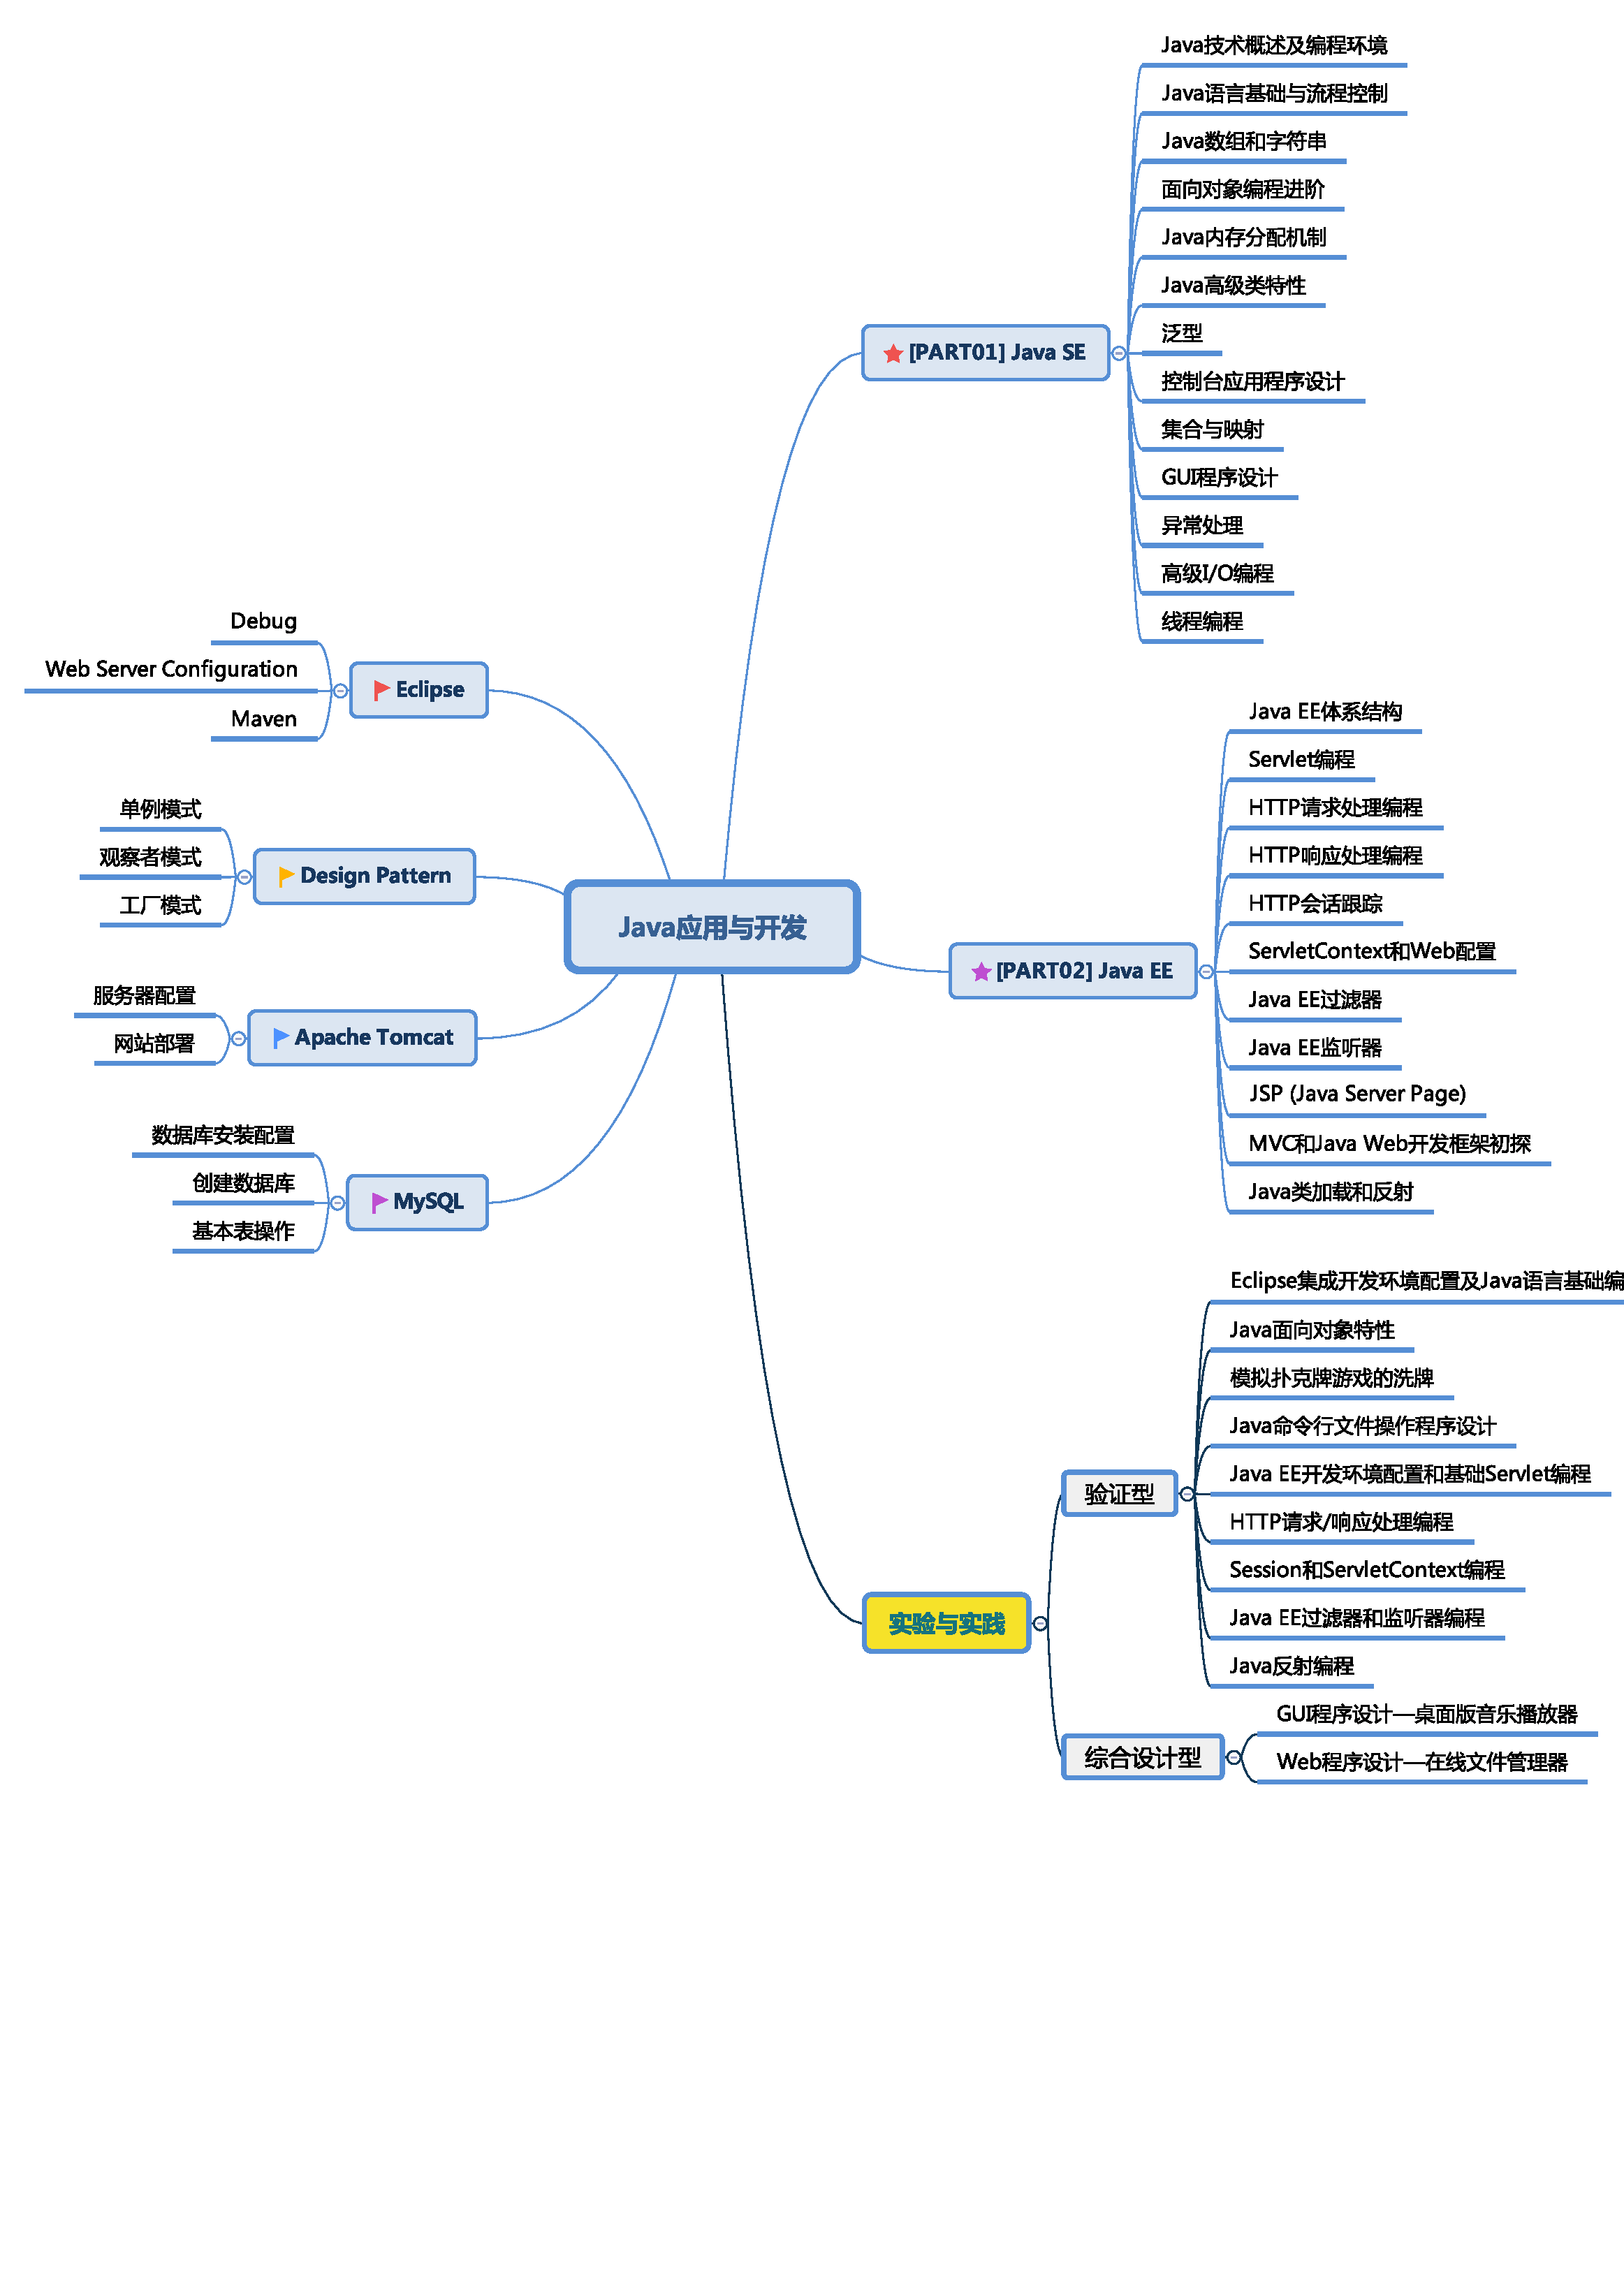
\includegraphics[width=\textwidth]{images/fig-java-course-arch.pdf}
\caption{Java应用与开发课程教学体系}
\label{fig:java-course-arch}
\end{figure}


% Week 01 %%

\chapter{Java 技术概述及开发环境}
\label{chp:Introduction-to-Java}

\section*{基本信息}
\sline
\begin{description}
\item[课程名称:] Java应用与开发
\item[授课教师:] 王晓东
\item[授课时间:] 第一周
\item[参考教材:] 本课程参考教材及资料如下:
  \begin{itemize}
  \item 陈国君主编,Java程序设计基础(第5版),清华大学出版社,2015.5
  \item Bruce Eckel, Thinking in Java (3rd)
  \end{itemize}
\end{description}

\section*{教学目标}

\sline
\begin{enumerate}
\item 讲解Java的发展历程,从Java的视角回顾OOP;
\item 理解Java平台的相关概念和机制;
\item 掌握基本的Java开发环境配置方法。
\end{enumerate}  

\section*{授课方式}

\sline
\begin{description}
\item[理论课:] 多媒体教学、程序演示
\item[实验课:] 上机编程
\end{description}

\newpage
\section*{教学内容}
\sline

\section{Java技术概述}

\subsection{Java发展简史}

Java的发展过程中伴随着多个伟大公司的起起落落。

\begin{description}
\item[\fbox{1982}] Sun公司成立(安迪$\cdot$贝托谢姆和麦克尼利)。
\item[\fbox{1986}] Sun公司上市。
\item[\fbox{1985}] Sun公司推出著名的Java语言。
\item[\fbox{2001}] 9.11事件前,Sun市值超过1000亿美元;此后,由于互联网泡沫的破碎,其市值
  在一个月内跌幅超过90\%。
\item[\fbox{2004}] Sun公司和微软在旷日持久的Java官司中和解,后者支付前者高达10亿美元的
  补偿费。
\item[\fbox{2006}] 共同创始人麦克尼利辞去CEO一职,舒瓦茨担任CEO后尝试将Sun从设备公司向软
  件服务型公司转型,但不成功。
\item[\fbox{2010}] Sun公司被甲骨文公司收购。
\end{description}

Java语言的版本迭代历程如图\ref{fig:java-versions}所示。

\begin{figure}[htb]
\centering
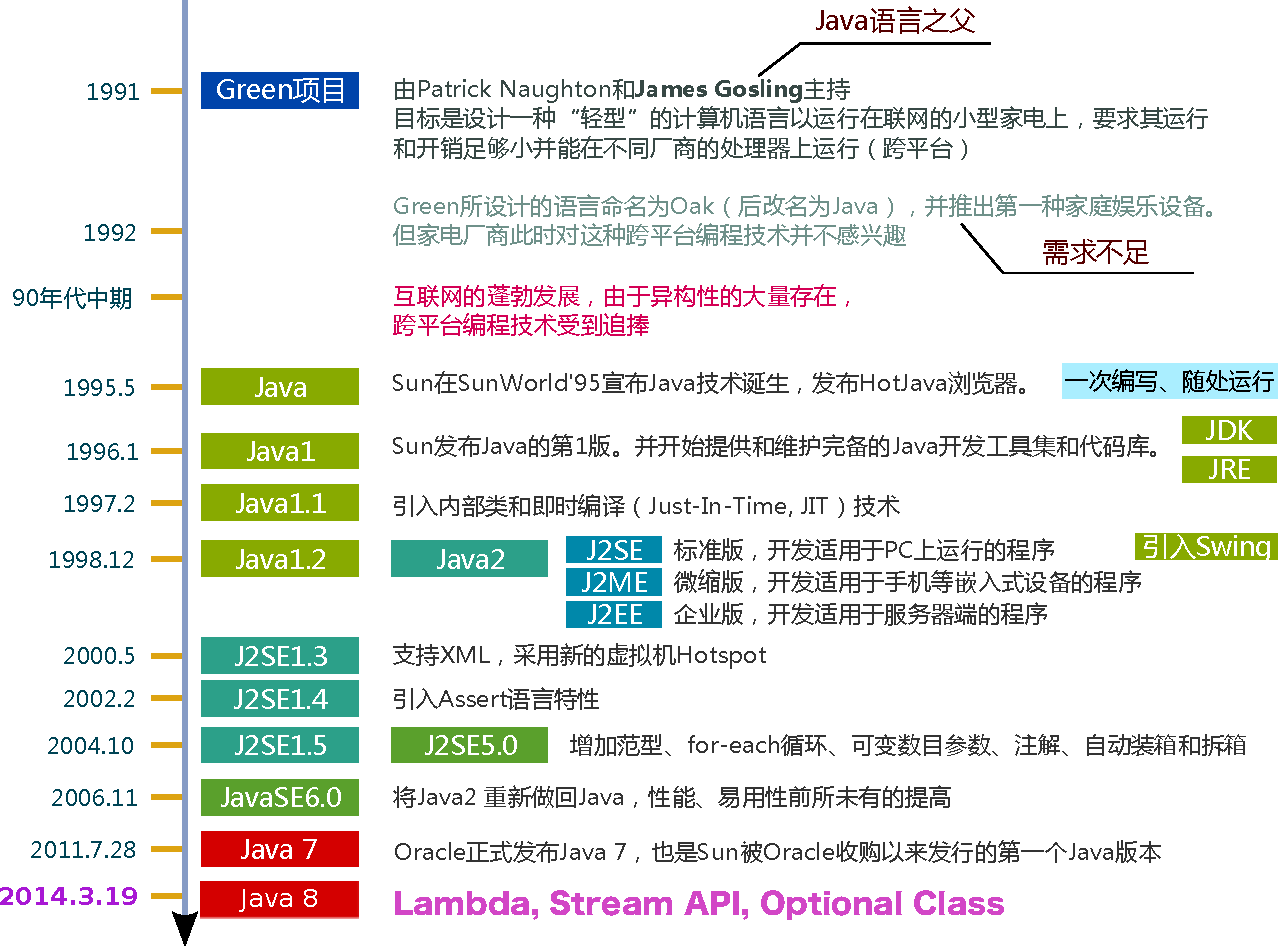
\includegraphics[width=\textwidth]{images/Introduction-to-Java/fig-java-versions.pdf}
\caption{Java版本迭代}
\label{fig:java-versions}
\end{figure}

\subsection{Java技术的特点}

Java具备以下技术特点:

\begin{description}
\item[面向对象] Java是一种以对象为中心,以消息为驱动的面向对象的编程语
  言。
\item[平台无关性] 分为源代码级(需重新编译源代码,如C/C++)和目标代码
  级(Java)平台无关。
\item[分布式] 可支持分布式技术及平台开发。
\item[可靠性] 不支持直接操作指针,避免了对内存的非法访问;自动单元回收
  功能防止内存丢失等动态内存分配导致的问题;解释器运行时实施检查,可发
  现数组和字符串访问的越界;提供了异常处理机制。
\item[多线程] C++没有内置的多线程机制,需调用操作系统的多线程功能来进行
  多线程序设计;Java提供了多线程支持。
\item[网络编程] Java具有丰富的网络编程库。
\item[编译和解释并存] 由编译器将Java源程序编译成字节码文件,再由运行系
  统解释执行字节码文件(解释器将字节码再翻译成二进制码运行)。
\end{description}

\section{Java平台核心机制}


Java技术栈如图\ref{fig:java-tech-stack}所示,程序的编译运行过程如
图\ref{fig:java-running-process}所示。需要了解以下几个核心概念:

\begin{itemize}
\item Java虚拟机
\item 垃圾回收机制
\item Java运行时环境(Java Runtime Environment, JRE)
\item JIT, Just-In-Time 传统解释器的解释执行是转换一条,运行完后就将其扔掉;
  JIT会自动检测指令的运行情况,并将使用频率高(如循环运行)的指令解释后保存下来,下次调用
  时就无需再解释(相当于局部的编译执行),显著提高了Java的运行效率。
\end{itemize}

\begin{figure}[htb]
  \begin{minipage}[t]{0.4\linewidth}
    \centering
    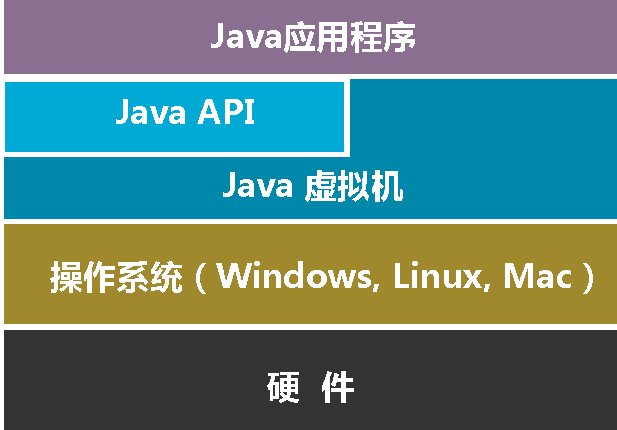
\includegraphics[width=0.9\textwidth]{images/Introduction-to-Java/fig-java-tech-stack.pdf}
    \caption{Java技术栈}
    \label{fig:java-tech-stack}
  \end{minipage}
  \begin{minipage}[t]{0.6\linewidth}
    \centering
    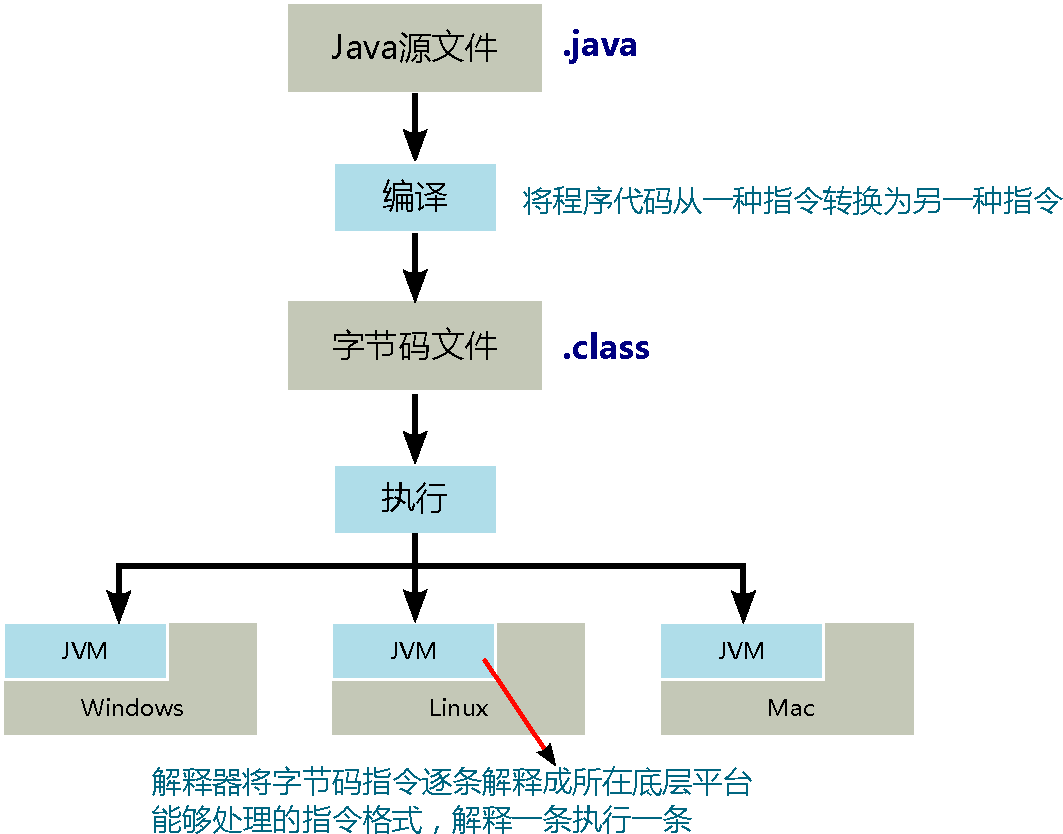
\includegraphics[width=\textwidth]{images/Introduction-to-Java/fig-java-running-process.pdf}
    \caption{Java程序编译运行过程}
    \label{fig:java-running-process}
  \end{minipage}
\end{figure}

\section{Java开发环境}
构建Java开发环境,需要首先获取和安装Java开发工具集,可以从Oracle官方网
站链
接http://www.oracle.com/technetwork/java/javase/downloads/index.html获
取。下载完成后解压放入合适的磁盘目录下。

对于Windows操作系统,可以采用以下路径:

\begin{shCode}
  D:\Program Files\Java
\end{shCode}

对于Linux操作系统,可以采用以下路径:

\begin{shCode}
  /opt/jdk1.8.0_172
\end{shCode}

接下来进行环境变量配置,以Windows操作系统为例:

\begin{description}
\item[\fbox{变量名}] Path
\item[\fbox{变量值}] D:\textbackslash Program Files\textbackslash Java\textbackslash
  jdk1.8.0\_172\textbackslash bin
\end{description}

配置完成后,可以看到JDK目录中包含以下子目录和文件:

\begin{shCode}
  bin  COPYRIGHT  db  include  javafx-src.zip
  jre  lib  LICENSE  man  README.html  release  src.zip
  THIRDPARTYLICENSEREADME-JAVAFX.txt  THIRDPARTYLICENSEREADME.txt  
\end{shCode}

对子目录的功能简要描述如下:

\begin{description}
\item[bin] Java开发工具,包括编译器、虚拟机、调试器、反编译器等;
\item[jre] Java运行时,包括Java虚拟机、类库和其他资源文件;
\item[lib] 类库和所需支持性文件;
\item[include] 用于调试本地方法(底层平台)的C++头文件;
\item[src.zip] 类库的源代码;
\item[db] Java DB数据库,JDK6.0新增项目,一种纯Java的关系型数据库。
\end{description}

\section{Java开发工具}

业界普遍采用Eclipse或IntelliJ IDEA等集成开发环境进行Java大型工程开发,
当然也可以采用文本编程工具Vim或Emacs等进行Java小型程序的开发。

本课程采用Eclipse作为首选集成开发环境。

\section{Java基本开发流程}

本部分使用文本编程工具编写一个简单的Java Hello World程序,演示Java的基
本开发和代码编译运行流程。首先,我们需要使用文本编程工具编写一个Java源
文件HelloWorld.java,文件命名必须与类名相同。

\begin{javaCode}
public class HelloWorld {
    public static void main(String[] args) {
	System.out.println("Hi, Java!");
    }
}   
\end{javaCode}

然后,使用javac工具将源文件编译为字节码文件,编译完成后,我们可以看到生成了HelloWord.class这一字节码文件。

\begin{shCode}
  > javac HelloWorld.java && ls 
  HelloWorld.class  HelloWorld.java
\end{shCode}

接下来,我们使用java工具运行该程序,在终端正确打印了“Hi, Java”字符串。

\begin{shCode}
  > java HelloWorld 
  Hi, Java!
\end{shCode}


\descript{说明}

编写Java应用程序需掌握的几条规则如下:

\begin{enumerate}
\item Java语言拼写是大小写敏感的(Case-Sensitive);
\item 一个源文件中可以定义多个Java类,但其中最多只能有一个类被定义为Public类;
\item 如果源文件中包含了public类,则源文件必须和该public类同名;
\item 一个源文件包含多个Java类时,编译后会生成多个字节码文件,即每个类都会生成一个单独的
  “.class”文件,且文件名与类名相同。
\end{enumerate}


\chapter{Java 语言基础与流程控制}
\label{chp:Java-language-basic-and-flow-control}

\section*{基本信息}
\sline
\begin{description}
\item[课程名称:] Java应用与开发
\item[授课教师:] 王晓东
\item[授课时间:] 第一周
\item[参考教材:] 本课程参考教材及资料如下:
  \begin{itemize}
  \item 陈国君主编,Java程序设计基础(第5版),清华大学出版社,2015.5
  \item Bruce Eckel, Thinking in Java (3rd)
  \end{itemize}
\end{description}

\section*{教学目标}

\sline

\begin{enumerate}
\item Java语言基础包括:数据类型、常量和变量、关键字与标识符、运算符与表达式、从键盘输入数据。
\item Java流程控制包括:语句和复合语句、分支结构(选择结构)、循环结构、跳转语句。
\end{enumerate}

\section*{授课方式}

\sline
\begin{description}
\item[理论课:] 多媒体教学、程序演示
\item[实验课:] 上机编程
\end{description}

\newpage
\section*{教学内容}
\sline

\section{Java语言基础}

\subsection{数据类型}

Java数据类型分为两大类:基本数据类型和引用数据类型。基本数据类型是由程
序设计语言系统所定义、不可再划分的数据类型。所占内存大小固定,与软硬件
环境无关,在内存中存放的是数据值本身。Java的基本数据类型包括:整型
(byte、short、int、long)、浮点型(float、double)、逻辑型(boolean)和字
符型(char)。引用数据类型(复合数据类型)在内存中存放的是指向该数据的
地址,不是数据值本身。引用数据类型包括类、数组、接口等。

数据类型的基本要素包括:

\begin{itemize}
\item 数据的性质(数据结构)
\item 数据的取值范围(字节大小)
\item 数据的存储方式
\item 参与的运算
\end{itemize}



\subsubsection{整型}

Java整型类型的数据位数及取值范围如表\ref{tab:integer-type}所示。

\begin{table}[!htbp]
  \centering
  \caption{整型数据类型}
  \label{tab:integer-type}
  \begin{tabular}{|c|c|l|}
    \hline
    {\bf 类型} & {\bf 数据位数} & {\bf 取值范围}   \\
    \hline
    byte(字节型) & 8 & $-128 \sim 127$,即$-2^{7} \sim 2^{7}-1$\\
    \hline
    short(短整型) & 16 & $-32768 \sim 32767$,即$-2^{15} \sim 2^{15}-1$\\
    \hline
    int(整型)(默认) & 32 & $-2147483648 \sim 2147483647$,即$-2^{31} \sim 2^{31}-1$\\
    \hline
    long(长整型)(l或L) & 64 & $-2^{63} \sim 2^{63}-1$\\
    \hline
  \end{tabular}
\end{table}

\subsubsection{浮点型}

Java浮点型类型的数据位数及取值范围如表\ref{tab:float-type}所示。

\begin{table}[!htbp]
  \centering
  \caption{整型数据类型}
  \label{tab:float-type}
  \begin{tabular}{|c|c|l|}
    \hline
    {\bf 类型} & {\bf 数据位数} & {\bf 取值范围}   \\
    \hline
    float(单精度)(f或F) & 32 & $1.4E-45 \sim 3.4E+38$\\
    \hline
      double(双精度)(默认) & 64 & $4.9E-324 \sim 1.8E+308$\\
    \hline
  \end{tabular}
\end{table}

\subsubsection{逻辑型}

逻辑型又称为布尔型(boolean),布尔型数据类型的特性如下:

\begin{itemize}
\item 布尔型数据只有true(真)和false(假)两个取值。
\item 布尔型数据存储占1个字节,默认取值为false。
\item 布尔型数据true和false不能转换成数字表示形式。
\end{itemize}

\subsubsection{字符型}

\begin{itemize}
\item 字符型数据类型用来存储单个字符,采用的是Unicode字符集编码方
  案\footnote{建议搜索理解什么是字符集和字符编码规则。}。
\item 字符声明用单引号表示单个字符。
\item 字符型数据可以转化为整型。
\end{itemize}

\samplecode{字符数据类型示例}
  
\begin{javaCode}
  public class CharDemo {
    public static void main(String[] args) {
      char a = 'J';
      char b='Java';  //会报错
    }
  }
\end{javaCode}
 
\subsection{数据类型转换}

\subsubsection{数值型不同类型数据的转换}

数值型不同类型数据之间的转换,{\hei 自动类型转换}需要符合以下条件:

\begin{enumerate}
\item 转换前的数据类型与转换后的类型兼容。
\item 转换后的数据类型的表示范围比转换前的类型大。
\item 条件2说明不同类型的数据进行运算时,需先转换为同一类型,然后进行运算。转换从“短”到“长”的优先关系为:\\
  byte → short → char → int → long → float → double
\end{enumerate}

如果要将较长的数据转换成较短的数据时(不安全)就要进行{\hei 强制类型转换},格式如下:

\begin{javaCode}
  (预转换的数据类型) 变量名;
\end{javaCode}

\subsubsection{字符串型数据与数值型数据相互转换}

\samplecode{字符串数据转换为数值型数据示例}

\begin{javaCode}
  String myNumber = "1234.56";
  float myFloat = Float.parseFloat(MyNumber);
\end{javaCode}

字符串可用加号“+”来实现连接操作。若其中某个操作数不是字符串,该操作在
连接之前会自动将其转换成字符串。所以可用加号来实现自动的转换。

\samplecode{数值型数据转换成字符串数据示例}

\begin{javaCode}
  int myInt = 1234;               //定义整形变量MyInt
  String myString = "" + MyInt;    //将整型数据转换成了字符串 
\end{javaCode}

\subsection{常量和变量}



\subsubsection{常量}

\begin{description}
\item[整型常量] 八进制、十六进制、十进制长整型后需要加l或L。
\item[浮点型常量] 单精度后加f或F,双精度后加d或D可省略。
\item[逻辑型常量] true或者false。
\item[字符型常量] 单引号。
\item[字符串常量] 双引号。
\end{description}

\samplecode{常量的声明}

\begin{javaCode}
  final int MAX = 10;
  final float PI =3.14f;
\end{javaCode}

\subsubsection{变量}

变量的属性包括变量名、类型、值和地址。Java语言程序中可以随时定义变量,不必集中在执行语句之前。

\samplecode{变量声明、初始化和赋值}

\begin{javaCode}
  int i, j = 0;
  i = 8;
  float k;
  k = 3.6f;
\end{javaCode}


\subsection{关键字与标识符}

Java的关键字(Java保留字)如表\ref{tab:java-key-word}所示。

\begin{table}[!htbp]
  \centering
  \caption{Java语言的关键字(保留字)}
  \label{tab:java-key-word}
  \begin{tabular}{|c|c|c|c|c|c|}
    \hline
    abstract & assert & boolean & break & byte & case \\
    \hline
    catch & char & class & continue & default & do \\
    \hline
    double & else & enum & extends & false & final \\
    \hline    
    finally & float & for & if & implements & import \\
    \hline
    instanceof & int & interface & long & native & new \\
    \hline
    null & package & private & protected & public & return \\
    \hline
    short & static & super & switch & synchronized & this \\
    \hline
    volatile & throws & transient & true & try & void \\
    \hline
  \end{tabular}
\end{table}

标识符是用来表示变量名、类名、方法名、数组名和文件名的有效字符序列。Java语言对标识符的规定如下:
  
\begin{itemize}
\item 可以由字母、数字、下划线(\_)、美元符号(\$)组合而成。
\item 必须以字母、下划线或美元符号开头,不能以数字开头。
\item 关键字不能当标识符使用。
\item 区分大小写。
\end{itemize}

建议遵循驼峰命名,类名首字母大写,变量、方法及对象首字母小写的编码习惯。

\subsection{运算符与表达式}

按照运算符功能来分,Java基本的运算符包括以下几类:

\begin{figure}[htb]
\centering
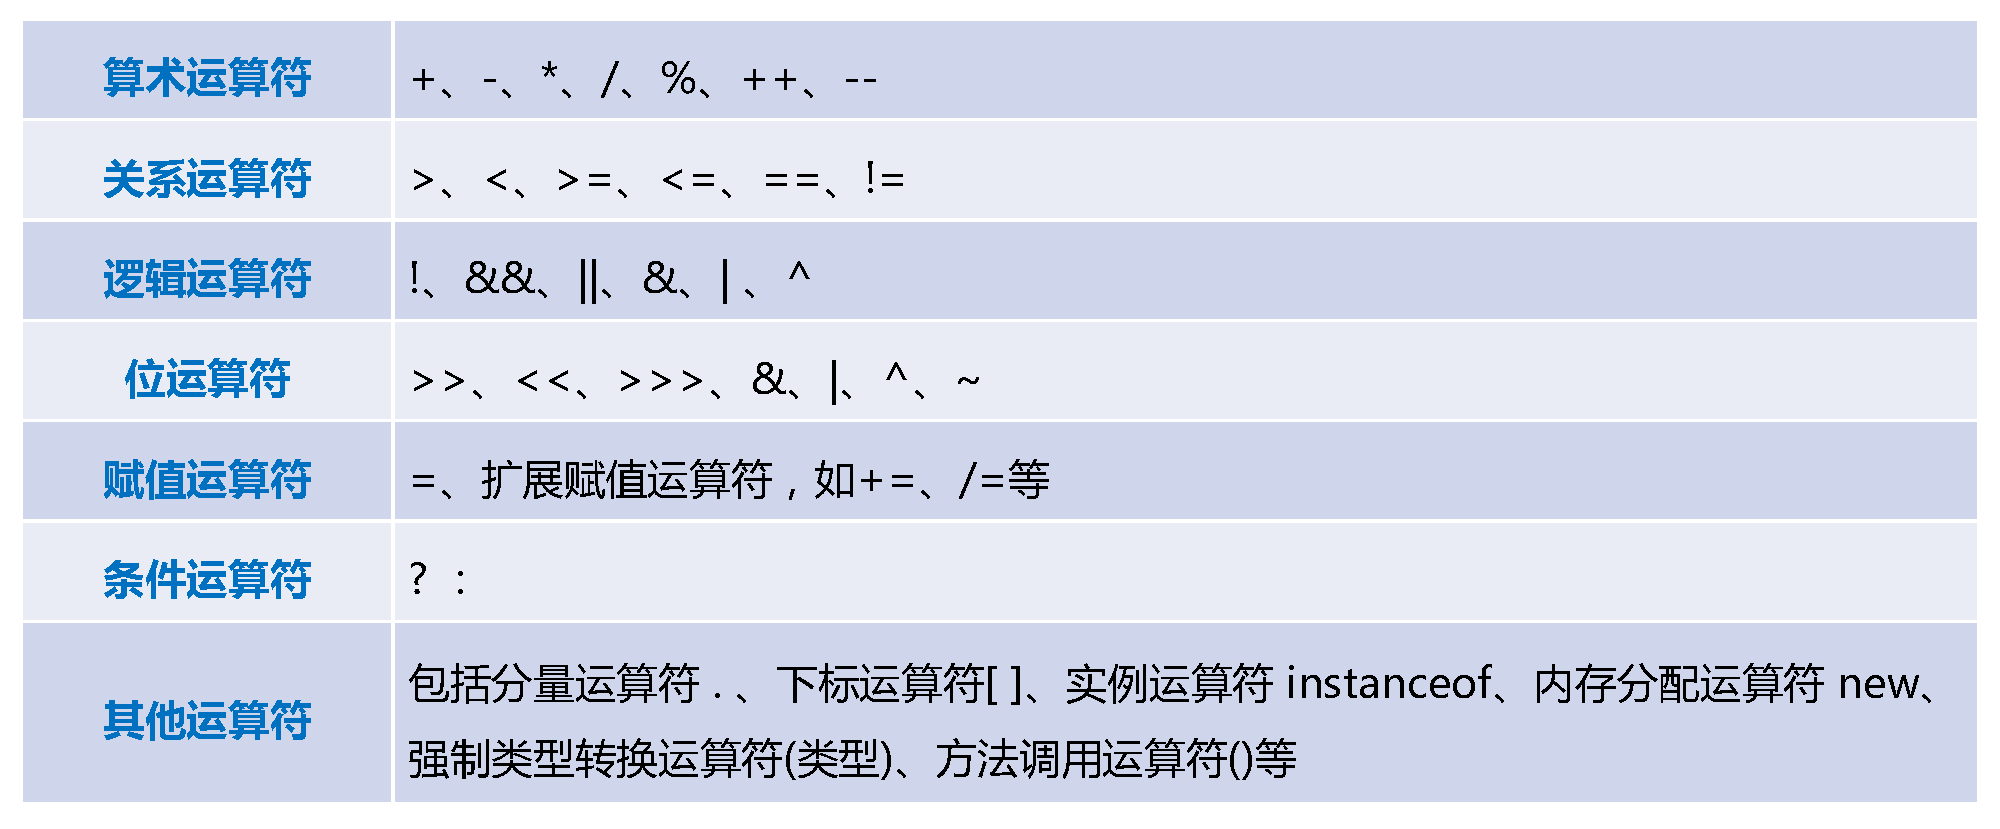
\includegraphics[width=0.9\textwidth]{images/Java-language-basic-and-flow-control/fig-java-operators.pdf}
\caption{Java运算符}
\label{fig:java-operators}
\end{figure}
  
\subsection{从键盘获得输入}

由键盘输入的数据,不管是文字还是数字,Java皆视为{\hei\Red 字符串},若是要由键盘输入获得数字则必须再经过类型转换。

\samplecode{获得键盘输入字符串并转换为数字}

\begin{javaCode}
  import java.io.*;
  public class MyClass {
    public static void main(String[] args) throws IOException {
      int num1, num2;
      String str1, str2;
      InputStreamReader in;
      in = new InputStreamReader(System.in);
      BufferedReader buf;
      buf = new BufferedReader(in);
      System.out.print("请输入第一个数:");
      str1 = buf.readLine();         //将输入的内容赋值给字符串变量 str1
      num1 = Integer.parseInt(str1);   //将 str1 转成 int 类型后赋给 num1
      System.out.print("请输入第二个数:");
      str2 = buf.readLine();         //将输入的内容赋值给字符串变量 str2
      num2 = Integer.parseInt(str2);   //将 str2 转成 int 类型后赋给 num2
      System.out.println(num1 + " * " + num2 + " = " + (num1 * num2));
    }
  }
\end{javaCode}

为了简化输入操作,从JavaSE 5版本开始在java.util类库中新增了一个类专门用
于输入操作的类{\bf\Red Scanner},可以使用该类输入一个对象。

\samplecode{使用Scanner获得键盘输入并转换为特定数据类型}

\begin{javaCode}
  import java.util.*;
  public class MyClass {
    public static void main(String[] args)
    {
      Scanner reader = new Scanner(System.in); 
      double num;
      num = reader.nextDouble(); //按照 double 类型读取键盘输入
      ...
    }
  }
\end{javaCode}

Scanner对象其他可用的数据读取方法包
括:nextByte()、nextDouble()、nextFloat()、nextInt()、nextLong()、
nextShort()、next()、nextLine()。

\section{Java流程控制}

\subsection{语句与复合语句}

\begin{itemize}
 \item Java语言中语句可以是以分号“;”结尾的简单语句,也可以是用一对花括号“\{\}”括起来的复合语句。
 \item Java中的注释形式:
   \begin{itemize}\small\Blue
   \item 单行注释://
   \item 多行注释:/*    */
   \item 文件注释:/**   */
   \end{itemize}
\end{itemize}

\subsection{分支结构}

\subsubsection{if分支结构 1}

\begin{figure}[htb]
\centering
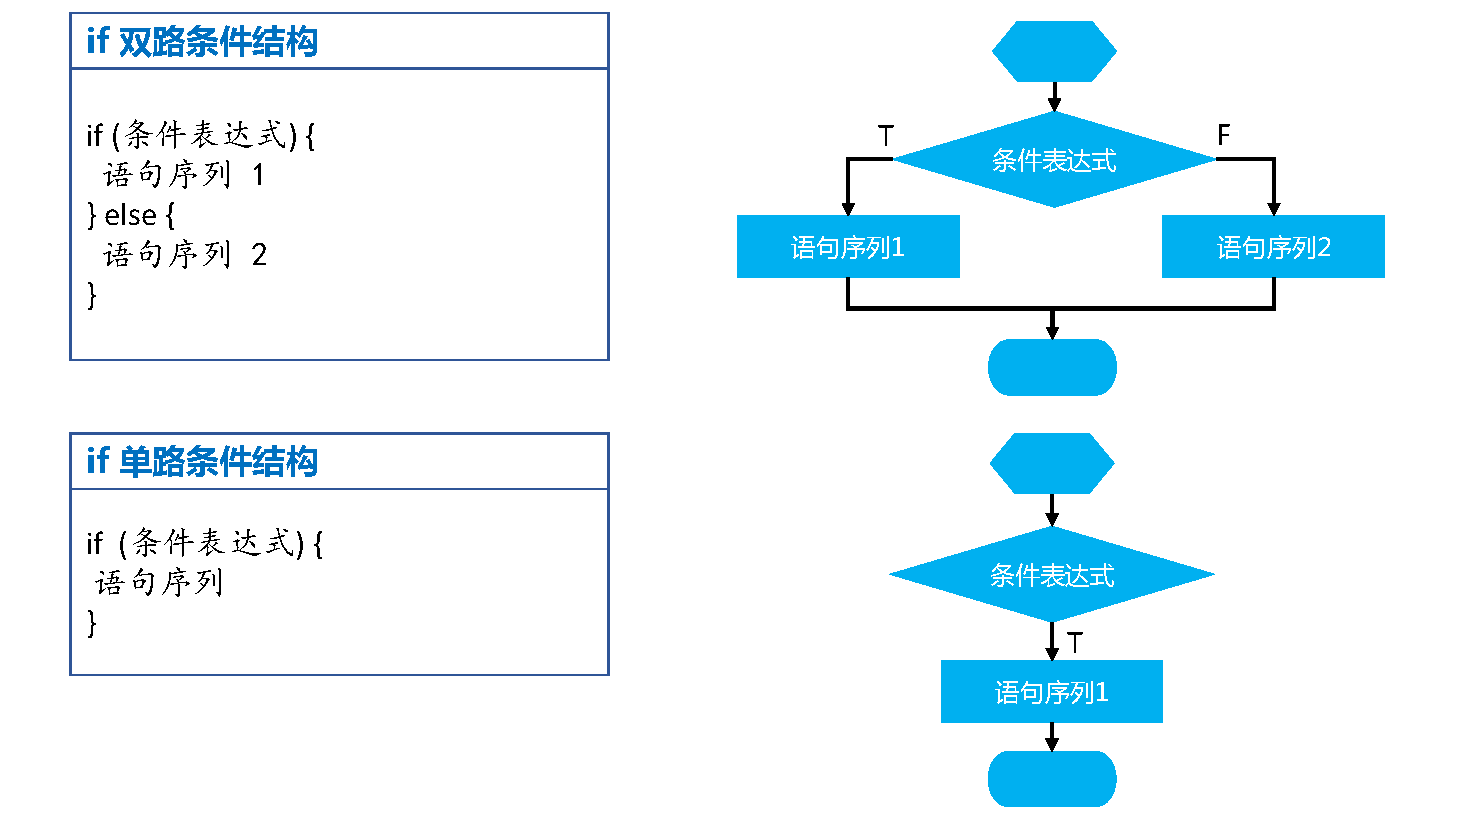
\includegraphics[width=0.9\textwidth]{images/Java-language-basic-and-flow-control/fig-if-branch-1.pdf}
\caption{if分支结构 1}
\label{fig:if-branch-1}
\end{figure}

\subsubsection{if分支结构 2}

\begin{figure}[htb]
\centering
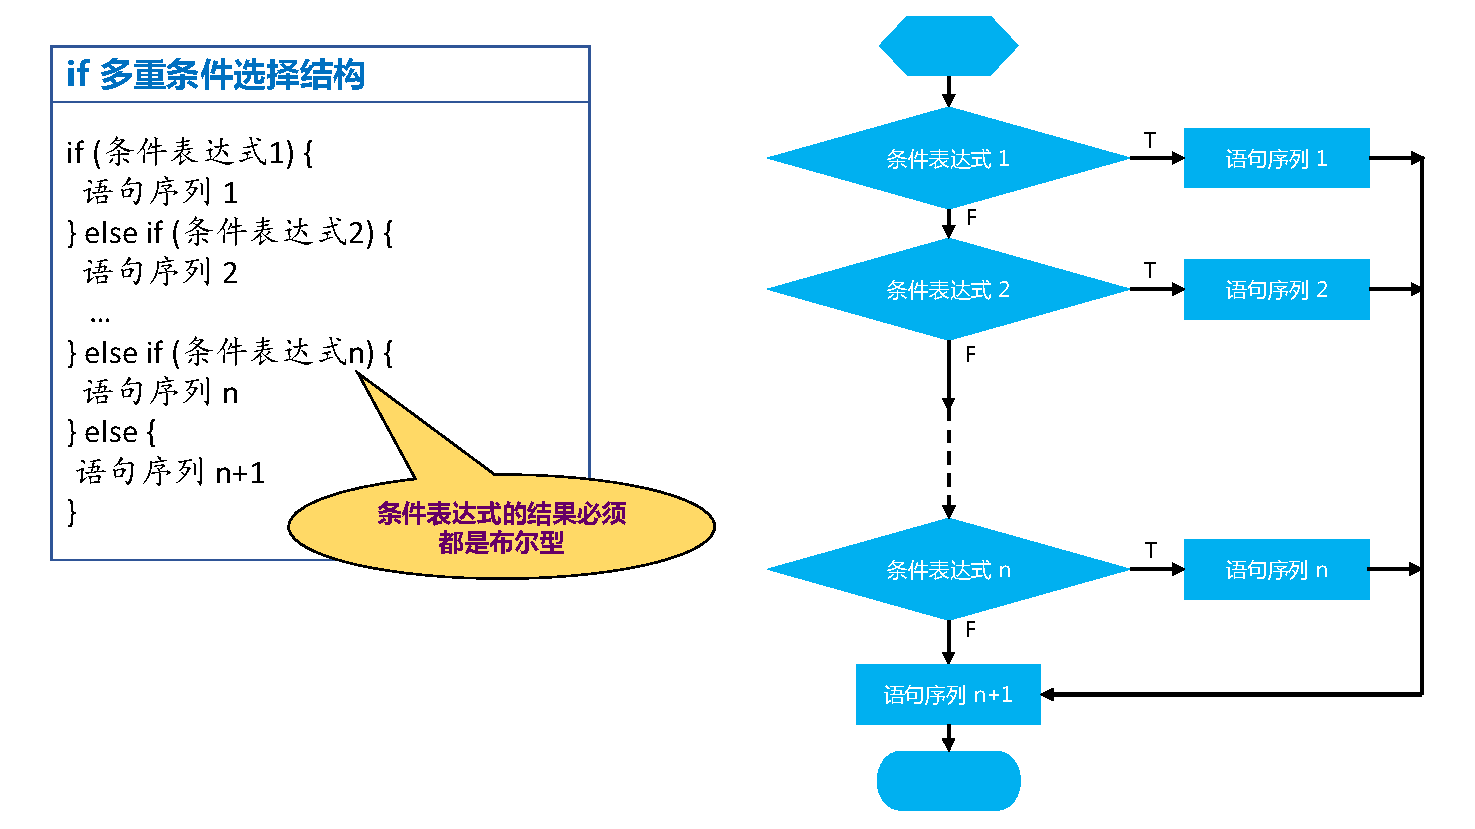
\includegraphics[width=0.9\textwidth]{images/Java-language-basic-and-flow-control/fig-if-branch-2.pdf}
\caption{if分支结构 2}
\label{fig:if-branch-2}
\end{figure}

\subsubsection{switch分支结构}

\begin{figure}[htb]
\centering
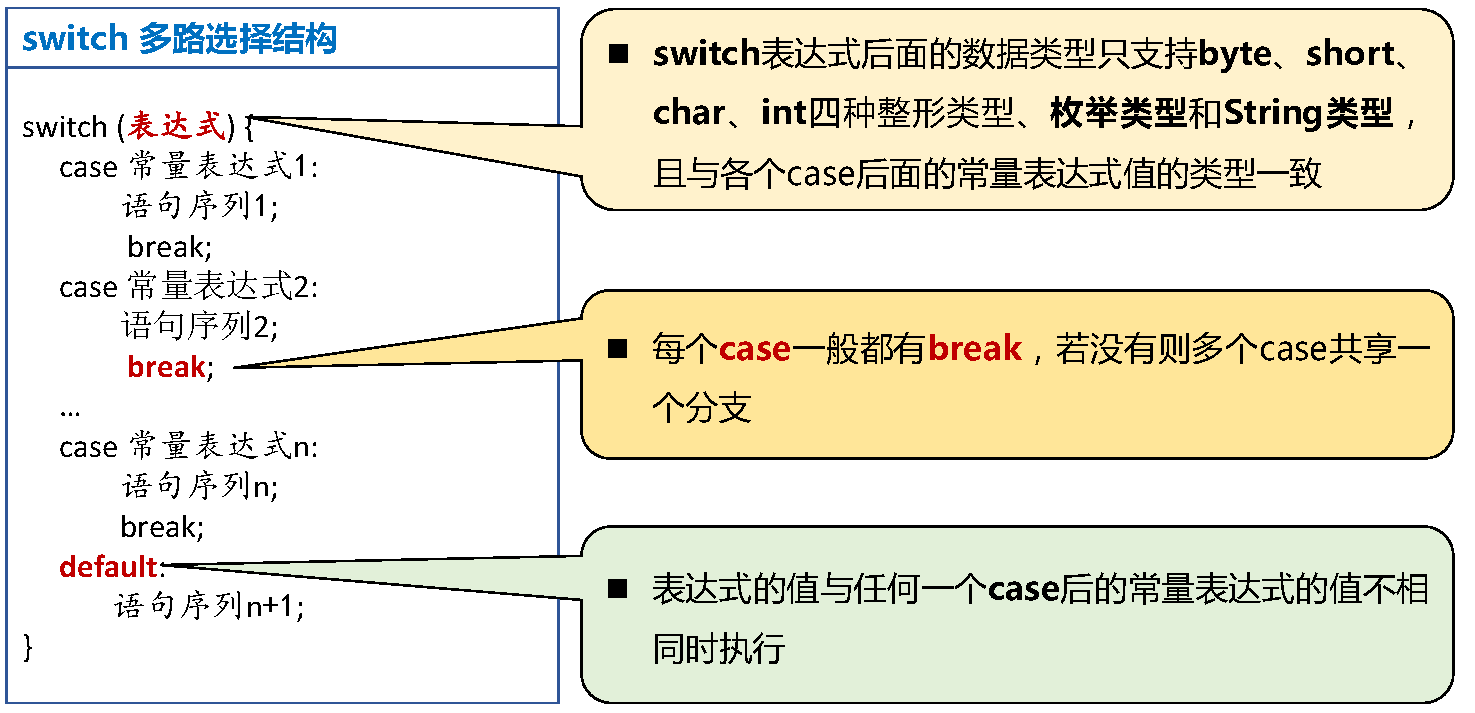
\includegraphics[width=0.9\textwidth]{images/Java-language-basic-and-flow-control/fig-switch-branch.pdf}
\caption{switch分支结构}
\label{fig:switch-branch}
\end{figure}

\descript{说明}

在Java 1.7版本之后,switch里表达式的类型可以为String。

\subsection{循环结构}

\subsubsection{while循环}

\begin{javaCode}
  while(conditional expression) {
    statements goes here ...
  }
\end{javaCode}

\subsubsection{do-while循环}

\begin{javaCode}
  do {
    statements goes here ...
  }
  while(conditional expression);
\end{javaCode}

\subsubsection{for循环 1}

\begin{javaCode}
  int[] integers = {1, 2, 3, 4};
  
  for (int j = 0; j < integers.length; j++) {
    int i = integers[j];
    System.out.println(i);
  } 
\end{javaCode}

\subsubsection{for循环 2}

\begin{javaCode}
  int[] integers = {1, 2, 3, 4};

  for (int i : integers) {
    System.out.println(i);
  }
\end{javaCode}


\subsubsection{循环中的跳转}

\begin{description}
\item[break语句] 使程序的流程从一个语句块(switch或循环结构)内跳出。
\item[continue语句] 终止当前这一轮(次)的循环,进入下一轮(次)循环。
\item[return语句] 用来使程序从方法(函数)中返回,可返回一个值。
\end{description}


\section{课后习题}

\subsection{简答题}
\begin{enumerate}
\item Java语言定义类哪些基本数据类型?其存储结构分别是什么样的?
\item 自动类型转换的前提是什么?转换时的优先级顺序如何?
\item 数字字符串转换为数值类型数据时,可以使用的方法有哪些?
\end{enumerate}

\subsection{小编程}
\begin{enumerate}
\item 编写程序,从键盘输入一个浮点数,然后将该浮点数的整数部分输出。
\item 编写程序,从键盘输入2个整数,然后计算它们相除后得到的结果并输出,注意排除0除问题。
\end{enumerate}
\chapter*{实验设计}
\sline

\begin{description}
\item[实验名称:] Eclipse集成开发环境配置及Java语言基础编程练习
\item[上机时间:] 第一周
\item[实验手册:] 无(参照实验内容完成)
\item[实验内容:] 本次实验需要完成以下内容:
  \begin{enumerate}
  \item 使用文本编辑器完成Java Hello World程序编写,使用javac和java编译运行该程序;
  \item 熟悉Eclipse集成开发环境,学习创建Java工程,使用Maven创建Java工程;
  \item 根据授课幻灯片和讲义,尝试实现其中所有的示例代码。
  \end{enumerate}
  
\item[实验要求:] 本次实验不需要提交实验报告。
\end{description}

% Week 02 %%
\chapter{Java 数组和字符串}
\label{chp:Java-array-and-string}

\section*{基本信息}
\sline
\begin{description}
\item[课程名称:] Java应用与开发
\item[授课教师:] 王晓东
\item[授课时间:] 第二周
\item[参考教材:] 本课程参考教材及资料如下:
  \begin{itemize}
  \item 陈国君主编,Java程序设计基础(第5版),清华大学出版社,2015.5
  \item Bruce Eckel, Thinking in Java (3rd)
  \end{itemize}
\end{description}

\section*{教学目标}

\sline

\begin{enumerate}
\item 掌握Java数组的概念
\item 学会一维数组和二维数组的使用;认识Arrays类,掌握操作数组相关方法
\item 掌握Java字符串的概念,字符串与数组的关系;学会String类常用字符串操作方法
\end{enumerate}

\section*{授课方式}

\sline
\begin{description}
\item[理论课:] 多媒体教学、程序演示
\item[实验课:] 上机编程
\end{description}

\newpage
\section*{教学内容}
\sline

\section{数组的概念}

数组是相同数据类型的元素按一定顺序排列的集合。在Java语言中,数组元素既可以为基本数据类型,也可以为对象。

\kgtip{Java的内存分配(基础)}

\begin{description}
\item [栈内存] 存放定义的基本类型的变量和对象的引用变量,超出作用域将自动释放。
\item [堆内存] 存放由new运算符创建的对象和数组,由Java虚拟机的自动垃圾回收器来管理。
\end{description}

Java数组的主要特点包括以下方面:

\begin{itemize}
\item 数组是相同数据类型的元素的集合;
\item 数组中的各元素有先后顺序,它们在内存中按照这个先后顺序连续存放;
\item 数组的元素用整个数组的名字和它自己在数组中的顺序位置来表示。
\end{itemize}

{\Blue\kai 例如,a[0]表示名字为a的数组中的第一个元素,a[1]表示数组a的第二个元素,依次类推。}

\section{一维数组}

\subsection{创建数组}

创建Java数组一般需经过三个步骤:

\begin{enumerate}
\item 声明数组;
\item 创建内存空间;
\item 创建数组元素并赋值。
\end{enumerate}

\samplecode{一维数组创建声明和内存分配}

\begin{javaCode}
  int[] x;  //声明名称为x的int型数组,未分配内存给数组
  x = new int[10];   //x中包含有10个元素,并分配空间
\end{javaCode}

\begin{javaCode}
  int[] x = new int[10];   //声明数组并动态分配内存
\end{javaCode}

\descript{说明}

用new分配内存的同时,数组的每个元素都会自动赋默认值,整型为0,实数为0.0,布尔型为false,引用型为null。

\subsection{一维数组的初始化}

若在声明数组时进行赋值即初始化,称为静态内存分配。

\begin{javaCode}
  数据类型[] 数组名 = {初值0,初值1,…,初值n};
\end{javaCode}

\samplecode{一维数组静态初始化}

\begin{javaCode}
  int[] a = {1,2,3,4,5};
\end{javaCode}

\descript{注意}

在Java程序中声明数组时,无论用何种方式定义数组,都不能指定其长度。

\section{二维数组}

Java中无真正的多维数组,只是数组的数组。

\subsection{二维数组的声明和内存分配}

\begin{javaCode}
  数据类型[][] 数组名;
  数组名 = new 数据类型 [行数][列数];
  数据类型[][] 数组名 = new 数据类型 [行数][列数];
\end{javaCode}

\begin{figure}[htb]
\centering
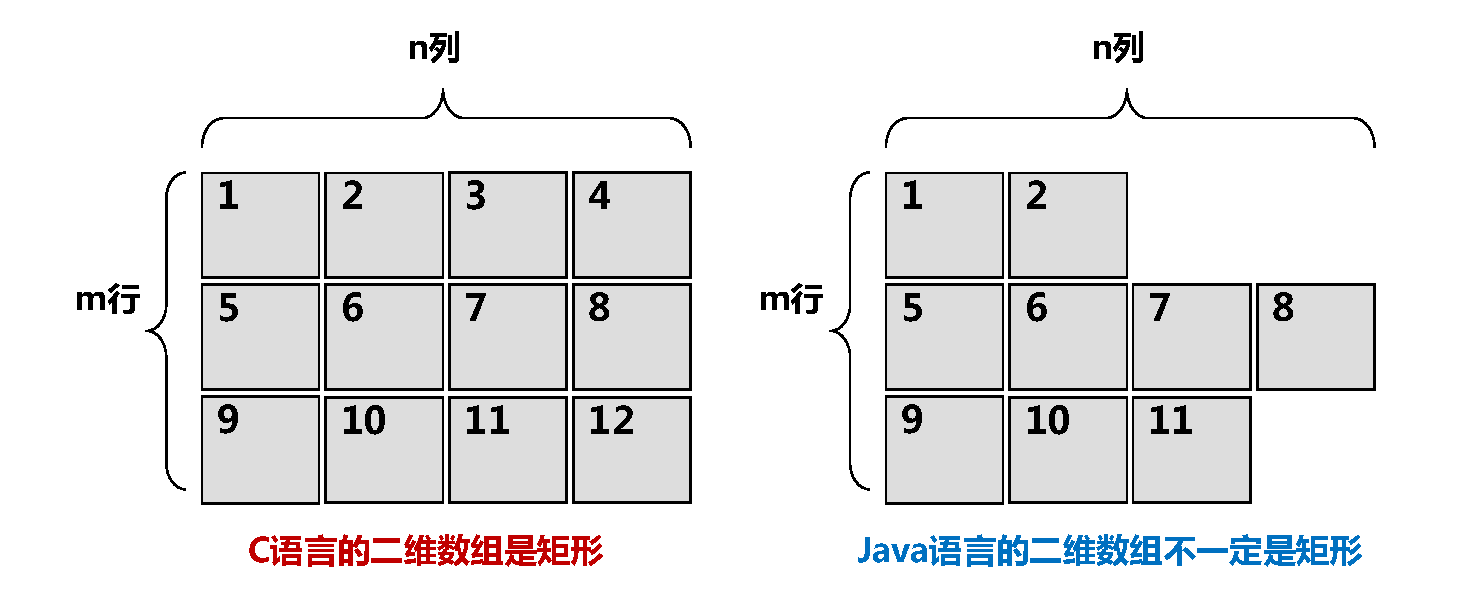
\includegraphics[width=\textwidth]{images/Java-array-and-string/fig-2-dim-array.pdf}
\caption{Java版本迭代}
\label{fig:java-versions}
\end{figure}

\subsection{二维数组定义的含义}

\begin{itemize}
\item Java中的二维数组看作是由多个一维数组构成
\item 二维数组申请内存必须指定{\Red 高层维数}\\
  \fbox{int[][] myArray1 = new int[10][];}\\
  \fbox{int[][] myArray2 = new int[10][3];}
\item \fbox{int[][] x;}\\
  {\kai\Blue 表示定义了一个数组引用变量x,第一个元素为x[0],最后一个为x[n-1],其长度不确定}
\item \fbox{x = new int[3][];}\\
  {\kai\Blue 表示数组x有三个元素,每个元素都是int[]类型的一维数组,分别为int x[0][]、int[] x[1]、int[] x[2]}\\
  \fbox{x[0] = new int[3];  x[1] = new int[2];}\\
  {\kai\Blue 给x[0]、x[1]、x[2]赋值(长度可以不一样)}
\end{itemize}

\subsection{二维数组赋初值}

\begin{javaCode}
  int[][] a = {{11,22,33,44}, {66,77,88,99}};
\end{javaCode}

\descript{注意}

声明多维数组并初始化时不能指定其长度,否则出错。



\section{Arrays类}

java.util.Arrays工具类能方便地操作数组,它提供的所有方法都是静态的。该类具有以下功能:

\begin{description}
\item[给数组赋值] 通过fill方法。
\item[对数组排序] 通过sort方法。
\item[比较数组] 通过equals方法比较数组中元素值是否相等。
\item[查找数组元素] 通过binarySearch方法能对排序好的数组进行二分查找法操作。
\item[复制数组] 把数组复制成一个长度为length的新数组。
\end{description}

\samplecode{Array操作示例}

\begin{javaCode}
  /*
  * 数组比较 equals
  */
  String[] str1 = { "1", "2", "3" };
  String[] str2 = { "1", "2", new String("3") };
  System.out.println(Arrays.equals(str1, str2)); // 结果是true

  /*
  * 数组排序 sort
  */
  int[] score = { 79, 65, 93, 64, 88 };

  // 将数组转换为字符串
  String str = Arrays.toString(score);
  System.out.println("原数组为:" + str);

  Arrays.sort(score); // 作用是把一个数组按照有小到大进行排序,会改变原score而不是创建新对象

  // 将数组转换为字符串
  System.out.println("排序后数组为:" + Arrays.toString(score));

  /*
  * 把数组中的所有元素替换成一个值 fill
  */
  int[] num = { 1, 2, 3 };
  Arrays.fill(num, 6); // 参数1:数组对象;参数2:替换的值
  System.out.println(Arrays.toString(num)); // 打印结果:[6, 6, 6]

  /*
  * 通过二分法查询元素值在数组中的下标 binarySearch
  */
  char[] a = { 'a', 'b', 'c', 'd', 'e' };
  int i = Arrays.binarySearch(a, 'd');
  System.out.println(i); // 结果是:3

  char[] b = { 'e', 'a', 'c', 'b', 'd' };
  Arrays.sort(b);
  int j = Arrays.binarySearch(b, 'e');
  System.out.println(j); // 结果是:4

  /*
  * 把数组内容复制到一个新数组中 copyOf
  */
  int[] c = { 1, 2, 3 };
  int[] d = Arrays.copyOf(c, c.length + 2); // 参数1:原数组 参数2:新数组的长度
  System.out.println("原数组为:" + Arrays.toString(c));
  System.out.println("复制后的新数组为:" + Arrays.toString(d));  
\end{javaCode}


\section{字符串}

字符串是用一对双引号括起来的字符序列。Java语言中,字符串常量或变量均用类实现。

\subsection{字符串变量的创建}

\samplecode{格式1}

\begin{javaCode}
  String s;                  //声明字符串型引用变量s,此时s的值为null
  s = new String("Hello");   //在堆内存中分配空间,并将s指向该字符串首地址
\end{javaCode}

\samplecode{格式2}

\begin{javaCode}
  String s = new String("Hello");
\end{javaCode}

\samplecode{格式3}

\begin{javaCode}
  String s = "Hello";
\end{javaCode}

\subsection{String类的常用方法}

\samplecode{求字符串长度}

\begin{javaCode}
  String str = new String("asdfzxc");
  int strlength = str.length(); //strlength = 7
\end{javaCode}

\samplecode{获取字符串某一位置字符}

\begin{javaCode}
  char ch = str.charAt(4); //ch = z
\end{javaCode}

\samplecode{提取子串}

\begin{javaCode}
  String str2 = str1.substring(2); //str2 = "dfzxc"
  String str3 = str1.substring(2,5); //str3 = "dfz"
\end{javaCode}

\samplecode{字符串连接}

\begin{javaCode}
  String str = "aa".concat("bb").concat("cc");
  String str = "aa" + "bb" + "cc"; // 相当于上一行
\end{javaCode}


\samplecode{字符串比较}

\begin{javaCode}
  String str1 = new String("abc");
  String str2 = new String("ABC");
  int a = str1.compareTo(str2);  //a>0
  int b = str1.compareTo(str2);  //b=0
  boolean c = str1.equals(str2); //c=false
  boolean d = str1.equalsIgnoreCase(str2); //d=true
\end{javaCode}

\samplecode{字符串中字符的大小写转换}

\begin{javaCode}
  String str = new String("asDF");
  String str1 = str.toLowerCase(); //str1 = "asdf"
  String str2 = str.toUpperCase(); //str2 = "ASDF"
\end{javaCode}

\samplecode{字符串中字符的替换}

\begin{javaCode}
  String str = "asdzxcasd";
  String str1 = str.replace('a','g'); //str1 = "gsdzxcgsd"
  String str2 = str.replace("asd","fgh"); //str2 = "fghzxcfgh"
  String str3 = str.replaceFirst("asd","fgh"); //str3 = "fghzxcasd"
  String str4 = str.replaceAll("asd","fgh"); //str4 = "fghzxcfgh"
\end{javaCode}

\subsection{理解Java字符串}

\samplecode{String.java部分代码}

\begin{javaCode}
  public final class String
  implements java.io.Serializable, Comparable<String>, CharSequence { //1

    /** The value is used for character storage. */
    private final char value[]; //2
    
    /** The offset is the first index of the storage that is used. */
    private final int offset;
    
    /** The count is the number of characters in the String. */
    private final int count;
    
    /** Cache the hash code for the string */
    private int hash; // Default to 0

    /** use serialVersionUID from JDK 1.0.2 for interoperability */
    private static final long serialVersionUID = -6849794470754667710L;
    ........

    public String substring(int beginIndex, int endIndex) { //3
      if (beginIndex < 0) {
        throw new StringIndexOutOfBoundsException(beginIndex);
      }
      if (endIndex > count) {
        throw new StringIndexOutOfBoundsException(endIndex);
      }
      if (beginIndex > endIndex) {
        throw new StringIndexOutOfBoundsException(endIndex - beginIndex);
      }
      return ((beginIndex == 0) && (endIndex == count)) ? this :
      new String(offset + beginIndex, endIndex - beginIndex, value);
    }
}
\end{javaCode}

\begin{enumerate}
\item String类是final类,即意味着String类不能被继承,并且它的成员方法都默认为final方法。
\item 从String类的成员属性可以看出String类其实是通过char数组来保存字符串的。
\item 无论是substring还是concat操作等都不是在原有的字符串上进行的,而是重新生成了一个新的字符串对象,最原始的字符串并没有被改变。

\end{enumerate}

\descript{说明}

String对象一旦被创建就是固定不变的,对String对象的任何操作都不影响到原对象,而是会生成新的对象。
\chapter{Java 面向对象编程进阶 A}
\label{chp:Advanced-object-oriented-programming}

\section*{基本信息}
\sline
\begin{description}
\item[课程名称:] Java应用与开发
\item[授课教师:] 王晓东
\item[授课时间:] 第二周(根据校历,本周有两次课)
\item[参考教材:] 本课程参考教材及资料如下:
  \begin{itemize}
  \item 陈国君主编,Java程序设计基础(第5版),清华大学出版社,2015.5
  \item Bruce Eckel, Thinking in Java (3rd)
  \end{itemize}
\end{description}

\section*{教学目标}

\sline

\begin{enumerate}
\item 掌握Java包、继承、访问控制、方法重写的概念、机制和使用方法
\item 理解Java关键字super和关键字this,特别了解其指代的对象,编程中的用法
\end{enumerate}

\section*{授课方式}

\sline
\begin{description}
\item[理论课:] 多媒体教学、程序演示
\item[实验课:] 上机编程
\end{description}

\newpage
\section*{教学内容}
\sline

%%%%%%%%%%%%%%%%%%%%%%%%%%%%%%%%%%%%%%%%%%%%%%%%%%%%%%%%%%%%%%
\section{包}
为便于管理大型软件系统中数目众多的类,解决类的命名冲突问题以及进行访问
控制,Java引入包(package)机制,即将若干功能相关的类逻辑上分组打包到一
起,提供类的多重类命名空间。

\begin{figure}[htb]
\centering
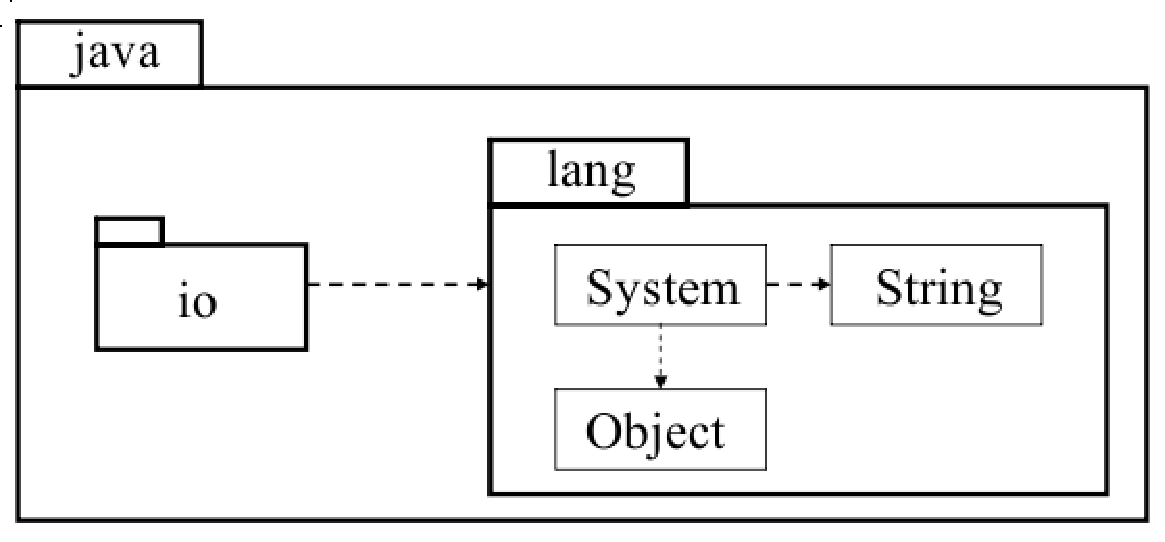
\includegraphics[width=0.6\textwidth]{images/Advanced-object-oriented-programming-1/fig-java-package.pdf}
\caption{Java包}
\label{fig:java-package}
\end{figure}

\subsection{JDK常用包}

JDK API中的常用包如表所示。

\begin{table}[!htbp]
  \centering
  \caption{JDK API常用包}
  \label{tab:java-package-list}
  \begin{tabular}{|c|c|c|}
    \hline
    {\bf 包名} & {\bf 功能说明} & {\bf 包的含义}   \\
    \hline
    java.lang & Java语言程序设计的基础类 & language的简写\\
    \hline
    java.awt & 创建图形用户界面和绘制图形图像的相关类 & 抽象窗口工具集\\
    \hline
    java.util & 集合、日期、国际化、各种实用工具 & utility的简写\\
    \hline
    java.io & 可提供数据输入/输出相关功能的类 & input/output的简写\\
    \hline
    java.net & Java网络编程的相关功能类 & 网络\\
    \hline
    java.sql & 提供数据库操作的相关功能类 & 结构化查询语言的简写\\
    \hline
  \end{tabular}
\end{table}


\subsection{包的创建}

package语句作为Java源文件的第一条语句,指明该文件中定义的类所在的包(若缺省该语句,则指定为无名包)。语法格式如下:

\begin{javaCode}
  package pkg1[.pkg2[.pkg3...]];
\end{javaCode}

\samplecode{创建包}

\begin{javaCode}
  package p1;
  public class Test {
    public void m1() {
      System.out.println("In class Test, method m1 is running!");
    }
  }
\end{javaCode}

package语句对所在源文件中定义的所有类型(包括接口、枚举、注解)均起作用。

Java编译器把包对应于文件系统的目录管理,package语句中,用“.”来指明包(目录)的层次。如果在程序Test.java中已定义了包p1,编译时采用如下方式:

\begin{shCode}
  > javac Test.java
\end{shCode}

则编译器会在当前目录下生成Test.class文件。

若在命令行下使用如下命令:

\begin{shCode}
  > java -d /home/xiaodong/work01 Test.java
\end{shCode}

“-d /home/xiaodong/work01”是传给Java编译器的参数,用于指定此次编译生成的.class文件保存到
该指定路径下,并且如果源文件中有package语句,则编译时会自动在目标路径下创建与包同名的目
录p1,再将生成的Test.class文件保存到该目录下。

\subsection{导入包中的类}

为使用定义在不同包中的Java类,需用import语句来引入所需要的类。语法格式:

\begin{javaCode}
  import pkg1[.pkg2...].(classname|*);  
\end{javaCode}

\samplecode{导入和使用有名包中的类}

\begin{javaCode}
  import p1.Test; //or import p1.*;
  public class TestPackage{
    public static void main(String args[]){
      Test t = new Test();
      t.m1();
    }
  }
\end{javaCode}

\subsection{Java包特性}

一个类如果未声明为public的,则只能在其所在包中被使用,其他包中的类即使
在源文件中使用import语句也无法引入它。可以不在源文件开头使用import语句
导入要使用的有名包中的类,而是在程序代码中每次用到该类时都给出其完整的
包层次,例如:

\begin{javaCode}
  public class TestPackage{ 
    public static void main(String args[]){ 
      p1.Test t = new p1.Test(); 
      t.m1(); 
    } 
  }
\end{javaCode}

%%%%%%%%%%%%%%%%%%%%%%%%%%%%%%%%%%%%%%%%%%%%%%%%%%%%%%%%%%%%%%
\section{继承}

\subsection{继承的概念}

继承(Inheritance)是面向对象编程的核心机制之一,其本质是在已有类型基础
之上进行扩充或改造,得到新的数据类型,以满足新的需要。

根据需要定义Java类描述“人”和“学生”信息,示例代码如下:

\samplecode{Class Person}
\begin{javaCode}
  public class Person {
    public String name;
    public int age;
    public Date birthDate;
    public String getInfo() {...}
  }
\end{javaCode}

\samplecode{Class Student}

\begin{javaCode}
  public class Student {
    public String name;
    public int age;
    public Date birthDate;
    public String school;
    public String getInfo() {...}
  }
\end{javaCode}

我们可以通过继承简化Student类的定义:

\samplecode{Class Student extends Person}

\begin{javaCode}
  public class Student extends Person {
    public String school;
  }
\end{javaCode}

Java类声明的语法格式如下:

\begin{javaCode}
  [< 修饰符 >] class < 类名 > [extends < 父类名 >] {
    [< 属性声明 >]
    [< 构造方法声明 >]
    [< 方法声明 >]
  }
\end{javaCode}

Object类是所有Java类的最高层父类,如果在类的声明中未使用extends关键字指明其父类,则默认父类为Object类。

Java只支持单继承,不允许多重继承。即:

\begin{itemize}
\item 一个子类只能有一个父类;
\item 一个父类可以派生出多个子类。
\end{itemize}

\begin{figure}[htb]
\centering
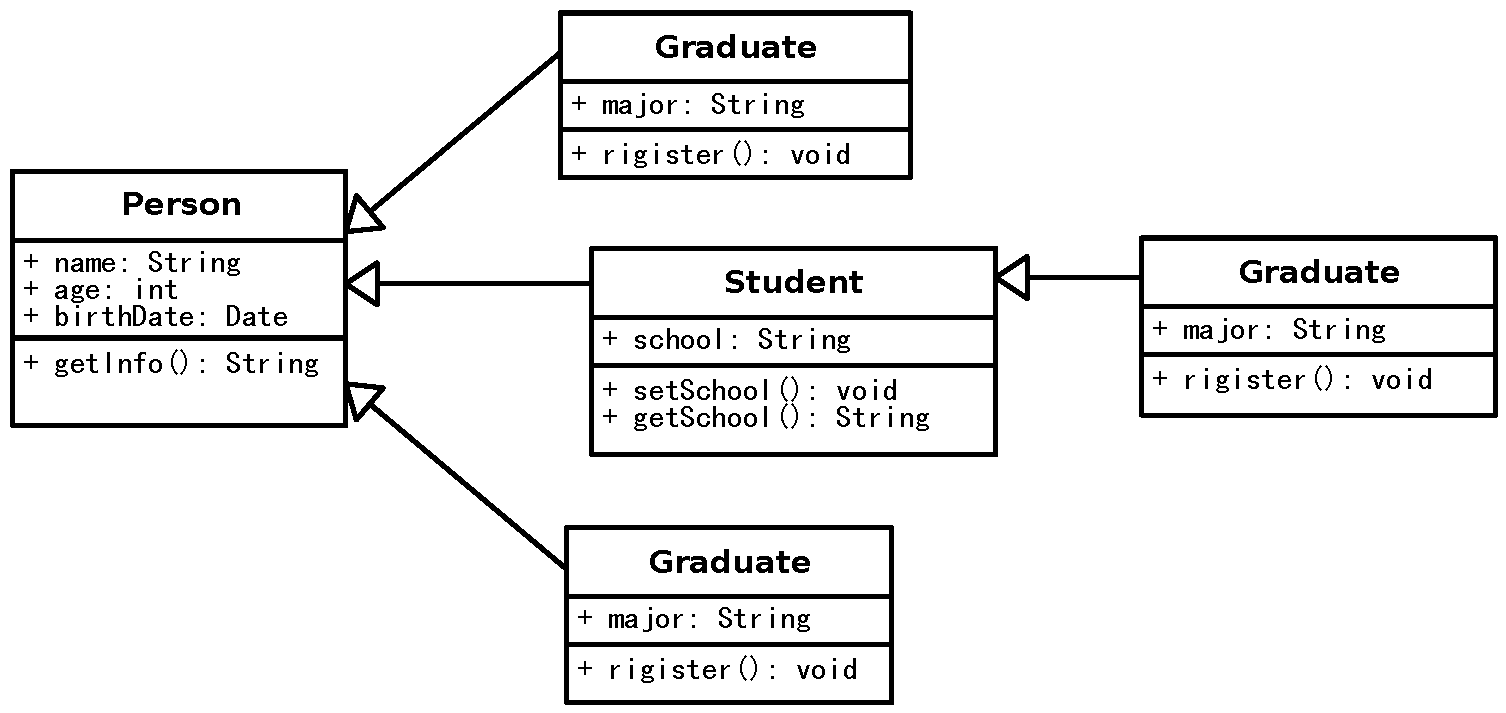
\includegraphics[width=0.9\textwidth]{images/Advanced-object-oriented-programming-1/fig-java-extends.pdf}
\caption{Java包}
\label{fig:java-package}
\end{figure}

\subsection{类之间的关系}

\begin{description}
\item[依赖关系] 一个类的方法中使用到另一个类的对象
  (uses-a)\footnote{车能够装载货物,车的装载功能(load()方法)对货物
    (goods)有依赖。}。
\item[聚合关系] 一个类的对象包含(通过属性引用)了另一个类的对象
  (has-a)\footnote{车有发动机、车轮等,Car对象是由Engine等对象构成
    的。}。
\item[泛化关系] 一般化关系(is-a),表示类之间的继承关系、类和接口之间
  的实现关系以及接口之间的继承关系。
\end{description}

\section{访问控制}

访问控制是指对Java类或类中成员的操作进行限制,即规定其在多大的范围内可以被直接访问。

\subsection{类的访问控制}

在声明Java类时可以在class关键字前使用public来修饰,也可以不使用该修饰
符。public的类可在任意场合被引入和使用,而非public的类只能在其所在包中
被使用。

\subsection{类中成员的访问控制}

\begin{table}[!htbp]
  \centering
  \caption{类成员的访问控制}
  \label{tab:java-class-member-access-control}
  \begin{tabular}{|c|c|c|c|c|}
    \hline
    {\bf 修饰符/作用范围} & {\bf 同一个类} & {\bf 同一个包} & {\bf 子类} & {\bf 任何地方} \\
    \hline
    public & yes & yes & yes & yes\\
    \hline
    protected  & yes & yes & yes & no \\
    \hline
    无修饰符 & yes & yes & no & no \\
    \hline
    private & yes & no & no & no \\
    \hline
  \end{tabular}
\end{table}

\subsection{访问控制注意的一些问题}

\begin{itemize}
\item 一般不提倡将属性声明为public的,而构造方法和需要外界直接调用的普通方法则适合声明为
  public的。
\item 在位于不同的包内,必须是子类的对象才可以直接访问其父类的protected成员,而父类自身
  的对象反而不能访问其所在类中声明的protected成员。
\item 所谓“访问控制”只是控制对Java类或类中成员的直接访问,而间接访问是不做控制的,也不该
  进行控制。
\end{itemize}

\begin{figure}[htb]
\centering
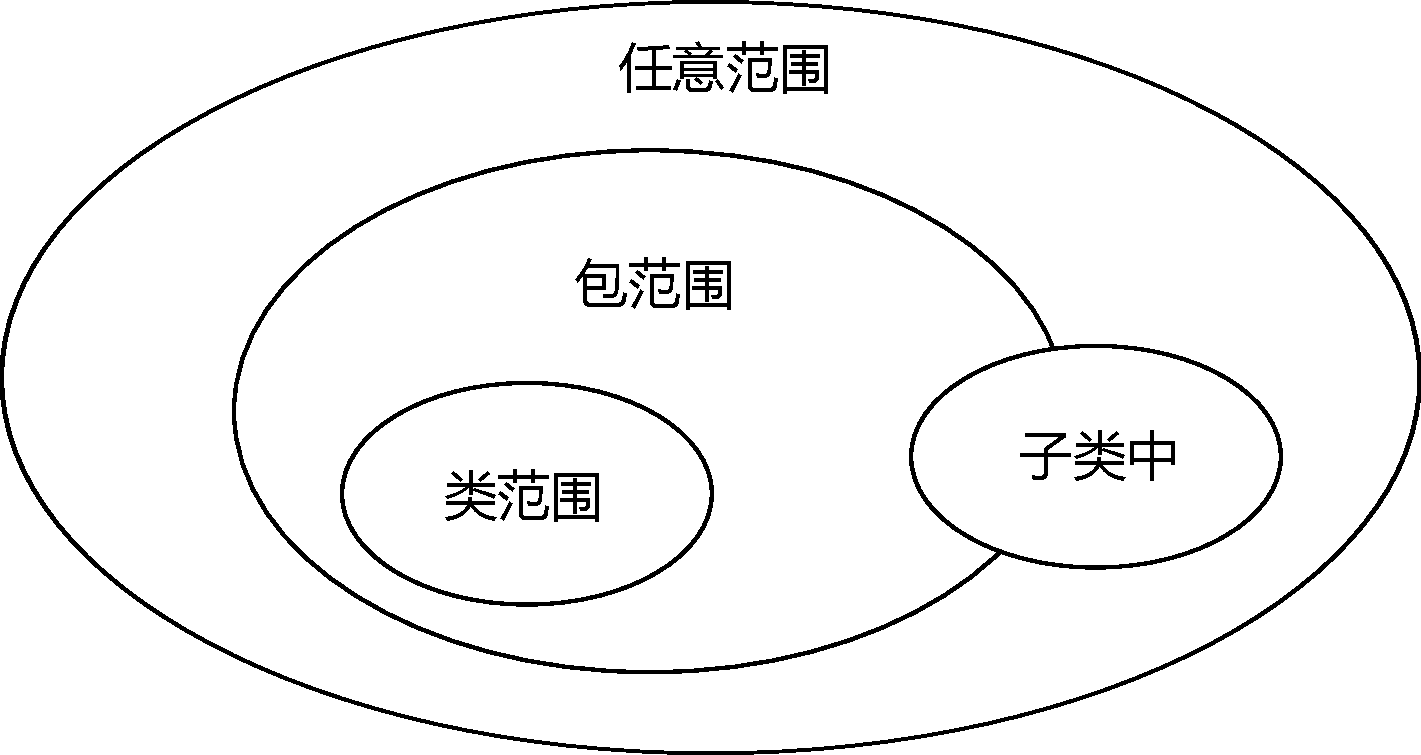
\includegraphics[width=0.6\textwidth]{images/Advanced-object-oriented-programming-1/fig-java-access-control.pdf}
\caption{Java访问控制}
\label{fig:java-access-control}
\end{figure}


\subsection{访问控制protected}

\samplecode{A.java}

\begin{javaCode}
  package p1;
  public class A {
    public int m = 5;
    protected int n = 6;
  }
\end{javaCode}

\samplecode{B.java}
\begin{javaCode}
  package p2;
  import p1.A;
  public class B extends A {
    public void mb() {
      m = m + 1;
      n = n * 2;
    }
    
    public static void main(String[] args) {
      B b = new B();
      b.m = 7;  // 合法
      b.n = 8;   // 合法
      A a = new A();
      a.m = 9 // 合法
      a.n = 10 // 非法
    }
  }
\end{javaCode}

\section{同名问题}

\subsection{方法重写}

在子类中可以根据需要对从父类中继承来的方法进行重新定义,此称方法重写(Override)或覆盖。

\begin{itemize}
\item 重写方法必须和被重写方法具有相同的方法名称、参数列表和返回值类型;
\item 重写方法不能使用比被重写方法更严格的访问权限;
\item 重写方法不允许声明抛出比被重写方法范围更大的异常类型。
\end{itemize}

\samplecode{方法重写示例:Person.java}
\begin{javaCode}
  public class Person {
    String name;
    int age;
    public String getInfo() {
      return "Name:"+ name + "\t" +"age:"+ age;
    }
  }
\end{javaCode}

\samplecode{方法重写示例:Student.java}

\begin{javaCode}
  public class Student extends Person {
    private String school;
    public void setSchool(String scholl) {
      this.school = school;
    }
    public String getSchool(){
      return school;
    }
    public String getInfo() {
      return "Name:"+ name + "\tAge:"+ age + "\tSchool:" + school;
    }
  }
\end{javaCode}

\samplecode{方法重写示例:Parent.java}
\begin{javaCode}
  public class Parent {
    public void method1() {...}
  }
\end{javaCode}

\samplecode{方法重写示例:Child.java}

\begin{javaCode}
  public class Child extends Parent {
    private void method1() {} //非法,权限更严格
  }
\end{javaCode}

\subsection{同名属性}

\begin{javaCode}
  public class Person {
    int age = 5;
    public int getAge() {
      return age;
    }
    public int getInfo() {
      return age;
    }
  }
\end{javaCode}

\begin{javaCode}
  public class Student extends Person {
    int age = 6;
    public int getAge() {
      return age;
    }
  }
\end{javaCode}

\begin{javaCode}
  public class Test {
    public static void main(String args[]) {
      Person p = new Person();
      System.out.println(p.getAge());
      Student s = new Student();
      System.out.println(s.age);
      System.out.println(s.getAge());
      System.out.println(s.getInfo());
    }
  }
\end{javaCode}

上述程序的输出结果为:

\begin{stdoutCode}
  5
  6
  6
  5
\end{stdoutCode}

\descript{对上述Student对象同名属性的几点说明}

\begin{enumerate}
\item 以“对象名.属性名”方式直接访问时,使用的是子类中添加的属性age;
\item 调用子类添加或者重写的方法时,方法中使用的是子类定义的属性age;
\item 调用父类中定义的方法时,方法中使用的是父类中的属性age;
\item 可以理解为“{\bf\Blue 层次优先~就近原则}”,在哪个层次中的代码,就优先使用该层次类中
  定义的属性。不提倡使用同名属性。
\end{enumerate}

\subsection{关键字super} 

在存在命名冲突(子类中存在方法重写或添加同名属性)的情况下,子类中的代码将自动使用子类中
的同名属性或重写后的方法。当然也可以在子类中{\Red 使用关键字super引用父类中的成分}:

\subsubsection{访问父类中定义的属性}

\begin{javaCode}
  super.<属性名>  
\end{javaCode}

\subsubsection{调用父类中定义的成员方法}

\begin{javaCode}
  super.<方法名>(<实参列表>)
\end{javaCode}

\subsubsection{子类构造方法中调用父类的构造方法}

\begin{javaCode}
  super(<实参列表>)  
\end{javaCode}

super的追溯不仅限于直接父类,而是先从直接父类开始查找,如果找不到则逐层
上溯,一旦在某个层次父类中找到匹配成员即停止追溯并使用该成员。

\samplecode{super用法示例A}

\begin{javaCode}
  class Animal {
    protected int i = 1;   //用于测试同名属性,无现实含义
  }

  class Person extends Animal {
    protected int i = 2;     //用于测试同名属性,无现实含义
    private String name = "Tom";
    private int age = 9;
    public String getInfo() {
      return "Name:" + name + "\tAge:" + age;
    }
    public void testI() {
      System.out.println(super.i);
      System.out.println(i);
    }
  }
\end{javaCode}

\samplecode{super用法示例B}

\begin{javaCode}
  class Student extends Person {
    private int i = 3;
    private String school = "THU";
    public String getInfo() {       //重写方法
      return super.getInfo() + "\tSchool:" + school;
    }
    public void testI() {       //重写方法
      System.out.println(super.i);
      System.out.println(i);
    }
  }
  public class Test {
    public static void main(String args[]) {
      Person p = new Person();
      System.out.println(p.getInfo());
      p.testI();
      Student s = new Student();
      System.out.println(s.getInfo());
      s.testI();
    }
  }
\end{javaCode}

上述代码的输出结果为:

\begin{stdoutCode}
  Name:Tom Age:9
  1
  2
  Name:Tom Age:9 School:THU
  2
  3  
\end{stdoutCode}

\subsection{关键字this}

在Java方法中,不但可以直接使用方法的局部变量,也可以使用调用该方法的对
象。为解决可能出现的命名冲突,Java语言引入this关键字来标明方法的当前对
象。分为两种情况:

\begin{itemize}
\item 在普通方法中,关键字this代表方法的调用者,即本次调用了该方法的对象;
\item 在构造方法中,关键字this代表该方法本次运行所创建的那个新对象。
\end{itemize}

this作为一个特殊的引用类型变量,可以通过“{\Red this.成员}”的方式访问
其引用的当前对象的属性和方法。

\samplecode{this用法示例}
\begin{javaCode}
  public class MyDate {
    private int day = 17;
    private int month = 2;

    public MyDate(int day, int month) {
      this.day = day; // A
      this.month = month;
    }
    ... // Some methods 

    public void setAll(int day, int month) {
      this.setMonth(month); // B
      this.setDay(day);
    }
  }
\end{javaCode}

\descript{关于this的归纳说明}

\begin{enumerate}
\item 在Java方法中直接给出变量名而不是“对象名.变量名”的方式访问一个变
  量,系统首先尝试作为局部变量来处理;如果方法中不存在该名字的局部变量,
  才会到方法当前对象的成员变量中查找。
\item 在Java方法中直接调用一个方法而不指定其调用者时,则默认调用者为当
  前对象this。
\end{enumerate}

\newpage
\section*{实验设计}
\sline

% Week 03 %%
\chapter{Java 面向对象编程进阶 B}
\label{chp:Advanced-object-oriented-programming-2}

\section*{基本信息}
\sline
\begin{description}
\item[课程名称:] Java应用与开发
\item[授课教师:] 王晓东
\item[授课时间:] 第二周(根据校历,本周有两次课)
\item[参考教材:] 本课程参考教材及资料如下:
  \begin{itemize}
  \item 陈国君主编,Java程序设计基础(第5版),清华大学出版社,2015.5
  \item Bruce Eckel, Thinking in Java (3rd)
  \end{itemize}
\end{description}

\section*{教学目标}

\sline

\begin{enumerate}
\item 理解多态和虚方法调用的概念,掌握其用法
\item 掌握方法重载的方法
\item 掌握static属性、方法和初始化块的用法
\item 了解设计模式,掌握单例设计模式
\item 掌握final关键字的概念和使用方法
\end{enumerate}  

\section*{授课方式}

\sline
\begin{description}
\item[理论课:] 多媒体教学、程序演示
\item[实验课:] 上机编程
\end{description}

\newpage
\section*{教学内容}
\sline

%%%%%%%%%%%%%%%%%%%%%%%%%%%%%%%%%%%%%%%%%%%%%%%%%%%%%%%%%%%%%%
\section{多态性}

\subsection{多态的概念}

在Java中,子类的对象可以替代父类的对象使用称为{\hei 多态}。Java引用变量
与所引用对象间的类型匹配关系如下:

\begin{itemize}
\item 一个对象只能属于一种确定的数据类型,该类型自对象创建直至销毁不能
  改变。
\item 一个引用类型变量可能引用(指向)多种不同类型的对象——既可以引用其
  声明类型的对象,也可以引用其声明类型的子类的对象。
  \begin{javaCode}
    Person p = new Student(); //Student 是 Person 的子类  
  \end{javaCode}
\end{itemize}

\begin{figure}[htb]
  \centering
  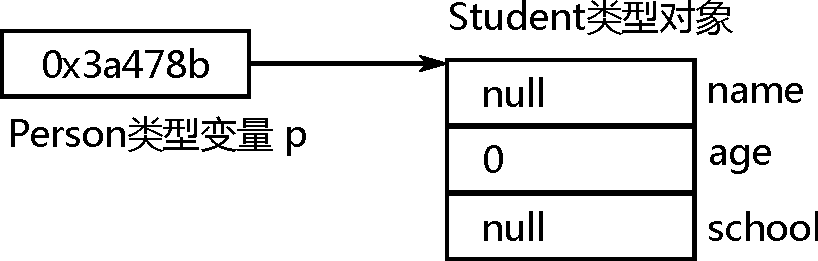
\includegraphics[width=0.6\textwidth]{images/Advanced-object-oriented-programming-2/fig-poly.pdf}
  \caption{Java多态}
  \label{fig:poly}
\end{figure}

多态性同样适用与引用类型数组元素。

\begin{javaCode}
  Person[] p = new Person[3]; 
  p[0] = new Student(); // 假设 Student 类继承了 Person 类
  p[1] = new Person();
  p[2] = new Graduate(); //假设 Graduate 类继承了 Student 类
\end{javaCode}

一个引用类型变量如果声明为父类的类型,但实际引用的是子类对象,该变量则不能再访问子类
中添加的属性和方法,这体现了父类引用对子类对象的能力屏蔽性。

\begin{javaCode}
  Student m = new Student();
  m.setSchool("ouc"); // 合法
  Person e = new Student();
  e.setSchool("ouc"); // 非法
\end{javaCode}

\subsection{多态用法示例}

\samp{Person.java}

\begin{javaCode}
  public class Person {...}
\end{javaCode}

\samp{Student.java}

\begin{javaCode}
  public class Student extends Person {
    private String school;

    public void setSchool(String school) {
      this.school = school;
    }

    public String getSchool() {
      return school;
    }

    @Override
    public String getInfo() {
      return super.getInfo() + "\tSchool: " + school;
    }
  }
\end{javaCode}

\samp{PolymorphismSample.java}

\begin{javaCode}
  public class PolymorphismSample {
    public void show(Person p) {
      System.out.println(p.getInfo());
    }
    
    public static void main(String[] args) {
      PolymorphismSample ps = new PolymorphismSample();
      Person p = new Person();
      ps.show(p);
      Student s = new Student();
      ps.show(s);
    }
  }
\end{javaCode}

\notice{多态提升方法通用性}

以上代码中,show()方法既可以处理Person类型的数据,又可以处理Student类型
的数据,乃至未来定义的任何Person子类类型的数据,即不必为相关的每种类型
单独声明一个处理方法,提高了代码的通用性。

\subsection{虚方法调用}

思考:一个引用类型的变量如果声明为父类的类型,但实际引用的是子类对象,
则该变量就不能再访问子类中添加的属性和方法。但如果此时调用的是父类中声
明过、且在子类中重写过的方法,情况如何?

补充代码。

\subsection{对象造型}

引用类型数据值之间的强制类型转换称为{\hei 造型(Casting)}。造型以下几种情况需要注意:

\begin{enumerate}
\item 从子类到父类的类型转换可以自动进行。
  \begin{javaCode}
    Person p = new Student();    
  \end{javaCode}
\item 在多态的情况下,有时我们可能需要恢复一个对象的本来面目,以发挥其
  全部潜力。从父类到子类的类型转换必须通过造型实现。
  \begin{javaCode}
    Person p1 = new Student();  
    Student s1 = (Student)p1;   // 合法
    Person p2 = new Person();   
    Student s2 = (Student)p2;  // 非法  
  \end{javaCode}
\item 无继承关系的引用类型间的转换是非法的。
  \begin{javaCode}
    String s = "Hello World!";
    Person p = (Person)s; // 非法  
  \end{javaCode}
\end{enumerate}

\subsection{instanceof运算符}

如果运算符instanceof左侧的变量当前时刻所引用的对象的{\hei\Red 真正类型}是
其右侧给出的类型{\Blue 或者是其子类},则整个表达式的结果为true。

\begin{javaCode}
class Person { --- }
class Student extends Person { --- }

public class Tool {
  public void distribute(Person p) {
    if (p instanceof Student) {
      System.out.println("处理 Student 类型及其子类类型对象");
    } else {
      System.out.println("处理 Person 类型及其子类类型对象");
    }
  }
}
\end{javaCode}

\begin{javaCode}
public class Test() {
  public static void main(String[] args) {
    Tool t = new Tool();
    Student s = new Student();
    t.distribute(t);
  }
}
\end{javaCode}

\subsection{虚方法调用和造型}

\codeset{package sample.oop.poly}

\begin{itemize}\small
\item VirtualMethodSample.java
\item Person.java
\item Student.java
\end{itemize}
  
强调以下与虚方法调用和造型相关的重点:
  
\begin{itemize}
\item 系统根据运行时对象的真正类型来确定具体调用哪一个方法,这一机制被称为
  {\hei\Blue 虚方法调用}。
\item 造型是引用类型数据值之间的强制类型转换。
\item instanceof运算符判断的是当前所引用对象的真正类型是什么,而不是声明的引用类型。
\end{itemize}

\section{方法重载}

\subsection{方法重载的概念}

在一个类中存在多个同名方法的情况称为{\hei 方法重载(Overload)}。Java对方法重载有以下要求:

\begin{itemize}
\item 重载方法参数列表必须不同。
\item 重载既可以用于普通方法,也可以用于构造方法。
\end{itemize}

\codeset{sample.oop.MethodOverloadSample.java}


\subsection{调用重载的构造方法}
  
\subsubsection{使用this调用当前类中重载构造方法}

可以在构造方法的第一行使用关键字this调用其它(重载的)构造方法。

\begin{javaCode}
  public class Person {
    ...
    public Person(String name,int age) {
      this.name = name;
      this.age = age;
    }
    public Person(String name) {
      this(name, 18);
    }
    ...
  }
\end{javaCode}

\notice{注意}

关键字this的此种用法只能用在构造方法中,且this()语句如果出
现必须位于方法体中代码的第一行。

\subsubsection{使用super调用父类构造方法}

\samp{Person.java}

\begin{javaCode}
  public class Person {
    ... (此处没有无参构造方法)
    public Person(String name, int age) {
      this.name = name;
      this.age = age;
    }
    ...
  }  
\end{javaCode}

\samp{Student.java}

\begin{javaCode}
  public class Student extends Person {
    private String school;
    public Student(String name, int age, String school) {
      super(name, age); // 显式调用父类有参构造方法
      this.school = school;
    }
    public Student(String school) { //编译出错
      // super(); // 隐式调用父类有参构造方法,则自动调用父类无参构造方法
      this.school = school;
    }
  }
\end{javaCode}

\notice{上述代码为什么会编译出错?}

{\Blue\hei 在Java类的构造方法中一定直接或间接地调用了其父类的构造方法(Object类除外)。}

\begin{enumerate}
\item 在子类的构造方法中可使用super语句调用父类的构造方法,其格式为super(<实参列表>)。
\item 如果子类的构造方法中既没有显式地调用父类构造方法,也没有使用this关键字调用同一个类
  的其他重载构造方法,则系统会默认调用父类无参数的构造方法,其格式为super()。
\item 如果子类构造方法中既未显式调用父类构造方法,而父类中又没有无参的构造方法,则编译出
  错。
\end{enumerate}

\codeset{sample.oop.ConstructorOverloadSample.java}
  


\subsection{对象构造/初始化细节}

\begin{description}
\item [第一阶段] 为新建对象的实例变量分配存储空间并进行默认初始化。
\item [第二阶段] 按下述步骤继续初始化实例变量:
  \begin{enumerate}
  \item 绑定构造方法参数;
  \item 如有this()调用,则调用相应的重载构造方法然后跳转到步骤5;
  \item 显式或隐式追溯调用父类的构造方法(Object类除外);
  \item 进行实例变量的显式初始化操作;
  \item 执行当前构造方法的方法体中其余的语句。 
  \end{enumerate}
\end{description}

\section{关键字static}

在Java类中声明{\hei\Red 属性、方法和内部类}时,可使用关键字static作为修饰符。

\begin{itemize}
\item static标记的属性或方法由整个类(所有实例)共享,如访问控制权限
  允许,可不必创建该类对象而直接用类名加“.”调用。
\item static成员也称{\hei\Blue “类成员”或“静态成员”},如“类属
  性”、“类变量”、“类方法”和“静态方法”等。
\end{itemize}

\subsection{static属性和方法}

\subsubsection{static属性}

\begin{itemize}
\item static属性由其所在类(包括该类所有的实例)共享。
\item 非static属性则必须依赖具体/特定的对象(实例)而存在。
\end{itemize}

\subsubsection{static方法}

要在static方法中调用其所在类的非static成员,应首先创建一个该类的对象,
通过该对象来访问其非static成员。

\codeset{sample.oop.StaticMemberAndMethodSample.java}


\subsection{初始化块}

\subsubsection{static初始化块}

在类的定义体中,方法的外部可包含static语句块,{\Red static块仅在其所属
  的类被载入时执行一次},通常用于初始化化static(类)属性。

\subsubsection{非static初始化块}

非static的初始化块在创建对象时被自动调用。

\codeset{sample.oop.StaticInitBlockSample.java}

\subsection{静态导入}

静态导入用于在一个类中导入其他类或接口中的static成员,语法格式如下:

\begin{javaCode}
  import static <包路径>.<类名>.*

  import static <包路径>.<类名>.<静态成员名>
\end{javaCode}

\samp{静态导入应用示例}

\begin{javaCode}
import static java.lang.Math.*;
public class Test {
  public static void main(String[] args) {
    double d = sin(PI * 0.45);
    System.out.println(d);
  }
}
\end{javaCode}

\subsection{Singleton设计模式}

所谓“模式”就是被验证为有效的常规问题的典型解决方案。{\hei 设计模式
  (Design Pattern)}在面向对象分析设计和软件开发中占有重要地位。好的设
计模式可以使我们更加方便的重用已有的成功设计和体系结构,极大的提高代码
的重用性和可维护性。

经典设计模式分类主要分为以下三大类:

\begin{description}
\item[创建型模式] 涉及对象的实例化,特点是不让用户代码依赖于对象的创建或排列方式,避免用户直接使用new创建对象。\\
  {\Red\kai 工厂方法模式、抽象工厂方法模式、生成器模式、原型模式和单例
    模式}
\item[行为型模式] 涉及怎样合理的设计对象之间的交互通信,以及合理为对象分配职责,让设计富有弹性、易维护、易复用。\\
  {\Blue\kai 责任链模式、命令模式、解释器模式、迭代器模式、中介者模式、
    备忘录模式、观察者模式、状态模式、策略模式、模板方法模式和访问者模
    式}
\item[结构型模式] 涉及如何组合类和对象以形成更大的结构,和类有关的结构型模式涉及如何合理使用继承机制,和对象有关的结构型模式涉及如何合理的使用对象组合机制。\\
  {\Mage\kai 适配器模式、组合模式、代理模式、享元模式、外观模式、桥接模
    式和装饰模式}
\end{description}


Singleton设计模式也称“单子模式”或“单例模式”。

\notice{采用调试方式讲解示例代码}

Singleton代码的特点包括以下几个方面:

\begin{enumerate}
\item 使用静态属性onlyone来引用一个“全局性”的Single实例。
\item 将构造方法设置为private的,这样在外界将不能再使用new关键字来创建该类的新实例。
\item 提供public static的方法getSingle()以使外界能够获取该类的实例,达到全局可见的效果。
\end{enumerate}

在任何使用到Single类的Java程序中(这里指的是一次运行中),需要确保只有
一个Single类的实例存在(如Web应用ServletContext全局上下文对象),则使用
该模式。

\section{关键字final}

在声明Java类、变量和方法时可以使用关键字final来修饰,以使其具有“终态”的特性:

\begin{enumerate}\kai
\item final标记的类不能被继承;
\item final标记的方法不能被子类重写;
\item final标记的变量(成员变量或局部变量)即成为常量,只能赋值一次;
\item final标记的成员变量必须在声明的同时或在每个构造方法中显式赋值,然后才能使用;
\item final不允许用于修饰构造方法、抽象类以及抽象方法。
\end{enumerate}

关键字final应用举例如下:

\begin{javaCode}
public final class Test {
  public static int totalNumber = 5;
  public final int id;
  public Test() {
    id = ++totalNumber; // 赋值一次
  }
  public static void main(String[] args) {
    Test t = new Test();
    System.out.println(t.id);
    final int i = 10;
    final int j;
    j = 20;
    j = 30;  // 非法
  }
}
\end{javaCode}

\section{课后习题}

\tta{简答题}
\begin{enumerate}
\item 为什么建议Java类需要编写无参构造方法,哪怕该方法什么都没做?
\item 关键字static都可以用来修饰Java类的那些成员?
\end{enumerate}

\tta{小编程}
\begin{enumerate}
\item 练习本节中所有示例代码,理解并掌握其用法。
\item 自行调试单例设计模式程序,学习Eclipse的Debug方法,练习断点、单
  步执行、跟进方法等操作,查看内存变化。
\end{enumerate}
\chapter{Java内存模型与分配机制}
\label{chp:Java-memory-allocation}

\section*{基本信息}
\sline
\begin{description}
\item[课程名称:] Java应用与开发
\item[授课教师:] 王晓东
\item[授课时间:] 第二周(根据校历,本周有两次课)
\item[参考教材:] 本课程参考教材及资料如下:
  \begin{itemize}
  \item 陈国君主编,Java程序设计基础(第5版),清华大学出版社,2015.5
  \item Bruce Eckel, Thinking in Java (3rd)
  \end{itemize}
\end{description}

\section*{教学目标}

\sline

\begin{enumerate}
\item 理解JVM内存模型,掌握JVM内存构成
\item 理解Java程序的运行过程,学会通过调试模式观察内存的变化
\item 了解Java内存管理,认识垃圾回收
\item 建立编程时高效利用内存、避免内存溢出的理念
\end{enumerate}  

\section*{授课方式}

\sline
\begin{description}
\item[理论课:] 多媒体教学、程序演示
\item[实验课:] 上机编程
\end{description}

\newpage
\section*{教学内容}
\sline

%%%%%%%%%%%%%%%%%%%%%%%%%%%%%%%%%%%%%%%%%%%%%%%%%%%%%%%%%%%%%%
\section{Java内存模型}

\subsection{Java虚拟机(Java Virtual Machine, JVM)}

Java虚拟机的架构如图\ref{fig:jvm-arch}所示。

\begin{figure}[htb]
  \centering
  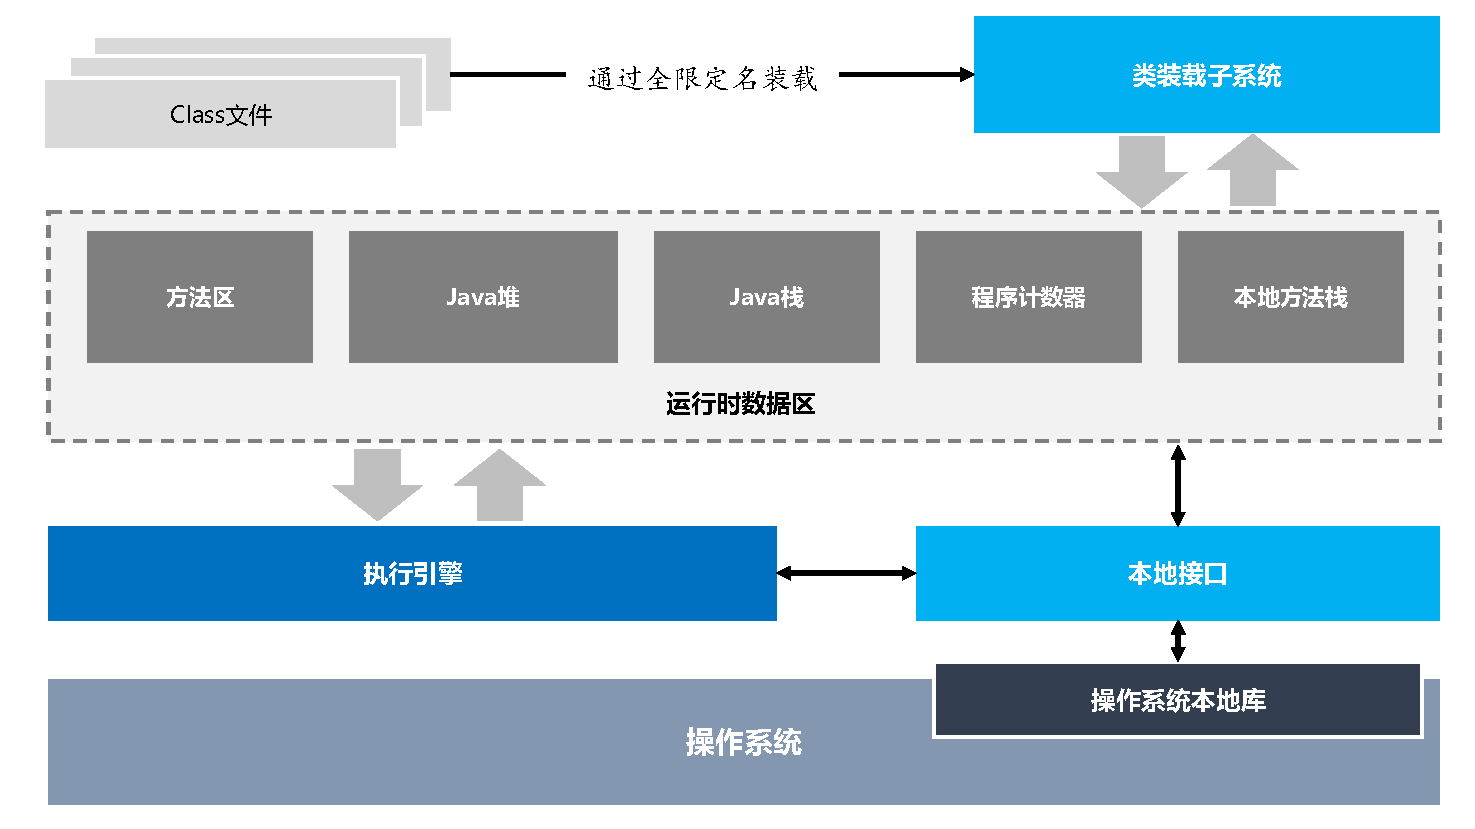
\includegraphics[width=\textwidth]{images/Java-memory-allocation/fig-jvm-arch.pdf}
  \caption{Java虚拟机架构}
  \label{fig:jvm-arch}
\end{figure}

\begin{itemize}
\item Java程序运行在JVM上,JVM是程序与操作系统之间的桥梁。
\item JVM实现了Java的平台无关性。
\item JVM是内存分配的前提。
\end{itemize}

\subsection{JVM内存模型}

\begin{figure}[htb]
  \centering
  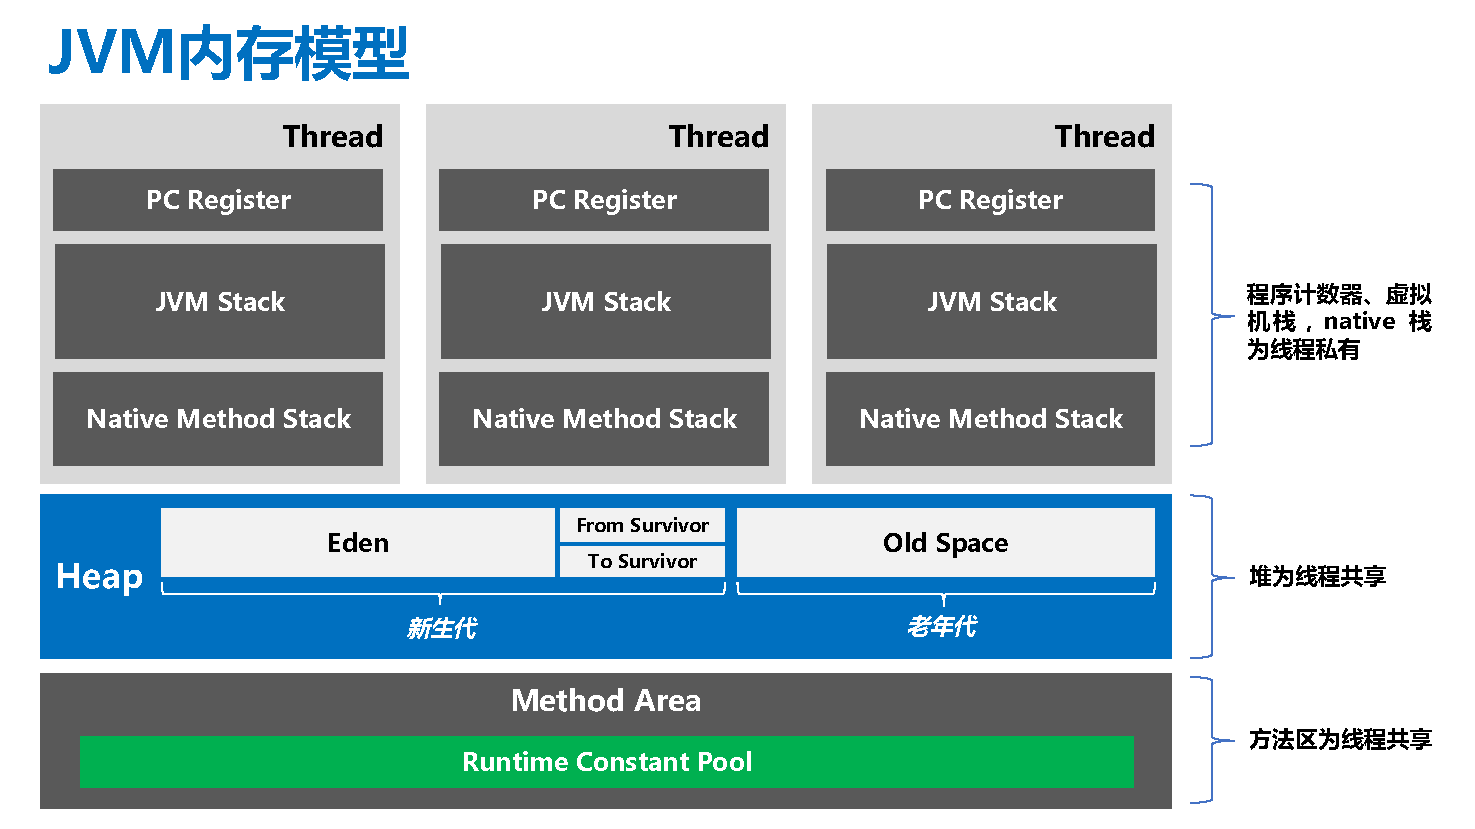
\includegraphics[width=\textwidth]{images/Java-memory-allocation/fig-java-memory-arch.pdf}
  \caption{JVM内存模型}
  \label{fig:java-memory-arch}
\end{figure}

Java程序运行过程会涉及的内存区域包括:

\begin{description}
\item[程序计数器] 当前线程执行的字节码的行号指示器。
\item[栈] 保存局部变量的值,包括:用来保存基本数据类型的值;保存类的实
  例,即堆区对象的引用(指针),也可以用来保存加载方法时的帧。(Stack)
\item[堆] 用来存放动态产生的数据,如new出来的对象和数组\footnote{注意创
    建出来的对象只包含属于各自的成员变量,并不包括成员方法。因为同一个
    类的对象拥有各自的成员变量,存储在各自的堆内存中,但是他们共享该类
    的方法,并不是每创建一个对象就把成员方法复制一次。}。(Heap)
\item[常量池] JVM为每个已加载的类型维护一个常量池,常量池就是这个类型用
  到的常量的一个有序集合。包括直接常量(基本类型、String)和对其他类型、
  方法、字段的符号引用。池中的数据和数组一样通过索引访问,常量池
  在Java程序的动态链接中起了核心作用。(Perm)
\item[代码段] 存放从硬盘上读取的源程序代码。(Perm)
\item[数据段] 存放static定义的静态成员。{\Red (Perm)} 
\end{description}

\section{Java程序内存运行分析}

\subsection{预备知识和所用讲解程序}

\begin{enumerate}
\item 一个Java文件,只要有main入口方法,即可认为这是一个Java程序,可以
  单独编译运行。
\item 无论是普通类型的变量还是引用类型的变量(俗称实例),都可以作为局
  部变量,他们都可以出现在栈中。
\item 普通类型的变量在栈中直接保存它所对应的值,而引用类型的变量保存的
  是一个指向堆区的指针。通过这个指针,就可以找到这个实例在堆区对应的对
  象。因此,{\hei\Red 普通类型变量只在栈区占用一块内存,而引用类型变量
    要在栈区和堆区各占一块内存}。
\end{enumerate}

\samp{Test.java}

\begin{javaCode}
  public class Test {
    public static void main(String[] args) {
      Test test = new Test(); //1
      int data = 9; //2
      BirthDate d1 = new BirthDate(22, 12, 1982); //3
      BirthDate d2 = new BirthDate(10, 10, 1958); //4
      test.m1(data); //5
      test.m2(d1); //7
      test.m3(d2);
    }

    public void m1(int i) {
      i = 1234; //6
    }
    public void m2(BirthDate b) {
      b = new BirthDate(15, 6, 2010); //8
    }
    public void m3(BirthDate b) {
      b.setDay(18);
    }
  }
\end{javaCode}

\subsection{程序调用过程}

\subsubsection{程序调用过程(一)}

\begin{itemize}
\item JVM自动寻找main方法,执行第一句代码,创建一个Test类的实例,在栈中分配一块内存,存放
  一个指向堆区对象的指针110925。
\item 创建一个int型的变量data,由于是基本类型,直接在栈中存放data对应的值9。
\item 创建两个BirthDate类的实例d1、d2,在栈中分别存放了对应的指针指向各自的对象。它们在实
  例化时调用了有参数的构造方法,因此对象中有自定义初始值。
\end{itemize}

\subsubsection{程序调用过程(二)}

\begin{itemize}
\item 调用test对象的m1方法,以data为参数。JVM读取这段代码时,检测到i是局部变量,则会把i放
  在栈中,并且把data的值赋给i。
\end{itemize}

\subsubsection{程序调用过程(三)}

\begin{itemize}
\item 把1234赋值给i。
\end{itemize}

\subsubsection{程序调用过程(四)}

\begin{itemize}
\item m1方法执行完毕,立即释放局部变量i所占用的栈空间。
\end{itemize}

\subsubsection{程序调用过程(五)}

\begin{itemize}
\item 调用test对象的m2方法,以实例d1为参数。JVM检测到m2方法中的b参数为
  局部变量,立即加入到栈中,由于是引用类型的变量,所以b中保存的是d1中的
  指针,此时b和d1指向同一个堆中的对象。在b和d1之间传递是指针。
\end{itemize}

\subsubsection{程序调用过程(六)}

\begin{itemize}
\item m2方法中又实例化了一个BirthDate对象,并且赋给b。在内部执行过程是:
  在堆区new了一个对象,并且把该对象的指针保存在栈中b对应空间,此时实
  例b不再指向实例d1所指向的对象,但是实例d1所指向的对象并无变化,未
  对d1造成任何影响。
\end{itemize}

\subsubsection{程序调用过程(七)}

\begin{itemize}
\item m2方法执行完毕,立即释放局部引用变量b所占的栈空间,注意只是释放了
  栈空间,堆空间要等待自动回收。
\end{itemize}

\subsubsection{程序调用过程(八)}

\begin{itemize}
\item 调用test实例的m3方法,以实例d2为参数。JVM会在栈中为局部引用变
  量b分配空间,并且把d2中的指针存放在b中,此时d2和b指向同一个对象。再调
  用实例b的setDay方法,其实就是调用d2指向的对象的setDay方法。
\item 调用实例b的setDay方法会影响d2,因为二者指向的是同一个对象。
\item m3方法执行完毕,立即释放局部引用变量b。
\end{itemize}

\begin{figure}[htb]
  \begin{minipage}[t]{0.5\linewidth}
    \centering
    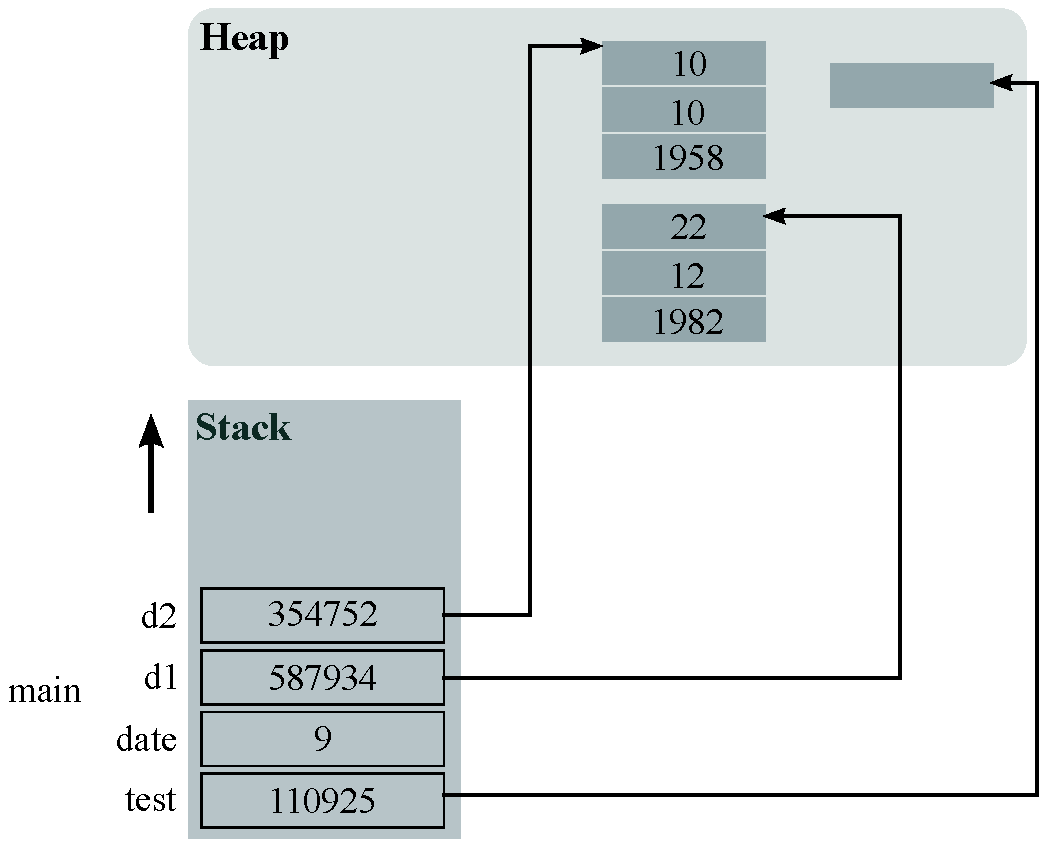
\includegraphics[width=\textwidth]{images/Java-memory-allocation/fig01.pdf}
  \end{minipage}%
  \begin{minipage}[t]{0.5\linewidth}
    \centering
    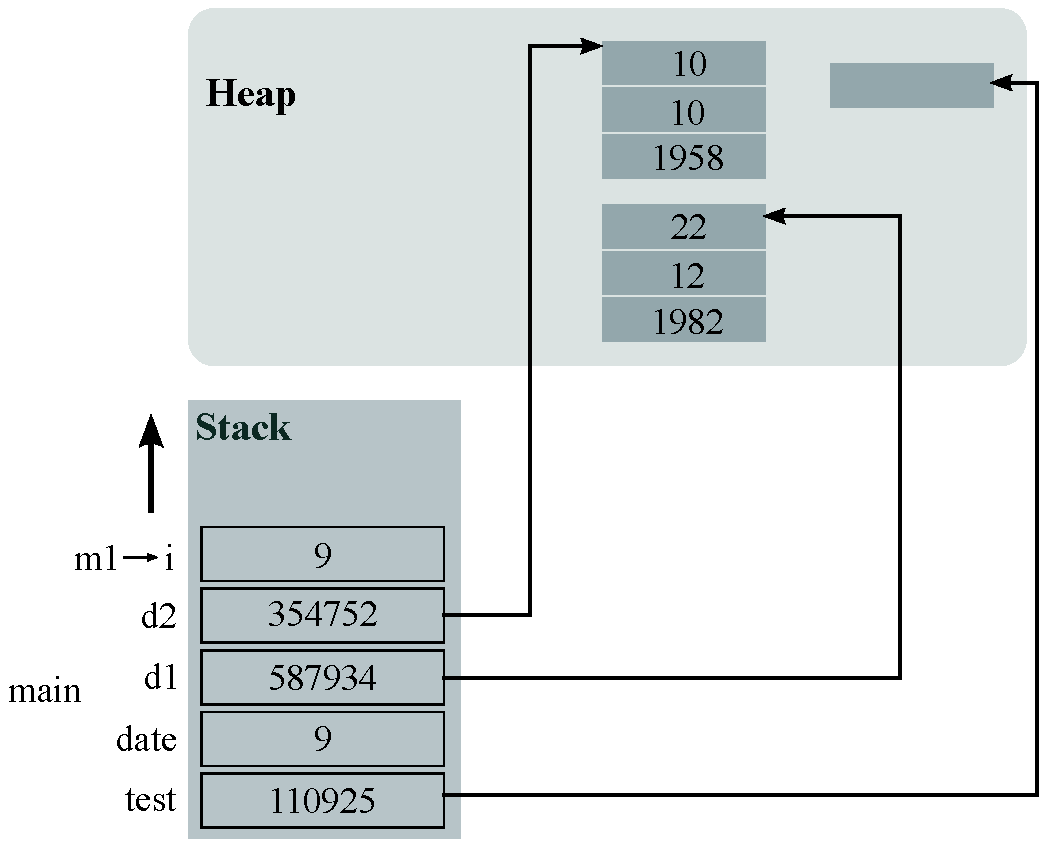
\includegraphics[width=\textwidth]{images/Java-memory-allocation/fig02.pdf}
  \end{minipage}
\end{figure}

\begin{figure}[htb]
  \begin{minipage}[t]{0.5\linewidth}
    \centering
    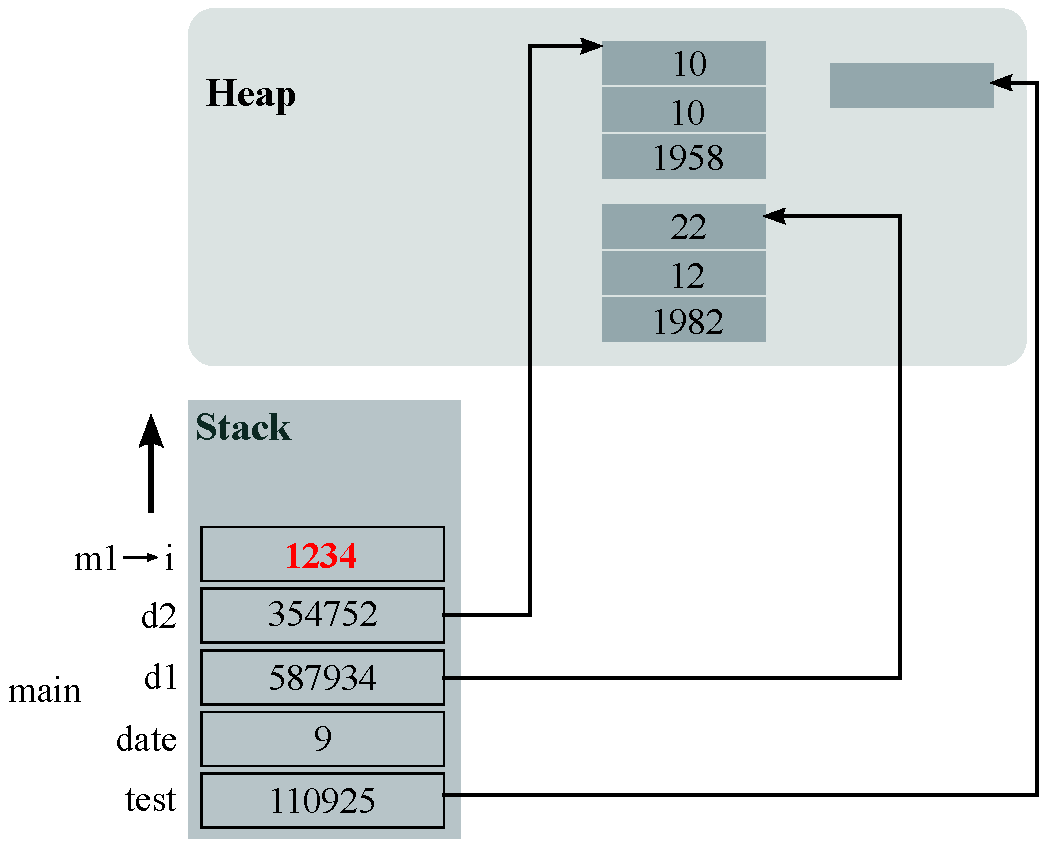
\includegraphics[width=\textwidth]{images/Java-memory-allocation/fig03.pdf}
  \end{minipage}%
  \begin{minipage}[t]{0.5\linewidth}
    \centering
    \includegraphics[width=\textwidth]{images/Java-memory-allocation/fig04.pdf}
  \end{minipage}
\end{figure}

\begin{figure}[htb]
  \begin{minipage}[t]{0.5\linewidth}
    \centering
    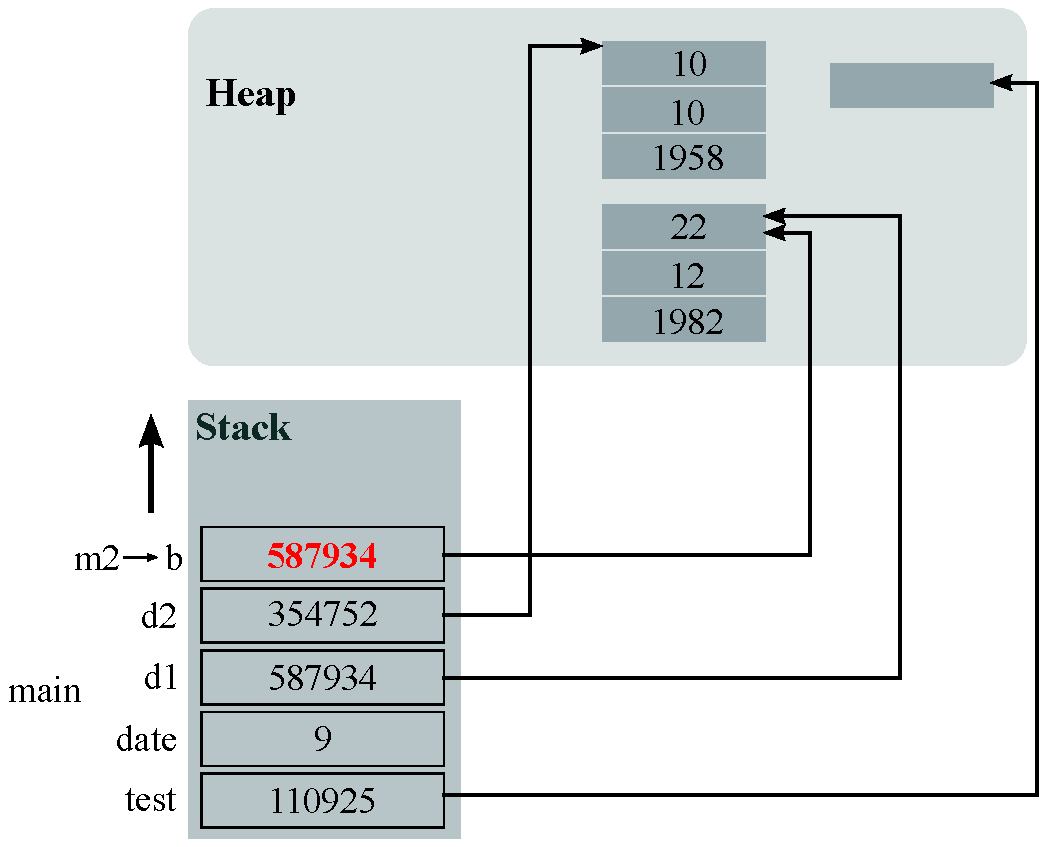
\includegraphics[width=\textwidth]{images/Java-memory-allocation/fig05.pdf}
  \end{minipage}%
  \begin{minipage}[t]{0.5\linewidth}
    \centering
    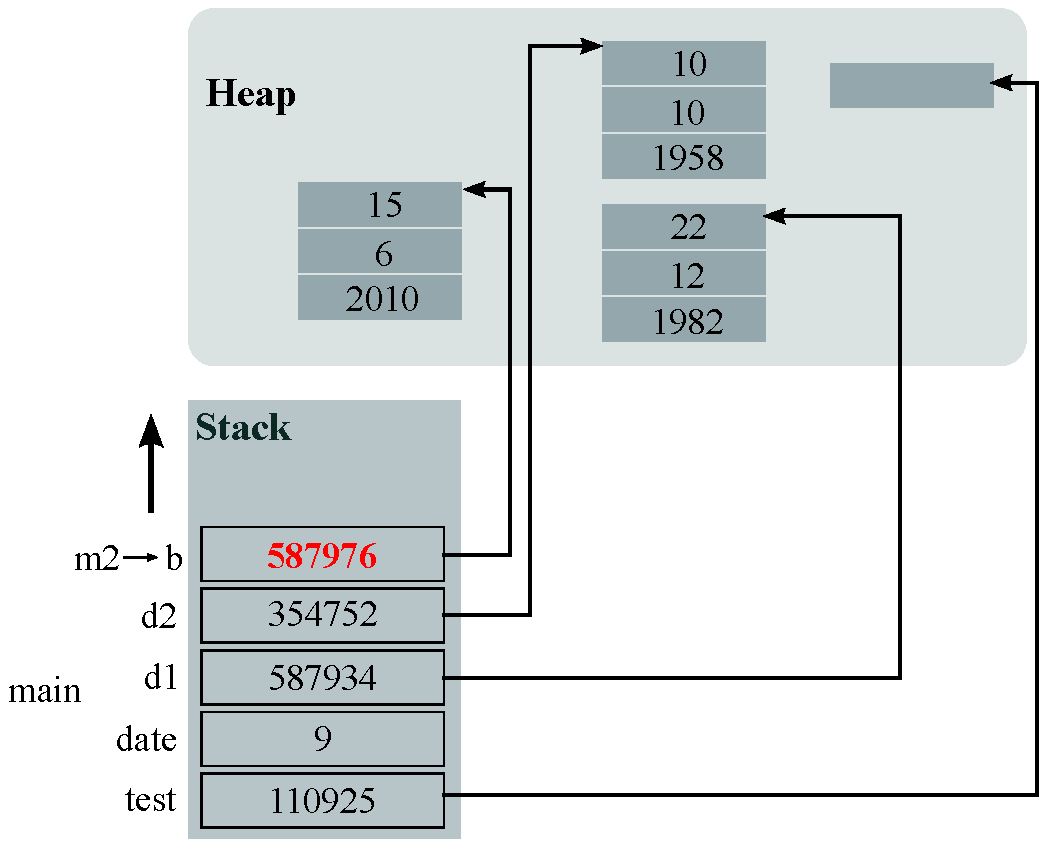
\includegraphics[width=\textwidth]{images/Java-memory-allocation/fig06.pdf}
  \end{minipage}
\end{figure}

\subsection{Java程序运行内存分析小结}

\begin{itemize}
\item 基本类型和引用类型,二者作为局部变量时都存放在栈中。
\item 基本类型直接在栈中保存值,引用类型在栈中保存一个指向堆区的指针,
  真正的对象存放在堆中。
\item 作为参数时基本类型就直接传值,引用类型传指针。
\end{itemize}

\notice{注意什么是对象}

\begin{javaCode}
  MyClass a = new MyClass();
\end{javaCode}

此时a是指向对象的指针,而不能说a是对象。指针存储在栈中,对象存储在堆中,
操作实例实际上是通过指针间接操作对象。多个指针可以指向同一个对象。

\begin{itemize}
\item {\hei\Red 栈中的数据和堆中的数据销毁并不是同步的。}方法一旦执行结
    束,栈中的局部变量立即销毁,但是堆中对象不一定销毁。因为可能有其
    他变量也指向了这个对象,直到栈中没有变量指向堆中的对象时,它才销
    毁;而且还不是马上销毁,要等垃圾回收扫描时才可以被销毁。
\item {\hei\Red 栈、堆、代码段、数据段等都是相对于应用程序而言的。}每一
    个应用程序都对应唯一的一个JVM实例,每一个JVM实例都有自己的内存区
    域,互不影响,并且这些内存区域是该JVM实例所有线程共享的。
\end{itemize}

\section{Java内存管理建议}

\subsection{Java垃圾回收机制} 

{\hei\Blue JVM的垃圾回收机制(GC)决定对象是否是垃圾对象,并进行回收。}垃圾回收机制的特点包括:

\begin{itemize}
\item 垃圾内存并不是用完了马上就被释放,所以会产生内存释放不及时的现象,
  从而降低内存的使用效率。而当程序庞大的时候,这种现象更为明显。
\item 垃圾回收工作本身需要消耗资源,同样会产生内存浪费。
\end{itemize}

JVM中的对象生命周期一般分为7个阶段:\ding{182}创建阶段、\ding{183}应用
阶段、\ding{184}不可视阶段、\ding{185}不可到达阶段、\ding{186}可收集阶
段、\ding{187}终结阶段、\ding{188}释放阶段。

Java需要内存管理,在JVM中运行的对象的整个生命周期中,进行人为的内存管理是必要的,主要原因体现在:

\begin{itemize}
\item 虽然JVM已经代替开发者完成了对内存的管理,但是硬件本身的资源是有限的。
\item 如果Java的开发人员不注意内存的使用依然会造成较高的内存消耗,导致性能的降低。
\end{itemize}

\subsection{JVM内存溢出和参数调优}

\notice{当遇到OutOfMemoryError时该如何做?}

\begin{itemize}
\item 常见的OOM(Out Of Memory)内存溢出异常,就是堆内存空间不足以存放
  新对象实例时导致。
\item 永久区内存溢出相对少见,一般是由于需要加载海量的Class数据,超过了
  非堆内存的容量导致。通常出现在Web应用刚刚启动时。因此Web应用推荐使用
  预加载机制,方便在部署时就发现并解决该问题。
 \item 栈内存也会溢出,但是更加少见。
\end{itemize}

对内存溢出的处理方法不外乎这两种:\ding{182} 调整JVM内存配置;\ding{183} 优化代码。

创建阶段的JVM内存配置优化需要关注以下项:

\begin{description}
\item[堆内存优化] 调整JVM启动参数 -Xms -Xmx -XX:newSize -XX:MaxNewSize,
  如调整初始堆内存和最大对内存 -Xms256M -Xmx512M。 或者调整初始New
  Generation的初始内存和最大内存 -XX:newSize=128M -XX:MaxNewSize=128M。
\item[永久区内存优化] 调整PermSize参数,如 -XX:PermSize=256M
  -XX:MaxPermSize=512M。
 \item[栈内存优化] 调整每个线程的栈内存容量,如 -Xss2048K。
\end{description}

\subsection{内存优化的小示例}

\subsubsection{减少无谓的对象引用创建}

\samp{Test 1}

\begin{javaCode}
  for(int i=0; i<10000; i++) {
    Object obj = new Object(); 
  }
\end{javaCode}

\samp{Test 2}

\begin{javaCode}
  Object obj = null; 
  for( int i=0; i<10000; i++) {
    obj = new Object(); 
  }
\end{javaCode}

\descript{内存性能分析}
  
{\small\kai Test 2比Test 1的性能要好。两段程序每次执行for循环都要创建一
  个Object的临时对象,JVM的垃圾回收不会马上销毁但这些临时对象。相对
  于Test 1,Test 2则只在栈内存中保存一份对象的引用,而不必创建大量新临
  时变量,从而降低了内存的使用。}


\subsubsection{不要对同一对象初始化多次}

\begin{javaCode}
  public class A { 
    private Hashtable table = new Hashtable(); 
    public A() { 
      table = new Hashtable();
    }
  }
\end{javaCode}

\descript{内存性能分析}

{\small\kai 上述代码new了两个Hashtable,但是却只使用了一个,另外一个则
  没有被引用而被忽略掉,浪费了内存。并且由于进行了两次new操作,也影响了
  代码的执行速度。另外,不要提前创建对象,尽量在需要的时候创建对象。}

\subsection{对象其他生命周期阶段内存管理}

\begin{description}
\item[应用] 即该对象至少有一个引用在维护它。
\item[不可视] 即超出该变量的作用域。\\{\kai 因为JVM GC并不是马上进行回
    收,而是要判断对象是否被其他引用维护。所以,如果我们在使用完一个对
    象以后对其进行obj = null或者obj.doSomething()操作,将其标记为空,则
    帮助JVM及时发现这个垃圾对象。}
\item[不可到达] 即在JVM中找不到对该对象的直接或者间接的引用。
\item[可收集,终结,释放] 垃圾回收器发现该对象不可到达,finalize方法已
  经被执行,或者对象空间已被重用的时候。
\end{description}

\subsubsection{Java的finalize()方法}

Java所有类都继承自Object类,而finalize()是Object类的一个函数,该函数
在Java中类似于C++的析构函数(仅仅是类似)。一般来说可以通过重
载finalize()的形式来释放类中对象。

\begin{javaCode}
  public class A { 
    public Object a; 

    public A() { 
      a = new Object() ;
    } 
    
    protected void finalize() throws java.lang.Throwable { 
      a = null; // 标记为空,释放对象 
      super.finalize(); // 递归调用超类中的 finalize 方法
    }
  } 
\end{javaCode}

什么时候finalize()被调用由JVM来决定。{\hei\Blue 尽量少用finalize()函
  数,finalize()函数是Java提供给程序员一个释放对象或资源的机会。但它会
  加大GC的工作量,因此尽量少采用finalize方式回收资源。}

\begin{itemize}
\item 一般的,纯Java编写的Class不需要重写finalize()方法,因为Object已
  经实现了一个默认的,除非我们要实现特殊的功能。
\item 用Java以外的代码编写的Class(比如JNI、C++的new方法分配的内存),
  垃圾回收器并不能对这些部分进行正确的回收,这就需要我们覆盖默认的方
  法来实现对这部分内存的正确释放和回收。
\end{itemize}

\newpage
\section*{实验设计}
\sline

% Week 04 %%
%%%%%%%%%%%%%%%%%%%%%%%%%%%%%%%%%%%%%%%%%%%%%%%%%%%%%%%%%%%%%%%%%%%%%%%%%%%%%%%
% Full instructions available at:
% https://github.com/elauksap/focus-beamertheme

\documentclass{beamer}
\usetheme{focus}

% package for font
\usepackage{fontspec}
\defaultfontfeatures{Mapping=tex-text}  %%如果没有它,会有一些 tex 特殊字符无法正常使用,比如连字符。
\usepackage{xunicode,xltxtra}
\usepackage[BoldFont,SlantFont,CJKnumber,CJKchecksingle]{xeCJK}  % \CJKnumber{12345}: 一万二千三百四十五
\usepackage{CJKfntef}  %%实现对汉字加点、下划线等。
\usepackage{pifont}  % \ding{}
% package for math
\usepackage{amsfonts}
% package for graphics
\usepackage[americaninductors,europeanresistors]{circuitikz}
\usepackage{tikz}
\usetikzlibrary{plotmarks}  % placements=positioning
\usepackage{graphicx}  % \includegraphics[]{}
\usepackage{subfigure}  %%图形或表格并排排列
% package for table
\usepackage{colortbl,dcolumn}  %% 彩色表格
\usepackage{multirow}
\usepackage{multicol}
\usepackage{booktabs}
% package for code
\usepackage{fancyvrb}
\usepackage{listings}
% setting for font
%%\setCJKmainfont{Adobe Kaiti Std}
\setCJKmainfont{SimSun}
%%\setCJKmainfont{Microsoft YaHei}
%%\setCJKmainfont{FangSong_GB2312} 
%%\setmainfont{Times New Roman}
%\setsansfont[Mapping=tex-text]{Adobe Song Std}
%如果装了Adobe Acrobat,可在font.conf中配置Adobe字体的路径以使用其中文字体。
%也可直接使用系统中的中文字体如SimSun、SimHei、微软雅黑等。
%原来beamer用的字体是sans family;注意Mapping的大小写,不能写错。
%设置字体时也可以直接用字体名,以下三种方式等同:
%\setromanfont[BoldFont={黑体}]{宋体}
%\setromanfont[BoldFont={SimHei}]{SimSun}
%\setromanfont[BoldFont={"[simhei.ttf]"}]{"[simsun.ttc]"}

% font setting by xeCJK
\setCJKfamilyfont{NSimSun}{NSimSun}
\newcommand{\song}{\CJKfamily{NSimSun}}
%%%\setCJKfamilyfont{AdobeSongStd}{Adobe Song Std}
%%%\newcommand{\AdobeSong}{\CJKfamily{AdobeSongStd}}
\setCJKfamilyfont{FangSong}{FangSong_GB2312}
\newcommand{\fang}{\CJKfamily{FangSong}}
%%%\setCJKfamilyfont{AdobeFangsongStd}{Adobe Fangsong Std}
%%%\newcommand{\AdobeFang}{\CJKfamily{AdobeFangsongStd}}
\setCJKfamilyfont{SimHei}{SimHei}
\newcommand{\hei}{\CJKfamily{SimHei}}
%%%\setCJKfamilyfont{AdobeHeitiStd}{Adobe Heiti Std}
%%%\newcommand{\AdobeHei}{\CJKfamily{AdobeHeitiStd}}
\setCJKfamilyfont{KaiTi}{KaiTi_GB2312}
\newcommand{\kai}{\CJKfamily{KaiTi}}
%%%\setCJKfamilyfont{AdobeKaitiStd}{Adobe Kaiti Std}
\newcommand{\AdobeKai}{\CJKfamily{AdobeKaitiStd}}
\setCJKfamilyfont{LiSu}{LiSu}
\newcommand{\li}{\CJKfamily{LiSu}}
\setCJKfamilyfont{YouYuan}{YouYuan}
\newcommand{\you}{\CJKfamily{YouYuan}}
\setCJKfamilyfont{FZJingLei}{FZJingLeiS-R-GB}
\newcommand{\jinglei}{\CJKfamily{FZJingLei}}
\setCJKfamilyfont{MSYH}{Microsoft YaHei}
\newcommand{\msyh}{\CJKfamily{MSYH}}

\setbeamerfont{frametitle}{series=\Large\hei} % 修改Beamer标题字体

\graphicspath{{figures/}}  %%图片路径
\renewcommand\figurename{图}

% setting for pdf
\hypersetup{% pdfpagemode=FullScreen,%
  pdfauthor={Xiaodong Wang},%
  pdftitle={Title},%
  CJKbookmarks=true,%
  bookmarksnumbered=true,%
  bookmarksopen=false,%
  plainpages=false,%
  colorlinks=true,%
  citecolor=green,%
  filecolor=magenta,%
  linkcolor=blue,%red(default)
  urlcolor=cyan}

% setting for fontspec
\XeTeXlinebreaklocale "zh"  %%表示用中文的断行
\XeTeXlinebreakskip = 0pt plus 1pt minus 0.1pt  %%多一点调整的空间
%%%%%

% 自定义颜色
\def\Red{\color{red}}
\def\Green{\color{green}}
\def\Blue{\color{blue}}
\def\Mage{\color{magenta}}
\def\Cyan{\color{cyan}}
\def\Brown{\color{brown}}
\def\White{\color{white}}
\def\Black{\color{black}}

\lstnewenvironment{xmlCode}[1][]{% for Java
  \lstset{
    basicstyle=\tiny\ttfamily,%
    columns=flexible,%
    framexleftmargin=.7mm, %
    % frame=shadowbox,%
    % rulesepcolor=\color{cyan},%
     frame=single,%
    backgroundcolor=\color{white},%
    xleftmargin=4\fboxsep,%
    xrightmargin=4\fboxsep,%
    numbers=left,numberstyle=\tiny,%
    numberblanklines=false,numbersep=7pt,%
    language=xml, %
    }\lstset{#1}}{}

\lstnewenvironment{javaCode}[1][]{% for Java
  \lstset{
    basicstyle=\tiny\ttfamily,%
    columns=flexible,%
    framexleftmargin=.7mm, %
    frame=shadowbox,%
    rulesepcolor=\color{cyan},%
    % frame=single,%
    backgroundcolor=\color{white},%
    xleftmargin=4\fboxsep,%
    xrightmargin=4\fboxsep,%
    numbers=left,numberstyle=\tiny,%
    numberblanklines=false,numbersep=7pt,%
    language=Java, %
    }\lstset{#1}}{}

\lstnewenvironment{shCode}[1][]{% for Java
  \lstset{
    basicstyle=\scriptsize\ttfamily,%
    columns=flexible,%
    framexleftmargin=.7mm, %
    frame=shadowbox,%
    rulesepcolor=\color{brown},%
    % frame=single,%
    backgroundcolor=\color{white},%
    xleftmargin=4\fboxsep,%
    xrightmargin=4\fboxsep,%
    numbers=left,numberstyle=\tiny,%
    numberblanklines=false,numbersep=7pt,%
    language=sh, %
    }\lstset{#1}}{}

\newcommand\ask[1]{\vskip 4bp \tikz \node[rectangle,rounded corners,minimum size=6mm,
  fill=white,]{\Cyan \includegraphics[height=1.5cm]{question} \Large \msyh #1};}

\newcommand\wxd[1]{\vskip 4bp \tikz \node[rectangle,minimum size=6mm,
  fill=blue!60!white,]{\White \ding{118} \msyh #1};}

\newcommand\cxf[1]{\vskip 4bp \tikz \node[rectangle,rounded corners,minimum size=6mm,
  fill=purple!60!white,]{\White \ding{42} \msyh #1};}

\newcommand\xyy[1]{\vskip 2bp \tikz \node[rectangle,minimum size=3mm,
  fill=black!80!white,]{\White \msyh\scriptsize #1};}

\newcommand\tta[1]{\vskip 4bp \tikz \node[rectangle,minimum size=6mm,
  fill=blue!60!white,]{\White \ding{118} \msyh #1};}

\newcommand\ttb[1]{\vskip 4bp \tikz \node[rectangle,rounded corners,minimum size=6mm,
  fill=purple!60!white,]{\White \ding{42} \msyh #1};}

\newcommand\ttc[1]{\vskip 2bp \tikz \node[rectangle,minimum size=3mm,
  fill=black!80!white,]{\White \msyh\scriptsize #1};}

\newcommand\homework[1]{\vskip 2bp \tikz \node[rectangle,minimum size=3mm,
  fill=red!80!white,]{\White \ding{45} \msyh\scriptsize 课后小作业 } ; {\kai\small #1}} 

\newcommand\notice[1]{\vskip 4bp \tikz \node[rectangle,rounded corners,minimum size=6mm,
  fill=red!80!white,]{\White \scriptsize \ding{42} \msyh #1};}

\newcommand\samp[1]{\vskip 2bp \tikz \node[rectangle,minimum size=3mm,]{\Mage\msyh \small CODE \ding{231} \Black #1};\vskip -8bp}

\newcommand\codeset[1]{\vskip 2bp \tikz \node[rectangle,minimum
  size=3mm]{\Mage\msyh \small 课程配套代码 \ding{231} \Black
    #1};\vskip -4bp}

\newcommand\pptlink[2]{\vskip 4bp \tikz \node[rectangle,rounded corners,minimum size=6mm,
  fill=blue!70!white,]{\href{run:#1}{\White \scriptsize \msyh 动画演示 #2}};}


\makeatletter
\newcommand{\Extend}[5]{\ext@arrow 0099{\arrowfill@#1#2#3}{#4}{#5}}
\makeatother
%%%%%%%%%%%%%%%%%%%%%%%%%%%%%%%%%%%%%%%%%%%%%%%%%%%%%%%%%%%%%%%%%%%%%%%%%%%%%%%
\title{\hei JAVA应用与开发\\  高级类特性}
\subtitle{\it 让我们愉快的Coding起来吧...}
\author{王晓东}
\titlegraphic{\vspace{-8em}
\includegraphics[height=10cm]{static/ouc.pdf}\vspace{-6em}} 
\institute{中国海洋大学信息学院计算机系}
\date{\today}

\begin{document}
\begin{frame}
  \maketitle
\end{frame}

\begin{frame}
  \frametitle{学习目标}
  \begin{itemize}
  \item 掌握抽象类和接口的概念、特性及定义方法
  \item 理解抽象类和接口的异同和作用
  \item 了解嵌套类的分类,掌握嵌套类中静态嵌套类和匿名嵌套类的概念
  \item 掌握匿名内部类的特征、继承和接口实现的用法
  \item 掌握枚举类型的使用方法
  \end{itemize}
\end{frame}

\begin{frame}
  \frametitle{大纲}
  \tableofcontents
\end{frame}

\section{抽象类}

\begin{frame}[fragile]
  \frametitle{什么是抽象类}

  \begin{columns}
    \column{0.7\textwidth}
    \begin{alertblock}{抽象类}
      在面向对象的概念中,所有的对象都是通过类来描绘的,但是反过来,并不
      是所有的类都是用来描绘对象的。如果一个类中没有包含足够的信息来描绘
      一个具体的对象,这样的类就是抽象类。
    \end{alertblock}
    \pause
    \begin{block}{}
      抽象类往往用来表征对问题领域进行分析、设计中得出的抽象概念,是对一
      系列看上去不同但是本质上相同的具体概念的抽象。
    \end{block}

    \column{0.3\textwidth}
    \begin{figure}
      \centering
      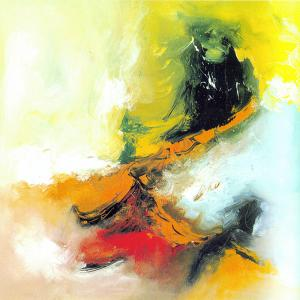
\includegraphics[width=\textwidth]{fig-i-am-abstract.jpg}
      \caption{我很抽象}
      \label{fig:i-am-abstract}
    \end{figure}
  \end{columns}
\end{frame}

\begin{frame}[fragile] % [fragile]参数使得能够插入代码
  \frametitle{定义抽象类}

  \begin{block}{}
    \begin{itemize}
    \item 在定义Java方法时可以只给出方法头,而不必给出方法的实现细节,这
      样的方法被称为{\Red 抽象方法}。
    \item 抽象方法必须用关键字{\Red abstract}修饰。
    \item 包含抽象方法的类必须声明为抽象类,用关键字{\Red abstract}修
      饰。
    \end{itemize}
  \end{block}


  \samp{抽象类示例}
  
  \begin{javaCode}
    public abstract class Animal { //定义为抽象类
      private int age;
      
      public void setAge(int age) {
        this.age = age;
      }
      
      public int getAge(){
        return age;
      }
      
      public abstract void eat(); //抽象方法
    }
  \end{javaCode}
\end{frame}

\begin{frame}[fragile] % [fragile]参数使得能够插入代码
  \frametitle{定义抽象类}

  \samp{抽象类继承}
  
  \begin{javaCode}
    public class Person extends Animal {
      private String name;
      public void setName(String name) {
        this.name = name;
      }
      public String getName() {
        return name;
      }
      public void eat() { //重写方法
        System.out.println("洗手→烹饪→摆餐具→吃喝→收摊儿");
      }
    }
  \end{javaCode}

  \begin{javaCode}
    public class Bird extends Animal {
      public void fly(){
        System.out.println("我心飞翔!");
      }
      public void eat(){  //重写方法
        System.out.println("直接吞食!");
      }
    }
  \end{javaCode}
\end{frame}

\begin{frame}[fragile] % [fragile]参数使得能够插入代码
  \frametitle{抽象类的特性与作用}

  \tta{抽象类的特性}

  \begin{itemize}[<+-| alert@+>]
  \item 子类必须实现其父类中的所有抽象方法,否则该子类也只能声明为抽象类。
  \item 抽象类不能被实例化。\pause\notice{问题} 抽象类能否有构造方法?
  \end{itemize}
  
  \pause
  
  \tta{抽象类的作用}
  
  抽象类主要是通过继承由其子类发挥作用,包括两方面:
  
  \begin{description}
  \item[\fbox{代码重用}] 子类可以重用抽象类中的属性和非抽象方法。
  \item[\fbox{规划}] 子类中通过抽象方法的重写来实现父类规划的功能。
  \end{description}
\end{frame}


\begin{frame}[fragile] % [fragile]参数使得能够插入代码
  \frametitle{抽象类的其他特性}
  
  \begin{itemize}[<+-| alert@+>]
  \item 抽象类中可以不包含抽象方法。{\kai 主要用于当一个类已经定义了多
      个更适用的子类时,为避免误用功能相对较弱的父类对象,干脆限制其实
      例化。}
  \item 子类中可以不全部实现抽象父类中的抽象方法,但此时子类也只能声明为抽象类。
  \item 父类不是抽象类,但在子类中可以添加抽象方法,此情况下子类必须声明为抽象类。
  \item 多态性对于抽象类仍然适用,可以将引用类型变量(或方法的形参)声明为抽象类的类型。
  \item 抽象类中可以声明static属性和方法,只要访问控制权限允许,这些属性和方法可以通
    过{\kai <类名>.<类成员>}的方法进行访问。
  \end{itemize}
\end{frame}

\section{接口}

\begin{frame}[fragile] % [fragile]参数使得能够插入代码
  \frametitle{接口(interface)}

  \begin{block}{接口}
    在科技辞典中,“接口”被解释为“两个不同系统(或子程序)交接并通过它
    彼此作用的部分。”
  \end{block}

  \pause

  在Java语言中,通过接口可以了解对象的交互界面,即明确对象提供的功能及
  其调用格式,而不需要了解其实现细节。

  \pause

  接口是抽象方法和常量值的定义的集合。从本质上讲,接口是一种特殊的{\Red 抽象
  类},这种抽象类中{\kai\Red 只包含常量定义和方法声明,而没有变量和方法的实现}。
\end{frame}

\begin{frame}[fragile] % [fragile]参数使得能够插入代码
\frametitle{定义接口}

接口中定义的属性必须是public static final的,而接口中定义的方法则必须
是public abstract的,因此这些关键字可以部分或全部省略。

\samp{接口示例(未简化)}

\begin{javaCode}
  public interface Runner {
    public static final int id = 1;
    public abstract void start();
    public abstract void run();
    public abstract void stop();
  }
\end{javaCode}

\samp{与上述代码等价的标准定义}

\begin{javaCode}
  public interface Runner {
    int id = 1;
    void start();
    void run();
    void stop();
  }
\end{javaCode}
\end{frame}

\begin{frame}[fragile] % [fragile]参数使得能够插入代码
  \frametitle{接口的实现}

  和继承关系类似,类可以{\Red\hei 实现}接口,且接口和实现类之间也存在多态性。

  \tta{类继承和接口实现的语法格式}

  \begin{javaCode}
    [<modifier>] class <name> [extends <superclass>] [implements <interface> [,<interface>]* ] {
      <declarations>*
    }
  \end{javaCode}
\end{frame}

\begin{frame}[fragile] % [fragile]参数使得能够插入代码
  \frametitle{接口的实现}

  \samp{接口实现示例}

  \begin{javaCode}
    public class Person implements Runner {
      public void start() {
        System.out.println("弯腰、蹬腿、咬牙、瞪眼、开跑");
      }
      public void run(){
        System.out.println("摆动手臂、维持直线方向");
      }
      public void stop(){
        System.out.println("减速直至停止、喝水");
      }
    }
  \end{javaCode}
\end{frame}

\begin{frame}[fragile] % [fragile]参数使得能够插入代码
  \frametitle{接口的实现}

  通过接口可以指明多个类需要实现的方法,而这些类还可以根据需要继承各自
  的父类。或者说,{\Red\kai 通过接口可以实现不相关类的相同行为,而不需要考
    虑这些类之间的层次关系。}
  
  \begin{figure}
    \centering
    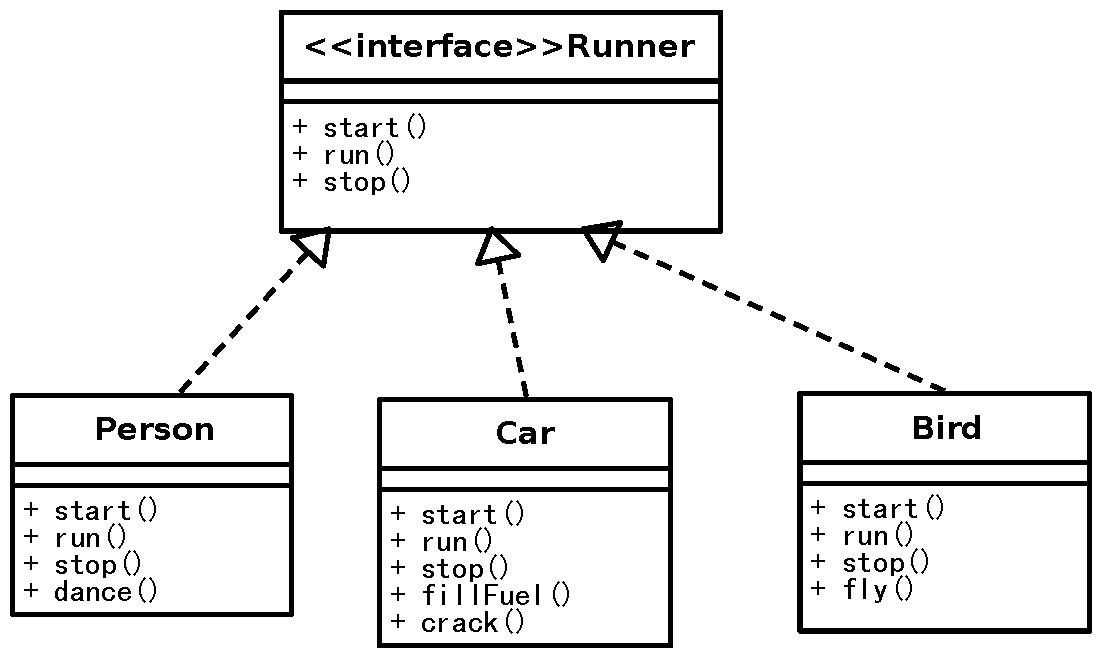
\includegraphics[width=0.5\textwidth]{fig-interface-implement-sample.pdf}
  \end{figure}

  \notice{类允许实现多重接口}

  \codeset{package sample.advance.interfacesample}

\end{frame}


\begin{frame}[fragile] % [fragile]参数使得能够插入代码
\frametitle{接口间的继承}

与接口的多重实现情况类似,由于不担心方法追溯调用上的不确定性,接口之间
的继承允许“多重继承”的情况。

\begin{javaCode}
interface A {
  public void ma();
}
interface B {
  public int mb(int i);
}
interface C extends A,B {  //接口的多重继承
  public String mc();
}
class D implements C {
  public void ma() {
    System.out.println("Implements method ma()!");
  }
  public int mb(int i) {
    return 2000 + i;
  }
  public String mc() {
    return "Hello!";
  }
}
\end{javaCode}
{\footnotesize \Mage 上述代码中的D类缺省继承了Object类,直接实现了接口C,间接实现了接口A和B,由于多态性的机
制,将来D类的对象可以当作Object、C、A或B等类型使用。}
\end{frame}

\begin{frame}[fragile] % [fragile]参数使得能够插入代码
  \frametitle{接口特性总结}

  \begin{itemize}[<+-| alert@+>]
  \item 通过接口可以实现不相关类的相同行为,而不需要考虑这些类之间的层次关系。
  \item 接口可以被多重实现。
  \item 接口可以继承其它的接口,并添加新的属性和抽象方法,接口间支持多重继承。
  \end{itemize}
\end{frame}
%%%%%%%%%%%%%%%%%%%%%%%%%%%%%%%%%%%%%%%%%%%%%%%%
\section{抽象类和接口剖析}

\begin{frame}[fragile]
  \frametitle{语法层面的区别}

  \begin{alertblock}{}
    \hei\centering 概念差异 —— 语法差异 —— 用法差异 —— 设计哲学
  \end{alertblock}

  \pause
  
  \begin{itemize}[<+-| alert@+>]
  \item 抽象类可以提供成员方法的实现细节,而接口中只能存在public
    abstract方法
  \item 抽象类中的成员变量可以为各种类型,而接口中的成员变量只能
    是public static final类型
  \item 抽象类可以有静态代码块和静态方法,接口中不能含有静态代码块以及
    静态方法
  \item 一个类只能继承一个抽象类,而一个类却可以实现多个接口
  \end{itemize}
\end{frame}

\begin{frame}[fragile]
  \frametitle{设计层面的区别}

  \begin{block}{}
    \begin{itemize}\kai
    \item 抽象类是对类的抽象(可以抽象但不宜实例化),而接口是对行为的
      抽象。
    \item 抽象类是对类整体进行抽象,包括属性、行为,但是接口却是对类局
      部(行为)进行抽象。
    \end{itemize}
  \end{block}

  \pause

  \begin{block}{}
    \begin{itemize}\kai
    \item 抽象类作为很多子类的父类,它是一种模板式设计。{\Red 模板式设计:模
      板代表公共部分,公共部分需要改的则改动模板即可。}
    \item 而接口是一种行为规范,它是一种辐射式设计。{\Red 辐射式设计:接口
      进行了变更,则所有实现类都必须进行相应的改动。}
    \end{itemize}
  \end{block}  

\end{frame}

\begin{frame}[fragile]
  \frametitle{怎样才是合理的设计?(门和警报的示例)}

  一般来说,门都有\fbox{open()}和\fbox{close()}这两个动作。通过抽象类和
  接口来定义这个抽象概念:

  \begin{columns}
    \column{0.5\textwidth}

    \begin{javaCode}
      abstract class Door {
        public abstract void open();
        public abstract void close();
      }
    \end{javaCode}
    \column{0.5\textwidth}

    \begin{javaCode}
      interface Door {
        public abstract void open();
        public abstract void close();
      }
    \end{javaCode}
  \end{columns}

  \pause
  
  \notice{问题} 如果现在我们需要门具有报警\fbox{alarm()}的功能该如何实
  现?
\end{frame}

\begin{frame}[fragile]
  \frametitle{怎样才是合理的设计?(门和警报的示例)}

  \tta{思路一} 
  
  将这三个功能都放在抽象类里面,这样一来所有继承这个抽象类的子类都具备
  了报警功能,但是有的门并不一定需要具备报警功能。\pause {\hei\Red 不合理抽象}

  \pause
  
  \tta{思路二} 

  将这三个功能都放在接口里面,但需要用到报警功能的类就需要实现这个接口
  中的open()和close(),也许这个类根本就不具备open()和close()这两个功能,
  比如火灾报警器。\pause {\hei\Red 不合理规划}

\end{frame}

\begin{frame}[fragile]
  \frametitle{怎样才是合理的设计?(门和警报的示例)}

  Door的open() 、close()和alarm()根本就属于两个不同范畴内的行为:

  \begin{itemize}
  \item open()和close()属于门本身固有的行为特性。
  \item alarm()属于延伸的附加行为。
  \end{itemize}

  \pause
  
  \tta{更为合理的思路} 

  \ding{182} 单独将报警设计为一个接口,包含alarm()行为;\ding{183} Door设计为单独
  的抽象类,包含open()和close()两种行为;\ding{184} 设计一个报警门继
  承Door类和实现Alarm接口。

  \codeset{package sample.advance.door}
\end{frame}



%% 1)抽象类是对一种事物的抽象,即对类抽象,而接口是对行为的抽象。抽象类是对整个类整体进行抽象,包括属性、行为,但是接口却是对类局部(行为)进行抽象。举个简单的例子,飞机和鸟是不同类的事物,但是它们都有一个共性,就是都会飞。那么在设计的时候,可以将飞机设计为一个类Airplane,将鸟设计为一个类Bird,但是不能将 飞行 这个特性也设计为类,因此它只是一个行为特性,并不是对一类事物的抽象描述。此时可以将 飞行 设计为一个接口Fly,包含方法fly(),然后Airplane和Bird分别根据自己的需要实现Fly这个接口。然后至于有不同种类的飞机,比如战斗机、民用飞机等直接继承Airplane即可,对于鸟也是类似的,不同种类的鸟直接继承Bird类即可。从这里可以看出,继承是一个 "是不是"的关系,而 接口 实现则是 "有没有"的关系。如果一个类继承了某个抽象类,则子类必定是抽象类的种类,而接口实现则是有没有、具备不具备的关系,比如鸟是否能飞(或者是否具备飞行这个特点),能飞行则可以实现这个接口,不能飞行就不实现这个接口。
%%
%% 2)设计层面不同,抽象类作为很多子类的父类,它是一种模板式设计。而接口是一种行为规范,它是一种辐射式设计。什么是模板式设计?最简单例子,大家都用过ppt里面的模板,如果用模板A设计了ppt B和ppt C,ppt B和ppt C公共的部分就是模板A了,如果它们的公共部分需要改动,则只需要改动模板A就可以了,不需要重新对ppt B和ppt C进行改动。而辐射式设计,比如某个电梯都装了某种报警器,一旦要更新报警器,就必须全部更新。也就是说对于抽象类,如果需要添加新的方法,可以直接在抽象类中添加具体的实现,子类可以不进行变更;而对于接口则不行,如果接口进行了变更,则所有实现这个接口的类都必须进行相应的改动。
%%
%% 下面看一个网上流传最广泛的例子:门和警报的例子:门都有open( )和close( )两个动作,此时我们可以定义通过抽象类和接口来定义这个抽象概念:
%%
%%
%%abstract class Door {
%%    public abstract void open();
%%    public abstract void close();
%%}
%%  或者:
%%
%%interface Door {
%%    public abstract void open();
%%    public abstract void close();
%%}
%%  但是现在如果我们需要门具有报警alarm( )的功能,那么该如何实现?下面提供两种思路:
%%


%%%%%%%%%%%%%%%%%%%%%%%%%%%%%%%%%%%%%%%%%%%%%%%%
\section{嵌套类}
\begin{frame}[fragile] % [fragile]参数使得能够插入代码
  \frametitle{什么是嵌套类}

  Java语言支持类的嵌套定义,即允许将一个类定义在其他类的内部,其中内层的类被称为嵌套类。

  \tta{嵌套类的分类}
  
  \begin{description}
  \item[\fbox{静态嵌套类(Static Nested Class)}] 使用static修饰的嵌套类
  \item[\fbox{内部类(Inner Class)}] 非static的嵌套类
    \begin{description}
    \item[普通内部类] 在类中的方法或语句块外部定义的非static类。
    \item[局部内部类] 定义在方法或语句块中的类,也称局部类。
    \item[匿名内部类] 定义在方法或语句块中,该类没有名字、只能在其所在
      之处使用一次。
    \end{description}
  \end{description}

  {\kai (仅讲授包含静态嵌套类和匿名内部类,其他自行学习)}
  
\end{frame}


\begin{frame}[fragile] % [fragile]参数使得能够插入代码
  \frametitle{静态嵌套类}

  \tta{静态嵌套类的特征}
  
  \begin{itemize}
  \item {\hei 静态嵌套类不再依赖/引用外层类的特定对象,只是隐藏在另一个
      类中而已。}
  \item 由于静态嵌套类的对象不依赖外层类的对象而独立存在,因而可以直接
    创建,进而也就无法在静态嵌套类中直接使用其外层类的非static成员。
  \end{itemize}

  \codeset{sample.advance.nestedclass.StaticNestedClassSample.java}
\end{frame}

%%\begin{frame}[fragile] % [fragile]参数使得能够插入代码
%%\frametitle{使用内部类\ding{182}}
%%
%%\samp{JavaSE\_03/TestInnerClass.java}
%%
%%\samp{TestInner.java}
%%\begin{javaCode}
%%class A {
%%  private int s;
%%  public class B {
%%    public void mb() {
%%      s = 100;
%%      System.out.println("在内部类 B 中 s=" + s);
%%    }
%%  }
%%  public void ma() {
%%    B i = new B();
%%    i.mb();
%%  }
%%}
%%
%%public class TestInner {
%%  public static void main(String args[]) {
%%    A o = new A();
%%    o.ma();
%%  }
%%}
%%\end{javaCode}
%%
%%{\small \Mage 上述程序编译后生成三个文件:TestInner.class, A.class, A\$B.class。}
%%\end{frame}
%%
%%\begin{frame}[fragile] % [fragile]参数使得能够插入代码
%%\frametitle{使用内部类\ding{182}}
%%
%%\wxd{TestInner.java运行时的内存状态}
%%
%%系统创建一个外层类的对象o,并将其实例变量s缺省初始化为0。
%%
%%\begin{figure}
%%\centering
%%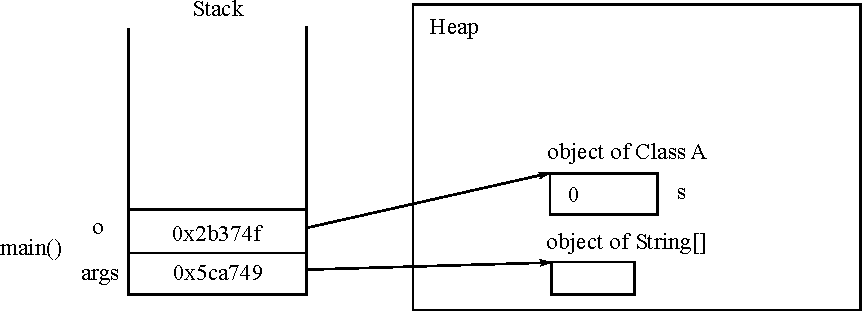
\includegraphics[width=0.8\textwidth]{innerclass01.pdf}
%%\end{figure}
%%
%%\end{frame}
%%
%%\begin{frame}[fragile] % [fragile]参数使得能够插入代码
%%\frametitle{使用内部类\ding{182}}
%%
%%\wxd{TestInner.java运行时的内存状态}
%%
%%调用对象o的成员方法ma(),首先为引用变量this分配空间以记录该方法本次运行时的当前对象,然后执行方法体中的第一条语句创建一个内部类B的对象i。
%%
%%\begin{figure}
%%\centering
%%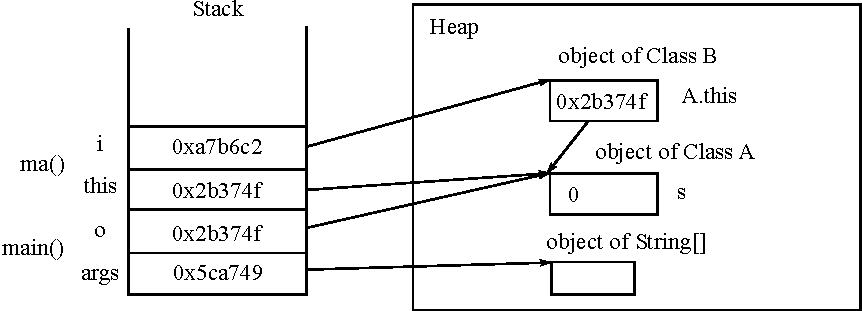
\includegraphics[width=0.8\textwidth]{innerclass02.pdf}
%%\end{figure}
%%
%%{\kai\small 此时,内部类B中虽然未显式的定义任何属性,但其对象i一经创建,即拥有一个系统自动添加的属性(实例变量),该属性的数据类型为外层类对象的句柄,该属性为只读,且可以使用约定标记<外层类名>.this访问。}
%%
%%\end{frame}
%%
%%\begin{frame}[fragile] % [fragile]参数使得能够插入代码
%%\frametitle{使用内部类\ding{182}}
%%
%%\wxd{TestInner.java运行时的内存状态}
%%
%%内部类对象i调用其成员方法mb()。
%%
%%\begin{figure}
%%\centering
%%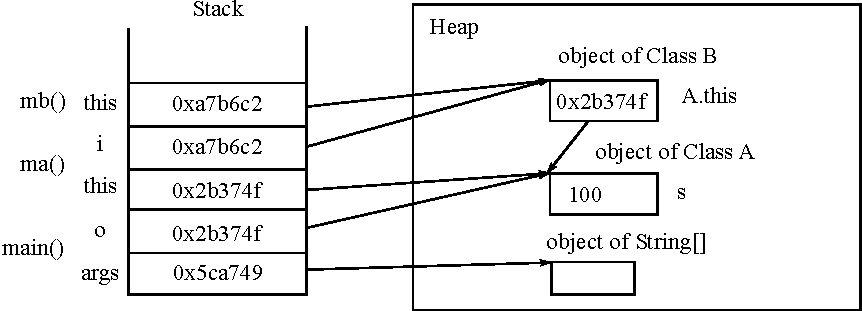
\includegraphics[width=0.8\textwidth]{innerclass03.pdf}
%%\end{figure}
%%
%%{\kai\small 在方法体中遇到变量s时,按照如下处理过程:首先在当前方法mb()中检索是否存在局部变量(包括方法形参)s,没有则继续查找方法的当前对象(内部类B中)是否存在成员变量s,没有则通过属性A.this检索当前对象所依赖的外层类对象,最终找到并操作该变量s并赋值为100。}
%%\end{frame}
%%
%%\begin{frame}[fragile] % [fragile]参数使得能够插入代码
%%\frametitle{使用内部类\ding{183}}
%%
%%在外部使用其他类中的内部类虽然不提倡,但也是允许的。此时,应指明其完整层次,并显式建立对
%%象间的依赖关系。
%%
%%\samp{A.java}
%%\begin{javaCode}
%%public class A {
%%  private int s;
%%  public class B {
%%    public void mb() {
%%      System.out.println(s);
%%    }
%%  }
%%}
%%\end{javaCode}
%%\samp{TestInner2.java}
%%\begin{javaCode}
%%public class TestInner2 {
%%  public static void main(String[] args) {
%%    A a = new A();
%%    // 创建一个依赖于 a 而存在的 b
%%    A.B b = a.new B();
%%    b.mb();
%%  }
%%}
%%\end{javaCode}
%%\end{frame}
%%
%%\begin{frame}[fragile] % [fragile]参数使得能够插入代码
%%\frametitle{使用内部类\ding{184}}
%%
%%内部类中出现变量命名冲突时,可以使用内部类对象的特殊属性“<外层类名>.this”来访问其所依赖
%%外层类对象的成员。
%%\samp{TestInner3.class}
%%\begin{javaCode}
%%class A {
%%  private int s = 111;
%%  public class B {
%%    private int s = 222;
%%    public void mb(int s) {
%%      System.out.println(s);  // 局部变量 s
%%      System.out.println(this.s);  // 内部类对象的属性 s
%%      System.out.println(A.this.s); // 外层类对象属性 s
%%    }
%%  }
%%}
%%
%%public class TestInner3 {
%%  public static void main(String args[]) {
%%    A a = new A();
%%    A.B b = a.new B();
%%    b.mb(333);
%%  }
%%}
%%\end{javaCode}
%%{\small\Mage 输出结果为:333\textbackslash n 222\textbackslash n 111}
%%\end{frame}
%%
%%\begin{frame}[fragile] % [fragile]参数使得能够插入代码
%%\frametitle{局部内部类}
%%
%%局部内部类是定义在Java方法或语句块中的类型,相当于方法中的局部变量,其作用域仅限于其所在的方法体或者语句块。
%%
%%\begin{itemize}\kai
%%\item 局部类声明时不允许加public、private等访问控制修饰符。
%%\item 局部类也不允许定义static属性和方法,{\Red 除非局部类为静态类(后续讲述)}。
%%\item 局部类中不但可以访问其所在外层类的成员,还可以访问其所在方法/语句块中的局部变量,但
%%  这些变量必须声明为{\Red final}。
%%\end{itemize}
%%
%%\samp{JavaSE\_03/TestLocalInnerClass.java}
%%
%%{\hei\Red 不建议使用局部类。}
%%\end{frame}

\begin{frame}[fragile] % [fragile]参数使得能够插入代码
\frametitle{匿名内部类}

匿名内部类是局部类的一种简化。

{\kai 当我们只在一处使用到某个类型时,可以将之定义为局部类,进而如果我
  们只是创建并使用该类的一个实例的话,那么连类的名字都可以省略。}
\end{frame}

\begin{frame}[fragile] % [fragile]参数使得能够插入代码
  \frametitle{使用匿名内部类}

  \samp{Person.java}

  \begin{javaCode}
    public abstract class Person {
      private String name;
      private int age;
      
      public Person() {}
      
      public Person(String name, int age) {
        this.name = name;
        this.age = age;
      }
      
      public String getInfo() {
        return "Name: " + name + "\t Age: " + age;
      }
      
      public abstract void work();
    }  
  \end{javaCode}
\end{frame}

\begin{frame}[fragile] % [fragile]参数使得能够插入代码
  \frametitle{使用匿名内部类}

  \samp{TestAnonymous.java}

  \begin{javaCode}
    public class TestAnonymous {
      public static void main(String[] args) {
        Person sp = new Person() { // 匿名内部类
          public void work() {
            System.out.println("个人信息:" + this.getInfo());
            System.out.println("I am sailing.");
          }
        };
        
        sp.work();
      }
    }
  \end{javaCode}

  \pause
  
  \ttc{上述代码的解释}

  {\small\Red 定义一个新的Java内部类,该类本身没有名字,但继承了指定的父
    类Person,并在此匿名子类中重写了父类的work()方法,然后立即创建了一
    个该匿名子类的对象,再将其地址保存到引用变量sp中待用。}
\end{frame}

\begin{frame}[fragile] % [fragile]参数使得能够插入代码
  \frametitle{使用匿名内部类}

  由于匿名类没有类名,而构造方法必须与类同名,所以{\hei 匿名类不能显式的定义构造方
    法},但系统允许在创建匿名类对象时将参数传给父类构造方法(使用父类的构造方法)。

  \begin{javaCode}
    Person sp = new Person("Kevin", 30) {
      public void work() {
        System.out.println("个人信息:" + this.getInfo());
        System.out.println("I am sailing.");
      }
    };
  \end{javaCode}
\end{frame}

\begin{frame}[fragile] % [fragile]参数使得能够插入代码
  \frametitle{使用匿名内部类}

  匿名类除了可以继承现有父类之外,还可以实现接口,但不允许实现多个接口,
  且实现接口时就不能再继承父类了,反之亦然。

  \samp{Swimmer.java}

  \begin{javaCode}
    public interface Swimmer {
      public abstract void swim();
    }
  \end{javaCode}

  \samp{TestAnonymous2.java}
  
  \begin{javaCode}
    public class TestAnonymous2 {
      public static void main(String[] args) {
        TestAnonymous2 ta = new TestAnonymous2();
        ta.test(new Swimmer() { // 匿名类实现接口
          public void swim() {
            System.out.println("I am swimming.");
          }
        });
        
        public void test(Swimmer swimmer) {
          swimmer.swim();
        }
      }
    }
  \end{javaCode}
\end{frame}

\section{枚举类型}
\begin{frame}[fragile] % [fragile]参数使得能够插入代码
\frametitle{什么是枚举类型}

Java SE 5.0开始,引入了一种新的引用数据结构{\hei\Red 枚举类
  型}。{\kai 枚举类型均自动继承java.lang.Enum类,使用一组常量值来表示
  特定的数据集合,该集合中数据的数目确定(通常较少),且这些数据只能
  取预先定义的值。}

\begin{javaCode}
  public enum Week {
    MON, TUE, WED, THU, FRI, SAT, SUN
  }
\end{javaCode}

\notice{无枚举类型前如何解决上述需求?}

一般采用声明多个整型常量的做法实现枚举类的功能。

\begin{javaCode}
  public class Week {
    public static final int MON = 1;
    public static final int TUE = 2;
    ...
  }    
\end{javaCode}
\end{frame}

%%\begin{frame}[fragile] % [fragile]参数使得能够插入代码
%%\frametitle{使用枚举类型}
%%\begin{javaCode}
%%public enum Week {
%%  MON, TUE, WED, THU, FRI, SAT, SUN
%%}  
%%\end{javaCode}
%%\begin{javaCode}
%%public class TestEnum {
%%  public static void main(String[] args) {
%%    TestEnum te = new TestEnum();
%%    te.work(Week.SUN);
%%  }
%%  public void work(Week day) {
%%    if (day.equals(Week.SAT)) {
%%      System.out.println("购物!");
%%    }else if (day.equals(Week.SUN)) {
%%      System.out.println("祈祷!");
%%    } else {
%%      System.out.println("工作!");
%%    }
%%  }
%%}
%%\end{javaCode}
%%\end{frame}

%%\begin{frame}[fragile] % [fragile]参数使得能够插入代码
%%\frametitle{遍历枚举类型常量值}
%%
%%可以使用静态方法values()遍历枚举类型常量值。
%%
%%\samp{ListEnum.java}
%%\begin{javaCode}
%%public class ListEnum {
%%  public static void main(String[] args) {
%%    Week[] days = Week.values();
%%    for(Week d: days) {
%%      System.out.println(d);
%%    }
%%  }
%%}
%%\end{javaCode}
%%\end{frame}

\begin{frame}[fragile] % [fragile]参数使得能够插入代码
\frametitle{组合使用枚举类型与switch}

\codeset{package sample.advance.enumclass}

\pause

\notice{注意}

\begin{enumerate}
\item case字句必须省略其枚举类型的前缀,即只需要写成 case SUN:,而不允许写成 case
  Week.SUN:,否则编译出错。
\item 不必担心系统无法搞清这些常量名称的出处,因为switch后的小括号中的表达式已经指明本次
  要区分处理的是Week类型常量。
\end{enumerate}
\end{frame}

\begin{frame}[fragile]
  \frametitle{本节习题}

  \wxd{简答题}
  \begin{enumerate}
  \item 分析抽象类和接口的异同,说明抽象类和接口的作用。
  \end{enumerate}

  \wxd{小编程}
  \begin{enumerate}
  \item 为Eclipse安装Amateras插件
    (https://takezoe.github.io/amateras-update-site/),并尝试使用该插
    件为示例代码或自己编写的代码自动生成类图。
  \end{enumerate}

\end{frame}



% TKS %%%%%%%%%%%%%%%%%%%%%%%%%%%%%%%%%%%%%%%%%%%%%%
\begin{frame}[focus]
\centering
{\Huge {THE END}} \\
\vspace{5mm}
{\Large wangxiaodong@ouc.edu.cn} \\
\end{frame}
%%%%%%%%%%%%%%%%%%%%%%%%%%%%%%%%%%%%%%%%%%%%%%%%%%%%
\end{document}

%%%%%%%%%%%%%%%%%%%%%%%%%%%%%%%%%%%%%%%%%%%%%%%%%%%%%%%%%%%%%%%%%%%%%%%%%%%%%%%
% Full instructions available at:
% https://github.com/elauksap/focus-beamertheme

\documentclass{beamer}
\usetheme{focus}

% package for font
\usepackage{fontspec}
\defaultfontfeatures{Mapping=tex-text}  %%如果没有它,会有一些 tex 特殊字符无法正常使用,比如连字符。
\usepackage{xunicode,xltxtra}
\usepackage[BoldFont,SlantFont,CJKnumber,CJKchecksingle]{xeCJK}  % \CJKnumber{12345}: 一万二千三百四十五
\usepackage{CJKfntef}  %%实现对汉字加点、下划线等。
\usepackage{pifont}  % \ding{}
% package for math
\usepackage{amsfonts}
% package for graphics
\usepackage[americaninductors,europeanresistors]{circuitikz}
\usepackage{tikz}
\usetikzlibrary{plotmarks}  % placements=positioning
\usepackage{graphicx}  % \includegraphics[]{}
\usepackage{subfigure}  %%图形或表格并排排列
% package for table
\usepackage{colortbl,dcolumn}  %% 彩色表格
\usepackage{multirow}
\usepackage{multicol}
\usepackage{booktabs}
% package for code
\usepackage{fancyvrb}
\usepackage{listings}
% setting for font
%%\setCJKmainfont{Adobe Kaiti Std}
\setCJKmainfont{SimSun}
%%\setCJKmainfont{Microsoft YaHei}
%%\setCJKmainfont{FangSong_GB2312} 
%%\setmainfont{Times New Roman}
%\setsansfont[Mapping=tex-text]{Adobe Song Std}
%如果装了Adobe Acrobat,可在font.conf中配置Adobe字体的路径以使用其中文字体。
%也可直接使用系统中的中文字体如SimSun、SimHei、微软雅黑等。
%原来beamer用的字体是sans family;注意Mapping的大小写,不能写错。
%设置字体时也可以直接用字体名,以下三种方式等同:
%\setromanfont[BoldFont={黑体}]{宋体}
%\setromanfont[BoldFont={SimHei}]{SimSun}
%\setromanfont[BoldFont={"[simhei.ttf]"}]{"[simsun.ttc]"}

% font setting by xeCJK
\setCJKfamilyfont{NSimSun}{NSimSun}
\newcommand{\song}{\CJKfamily{NSimSun}}
%%%\setCJKfamilyfont{AdobeSongStd}{Adobe Song Std}
%%%\newcommand{\AdobeSong}{\CJKfamily{AdobeSongStd}}
\setCJKfamilyfont{FangSong}{FangSong_GB2312}
\newcommand{\fang}{\CJKfamily{FangSong}}
%%%\setCJKfamilyfont{AdobeFangsongStd}{Adobe Fangsong Std}
%%%\newcommand{\AdobeFang}{\CJKfamily{AdobeFangsongStd}}
\setCJKfamilyfont{SimHei}{SimHei}
\newcommand{\hei}{\CJKfamily{SimHei}}
%%%\setCJKfamilyfont{AdobeHeitiStd}{Adobe Heiti Std}
%%%\newcommand{\AdobeHei}{\CJKfamily{AdobeHeitiStd}}
\setCJKfamilyfont{KaiTi}{KaiTi_GB2312}
\newcommand{\kai}{\CJKfamily{KaiTi}}
%%%\setCJKfamilyfont{AdobeKaitiStd}{Adobe Kaiti Std}
\newcommand{\AdobeKai}{\CJKfamily{AdobeKaitiStd}}
\setCJKfamilyfont{LiSu}{LiSu}
\newcommand{\li}{\CJKfamily{LiSu}}
\setCJKfamilyfont{YouYuan}{YouYuan}
\newcommand{\you}{\CJKfamily{YouYuan}}
\setCJKfamilyfont{FZJingLei}{FZJingLeiS-R-GB}
\newcommand{\jinglei}{\CJKfamily{FZJingLei}}
\setCJKfamilyfont{MSYH}{Microsoft YaHei}
\newcommand{\msyh}{\CJKfamily{MSYH}}

\setbeamerfont{frametitle}{series=\Large\hei} % 修改Beamer标题字体

\graphicspath{{figures/}}  %%图片路径
\renewcommand\figurename{图}

% setting for pdf
\hypersetup{% pdfpagemode=FullScreen,%
  pdfauthor={Xiaodong Wang},%
  pdftitle={Title},%
  CJKbookmarks=true,%
  bookmarksnumbered=true,%
  bookmarksopen=false,%
  plainpages=false,%
  colorlinks=true,%
  citecolor=green,%
  filecolor=magenta,%
  linkcolor=blue,%red(default)
  urlcolor=cyan}

% setting for fontspec
\XeTeXlinebreaklocale "zh"  %%表示用中文的断行
\XeTeXlinebreakskip = 0pt plus 1pt minus 0.1pt  %%多一点调整的空间
%%%%%

% 自定义颜色
\def\Red{\color{red}}
\def\Green{\color{green}}
\def\Blue{\color{blue}}
\def\Mage{\color{magenta}}
\def\Cyan{\color{cyan}}
\def\Brown{\color{brown}}
\def\White{\color{white}}
\def\Black{\color{black}}

\lstnewenvironment{xmlCode}[1][]{% for Java
  \lstset{
    basicstyle=\tiny\ttfamily,%
    columns=flexible,%
    framexleftmargin=.7mm, %
    % frame=shadowbox,%
    % rulesepcolor=\color{cyan},%
     frame=single,%
    backgroundcolor=\color{white},%
    xleftmargin=4\fboxsep,%
    xrightmargin=4\fboxsep,%
    numbers=left,numberstyle=\tiny,%
    numberblanklines=false,numbersep=7pt,%
    language=xml, %
    }\lstset{#1}}{}

\lstnewenvironment{javaCode}[1][]{% for Java
  \lstset{
    basicstyle=\tiny\ttfamily,%
    columns=flexible,%
    framexleftmargin=.7mm, %
    frame=shadowbox,%
    rulesepcolor=\color{cyan},%
    % frame=single,%
    backgroundcolor=\color{white},%
    xleftmargin=4\fboxsep,%
    xrightmargin=4\fboxsep,%
    numbers=left,numberstyle=\tiny,%
    numberblanklines=false,numbersep=7pt,%
    language=Java, %
    }\lstset{#1}}{}

\lstnewenvironment{shCode}[1][]{% for Java
  \lstset{
    basicstyle=\scriptsize\ttfamily,%
    columns=flexible,%
    framexleftmargin=.7mm, %
    frame=shadowbox,%
    rulesepcolor=\color{brown},%
    % frame=single,%
    backgroundcolor=\color{white},%
    xleftmargin=4\fboxsep,%
    xrightmargin=4\fboxsep,%
    numbers=left,numberstyle=\tiny,%
    numberblanklines=false,numbersep=7pt,%
    language=sh, %
    }\lstset{#1}}{}

\newcommand\ask[1]{\vskip 4bp \tikz \node[rectangle,rounded corners,minimum size=6mm,
  fill=white,]{\Cyan \includegraphics[height=1.5cm]{question} \Large \msyh #1};}

\newcommand\wxd[1]{\vskip 4bp \tikz \node[rectangle,minimum size=6mm,
  fill=blue!60!white,]{\White \ding{118} \msyh #1};}

\newcommand\cxf[1]{\vskip 4bp \tikz \node[rectangle,rounded corners,minimum size=6mm,
  fill=purple!60!white,]{\White \ding{42} \msyh #1};}

\newcommand\xyy[1]{\vskip 2bp \tikz \node[rectangle,minimum size=3mm,
  fill=black!80!white,]{\White \msyh\scriptsize #1};}

\newcommand\tta[1]{\vskip 4bp \tikz \node[rectangle,minimum size=6mm,
  fill=blue!60!white,]{\White \ding{118} \msyh #1};}

\newcommand\ttb[1]{\vskip 4bp \tikz \node[rectangle,rounded corners,minimum size=6mm,
  fill=purple!60!white,]{\White \ding{42} \msyh #1};}

\newcommand\ttc[1]{\vskip 2bp \tikz \node[rectangle,minimum size=3mm,
  fill=black!80!white,]{\White \msyh\scriptsize #1};}

\newcommand\homework[1]{\vskip 2bp \tikz \node[rectangle,minimum size=3mm,
  fill=red!80!white,]{\White \ding{45} \msyh\scriptsize 课后小作业 } ; {\kai\small #1}} 

\newcommand\notice[1]{\vskip 4bp \tikz \node[rectangle,rounded corners,minimum size=6mm,
  fill=red!80!white,]{\White \scriptsize \ding{42} \msyh #1};}

\newcommand\samp[1]{\vskip 2bp \tikz \node[rectangle,minimum size=3mm,]{\Mage\msyh \small CODE \ding{231} \Black #1};\vskip -8bp}

\newcommand\codeset[1]{\vskip 2bp \tikz \node[rectangle,minimum
  size=3mm]{\Mage\msyh \small 课程配套代码 \ding{231} \Black
    #1};\vskip -4bp}

\newcommand\pptlink[2]{\vskip 4bp \tikz \node[rectangle,rounded corners,minimum size=6mm,
  fill=blue!70!white,]{\href{run:#1}{\White \scriptsize \msyh 动画演示 #2}};}


\makeatletter
\newcommand{\Extend}[5]{\ext@arrow 0099{\arrowfill@#1#2#3}{#4}{#5}}
\makeatother
%%%%%%%%%%%%%%%%%%%%%%%%%%%%%%%%%%%%%%%%%%%%%%%%%%%%%%%%%%%%%%%%%%%%%%%%%%%%%%%
\title{\hei JAVA应用与开发\\  泛\quad 型}
\subtitle{\it 让我们愉快的Coding起来吧...}
\author{王晓东}
\titlegraphic{\vspace{-8em}
\includegraphics[height=10cm]{static/ouc.pdf}\vspace{-6em}} 
\institute{中国海洋大学信息学院计算机系}
\date{\today}

\begin{document}

\begin{frame}
  \maketitle
\end{frame}

\begin{frame}
  \frametitle{学习目标}

  \begin{itemize}
  \item 理解泛型的概念,掌握其基本应用
    \begin{itemize}
    \item 集合框架中的泛型
    \item 泛型的向后兼容性
    \end{itemize}
  \item 掌握自定义泛型类和泛型方法
    \begin{itemize}
    \item 理解类型参数
    \item 理解差异性并能够定义自己的泛型类和泛型方法
    \item 受限制的类型参数
    \end{itemize}
  \item 学会处理泛型类型,包括使用通配符实现泛型容器遍历和操作
  \end{itemize}
\end{frame}

\begin{frame}
  \frametitle{大纲}
  \tableofcontents
\end{frame}

\section{泛型概念}

\begin{frame}[fragile] % [fragile]参数使得能够插入代码
  \frametitle{什么是泛型}

  \begin{block}{泛型(Generics)}
    泛型机制自JDK 5.0开始引入,其实质是{\hei\Blue 将原本确定不变的数据
      类型参数化}。

    作为对原有Java类型体系的扩充,使用泛型可以提高Java应用程序的类型安
    全、可维护性和可靠性。
  \end{block}
\end{frame}

\begin{frame}[fragile] 
  \frametitle{什么是泛型}

  \tta{集合框架中的数据造型问题}

  传统的集合容器为了提供广泛的适用性,会将所有加入其中的元素当
  作Object类型来处理。基于此原因,在实际使用时,我们必须将从集合中取出
  的元素值再强制转换(造型)为所期望的类型。

  \pause
  
  \notice{无泛型机制的集合容器}
  
  \begin{javaCode}
    Vector v = new Vector();
    v.addElement(new Person("Tom", 18));
    Person p = (Person) v.elementAt(0);
    p.showInfo();
  \end{javaCode}
  
\end{frame}

\begin{frame}[fragile]
  \frametitle{集合框架中的泛型}

  \begin{itemize}[<+-|alert@+>]
  \item 泛型允许编译器实施由开发者设定的附加类型约束,将类型检查
    从{\hei\Blue 运行时挪到编译时}进行,这样类型错误就可以在编译时暴露
    出来,而不是在运行时才发作(抛出ClassCastException运行异常)。
  \item 创建集合容器时规定其允许保存的元素类型,然后由编译器负责添加元
    素的类型合法性检查,在取用集合元素时则不必再进行造型处理。
  \end{itemize}
\end{frame}

\begin{frame}[fragile]
  \frametitle{集合框架中的泛型}

  \tta{在Vector中使用泛型}

  \codeset{sample.generics.VectorGenericsSample.java}
  
  \tta{在Hashtable中使用泛型}

  \codeset{sample.generics.HashtableGenericsSample.java}
  
\end{frame}

\begin{frame}[fragile] % [fragile]参数使得能够插入代码
  \frametitle{泛型的向后兼容性}

  \begin{block}{}
    \begin{itemize}
    \item Java语言中的泛型是维护向后兼容的,完全可以不采用泛型、而继续
      沿用过去的做法。
    \item 这些未加改造的旧式代码将无法使用泛型带来的便利和安全性。
    \end{itemize}
  \end{block}


  
  未启用泛型机制的代码在高版本编译器中会输出如下形式的编译提示信息:
  
  \begin{stdoutCode}
    注: VectorGenericsSample.java使用了未经检查或不安全的操作。
    注: 有关详细信息, 请使用 -Xlint:unchecked 重新编译。
  \end{stdoutCode}

  \pause
  
  可以使用SuppressWarnings注解关闭编译提示或警告信息:
  
  \begin{javaCode}
    @SuppressWarnings({"unchecked"})  
    public class VectorGenericsSample {
      ...
    }
  \end{javaCode}
\end{frame}




\section{泛型类与泛型方法}

\begin{frame}[fragile] % [fragile]参数使得能够插入代码
  \frametitle{类型参数}

  \begin{alertblock}{类型参数和泛型类}
    形如Vector<String>,其中,尖括号括起来的部分被称为{\Red\hei 类型参
      数},而这种由类型参数修饰的类型则被称为{\Blue\hei 泛型类}。
  \end{alertblock}

  \tta{注意}

  应在声明泛型类变量和创建对象时均给出类型参数,且两者应保持一致。
\end{frame}

\begin{frame}[fragile] % [fragile]参数使得能够插入代码
  \frametitle{类型参数}

  使用类型参数$E$进行泛型化处理的java.util.Vector类的定义代码摘要如下:
  
  \begin{javaCode}
    public class Vector<E> --- {
      public void addElement(E obj) { --- }
      public E elementAt(int index) { --- }
    }  
  \end{javaCode}

  \pause
  这里的$E$也称为“形式类型”参数。在实际使用该泛型类时,我们需要指定相应的
  具体类型,即实际类型参数。
  
  \begin{javaCode}
    Vector<String> v = new Vector<String>();  
  \end{javaCode}

  \pause
  编译器遇到Vector<String>类型变量时,即知道此Vector变量/对象的类型参
  数$E$已经被绑定为String类型,进而也就确定其addElement()方法的参数
  和elementAt()方法的返回值均为String类型。
\end{frame}




\begin{frame}[fragile] % [fragile]参数使得能够插入代码
  \frametitle{定义泛型类}

  \codeset{package sample.generics.userdefined}

  {\kai 代码示例中的泛型类PersonG可以在使用时通过类型参数T指定其属性secrecy的具体类型(以及该
    属性相应存/取方法的参数和返回值类型),进而提供了通用的信息存储能力。}

  \pause

  \tta{形式类型参数的编程惯例}

  \begin{table}
    \footnotesize
    \setlength{\extrarowheight}{1.2mm}
    \begin{tabular}{c|p{6cm}}
      {\bf 符号} & {\bf 意义}  \\
      K & 键,比如映射的键\\
      V & 值,比如List和Set的内容,或者Map中的值\\
      E & 元素,比如Vector<E>\\
      T & 泛型\\
    \end{tabular}
  \end{table}
\end{frame}

\begin{frame}[fragile] % [fragile]参数使得能够插入代码
  \frametitle{定义泛型类}

  \tta{使用受限制的类型参数}

  泛型机制允许开发者对类型参数进行附加约束。

  \begin{javaCode}
    import java.utils.Number;

    public class Point<T extends Number> {
      private T x;
      private T y;
      public Point() {}
      public Point(T x, T y) {
        this.x = x;
        this.y = y;
      }
      ...
    }
  \end{javaCode}

  \pause

  类型参数不能为基本数据类型,而java.lang.Number是所有数值型封装类(
  如Integer、Float、Double等)的父类型,于是限制泛型类Point的类型参数必
  须为Number或其子类类型,并使用extends关键字来标明这种继承层次上限制。
\end{frame}

\begin{frame}[fragile] % [fragile]参数使得能够插入代码
\frametitle{定义泛型方法}

与泛型类的情况类似,{\Red\hei 方法也可以被泛型化,且无论其所属的类是否为泛型类。}

\samp{泛型方法示例}

\begin{javaCode}
  public class Tool {
    public <T>T evaluate(T a, T b) {
      if(a.equals(b)) 
      return a;
      else
      return null;
    }
  }  
\end{javaCode}

\pause
\begin{itemize}
\item 上述代码中方法evaluate()声明中的“<T>”用于标明这是一个{\hei 泛型方
    法}。
\item 类型T是可变的,不必显示的告知编译器T具体取何值,但出现多处(两个
  形参、一个返回值类型)的这些值必须都相同。
\end{itemize}
\end{frame}

\begin{frame}[fragile] % [fragile]参数使得能够插入代码
\frametitle{定义泛型方法}

\tta{使用泛型方法,而不是定义泛型类的原则}

\begin{enumerate}[<+-|alert@+>]
\item 不涉及到类中的其他方法时,则应将之定义为泛型方法,因为泛型方法的
  类型参数是局部性的,这样可以简化其所在类型的声明和处理开销。
\item 要施加类型约束的方法为静态方法时,只能将之定义为泛型方法,因为静
  态方法不能使用其所在类的类型参数。
\end{enumerate}
\end{frame} 

\begin{frame}[fragile] % [fragile]参数使得能够插入代码
  \frametitle{对泛型的理解}
  
  \begin{itemize}
  \item 泛型类可以理解为具有广泛适用性、尚未最终定型的类型。
  \item Person<String>和Person<Double>属于同一个类,但确是不同的类型。
  \item 同一个泛型类与不同的类型参数复合而成的类型间并不存在继承关系,即使是类型参数间存在
    继承关系时也是如此。\\
    {\kai 如:Vector<String>不是Vector<Object>的子类。}
  \end{itemize}
\end{frame}

\section{处理泛型类型}

\begin{frame}[fragile] % [fragile]参数使得能够插入代码
  \frametitle{遍历泛型Vector集合}

  \tta{遍历Vector<String>类型集合}
  
  \begin{javaCode}
    public void overview(Vector<String> v) {
      for(String o: v) {
        String.out.println(o);
      }
    }
  \end{javaCode}

  \pause

  \notice{遍历其他类型参数的Vector集合元素该怎么办?}

  难道要定义overview(Vector<Person> v)、overview(Vector<Integer> v) ...
  
  显然过于繁琐,引用泛型机制后代码的通用性似乎不如从前?
\end{frame}

\begin{frame}[fragile] % [fragile]参数使得能够插入代码
  \frametitle{泛型类型的处理方法}

  \tta{可能的处理方法(不要使用)}

  将遍历方法的形参定义为不带任何类型参数的原型类型Vector,但这样会破坏已有的类型安全性。

  \begin{javaCode}
    public void overview(Vector v) {
      for(Object o: v) {
        String.out.println(o);
      }
    }
  \end{javaCode}

  \pause
  
  \tta{使用通配符}

  为了解决类似泛型遍历的问题,Java泛型机制中引入了通配符“?”。

  \begin{javaCode}
    public void overview(Vector<?> v) {
      for(Object o : v) {
        System.out.println(o);
      }
    }
  \end{javaCode}
\end{frame}

\begin{frame}[fragile] % [fragile]参数使得能够插入代码
\frametitle{类型通配符}
\wxd{使用类型通配符的好处}

\begin{enumerate}
\item Vector<?>是任何泛型Vector的父类型,因此可以将Vector<String>、Vector<Integer>、
  Vector<Object>等作为实参传给overview(Vector<?> v)方法处理;
\item Vector<?>类型的变量在调用方法时是受到限制的——凡是必须知道具体类型参数才能进行的操作
  均被禁止。
\end{enumerate}

\begin{javaCode}
Vector<String> vs = new Vector<String>();
vs.add("Tom");
Vector<?> v = vs;
v.add("Billy");  //非法,编译器不知道具体类型参数
Object e = v.elementAt(0); //合法,允许检索元素,此时读取的元素均当作 Object 类型处理
System.out.println(e);
\end{javaCode}
\end{frame}

\begin{frame}[fragile] % [fragile]参数使得能够插入代码
\frametitle{类型通配符}

上述限制不等同于将Vector<?>变为“只读”,在不需要编译器确定类型参数的情况下也是可以修改集
合内容的,例如:
\begin{javaCode}
Vector<String> vs = new Vector<String>();
vs.add("Tom");
vs.add("Billy");
Vector<?> v = vs;
v.remove(new Integer(200));  //形参为 Object 类型,运行不受影响
v.clear(); //不需要参数,运行不受影响
\end{javaCode}
\end{frame}


%%%%%%%%%%%%%%%%%%%%%%%%%%
%% \begin{frame}
%% \frametitle{本章习题}
%% \begin{enumerate}
%% \item a
%% \item b
%% \end{enumerate}
%% \end{frame}

%% \begin{figure}
%% \centering
%% 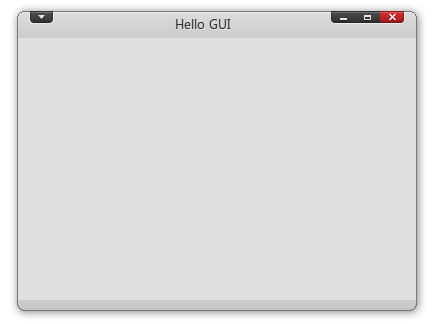
\includegraphics[width=0.6\textwidth]{fig01.png}
%% \end{figure}

% TKS %%%%%%%%%%%%%%%%%%%%%%%%%%%%%%%%%%%%%%%%%%%%%%
\begin{frame}[focus]
\centering
{\Huge {THE END}} \\
\vspace{5mm}
{\Large wangxiaodong@ouc.edu.cn} \\
\end{frame}
%%%%%%%%%%%%%%%%%%%%%%%%%%%%%%%%%%%%%%%%%%%%%%%%%%%%
\end{document}

% Week 05 %%
\chapter{控制台应用程序设计}
\label{chp:Terminal-application-programming}

\section*{基本信息}
\sline
\begin{description}
\item[课程名称:] Java应用与开发
\item[授课教师:] 王晓东
\item[授课时间:] 第五周
\item[参考教材:] 本课程参考教材及资料如下:
  \begin{itemize}
  \item 陈国君主编,Java程序设计基础(第5版),清华大学出版社,2015.5
  \item Bruce Eckel, Thinking in Java (3rd)
  \end{itemize}
\end{description}

\section*{教学目标}

\sline

\begin{enumerate}
\item 了解计算机人机交互发展
\item 掌握控制台程序设计开发中命令行参数、系统属性、标准输入输出的概
  念和相关Java操作
\item 掌握Java文件操作的的常用方法
\item 了解注解类型
\item 学会Jar归档工具,包括通过命令行或IDE进行Java程序归档的方法
\end{enumerate}

\section*{授课方式}

\sline
\begin{description}
\item[理论课:] 多媒体教学、程序演示
\item[实验课:] 上机编程
\end{description}

\newpage
\section*{教学内容}
\sline

\section{从古老的计算机谈起}

\subsection{冯诺依曼机}

我们的计算机是台遵守存储程序原理的冯诺依曼机器,基本组成包括{\hei 运算
  器、控制器(合起来是CPU)、存储器、输入设备、输出设备}。你所面对的一
切SOC也好,单板电脑也好,都是高度集成在一起的冯诺依曼机。

\subsubsection{1950年代的IBM 1401}

\begin{figure}[htb]
\centering
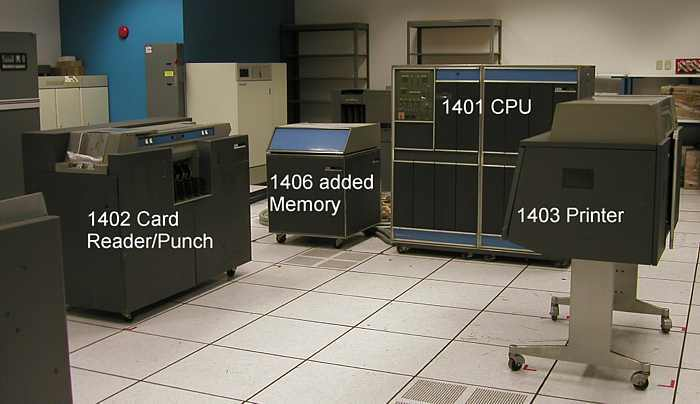
\includegraphics[width=0.6\textwidth]{images/Terminal-application-programming/fig-old-computer-01.jpg}
\caption{IBM 1401}
\label{fig:old-computer-01.jpg}
\end{figure}

\subsubsection{2010年代的树莓派开发板}

\begin{figure}[htb]
\centering
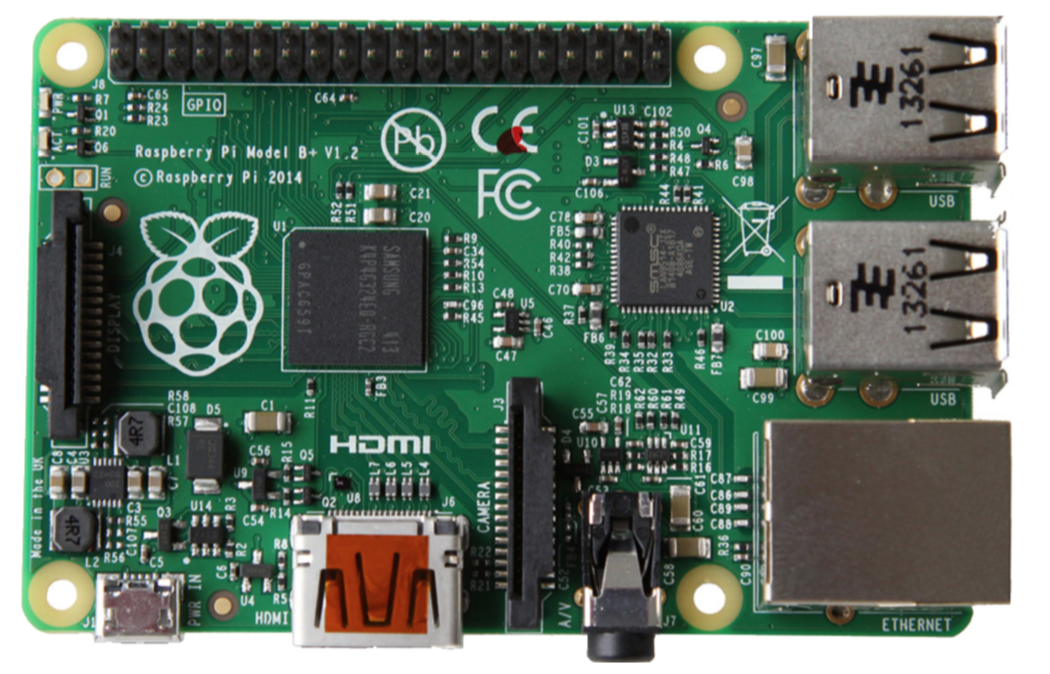
\includegraphics[width=0.5\textwidth]{images/Terminal-application-programming/fig-Raspberry-Pi-Board.png}
\caption{树莓派开发板}
\label{fig:Raspberry-Pi-Board}
\end{figure}


\subsection{人机交互}

\subsubsection{使用打孔卡片作为输入源,使用打印机作为输出设备}

一摞打孔卡片,就是一个“文件”。它可以是一段程序,也可以是一段程序需要使用的数据。

\begin{figure}[htb]
\centering
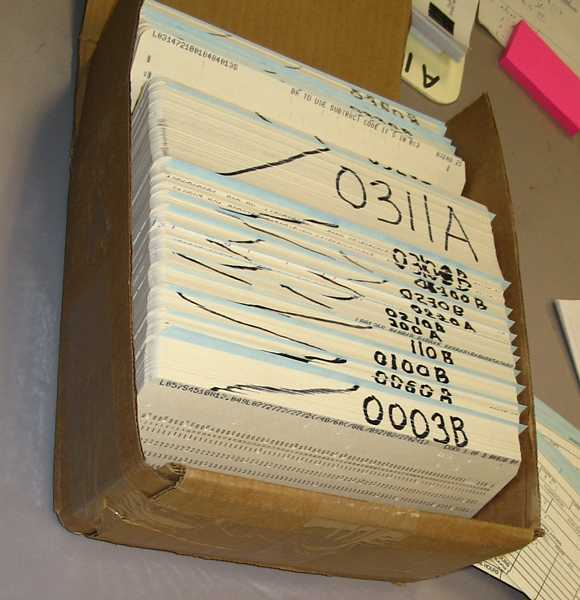
\includegraphics[width=0.5\textwidth]{images/Terminal-application-programming/fig-old-computer-input.jpg}
\caption{打孔卡片}
\label{fig:old-computer-input}
\end{figure}

\subsubsection{BASIC语言解释器}

纸带在70年代还很流行,当年比尔盖茨的BASIC语言解释器,就是存在纸带上的,现在已经成文物了。

\begin{figure}[htb]
\centering
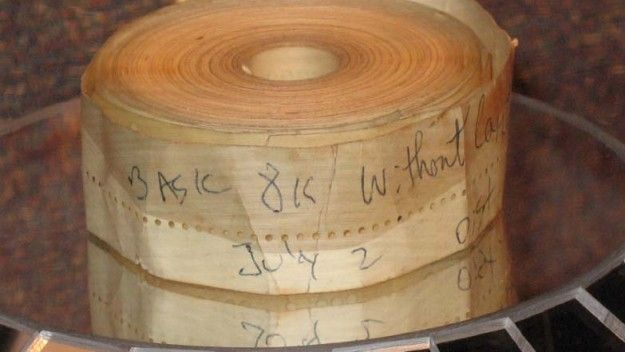
\includegraphics[width=0.6\textwidth]{images/Terminal-application-programming/fig-basic-lang-punch-tape.jpg}
\caption{打孔卡片}
\label{fig:basic-lang-punch-tape}
\end{figure}

\subsubsection{使用键盘作为输入设备,使用显示器作为输出设备}

\begin{figure}[htb]
  \begin{minipage}[t]{0.5\textwidth}
    \centering
    \fbox{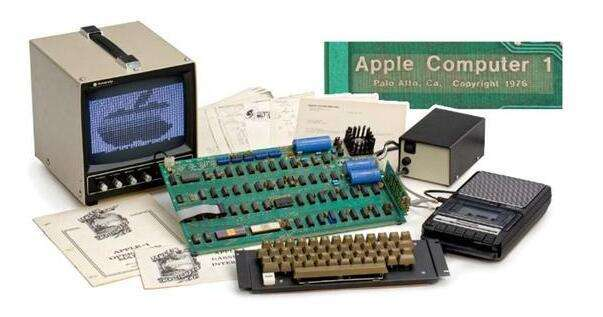
\includegraphics[width=.95\textwidth]{images/Terminal-application-programming/fig-apple-1-modules.jpg}}
    \caption{分立的Apple I}
    \label{fig:apple-1-modules}
  \end{minipage}
  \begin{minipage}[t]{0.5\textwidth}
    \centering
    \fbox{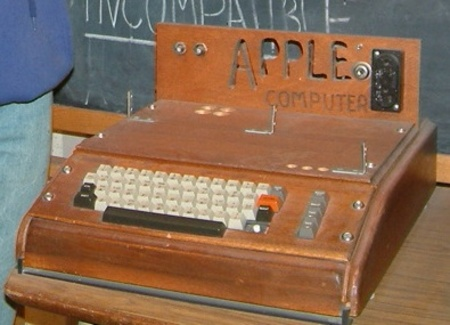
\includegraphics[width=.95\textwidth]{images/Terminal-application-programming/fig-apple-1.jpg}}
    \caption{Apple I}
    \label{fig:apple-1}
  \end{minipage}
\end{figure}

再厉害的科幻片导演,在飞船的人机交互界面表达上也未能超越同时代计算机的发展。

\begin{figure}[htb]
\centering
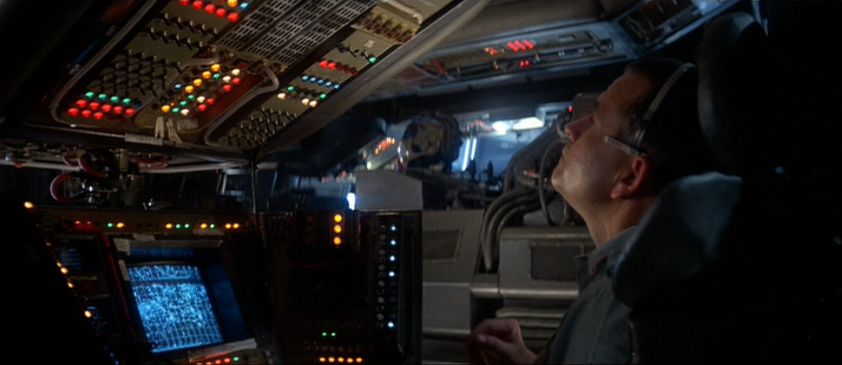
\includegraphics[width=\textwidth]{images/Terminal-application-programming/fig-Al012.png}
\caption{科幻定影中的计算机}
\label{fig:Al012}
\end{figure}

\section{命令行参数}

\subsection{命令行参数}

在启动时Java控制台应用程序,可以一次性地向程序中传递(零至多个)字符串参
数,这些参数被称为命令行参数。语法格式如下:

\begin{shCode}
  java <应用程序类名> [<命令行参数>]*
\end{shCode}

\notice{说明}

\begin{itemize}\kai
\item 命令行参数将被系统接收并静态初始化为一个一维的String数组对象,然后将之作为实参传给
  应用程序入口方法main()。
\item 命令行参数须使用空格符分隔,如果参数中包含空格符则必须使用双引号括起来。
\end{itemize}


\codeset{sample.commandline.CommandLineArgsSample.java}

Linux下运行程序方法如下:

\begin{shCode}
  > java CommandLineArgsSample Lisa "Billy" "Mr Brown"
\end{shCode}

Windows下运行程序方法如下:

\begin{shCode}
  C:\> java.exe CommandLineArgsSample Lisa "Billy" "Mr Brown" "a""b" 
\end{shCode}

输出结果为:

\begin{stdoutCode}
  Lisa
  Billy
  Mr Brown
\end{stdoutCode}


\subsection{可变参数方法}

\begin{itemize}
\item Java语言允许在定义方法时指定使用任意数量的参数,其格式是在参数
  类型后加“...”。
\item 可变长度参数必须放在参数列表的最后,一个方法最多只能包含一个可
  变长度参数。
\item 编译时,可变参数被当作{\Red\hei 一维数组处理}。
\end{itemize}

\begin{javaCode}
  public void myprint(String s, int i, Object... objs) { // 可变参数方法
    System.out.println(s.toUpperCase()); 
    System.out.println(100 * i);
    for(Object o: objs) { // 作为一维数组处理
      System.out.println(o); 
    }
  } 
\end{javaCode}


\section{系统属性}

\subsection{系统属性概述}

\begin{itemize}
\item 记录当前操作系统和JVM等相关的环境信息。
\item 以{\hei\Red 键值对}的形式存在,由{\hei\Red 属性名称、属性值}两部分组成。
\item 均为字符串形式。
\end{itemize}
  
系统属性的用途主要包括:

系统属性在URL网络编程、数据库编程和Java Mail邮件收发等编程中经常使用,
一般被用来设置代理服务器、指定数据库的驱动程序类等。

除了使用代码方法外,也可使用命令在运行程序时添加新的系统属性:
  
\begin{shCode}
  >java -Dmmmm=vvvv SystemPropertiesSample
\end{shCode}

\subsection{遍历、操作系统属性}

可以使用System.getProperties()获得一个封装了当前运行环境下所有系统属性
信息的Properties类(java.utils.Properties)的实例。

\codeset{sample.commandline.SystemPropertiesSample.java}

Properties类的可用方法包括:

\begin{description}
\item [\fbox{Enumeration propertyNames()}] 返回以Enumeration类型表示的所有可用系统属性的名称。
\item [\fbox{String getProperty(String key)}] 获得特定系统属性的属性值。
\item [\fbox{Object setProperty(string key, String value)}] 设置/添加单个系统属性信息。
\item [\fbox{void load(InputStream inStream)}] 
\item [\fbox{void store(OutputStream out, String header) }] 实现属性信息的导入/导出操作。
\end{description}

\section{标准输入/输出}

\subsection{标准输入/输出概述}

控制台程序的交互方式中:

\begin{itemize}
\item 用户使用键盘作为{\hei 标准输入设备}向程序输入数据
\item 程序利用计算机终端窗口作为{\hei 程序标准输出设备}显示输出数据
\end{itemize}

这种操作被称为{\hei 标准输入/输出(Standard Input/Output)}。

\subsection{标准输入/输出的分类}

java.lang.System类的三个静态类成员提供了有关标准输入/输出的IO操作功能。

\begin{description}\kai
\item [System.in] 从“标准输入”读入数据(java.io.InputStream类型)
\item [System.out] 向“标准输出”写出数据(java.io.PrintStream类型)
\item [System.err] 向“标准错误”写出数据(java.io.PrintStream类型)
\end{description}

PrintStream类的主要方法print()/println()方法被进行了多次重载
(boolean、char、int、long、float、double以及char[], Object和String)。

\subsection{读取控制台输入的传统方法}

\begin{javaCode}
  import java.io.InputStreamReader; 
  import java.io.BufferedReader; 
  import java.io.IOException;

  public class TestStandardInput {
    public static void main (String args[]) {
      String s;
      InputStreamReader isr = new InputStreamReader(System.in); 
      BufferedReader br = new BufferedReader(isr);
      try {
        s = br.readLine(); 
        while (!s.equals("")) {
          System.out.println("Read: " + s);
          s = br.readLine(); 
        }
        br.close();
      } catch (IOException e) {
        e.printStackTrace(); 
      }
    } 
  }  
\end{javaCode}

对上述程序的几点解释:

\begin{itemize}
\item System.in为InputStream类型对象,功能较弱,只能以字节为单位从预定
  义的标准输入(键盘)读取信息。
\item 程序并没有直接操作System.in对象进行读取操作,而是将其封装为一个功
  能稍强的InputStreamReader对象,以字符为单位读取信息。实际的过程
  为:{\kai InputStreamReader对象并没有直接读取键盘输入,而是多次调
    用System.in对象的读字节功能,再将所得字节转换为字符。}
\item InputStreamReader仍不能令人满意,再次封装,得到BufferedReader对
  象。后者提供了缓冲读取的功能,即多次调用InputStreamReader读字符操作,
  然后将所读取的多个字符积累起来组成字符串,其间以换行符为分隔,最终
  实现以行为单位读取字符串功能。
\item 当在键盘上空回车时,BufferedReader的readLine()方法接收到的不是
  空值null,而是一个长度为零的字符串"",其中包含0个字符但仍然是一
  个Java对象。
\end{itemize}

\section{文件操作}

\subsection{文件操作对象}

java.io包中定义与数据输入、输出功能有关的类,包括提供文件操作功能
的File类。我们可以使用以下构造方法创建File类对象:

\begin{itemize}
\item public File(String pathname)\\
  通过给定的路径/文件名字符串创建一个新File实例。
\item public File(String parent, String child)\\
  通过分别给定的parent路径名和child文件名(也可以是子路径名)或字符串来
  创建一个新File实例。
\end{itemize}

\subsection{使用File类}

\codeset{sample.commandline.FileOperationSample.java}

\subsection{File类的主要方法} 

\subsubsection{文件/目录名操作}

\begin{itemize}
\item String getName() 
\item String getPath() 
\item String getAbsolutePath() 
\item String getParent()
\end{itemize}

\subsubsection{设置和修改操作} 
    
\begin{itemize}
\item boolean delete() 
\item void deleteOnExit() 
\item boolean createNewFile() 
\item setReadOnly() 
\item boolean renameTo(File dest)
\end{itemize}

\subsubsection{测试操作} 

\begin{itemize}
\item boolean exists() 
\item boolean canWrite() 
\item boolean canRead() 
\item boolean isFile() 
\item boolean isDirectory() 
\item boolean isAbsolute()
\end{itemize}

\subsubsection{目录操作}

\begin{itemize}
\item boolean mkdir() 
\item String[] list() 
\item File[] listFiles()
\end{itemize}

\subsubsection{获取常规文件信息操作}

\begin{itemize}
\item long lastModified() 
\item long length()
\end{itemize}


\subsection{文件I/O有关读写类}

常见的文本文件I/O操作的类包括:
\begin{itemize}
\item java.io.FileReader类\\
  提供read()方法以字符为单位从文件中读入数据。
\item java.io.FileWrite类\\
  提供write()方法以字符为单位向文件写出数据。
\item java.io.BufferedReader类\\
  提供readLine()方法以行为单位读入一行字符。
\item java.io.PrintWriter类\\
  提供print()和println()方法以行为单位写出数据。
\end{itemize}


\subsection{读取文件内容}

\samp{ReadFileSample.java}

\begin{javaCode}
  import java.io.*;

  public class ReadFileSample {
    public static void main (String[] args) {
      String fname = "test.txt"; 
      File f = new File(fname);

      try {
        FileReader fr = new FileReader(f);  // 1
        BufferedReader br = new BufferedReader(fr); 
        String s = br.readLine();
        while (s != null) { // 2
          System.out.println("读入:" + s);
          s = br.readLine(); }
        br.close();
      } catch (FileNotFoundException e1) {
        System.err.println("File not found: " + fname); 
      } catch (IOException e2) {
        e2.printStackTrace(); 
      }
    } 
  }
\end{javaCode}

\notice{上述代码几点说明}

\begin{enumerate}
\item FileReader的构造方法被重载过,接受以字符串形式给出的文件名,上述代码等价于:
  \begin{javaCode}
    FileReader fr = new FileReader("test.txt");
  \end{javaCode}
\item 使用BufferedReader的readLine()方法读文件,遇到文件结尾则返回null,而不是"",与读取
  键盘输入遇到空回车时返回空字符串的情况不同。
\end{enumerate}


\subsection{输出内容到文件}

\samp{WriteFileSample.java}

\begin{javaCode}
  import java.io.*;
  
  public class WriteFileSample {
    public static void main (String[] args) {
      File file = new File("tt.txt");
      try {
        InputStreamReader is = new InputStreamReader(System.in); 
        BufferedReader in=new BufferedReader(is);
        FileWriter fw = new FileWriter(file);
        PrintWriter out = new PrintWriter(fw);
        String s = in.readLine();
        while(!s.equals("")) { // 从键盘逐行读入数据输出到文件
          out.println(s);
          s = in.readLine(); 
        }
        in.close(); // 关闭 BufferedReader 输入流
        out.close(); // 关闭连接文件的 PrintWriter 输出流
      } catch (IOException e) {
        e.printStackTrace(); 
      }
    } 
  }
\end{javaCode}

对上述代码的几点说明如下:

\begin{enumerate}
\item 写文件时如果目标文件不存在,程序运行不会出错,而是自动创建该文
  件,但如果目标路径不存在,则会出错。
\item 写文件操作结束后一定要关闭输出流,即关闭文件,否则被操作文件仍
  处于打开状态,不安全。
\end{enumerate}

\subsection{文件过滤}

文件过滤,即只检索和处理符合特定条件的文件。{\kai 最常见的为按照文件类
  型(后缀)进行划分,如查找.class或.xml文件。}

文件过滤可以使用java.io.FileFilter接口,该接口只定义了一个抽象方
法accept。

\begin{javaCode}
  boolean accept(File pathname)  
\end{javaCode}

测试参数指定的File对象对应的文件(目录)是否应该保留在文件列表中,即不
被过滤。

{\kai 在实际应用中,可以定义该接口的一个实现类,重写其中的accept()方法,
  在方法中添加文件过滤逻辑,然后创建一个该实现类的对象作为参数传递
  给File对象的文件列表方法list(),在list()方法执行过程中会自动调用前者
  的accept()方法来过滤文件。}

\subsection{使用FileFilter实现文件过滤}

\codeset{sample.commandline.filefilter}

%%%% \section{过时API}
%%%% \begin{frame}[fragile] % [fragile]参数使得能够插入代码
%%%%   \subsection{过时API}
%%%%   
%%%%   过时API是指那些过去定义的,现已不提倡使用的API,包括类、属性和方法等。过时API均存在相应的
%%%%   替代物,这些替代者可能采用了更标准化的命名惯例,或者功能更适用。在将来的JDK版本中,过
%%%%   时API可能不再被支持,所以开发中应尽量避免使用。
%%%%   
%%%%   \begin{javaCode}
%%%%     import java.util.*;
%%%%     
%%%%     public class TestDeprecation {
%%%%     public static void main(String[] args) {
%%%%     Date now = new Date();
%%%%     int hour = now.getHours(); // 过时API
%%%%     System.out.println(hour);
%%%%   } 
%%%%   }
%%%%   \end{javaCode}
%%%%   
%%%%   
%%%% \end{frame}
%%%% 
%%%% \begin{frame}[fragile] % [fragile]参数使得能够插入代码
%%%%   \subsection{过时API}
%%%%   
%%%%   编译程序时输出提示信息:
%%%%   \begin{stdoutCode}
%%%%     注意:TestDeprecation.java使用或覆盖了已过时的API。 
%%%%     注意:要了解详细信息,请使用 -Xlint:deprecation 重新编译。
%%%%   \end{stdoutCode}
%%%%   
%%%%   使用下述命令重新编译程序:
%%%%   \begin{shCode}
%%%%     >javac -Xlint:deprecation TestDeprecation.java  
%%%%   \end{shCode}
%%%%   
%%%%   输出更详细说明信息:
%%%%   
%%%%   \begin{stdoutCode}
%%%%     TestDeprecation.java:5: 警告:[deprecation] java.util.Date 中的 
%%%%     getHours() 已过时  
%%%%     int hour = now.getHours(); ^
%%%%     1警告
%%%%   \end{stdoutCode}
%%%% \end{frame}
%%%% 
%%%% \begin{frame}[fragile] % [fragile]参数使得能够插入代码
%%%%   \subsection{对上述代码的改造}
%%%%   
%%%%   在Java API文档中,java.util.Date类的getHour()部分已作如下说明:
%%%%   
%%%%   {\kai “从JDK 1.1开始,由Calendar.get(Calendar.HOUR\_OF\_DAY)取代”}
%%%%   \samp{TestDeprecation.java}
%%%%   \begin{javaCode}
%%%%     import java.utils.*;
%%%%     
%%%%     public class TestDeprecation {
%%%%     public static void main(String[] args) {
%%%%     Calendar c = Calendar.getInstance();
%%%%     int hour = c.get(Calendar.HOUR_OF_DAY);
%%%%     System.out.println(hour);
%%%%   }
%%%%   }  
%%%%   \end{javaCode}
%%%% \end{frame}
%
\section{注解(Annotation)}

\subsection{注解概述}

是从JDK5.0开始新添加的一种语言特性,区别于代码注释(Comment)。

\begin{itemize}
\item 注解不直接影响程序的语义,开发和部署工具可以对其读取并以某种形
  式处理这些注解,可能生成其他Java源文件、XML文档或要与包含注解的程序
  一起使用的其他构件。
\item 本质上,注解就是可以添加到代码中的一种类似于修饰符的成分,可以
  用于声明包、类、构造方法、方法、属性、参数和变量等场合。
\end{itemize}

Java语言采用了一类新的数据类型来描述注解。({\hei\Red 注解类型})相当于
类或接口,每一条注解相当于该注解类的一个实例。注解类型采用@interface标
记来声明。

JDK5.0及后续版本定义的几种有用的注解类型包括:
  
\begin{itemize}
\item public @interface Deprecated
\item public @interface Override
\item public @interface SuppressWarnings
\end{itemize}


\subsection{Override注解}

java.lang.Override类型注解用于指明被注解的方法重写了父类中的方法,如果
不是合法的方法重写,则编译报错。

\begin{javaCode}
  public class Person {
    ...
    @Override
    public String toString() { // 重写方法
      return "Name: " + name; 
    }
  }
\end{javaCode}

toString的原始定义如下:

\begin{javaCode}
  public String toString() {
    return getClass().getName() + "@" + Integer.toHexString(hashCode());
  }  
\end{javaCode}

\subsection{Deprecated注解}

Deprecated注解的作用是标记过时的API。如果通过方法重写或调用的方式来使用
已被注解为过时的方法时,编译器将会根据注解信息发现不应该使用此方法,并
作提醒。

\begin{javaCode}
  public class A { 
    @deprecated
    public void ma() {
      System.out.println("In class A, just for test!");
    } 
  }
\end{javaCode}

\subsection{SuppressWarnings注解}

使用SuppressWarnings注解可以关闭编译器对指定的一种或多种问题的提示/警告
功能。该注解语法格式比较自由,下述均可。

\begin{javaCode}
  @SuppressWarnings(value={"deprecation"})
  @SuppressWarnings(value={"deprecation","unchecked"}) 
  @SuppressWarnings("deprecation") 
  @SuppressWarnings({"deprecation", "unchecked"})
\end{javaCode}

\begin{javaCode}
  import java.util.*;
  import java.lang.SuppressWarnings; 

  @SuppressWarnings(value={"deprecation"}) 
  public class TestSuppressWarnings {
    public static void main(String[] args) {
      Date now = new Date();
      int hour = now.getHours(); 
      System.out.println(hour);
    } 
  }  
\end{javaCode}

代码编译时,则不会再输出先前的提示API过时信息。

\section{归档工具}

Java归档工具是JDK中提供的一种多用途的存档及压缩工具,可以将多个文件或目
录合并/压缩为单个的Java归档文件(jar, java archive)。

jar文件的主要作用包括:

\begin{itemize}\kai
\item 发布和使用类库
\item 作为程序组件或者插件程序的基本部署单位
\item 用于打包与组件相关联的资源文件
\end{itemize}

使用jar工具基本语法格式如下:

\begin{shCode}
  >jar {-ctxui} [vfm0Me] [jar-file] [manifest-file] \  
  [entry-point] [-C dir] files ...
\end{shCode}

\notice{参数说明}

\begin{description}\kai
\item[-c] 创建新的归档文件。
\item[-t] 列出归档目录。
\item[-x] 解压缩已归档的指定(或者所有)文件。
\item[-u] 更新现有的归档文件。
\item[-v] 在标准输出中生成详细输出。
\item[-f] 指定归档文件名。
\item[-m] 包含指定清单文件中的清单信息。
\item[-e] 为捆绑到可执行jar文件的独立应用程序指定应用程序入口点。
\item[-0] 仅存储,不使用任何ZIP压缩。
\item[-M] 不创建条目的清单文件。
\item[-i] 为指定的jar文件生成索引信息。
\item[-C] 更改为指定的目录并包含其中的文件。
\end{description}

\subsection{制作并使用自己的jar文件}

\samp{A.java}

\begin{javaCode}
  public class A {
    public void ma() {
      System.out.println("In class A!");
    }
  }  
\end{javaCode}

\samp{TestJar.java}

\begin{javaCode}
  public class TestJar {

    public static void main(String[] args) {
      A a = new A();
      a.ma();
    }
  }
\end{javaCode}

\ding{182} 编译源文件A.java得到字节码文件A.class,在A.class所在路径下,
运行如下命令进行归档处理:

\begin{shCode}
  >jar -cvf mylib.jar *.class  
\end{shCode}

输出如下:

\begin{stdoutCode}
  jar -cvf mylib.jar *.class
  added manifest
  adding: A.class(in = 380) (out= 275)(deflated 27%)  
\end{stdoutCode}

\ding{183} 要使用mylib.jar文件中的字节码文件,必须先将其加入到编译和
运行环境的CLASSPATH中(注意必须指定到.jar文件的文件名)。

\begin{shCode}
  >export CLASSPATH=".:/Users/xiaodong/temp/mylib.jar"
\end{shCode}

\ding{184} 编译TestJar.java源程序,并运行。

\subsection{发布Java应用程序}

我们一般使用java <应用程序名字>的方式运行Java程序。学习了归档工具后,
有了一个新的选择:

{\Blue\hei 以归档文件的形式发布Java程序并直接从归档文件中运行。}
  
\samp{TestApp01.java}

\begin{javaCode}
  public class TestApp01 {
    public static void main(String[] args) {
      System.out.println("App01 is running...");
    }
  }  
\end{javaCode}

\samp{TestApp02.java}

\begin{javaCode}
  import java.awt.*;
  import java.awt.event.*;

  public class TestApp02 {
    public static void main(String[] args) {
      Frame f = new Frame("Test App 02");
      f.setSize(200, 200);
      f.addWindowListener(new WindowAdapter() {
        public void windowClosing(WindowEvent e) {
          System.exit(0);
        }
      });
      f.setVisible(true);
    }
  }
\end{javaCode}

\begin{enumerate}
\item 编译程序
\item 程序归档发布
  \begin{shCode}
    >jar -cfe mylib01.jar TestApp01 *.class
    >jar -cfe mylib02.jar TestApp02 *.class
  \end{shCode}
\item 通过使用-e参数指定当前归档文件的应用程序入口点(Entry-Point)。我们查
  看jar包中的清单文件可以发现多了一条Main-Class属性。\tta{运行程序}
  \begin{shCode}
    >java -jar mylib01.jar
    >java -jar mylib02.jar
  \end{shCode}
\end{enumerate}  

\subsection{清单文件}

清单文件提供了归档文件的有关说明信息。jar包中使用一个特定的目录
(META-INF)存放MANIFEST.MF清单文件。清单文件格式如下:

\begin{verbatim}
<属性名>:<属性值>
\end{verbatim}

MANIFEST.MF示例:

\begin{shCode}
  Manifest-Version: 1.0
  Created-By: 1.6.0_33 (Apple Inc.)
  Main-Class: TestApp01
\end{shCode}

每行最多72字符,写不下可以续行,续行必须以空格开头,且以空格开头的行都会被视为前一行的续行。
可以自定义清单文件。

\section{课后习题}

\tta{简答题}

\begin{enumerate}
\item Java文件操作常用API有哪些?请自行搜索总结这些Java文件操作API的
  功能与那些Windows DOS命令和Linux下的Shell命令功能相
  似。Windows和Linux两个操作系统都要分别类比。举例说明:
  \begin{table}
    \footnotesize
    \begin{tabular}{c|c|c|c}
      \hline
      {\bf Java} & {\bf Windows DOS} & {\bf Linux Shell} & {\hei 功能说明}  \\
      \hline
      list() & dir & ls & 列出目录下文件\\
      \hline
      renameTo() & ren & mv & 修改文件名\\
      \hline
    \end{tabular}
  \end{table}
\end{enumerate}

\tta{小编程}

\begin{enumerate}
\item 自行搜索总结Eclipse中Java Project和Maven Project导出Jar包的方法,
  并在Eclipse中编写Sample Code测试打包方法。
\end{enumerate}
%%%%%%%%%%%%%%%%%%%%%%%%%%%%%%%%%%%%%%%%%%%%%%%%%%%%%%%%%%%%%%%%%%%%%%%%%%%%%%% 
% Full instructions available at:
% https://github.com/elauksap/focus-beamertheme

\documentclass{beamer}
\usetheme{focus}

% package for font
\usepackage{fontspec}
\defaultfontfeatures{Mapping=tex-text}  %%如果没有它,会有一些 tex 特殊字符无法正常使用,比如连字符。
\usepackage{xunicode,xltxtra}
\usepackage[BoldFont,SlantFont,CJKnumber,CJKchecksingle]{xeCJK}  % \CJKnumber{12345}: 一万二千三百四十五
\usepackage{CJKfntef}  %%实现对汉字加点、下划线等。
\usepackage{pifont}  % \ding{}
% package for math
\usepackage{amsfonts}
% package for graphics
\usepackage[americaninductors,europeanresistors]{circuitikz}
\usepackage{tikz}
\usetikzlibrary{plotmarks}  % placements=positioning
\usepackage{graphicx}  % \includegraphics[]{}
\usepackage{subfigure}  %%图形或表格并排排列
% package for table
\usepackage{colortbl,dcolumn}  %% 彩色表格
\usepackage{multirow}
\usepackage{multicol}
\usepackage{booktabs}
% package for code
\usepackage{fancyvrb}
\usepackage{listings}
% setting for font
%%\setCJKmainfont{Adobe Kaiti Std}
\setCJKmainfont{SimSun}
%%\setCJKmainfont{Microsoft YaHei}
%%\setCJKmainfont{FangSong_GB2312} 
%%\setmainfont{Times New Roman}
%\setsansfont[Mapping=tex-text]{Adobe Song Std}
%如果装了Adobe Acrobat,可在font.conf中配置Adobe字体的路径以使用其中文字体。
%也可直接使用系统中的中文字体如SimSun、SimHei、微软雅黑等。
%原来beamer用的字体是sans family;注意Mapping的大小写,不能写错。
%设置字体时也可以直接用字体名,以下三种方式等同:
%\setromanfont[BoldFont={黑体}]{宋体}
%\setromanfont[BoldFont={SimHei}]{SimSun}
%\setromanfont[BoldFont={"[simhei.ttf]"}]{"[simsun.ttc]"}

% font setting by xeCJK
\setCJKfamilyfont{NSimSun}{NSimSun}
\newcommand{\song}{\CJKfamily{NSimSun}}
%%%\setCJKfamilyfont{AdobeSongStd}{Adobe Song Std}
%%%\newcommand{\AdobeSong}{\CJKfamily{AdobeSongStd}}
\setCJKfamilyfont{FangSong}{FangSong_GB2312}
\newcommand{\fang}{\CJKfamily{FangSong}}
%%%\setCJKfamilyfont{AdobeFangsongStd}{Adobe Fangsong Std}
%%%\newcommand{\AdobeFang}{\CJKfamily{AdobeFangsongStd}}
\setCJKfamilyfont{SimHei}{SimHei}
\newcommand{\hei}{\CJKfamily{SimHei}}
%%%\setCJKfamilyfont{AdobeHeitiStd}{Adobe Heiti Std}
%%%\newcommand{\AdobeHei}{\CJKfamily{AdobeHeitiStd}}
\setCJKfamilyfont{KaiTi}{KaiTi_GB2312}
\newcommand{\kai}{\CJKfamily{KaiTi}}
%%%\setCJKfamilyfont{AdobeKaitiStd}{Adobe Kaiti Std}
\newcommand{\AdobeKai}{\CJKfamily{AdobeKaitiStd}}
\setCJKfamilyfont{LiSu}{LiSu}
\newcommand{\li}{\CJKfamily{LiSu}}
\setCJKfamilyfont{YouYuan}{YouYuan}
\newcommand{\you}{\CJKfamily{YouYuan}}
\setCJKfamilyfont{FZJingLei}{FZJingLeiS-R-GB}
\newcommand{\jinglei}{\CJKfamily{FZJingLei}}
\setCJKfamilyfont{MSYH}{Microsoft YaHei}
\newcommand{\msyh}{\CJKfamily{MSYH}}

\setbeamerfont{frametitle}{series=\Large\hei} % 修改Beamer标题字体

\graphicspath{{figures/}}  %%图片路径
\renewcommand\figurename{图}

% setting for pdf
\hypersetup{% pdfpagemode=FullScreen,%
  pdfauthor={Xiaodong Wang},%
  pdftitle={Title},%
  CJKbookmarks=true,%
  bookmarksnumbered=true,%
  bookmarksopen=false,%
  plainpages=false,%
  colorlinks=true,%
  citecolor=green,%
  filecolor=magenta,%
  linkcolor=blue,%red(default)
  urlcolor=cyan}

% setting for fontspec
\XeTeXlinebreaklocale "zh"  %%表示用中文的断行
\XeTeXlinebreakskip = 0pt plus 1pt minus 0.1pt  %%多一点调整的空间
%%%%%

% 自定义颜色
\def\Red{\color{red}}
\def\Green{\color{green}}
\def\Blue{\color{blue}}
\def\Mage{\color{magenta}}
\def\Cyan{\color{cyan}}
\def\Brown{\color{brown}}
\def\White{\color{white}}
\def\Black{\color{black}}

\lstnewenvironment{xmlCode}[1][]{% for Java
  \lstset{
    basicstyle=\tiny\ttfamily,%
    columns=flexible,%
    framexleftmargin=.7mm, %
    % frame=shadowbox,%
    % rulesepcolor=\color{cyan},%
     frame=single,%
    backgroundcolor=\color{white},%
    xleftmargin=4\fboxsep,%
    xrightmargin=4\fboxsep,%
    numbers=left,numberstyle=\tiny,%
    numberblanklines=false,numbersep=7pt,%
    language=xml, %
    }\lstset{#1}}{}

\lstnewenvironment{javaCode}[1][]{% for Java
  \lstset{
    basicstyle=\tiny\ttfamily,%
    columns=flexible,%
    framexleftmargin=.7mm, %
    frame=shadowbox,%
    rulesepcolor=\color{cyan},%
    % frame=single,%
    backgroundcolor=\color{white},%
    xleftmargin=4\fboxsep,%
    xrightmargin=4\fboxsep,%
    numbers=left,numberstyle=\tiny,%
    numberblanklines=false,numbersep=7pt,%
    language=Java, %
    }\lstset{#1}}{}

\lstnewenvironment{shCode}[1][]{% for Java
  \lstset{
    basicstyle=\scriptsize\ttfamily,%
    columns=flexible,%
    framexleftmargin=.7mm, %
    frame=shadowbox,%
    rulesepcolor=\color{brown},%
    % frame=single,%
    backgroundcolor=\color{white},%
    xleftmargin=4\fboxsep,%
    xrightmargin=4\fboxsep,%
    numbers=left,numberstyle=\tiny,%
    numberblanklines=false,numbersep=7pt,%
    language=sh, %
    }\lstset{#1}}{}

\newcommand\ask[1]{\vskip 4bp \tikz \node[rectangle,rounded corners,minimum size=6mm,
  fill=white,]{\Cyan \includegraphics[height=1.5cm]{question} \Large \msyh #1};}

\newcommand\wxd[1]{\vskip 4bp \tikz \node[rectangle,minimum size=6mm,
  fill=blue!60!white,]{\White \ding{118} \msyh #1};}

\newcommand\cxf[1]{\vskip 4bp \tikz \node[rectangle,rounded corners,minimum size=6mm,
  fill=purple!60!white,]{\White \ding{42} \msyh #1};}

\newcommand\xyy[1]{\vskip 2bp \tikz \node[rectangle,minimum size=3mm,
  fill=black!80!white,]{\White \msyh\scriptsize #1};}

\newcommand\tta[1]{\vskip 4bp \tikz \node[rectangle,minimum size=6mm,
  fill=blue!60!white,]{\White \ding{118} \msyh #1};}

\newcommand\ttb[1]{\vskip 4bp \tikz \node[rectangle,rounded corners,minimum size=6mm,
  fill=purple!60!white,]{\White \ding{42} \msyh #1};}

\newcommand\ttc[1]{\vskip 2bp \tikz \node[rectangle,minimum size=3mm,
  fill=black!80!white,]{\White \msyh\scriptsize #1};}

\newcommand\homework[1]{\vskip 2bp \tikz \node[rectangle,minimum size=3mm,
  fill=red!80!white,]{\White \ding{45} \msyh\scriptsize 课后小作业 } ; {\kai\small #1}} 

\newcommand\notice[1]{\vskip 4bp \tikz \node[rectangle,rounded corners,minimum size=6mm,
  fill=red!80!white,]{\White \scriptsize \ding{42} \msyh #1};}

\newcommand\samp[1]{\vskip 2bp \tikz \node[rectangle,minimum size=3mm,]{\Mage\msyh \small CODE \ding{231} \Black #1};\vskip -8bp}

\newcommand\codeset[1]{\vskip 2bp \tikz \node[rectangle,minimum
  size=3mm]{\Mage\msyh \small 课程配套代码 \ding{231} \Black
    #1};\vskip -4bp}

\newcommand\pptlink[2]{\vskip 4bp \tikz \node[rectangle,rounded corners,minimum size=6mm,
  fill=blue!70!white,]{\href{run:#1}{\White \scriptsize \msyh 动画演示 #2}};}


\makeatletter
\newcommand{\Extend}[5]{\ext@arrow 0099{\arrowfill@#1#2#3}{#4}{#5}}
\makeatother
%%%%%%%%%%%%%%%%%%%%%%%%%%%%%%%%%%%%%%%%%%%%%%%%%%%%%%%%%%%%%%%%%%%%%%%%%%%%%%% 
\title{\hei JAVA应用与开发\\  集合与映射}
\subtitle{\it 让我们愉快的Coding起来吧...}
\author{王晓东}
\titlegraphic{\vspace{-8em}
\includegraphics[height=10cm]{static/ouc.pdf}\vspace{-6em}} 
\institute{中国海洋大学信息学院计算机系}
\date{\today}

\begin{document}
\begin{frame}
  \maketitle
\end{frame}

\begin{frame}
  \frametitle{学习目标}
  \begin{itemize}
  \item 掌握列表(List)、集(Set)、映射(Map)的概念、层次关系及应用
  \item 掌握迭代器(iterator)、Enumeration接口等容器操作常用API
  \end{itemize}
\end{frame}

\begin{frame}
  \frametitle{大纲}
  \tableofcontents
\end{frame}

\section{集合概念及分类}

%%% \begin{frame}[fragile]
%%%   \frametitle{集合和数组}
%%%   
%%%   \begin{itemize}
%%%   \item 在编程中,常常需要集中存放多个数据。
%%%   \item 从传统意义上讲,数组是我们的一个很好的选择,前提是我们事先已经
%%%     明确知道我们将要保存的对象的数量。一旦在数组初始化时指定了这个数组
%%%     长度,这个数组长度就是不可变的。
%%%   \item 如果我们需要保存一个可以动态增长的数据(在编译时无法确定具体的
%%%     数量),java的集合类就是一个很好的设计方案了。
%%%   \end{itemize}
%%% \end{frame}

\begin{frame}[fragile]
  \frametitle{集合和数组}

  \tta{面向存放多个数据的需求}
  
  \begin{itemize}[<+-|alert@+>]\hei
  \item 数组用于存放指定长度的数据。
  \item 需要保存可以动态增长的数据(在编译时无法确定具体的
    数量),则需要用到Java的集合类。
  \end{itemize}
\end{frame}

\begin{frame}[fragile] % [fragile]参数使得能够插入代码
  \frametitle{集合类型}

  {\hei\Red 集合就是将若干用途、性质相同或相近的“数据”组合而成一个整体。}

  \pause
  
  \tta{集合类型分类}

  \begin{description}[<+-|alert@+>]
  \item[集] Set集合中不区分元素的顺序,不允许出现重复元素。例如应用于记
    录所有用户名的场合。
  \item[列表] List集合区分元素的顺序,且允许包含重复元素。相当于数据结
    构中的线性表,具体表现为数组和向量、链表、栈、队列等。
  \item[映射] Map中保存成对的“键\ding{213}值”(Key-Value)信息,映射中不能包含重
    复的键,每个键最多只能映射一个值。
  \end{description}

  \pause

  \notice{注意}
  
  {\kai Java集合中只能保存引用类型的数据,实际上存放的是对象的引用而非
    对象本身。Java API中的集合类型均定义在java.util包中。}
\end{frame}

%%%\begin{frame}[fragile]
%%%  \frametitle{对Java集合中只能保存引用类型的数据的说明}
%%%
%%%  Java集合只能存放引用类型数据,它们都是存放引用类型数据的容器,不能存
%%%  放如int、long、float、double等基本类型的数据。
%%%
%%%  \tta{集合存储对象}
%%%
%%%  Java集合中实际存放的只是对象的引用,每个集合元素都是一个引用变量,实
%%%  际内容都放在堆内存或者方法区里面,但是基本数据类型是在栈内存上分配空
%%%  间的,栈上的数据随时就会被收回的。
%%%
%%%  \tta{基本类型数据如何解决呢?}
%%%
%%%  可以通过包装类把基本类型转为对象类型,存放引用就可以解决这个问题。更
%%%  方便的,由于有了自动拆箱和装箱功能,基本数据类型和其对应对象(包装类)
%%%  之间的转换变得很方便,想把基本数据类型存入集合中,直接存就可以了,系
%%%  统会自动将其装箱成封装类,然后加入到集合当中。
%%%
%%%  \notice{自动拆装箱机制}
%%%\end{frame}

\begin{frame}[fragile] % [fragile]参数使得能够插入代码
  \frametitle{集合相关API的关系}

  \begin{figure}
    \centering
    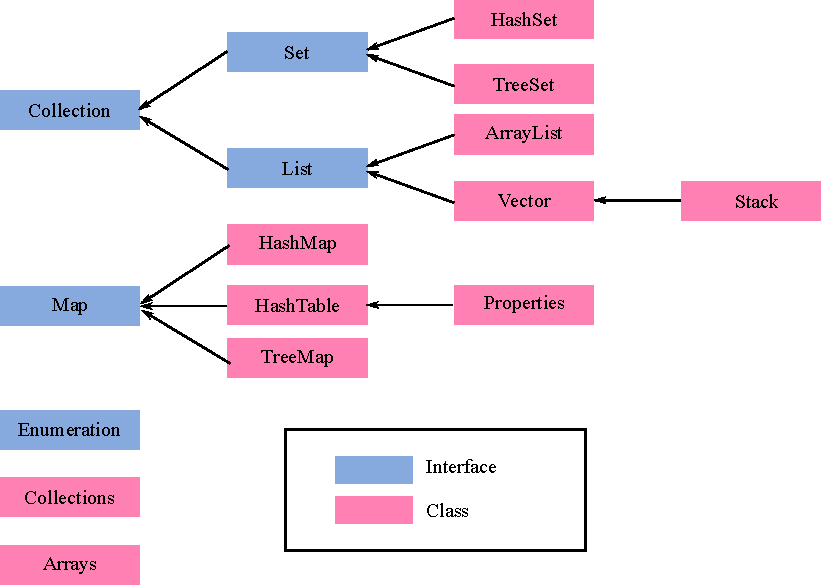
\includegraphics[width=0.8\textwidth]{fig-set-list-map.pdf}
  \end{figure}
\end{frame}


\section{Collection和Map接口}

\begin{frame}[fragile] % [fragile]参数使得能够插入代码
  \frametitle{Collection接口}

  java.util.Collection接口是描述Set和List集合类型(不包含Map)的根接口,
  其中定义了有关集合操作的普遍性方法:
  
  \begin{itemize}[<+-| alert@+>]
  \item boolean add(Object o)\\
    \only<1>{向集合中添加一个元素,在子接口中此方法发生了分化,如Set接口
      中添加重复元素时会被拒绝(返回false,而不是出错);List接口则会接受
      重复元素且返回true。}
  \item boolean remove(Object o) \\
    \only<2>{从集合中移除指定的元素。}
  \item int size()\\
    \only<3>{返回集合中元素的数目。}
  \item boolean isEmpty()\\
    \only<4>{判断集合是否为空(即是否包含任何元素)。}
  \item boolean contains(Object o) \\
    \only<5>{判断集合中是否包含指定的元素。}
  \item void clear()\\
    \only<6>{移除当前集合中的所有元素。}
  \item Iterator iterator()\\
    \only<7>{返回在此集合的元素上进行迭代的迭代器。}
  \item Object[] toArray()\\
    \only<8>{返回包含当前集合中所有元素的数组。}
  \end{itemize}
\end{frame}

\begin{frame}[fragile] % [fragile]参数使得能够插入代码
  \frametitle{Set和List接口}

  java.util.Set和java.util.List分别描述前述的集和列表结构,二者均
  为Collection的子接口。

  \pause
  
  {\kai Set接口模拟了数学意义的集合。List接口规定使用者可以对列表元素的插入位置
    进行精确控制,并添加了根据元素索引来访问元素等功能,接口中新添加了相应
    方法:}

  \begin{itemize}[<+-| alert@+>]\kai
  \item void add(int index, Object element)
  \item Object get(int index)
  \item Object set(int index, Object element) 
  \item int indexOf(Object o) 返回列表中首次出现指定元素的索引,如果列表不包含指定元素,则返回-1。
  \item Object remove(int index)
  \end{itemize}
\end{frame}

\begin{frame}[fragile] % [fragile]参数使得能够插入代码
  \frametitle{Map接口}

  java.util.Map接口描述了映射结构,Map结构允许以{\hei\Blue 键集、值集合
    或键—值映射关系集}的形式查看某个映射的内容。主要方法:
  
  \begin{itemize}[<+-| alert@+>]\kai
  \item Object put(Object key, Object value)\\
    \only<1>{向当前映射中加入一组新的健—值对,并返回所加入元素的“值”,如果此映射中以前包含一个该键的映射关系,则用新值替换旧值。}
  \item Object get(Object key)\\
    \only<2>{返回此映射中映射到指定键的值,没有则返回null。}
  \item boolean isEmpty()
  \item void clear()
  \item int size()
  \item boolean containsKey(Object key)\\
    \only<6>{如果映射中包含指定键的映射关系,则返回true,否则返回false。}
  \item boolean containsValue(Object value)
  \item Set keySet()\\
    \only<8>{返回此映射中包含的键的set视图,此Set受映射支持,所以对映射的改变可以在此Set中反映出来,反之亦然。}
  \item Collection values()\\
    \only<9>{返回此映射包含值的Collection视图,此Collection受映射支持,所以对映射的改变可以在此Collection中反映出来,反之亦然。}
  \end{itemize}
\end{frame}

\section{列表}

\begin{frame}[fragile] % [fragile]参数使得能够插入代码
  \frametitle{ArrayList类}

  java.util.ArrayList类实现了List接口,用于表述长度可变的数组列表。

  ArrayList列表允许元素取值为null。除实现了List接口定义的所有功能外,还提供了一些方法来操作列表容量的大小,相关方法包括:

  \begin{itemize}\kai
  \item public ArrayList()\\构造方法:创建一个初始容量为10的空列表。
  \item public ArrayList(int initialCapacity)
  \item {\Red public void ensureCapacity(int minCapacity)\\对容器进行扩容。}
  \item public void trimToSize() \\将此ArrayList实例的容量调整为列表的当前大小。
  \end{itemize}
\end{frame}

\begin{frame}[fragile]
  \frametitle{代码的局部性能优化 ensureCapacity}

  \wxd{ArrayList ensureCapacity(int n)}

  \begin{itemize}\kai
  \item 该方法可以对ArrayList底层的数组进行扩容。
  \item 显示的调用这个函数,如果参数大于低层数组长度的1.5倍,那么这个数
    组的容量就会被扩容到这个参数值,如果参数小于低层数组长度的1.5倍,那
    么这个容量就会被扩容到低层数组长度的1.5倍。
  \item 在适当的时机,好好利用这个函数,将会使我们写出来的程序性能得到
    很大的提升。
  \end{itemize}

  \codeset{sample.setlistmap.ArrayListEnSureCapacitySample.java}
\end{frame}

\begin{frame}[fragile] % [fragile]参数使得能够插入代码
  \frametitle{Vector类}

  java.util.Vector也实现了List接口,其描述的也是可变长度的对象数组。

  \wxd{与ArrayList的差别}

  {\Red\kai Vector是同步(线程安全)的,运行效率要低一些,主要用在在多线
    程环境中,而ArrayList是不同步的,适合在单线程环境中使用。}

  常用方法(除实现List接口中定义的方法外):

  \begin{itemize}\small
  \item public Vector()
  \item public Object elementAt(int index)
  \item public void addElement(Object obj)
  \item public void removeElementAt(int index)
  \item public void insertElementAt(E obj, int index) 
  \item public boolean removeElement(Object obj) 
  \item public void removeAllElements()
  \item public Object[] toArray()
  \end{itemize}
\end{frame}

\begin{frame}[fragile]
  \frametitle{何谓线程安全}

  \wxd{线程安全的一般意义}

  \begin{description}\kai\small
  \item[线程安全] 在多线程访问时采用加锁机制,当一个线程访问该类的某个
    数据时进行保护,其他线程不能进行访问直到该线程读取完,其他线程才可
    使用,不会出现数据不一致或者数据污染。(Vector、HashTable等)
  \item[线程不安全] 不提供数据访问保护,有可能出现多个线程先后更改数据导致出现“脏数据”。
    (ArrayList、LinkedList、HashMap等)
  \end{description}

  \begin{figure}
    \centering
    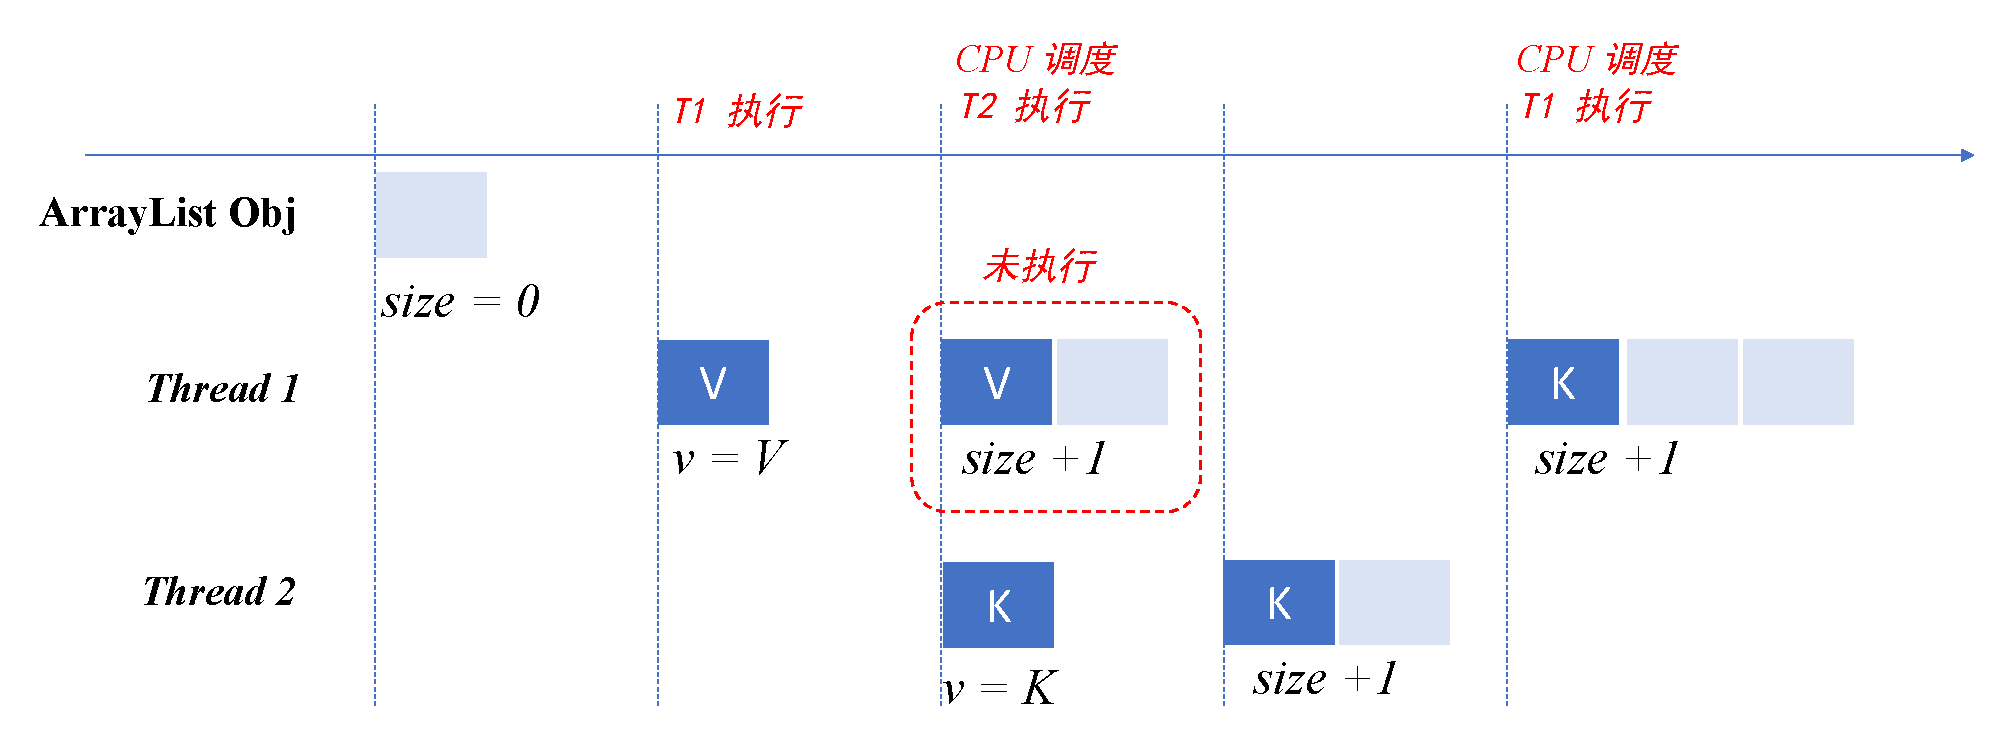
\includegraphics[width=0.85\textwidth]{thread-safe.pdf}
  \end{figure}

  %%% 比如一个 ArrayList 类,在添加一个元素的时候,它可能会有两步来完
  %%% 成:1. 在 Items[Size] 的位置存放此元素;2. 增大 Size 的值。 在单线程
  %%% 运行的情况下,如果 Size = 0,添加一个元素后,此元素在位置 0,而
  %%% 且 Size=1; 而如果是在多线程情况下,比如有两个线程,线程 A 先将元素存
  %%% 放在位置 0。但是此时 CPU 调度线程A暂停,线程 B 得到运行的机会。线
  %%% 程B也向此 ArrayList 添加元素,因为此时 Size 仍然等于 0 (注意哦,我们
  %%% 假设的是添加一个元素是要两个步骤哦,而线程A仅仅完成了步骤1),所以线
  %%% 程B也将元素存放在位置0。然后线程A和线程B都继续运行,都增加 Size 的
  %%% 值。 那好,我们来看看 ArrayList 的情况,元素实际上只有一个,存放在位
  %%% 置 0,而 Size 却等于 2。这就是“线程不安全”了。
\end{frame}

\begin{frame}[fragile] % [fragile]参数使得能够插入代码
  \frametitle{Stack} java.util.Stack类继承了Vector类,对应数据结构中
  以{\hei\Blue “后进先出”(Last in First out, LIFO)方式存储和操作数
    据的对象栈}。Stack类提供了常规的栈操作方法:

  \begin{itemize}\kai\small
  \item public Stack() 构造方法,创建一个空栈。
  \item public Object push(E item) 向栈中压入数据。
  \item public Object pop() 移除栈顶对象并作为此方法的返回值。
  \item public Object peek() 查看/返回栈顶对象,但不从栈中移除它。
  \item public boolean empty() 测试栈是否为空。
  \item public void clear() 清空栈。
  \item public int search(Object o) 返回对象在栈中的位置,以1为基数。
  \end{itemize}
\end{frame}

\section{Iterator接口}

\begin{frame}[fragile] % [fragile]参数使得能够插入代码
  \frametitle{Iterator接口}

  \wxd{统一的遍历方式}
  
  \begin{itemize}
  \item 对于ArrayList可以使用get()方法访问其元素;
  \item 对于Vector,还可以使用elmentAt()方法访问其元素;
  \item 后续Set和Map集合也有各自不同的元素访问方式。
  \end{itemize}
  \pause {\Blue\hei 是否有一种统一的方式来遍历各种不同类型集合中的元素呢?}

\end{frame}

\begin{frame}[fragile] % [fragile]参数使得能够插入代码
  \frametitle{Iterator接口}

  Java.util.Iterator接口描述的是以统一方式对各种集合元素进行遍历/迭代的工具,也称为“{\Blue\hei 迭代器}”。

  迭代器允许在遍历过程中移除集合中的(当前遍历到的那个)元素。主要方法包括:

  \begin{itemize}\small\kai
  \item boolean hasNext()\\
    如果仍有元素可以迭代,则返回true,否则返回false。
  \item Object next()\\
    返回迭代的下一个元素,重复调用此方法直到haseNext()方法返回false。
  \item void remove()\\
    将当前迭代到的元素从迭代器指向的集合中移除。
  \end{itemize}
\end{frame}

\begin{frame}[fragile] % [fragile]参数使得能够插入代码
  \frametitle{使用迭代器}

  我们一般不直接创建迭代器对象,而是通过调用集合对象的iterator()方法(该方法在Collection接口中定义)来获取。

  \samp{TestIterator.java}

  \begin{javaCode}
    import java.util.ArrayList;
    import java.util.Iterator;

    public class TestIterator {
      public static void main(String[] args) {
        ArrayList a = new ArrayList();
        a.add("China");
        a.add("USA");
        a.add("Korea");
        Iterator it = a.iterator();
        
        while(it.hasNext()) {
          String country = (String) it.next();
          System.out.println(country);
        }
      }
    }
  \end{javaCode}
  {\kai\Red 注意:迭代器相当于原始集合的一个“视图”,即一种表现形式,而不是复制其中所有元素得到的拷贝,因此在迭代器上的操作将影响到原来的集合。}
\end{frame}

\section{集}

\begin{frame}[fragile] % [fragile]参数使得能够插入代码
  \frametitle{HashSet类}

  java.util.HashSet类实现了java.util.Set接口,描述典型的Set集合结构。

  \begin{itemize}
  \item HashSet中不允许出现重复元素,不保证集合中元素的顺序。
  \item HashSet中允许包含值为null的元素,但最多只能有一个null元素。
  \end{itemize}
\end{frame}

\begin{frame}[fragile] % [fragile]参数使得能够插入代码
  \frametitle{TreeSet类}

  java.util.TreeSet类也实现了java.util.Set,它描述的是Set的一种变体——可以
  实现排序功能的集合。

  \begin{itemize}\kai
  \item 在将对象元素添加到TreeSet集中时会自动按照某种比较规则将其插入到有
    序的对象序列中,以保证TreeSet集合元素组成的对象序列时刻按照“升序”排
    列(例如按照字典顺序排列);
  \item 对于用户自定义的类型的数据可以自行定义其所需的排序规则(使用Comparable接口)。
  \end{itemize}
\end{frame}

\begin{frame}[fragile] % [fragile]参数使得能够插入代码
  \frametitle{Comparable接口}

  java.lang.Comparable接口中定义的compareTo()方法用于提供对其实现类的对象
  进行整体排序所需的比较逻辑,所为的排序可以理解为按照某种标准来比较对象
  的大小以确定其次序。

  \begin{itemize}\kai
  \item 实现类基于compareTo()方法的排序被称为{\Blue 自然排序}。
  \item compareTo()方法被称为它的{\Blue 自然比较方法},具体的排序原则可由实现类根据需要而定。
  \end{itemize}

  \xyy{方法格式}
  \begin{javaCode}
    int compareTo(Object o) {
      
    }   
  \end{javaCode}

  \samp{sample.setlistmap.NatrualOrderingSample.java}
  
\end{frame}

\begin{frame}[fragile] % [fragile]参数使得能够插入代码
  \frametitle{Comparable接口}

  \wxd{使用Comparable接口实现自然排序}
  \samp{Person.java}
  \begin{javaCode}
    public class Person implements java.lang.Comparable {
      private final int id;
      ...

      public Person(int id, String name, int age) {
        this.id = id;
        ...
      }
      ...
      @Override
      public int compareTo(Object o) {
        Person p = (Person) o;
        return this.id - p.id;
      }
      @Override
      public boolean equals(Object o) {
        boolean flag = false;
        if (o instanceof Person) {
          if (this.id == ((Person) o).id) {
            flag = true;
          }
        }
        return flag;
      }
    } 
  \end{javaCode}
\end{frame}

\begin{frame}[fragile] % [fragile]参数使得能够插入代码
  \frametitle{Comparable接口}

  \samp{TestComparable.java}

  \begin{javaCode}
    import java.util.TreeSet;
    import java.util.Iterator;

    public class TestComparable {
      public static void main(String[] args) {
        TreeSet ts = new TreeSet();
        ts.add(new Person(1003, "Bob", 15));
        ts.add(new Person(1008, "Alice", 25));
        ts.add(new Person(1001, "Kevin", 30));
      }
      Iterator it = ts.iterator();
      while (it.hasNext()) {
        Person emplyee  = (Person) it.next();
        System.out.println(employee);
      }
    }
  \end{javaCode}

  \begin{stdoutCode}
    Id: 1001 Name: Kevin Age:30
    Id: 1003 Name: Bob Age:15
    Id: 1008 Name: Alice Age:25
  \end{stdoutCode}
\end{frame}

\begin{frame}[fragile] % [fragile]参数使得能够插入代码
  \frametitle{Comparable接口}

  \wxd{对上述程序的几点说明}

  \begin{enumerate}[<+-| alert@+>]\kai
  \item 用户在重写compareTo()方法以定制比较逻辑时,需要确保其与等价性判断
    方法equals()保持一致,即确保条件“{\Red (x.compareTo(y) == 0) ==
      (x.equals(y))}”永远成立,否则逻辑上不合理。所以上例同时重写
    了equals()方法。
  \item 为保证能够实现元素的排序功能,TreeSet集合要求向其加入的对象元素必
    须是Comparable接口的实现类的实例,否者程序运行时会抛出{\Red 造型异常}。
    % (java.lang.ClassCastException)。
  \item Comparable接口并不专用于集合框架。
  \end{enumerate}
\end{frame}

\section{映射}

\begin{frame}[fragile] % [fragile]参数使得能够插入代码
  \frametitle{HashMap类}

  java.util.HashMap类实现了java.util.Map接口,该类基于{\hei\Blue 哈希表}实现了前述的映射集合结构。

  \begin{itemize}\kai
  \item HashMap结构不保证其中元素(映射信息)的先后顺序,且允许使用null“值”和null“键”。
  \item 当集合中不存在当前检索的“键”所对应的映射值时,HashMap的get()方法会返回空值null,而不会运行出错。
  \item 影响HashMap性能的两个参数:初始容量(Initial Capacity)和加载因子(Load Factor)。
  \end{itemize}
\end{frame}

\begin{frame}[fragile] % [fragile]参数使得能够插入代码
  \frametitle{HashTable类}

  java.util.Hashtable与HashMap作用基本相同,也实现了Map接口,采用哈希表的方式将“键”映射到相应的“值”。

  \wxd{Hashtable与HashMap的差别}

  \begin{itemize}\kai
  \item Hashtable中元素的“键”和“值”均不允许为null,而HashMap则允许。
  \item {\Red Hashtable是同步的,即线程安全的,效率相对要低一些,适合在多
      线程环境下使用;而 HashMap是不同步的,效率相对高一些,提倡在单线程
      环境中使用。}
  \item 除此之外,Hashtable与HashMap的用法格式完全相同。
  \end{itemize}
\end{frame}

\begin{frame}[fragile] % [fragile]参数使得能够插入代码
  \frametitle{TreeMap类}

  java.util.TreeMap类实现了将Map映射中的元素按照“键”进行升序排列的功能,其排序规则可以是默
  认的按照“键”的自然顺序排列,也可以使用指定的其他排序规则。

  向TreeMap映射中添加的元素“键”所属的类必须实现Comparable接口。

  \begin{javaCode}
    public MyKey implements Comparable {
      private final int id;
      ...
      public MyKey(int id) {
        this.id = id;
      }
      ...
      @Override
      public int compareTo(Object o) {
        return this.id - ((MyKey) o).id;
      }
      @Override
      public boolean equals(Object o) {
        return (o instanceof MyKey) && (this.id == ((MyKey) o).id);
      }
      @Override
      public int hashCode() {
        return new Integer(id).hasCode();
      }
    }  
  \end{javaCode}
\end{frame}

\begin{frame}[fragile] % [fragile]参数使得能够插入代码
  \frametitle{TreeMap类}
  \wxd{对上述程序的说明}

  {\kai MyKey类重写equals()方法的同时也重写了hasCode()方法,这是一种规
    范的做法,目的是为了维护hasCode()方法的常规协定,该协定要求相等对象
    必须具有相等的哈希码,即当两个对象使用equals()方法比较结果为等价时,
    它们各自调用hasCode()方法也应该返回相同的结果。}
\end{frame}

\section{其他相关API}
\begin{frame}[fragile] % [fragile]参数使得能够插入代码
  \frametitle{Enumeration接口}

  \xyy{java.util.Enumeration} 接口作用与Iterator接口类似,但只提供了遍
  历Vector和Hashtable(及子类Properties)类型集合元素的功能,且不支持集
  合元素的移除操作。

  \begin{javaCode}
    import java.util.*;

    public class TestEnumeration {
      public static void main(String[] args) {
        Vector v = new Vector();
        v.addElement("Lisa");
        v.addElement("Billy");
        v.addElement("Brown");

        Enumeration e = v.elements();

        while(e.hasMoreElements()) {
          String value = (String) e.nextElement();
          System.out.println(value);
        }
      }
    }
  \end{javaCode}
\end{frame}

\begin{frame}[fragile] % [fragile]参数使得能够插入代码
  \frametitle{Collections类}

  \xyy{java.util.Collections} 类定义了多种集合操作方法,能够实现了对集
  合元素的{\Blue\hei 排序、取极值、批量拷贝、集合结构转换、循环移位以及
    匹配性检查}等功能。Collections类的主要方法包括:

  \begin{itemize}\small
  \item public static void sort(List list)
  \item public static void reverse(List list)
  \item public static void shuffle(List list)
  \item public static void copy(List dest, List src)
  \item public static ArrayList list(Enumeration e)
  \item public static int frequency(Collection c, Object o)
  \item public static T max(Collection coll)
  \item public static T min(Collection coll)
  \item public static void rotate(List list, int distance)
  \end{itemize}
\end{frame}

\begin{frame}[fragile] % [fragile]参数使得能够插入代码
  \frametitle{Arrays类}

  \xyy{java.util.Arrays} 类定义了多种数组操作方法,实现了对数组元素的排
  序、填充、转换为列表或字符串形式、增强的检索和深度比较等功
  能。Arrays类的主要方法包括\footnote{自行搜索学习各方法的用法}:

  \begin{itemize}
  \item public static List asList(Object... a)
  \item public static void sort(<类型>[ ] a)
  \item public static int binarySearch(int[] a, int key)
  \item public static String toString(int[] a)
  \end{itemize}
\end{frame}


\begin{frame}[fragile]
  \frametitle{本节习题}

  \wxd{简答题}
  \begin{enumerate}
  \item 根据本节内容,自行梳理一张Java集合与映射的思维导图(使用xmind
    8等思维导图工具),包含分类结构、概念及用法解释,越详细越好。{\kai
      (注意:网上有很多,大家可以参考但思维导图必须自己来画)}
  \end{enumerate}
  
  \wxd{小编程}
  
  \begin{enumerate}
  \item 写代码学习掌握各种常用集合容器类型及容器操作API的使用方法。
  \end{enumerate}

\end{frame}


% TKS %%%%%%%%%%%%%%%%%%%%%%%%%%%%%%%%%%%%%%%%%%%%%%
\begin{frame}[focus]
  \centering
  {\Huge {THE END}} \\
  \vspace{5mm}
  {\Large wangxiaodong@ouc.edu.cn} \\
\end{frame}
%%%%%%%%%%%%%%%%%%%%%%%%%%%%%%%%%%%%%%%%%%%%%%%%%%%% 
\end{document}

% Week 06 %%
%%%%%%%%%%%%%%%%%%%%%%%%%%%%%%%%%%%%%%%%%%%%%%%%%%%%%%%%%%%%%%%%%%%%%%%%%%%%%%%
\documentclass[hyperref={pdfpagelabels=false},compress,table]{beamer} % 在Mac下无法编译
% \documentclass[compress,table]{beamer} % 在Mac下使用
% package for font
\usepackage{fontspec}
\defaultfontfeatures{Mapping=tex-text}  %%如果没有它,会有一些 tex 特殊字符无法正常使用,比如连字符。
\usepackage{xunicode,xltxtra}
\usepackage[BoldFont,SlantFont,CJKnumber,CJKchecksingle]{xeCJK}  % \CJKnumber{12345}: 一万二千三百四十五
\usepackage{CJKfntef}  %%实现对汉字加点、下划线等。
\usepackage{pifont}  % \ding{}
% package for math
\usepackage{amsfonts}

% package for graphics
\usepackage[americaninductors,europeanresistors]{circuitikz}
\usepackage{tikz}
\usetikzlibrary{plotmarks}  % placements=positioning
\usepackage{graphicx}  % \includegraphics[]{}
\usepackage{subfigure}  %%图形或表格并排排列
% package for table
\usepackage{colortbl,dcolumn}  %% 彩色表格
\usepackage{multirow}
\usepackage{multicol}
\usepackage{booktabs}
% package for code
\usepackage{fancyvrb}
\usepackage{listings}

% \usepackage{animate}
% \usepackage{movie15}

%%%%%
% setting for beamer
\usetheme{default} % Madrid(常用), Copenhagen, AnnArbor, boxes(白色), Frankfurt,Berkeley
\useoutertheme[subsection=true]{miniframes} % 使用Berkeley时注释本行
\usecolortheme{sidebartab}
\usefonttheme{serif}  %%英文使用衬线字体
% \setbeamertemplate{background canvas}[vertical
% shading][bottom=white,top=structure.fg!7] %%背景色,上25%的蓝,过渡到下白。
\setbeamertemplate{theorems}[numbered]
\setbeamertemplate{navigation symbols}{}  %% 去掉页面下方默认的导航条
\setbeamercovered{transparent}  %设置 beamer 覆盖效果

% 设置标题title背景色
% \setbeamercolor{title}{fg=black, bg=lightgray!60!white}
\setbeamercolor{title}{fg=white, bg=black!70!white}

% 设置每页小LOGO
\pgfdeclareimage[width=1cm]{ouc}{figures/static/ouc.pdf}
\logo{\pgfuseimage{ouc}{\vspace{-20pt}}}

% setting for font
%%\setCJKmainfont{Adobe Kaiti Std}
\setCJKmainfont{SimSun} 
%% \setCJKmainfont{FangSong_GB2312} 
%% \setmainfont{Apple Garamond}  %%苹果字体没有SmallCaps
\setCJKmainfont{SimSun} 
%FUNNY%\setCJKmainfont{DFPShaoNvW5-GB}  %%华康少女文字W5(P)
%FUNNY%\setCJKmainfont{FZJingLeiS-R-GB}  %%方正静蕾体
%FUNNY%\setmainfont{Purisa}
%\setsansfont[Mapping=tex-text]{Adobe Song Std}
     %如果装了Adobe Acrobat,可在font.conf中配置Adobe字体的路径以使用其中文字体。
     %也可直接使用系统中的中文字体如SimSun、SimHei、微软雅黑等。
     %原来beamer用的字体是sans family;注意Mapping的大小写,不能写错。
     %设置字体时也可以直接用字体名,以下三种方式等同:
     %\setromanfont[BoldFont={黑体}]{宋体}
     %\setromanfont[BoldFont={SimHei}]{SimSun}
     %\setromanfont[BoldFont={"[simhei.ttf]"}]{"[simsun.ttc]"}
% setting for graphics
\graphicspath{{figures/}}  %%图片路径
\renewcommand\figurename{图}

% setting for pdf
\hypersetup{% pdfpagemode=FullScreen,%
            pdfauthor={Xiaodong Wang},%
            pdftitle={Title},%
            CJKbookmarks=true,%
            bookmarksnumbered=true,%
            bookmarksopen=false,%
            plainpages=false,%
            colorlinks=true,%
            citecolor=green,%
            filecolor=magenta,%
            linkcolor=blue,%red(default)
            urlcolor=cyan}

% setting for fontspec
\XeTeXlinebreaklocale "zh"  %%表示用中文的断行
\XeTeXlinebreakskip = 0pt plus 1pt minus 0.1pt  %%多一点调整的空间
%%%%%

% font setting by xeCJK
\setCJKfamilyfont{NSimSun}{NSimSun}
\newcommand{\song}{\CJKfamily{NSimSun}}
%%%\setCJKfamilyfont{AdobeSongStd}{Adobe Song Std}
%%%\newcommand{\AdobeSong}{\CJKfamily{AdobeSongStd}}
\setCJKfamilyfont{FangSong}{FangSong_GB2312}
\newcommand{\fang}{\CJKfamily{FangSong}}
%%%\setCJKfamilyfont{AdobeFangsongStd}{Adobe Fangsong Std}
%%%\newcommand{\AdobeFang}{\CJKfamily{AdobeFangsongStd}}
\setCJKfamilyfont{SimHei}{SimHei}
\newcommand{\hei}{\CJKfamily{SimHei}}
%%%\setCJKfamilyfont{AdobeHeitiStd}{Adobe Heiti Std}
%%%\newcommand{\AdobeHei}{\CJKfamily{AdobeHeitiStd}}
\setCJKfamilyfont{KaiTi}{KaiTi}
\newcommand{\kai}{\CJKfamily{KaiTi}}
%%%\setCJKfamilyfont{AdobeKaitiStd}{Adobe Kaiti Std}
\newcommand{\AdobeKai}{\CJKfamily{AdobeKaitiStd}}
\setCJKfamilyfont{LiSu}{LiSu}
\newcommand{\li}{\CJKfamily{LiSu}}
\setCJKfamilyfont{YouYuan}{YouYuan}
\newcommand{\you}{\CJKfamily{YouYuan}}
\setCJKfamilyfont{FZJingLei}{FZJingLeiS-R-GB}
\newcommand{\jinglei}{\CJKfamily{FZJingLei}}
\setCJKfamilyfont{MSYH}{Microsoft YaHei}
\newcommand{\msyh}{\CJKfamily{MSYH}}

% 自定义颜色
\def\Red{\color{red}}
\def\Green{\color{green}}
\def\Blue{\color{blue}}
\def\Mage{\color{magenta}}
\def\Cyan{\color{cyan}}
\def\Brown{\color{brown}}
\def\White{\color{white}}
\def\Black{\color{black}}

\lstnewenvironment{xmlCode}[1][]{% for Java
  \lstset{
    basicstyle=\tiny\ttfamily,%
    columns=flexible,%
    framexleftmargin=.7mm, %
    % frame=shadowbox,%
    % rulesepcolor=\color{cyan},%
     frame=single,%
    backgroundcolor=\color{white},%
    xleftmargin=4\fboxsep,%
    xrightmargin=4\fboxsep,%
    numbers=left,numberstyle=\tiny,%
    numberblanklines=false,numbersep=7pt,%
    language=xml, %
    }\lstset{#1}}{}

\lstnewenvironment{javaCode}[1][]{% for Java
  \lstset{
    basicstyle=\tiny\ttfamily,%
    columns=flexible,%
    framexleftmargin=.7mm, %
    frame=shadowbox,%
    rulesepcolor=\color{cyan},%
    % frame=single,%
    backgroundcolor=\color{white},%
    xleftmargin=4\fboxsep,%
    xrightmargin=4\fboxsep,%
    numbers=left,numberstyle=\tiny,%
    numberblanklines=false,numbersep=7pt,%
    language=Java, %
    }\lstset{#1}}{}

\lstnewenvironment{shCode}[1][]{% for Java
  \lstset{
    basicstyle=\scriptsize\ttfamily,%
    columns=flexible,%
    framexleftmargin=.7mm, %
    frame=shadowbox,%
    rulesepcolor=\color{brown},%
    % frame=single,%
    backgroundcolor=\color{white},%
    xleftmargin=4\fboxsep,%
    xrightmargin=4\fboxsep,%
    numbers=left,numberstyle=\tiny,%
    numberblanklines=false,numbersep=7pt,%
    language=sh, %
    }\lstset{#1}}{}

\newcommand\ask[1]{\vskip 4bp \tikz \node[rectangle,rounded corners,minimum size=6mm,
  fill=white,]{\Cyan \includegraphics[height=1.5cm]{question} \Large \msyh #1};}

\newcommand\wxd[1]{\vskip 4bp \tikz \node[rectangle,minimum size=6mm,
  fill=blue!60!white,]{\White \ding{118} \msyh #1};}

\newcommand\xyy[1]{\vskip 2bp \tikz \node[rectangle,minimum size=3mm,
  fill=black!80!white,]{\White \msyh\scriptsize #1};}

\newcommand\cxf[1]{\vskip 4bp \tikz \node[rectangle,rounded corners,minimum size=6mm,
  fill=orange!60!white,]{\White \ding{42} \msyh #1};}

\newcommand\samp[1]{\vskip 2bp \tikz \node[rectangle,minimum size=3mm,
  fill=white!100!white,]{\Mage\msyh \small CODE \ding{231} \Black #1};\vskip -8bp}

\newcommand\zhyfly[1]{\tikz \node[rectangle,rounded corners,minimum size=6mm,ball color=red!25!blue,text=white,]{#1};}

\setbeamerfont{frametitle}{series=\msyh} % 修改Beamer标题字体

\makeatletter
\newcommand{\Extend}[5]{\ext@arrow 0099{\arrowfill@#1#2#3}{#4}{#5}}
\makeatother


%%%%%%%%%%%%%%%%%%%%%%%%%%%%%%%%%%%%%%%%%%%%%%%%%%%%%%%%%%%%%%%%%%%%%%%%%%%%%%%
% \titlepage
\title[KevinW@OUC]{\hei {\huge Java 应用与开发}\\  
  GUI程序设计}
\author[王晓东]{王晓东\\
  \href{mailto:wangxiaodong@ouc.edu.cn}{\footnotesize wangxiaodong@ouc.edu.cn}}
\institute[中国海洋大学]{\small 中国海洋大学}
\date{\today}
\titlegraphic{\vspace{-6em}
\includegraphics[height=6cm]{static/ouc.pdf}\vspace{-6em}}
%%%%%
\begin{document}
%% Delete this, if you do not want the table of contents to pop up at
%% the beginning of each subsection:
\AtBeginSection[]{                              % 在每个Section前都会加入的Frame
  \frame<handout:0>{
    \frametitle{\textbf{\hei 接下来…}}
    \tableofcontents[currentsection]
  }
}  %

\AtBeginSubsection[]                            % 在每个子段落之前
{
  \frame<handout:0>                             % handout:0 表示只在手稿中出现
  {
    \frametitle{\textit{\hei 接下来…}}\small
    \tableofcontents[current,currentsubsection] % 显示在目录中加亮的当前章节
  }
}
\frame{\titlepage}
%%%%%%%%%%%%%%%%%%%%%%%%%%%%%%%%%%%%%%%%%%%%%%%%
\begin{frame}
  \frametitle{学习目标}
  \begin{enumerate}
  \item 了解用Java开发桌面软件图形用户界面的常用工具集
  \item 掌握AWT的常用组件和视觉控制
  \item 深入了解GUI事件处理机制
  \item 了解Applet,特别是其历史渊源,了解与Applet类似的技术
  \item 理解Swing和AWT的关系,学习使用Swing的典型组件构建较复杂的图形界面程序
  \end{enumerate}  
\end{frame}

\section*{大纲}
\frame{\frametitle{大纲} \tableofcontents }

\section{Java GUI设计}

\begin{frame}[fragile]
  \frametitle{用Java构建图形界面}

  \begin{itemize}
  \item AWT
  \item Swing
  \item JavaFX
  \end{itemize}
\end{frame}

\begin{frame}[fragile] % [fragile]参数使得能够插入代码
  \frametitle{概念和术语}

  \tta{图形用户界面}

  GUI (Graphical User Interface),Java主要分为AWT和Swing两大系列GUI API。

  \tta{抽象窗口工具集}

  AWT (Abstract Window Toolkit)

  \tta{相关软件包}

  \begin{description}
  \item[java.awt包] 提供基本GUI组件、视觉控制和绘图工具API。
  \item[java.awt.event包] 提供Java GUI事件处理API。
  \end{description}
\end{frame}

\begin{frame}[fragile] % [fragile]参数使得能够插入代码
  \frametitle{组件和容器}
  
  \begin{block}{组件}
    组件(Component)是图形用户界面的基本组成元素,凡是能够以图形化方式显示在屏幕上并能够与
    用户进行交互的对象均为组件,如菜单、按钮、标签、文本框、滚动条等。
  \end{block}

  \pause
  
  \begin{itemize}[<+-|alert@+>]\kai
  \item 组件不能独立地显示出来,必须将组件放在一定的容器中才可以显示出
    来。
  \item JDK的java.awt包中定义了多种GUI组件类,
    如Menu、Button、Label、TextField等。
  \item 抽象类java.awt.Component是除菜单相关组件之外所有Java AWT组件类
    的根父类,该类规定了GUI组件的基本特性,如尺寸、位置和颜色效果等,并
    实现了作为一个GUI部件所应具备的基本功能。
  \item java.awt.MenuComponent是所有与菜单相关的组件的父类。
  \end{itemize}
\end{frame}

\begin{frame}[fragile] % [fragile]参数使得能够插入代码
  \frametitle{组件和容器}
  
  \begin{block}{容器}
    容器(Container)实际上是Component的子类,容器类对象本身也是一个组
    件,具有组件的所有性质,另外还具有容纳其它组件和容器的功能。容器类
    对象可使用方法add()添加组件。
  \end{block}

  \pause
  
  \ttc{两种主要的容器类型}
  
  \begin{description}\kai
  \item[\fbox{java.awt.Window}] 可自由停泊的顶级窗口。
  \item[\fbox{java.awt.Panel}] 可作为容器容纳其他组件,但不能独立存在,必须被添加到其他容
    器(如Frame)中。
  \end{description}
\end{frame}

\begin{frame}[fragile] % [fragile]参数使得能够插入代码
  \frametitle{常用的组件和容器 \ding{182}}

  \begin{table}
    \scriptsize
    \setlength{\extrarowheight}{1.2mm}
    \rowcolors[]{1}{blue!30}{blue!10}
    \begin{tabular}{lll}
      {\bf 组件类型} & {\bf 父类}  & {\bf 说明}\\
      Button & Component & 可接收点击操作的矩形GUI组件\\
      Canvas & Component & 用于绘图的面板\\
      Checkbox & Component & 复选框组件\\
      CheckboxMenuItem & MenuItem & 复选框菜单项组件\\
      Choice & Component & 下拉式列表框,内容不可改变\\
      Component & Object & 抽象的组件类\\
      Container & Component & 抽象的容器类\\
      Dialog & Window & 对话框组件,顶级窗口、带标题栏\\
      FileDialog & Dialog & 用于选择文件的平台相关对话框\\
      Frame & Window & 基本的Java GUI窗口组件\\
      Label & Component & 标签类\\
    \end{tabular}
  \end{table}
\end{frame}

\begin{frame}[fragile] % [fragile]参数使得能够插入代码
  \frametitle{常用的组件和容器 \ding{183}}

  \begin{table}
    \scriptsize
    \setlength{\extrarowheight}{1.2mm}
    \rowcolors[]{1}{blue!30}{blue!10}
    \begin{tabular}{lll}
      {\bf 组件类型} & {\bf 父~类}  & {\bf 说~明}\\
      List & Component & 包含内容可变的条目的列表框组件\\
      MenuBar & MenuComponent & 菜单条组件\\
      Menu & MenuItem & 菜单组件\\
      MenuItem & MenuComponent & 菜单项组件\\
      Panel & Container & 基本容器类,不能单独停泊\\
      PopupMenu & Menu & 弹出式菜单组件\\
      Scrollbar & Component & 滚动条组件\\
      ScrollPane & Container & 带水平及垂直滚动条的容器组件\\
      TextComponent & Component & TextField和TextArea的基本功能\\
      TextField & TextComponent & 单行文本框\\
      TextArea & TextComponent & 多行文本域\\
      Window & Container & 抽象的GUI窗口类,无布局管理器\\
    \end{tabular}
  \end{table}
\end{frame}

\begin{frame}[fragile] % [fragile]参数使得能够插入代码
  \frametitle{Frame类}

  Frame类的显示效果是一个标准的图形窗口,它封装了GUI组件的各种属性信息,如尺寸、可见性等。

  \pause
  
  \begin{enumerate}\kai
  \item Frame对象的显示效果是一个可自由停泊的顶级“窗口”,带有标题和尺寸重置角标。
  \item Frame默认初始化为不可见的,可以调用Frame对象的setVisible(true)方法使之变为可见。
  \item 作为容器Frame还可使用add()方法包含其他组件。
  \end{enumerate}

  \codeset{sample.awt.FrameSample.java}
\end{frame}


\begin{frame}[fragile] % [fragile]参数使得能够插入代码
  \frametitle{组件定位}

  Java组件在容器中的定位由{\hei 布局管理器}决定。如要人工控制组件在容器中的定位,可取
  消布局管理器,然后使用Component类的下述成员方法设置:

  \begin{columns}
    \column{0.3\textwidth}
    \begin{itemize}
    \item setLocation()
    \item setSize()
    \item setBounds()
    \end{itemize}

    \column{0.8\textwidth}
    \begin{figure}
      \centering
      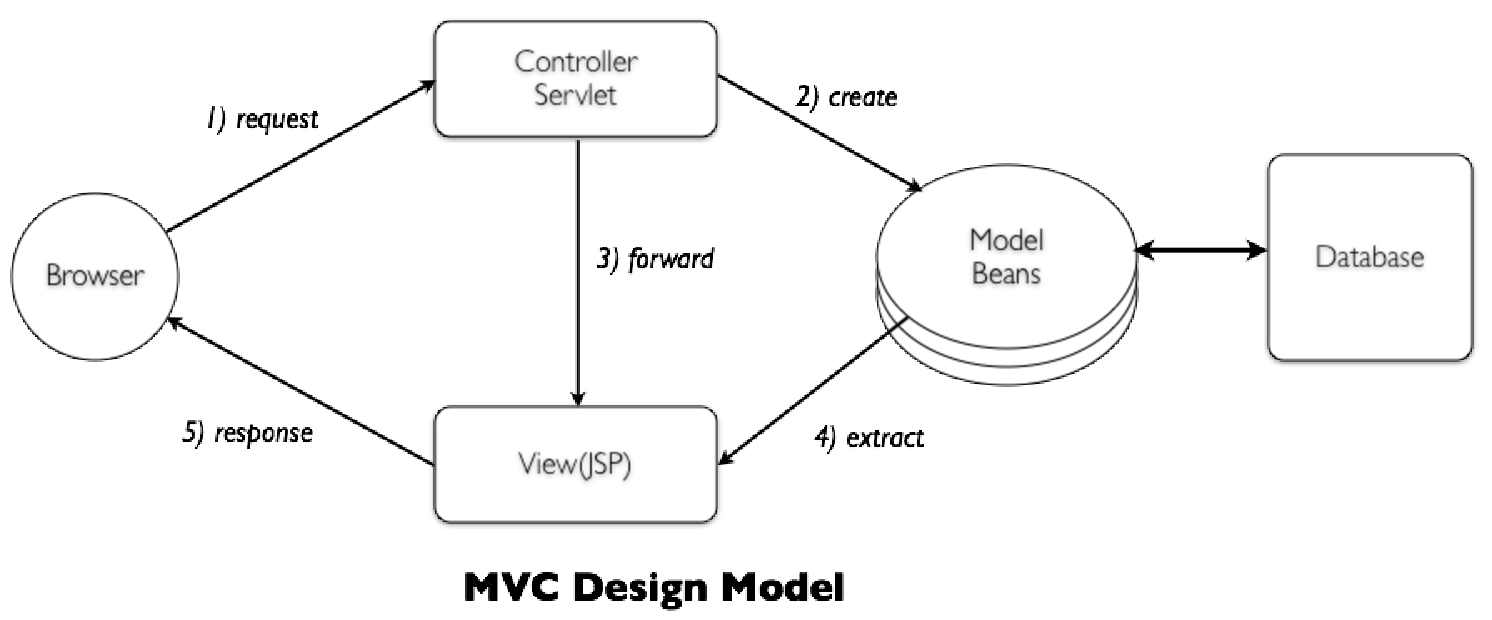
\includegraphics[width=1.0\textwidth]{fig02.pdf}
    \end{figure}
  \end{columns}

\end{frame}

\begin{frame}[fragile] % [fragile]参数使得能够插入代码
  \frametitle{Panel类}

  \begin{itemize}
  \item Panel提供容纳组件的空间。
  \item Panel不能独立存在,必须被添加到其他容器中。
  \item 可以采用和所在容器不同的布局管理器。
  \end{itemize}
  \codeset{sample.awt.FrameWithPanelSample.java}
\end{frame}

\begin{frame}[fragile] % [fragile]参数使得能够插入代码
\frametitle{布局管理器}

容器对其中所包含组件的排列方式,包括组件的位置和大小设定,被称为容器的布局(Layout)。

为了使图形用户界面具有良好的平台无关性,Java语言提供了布局管理器来管理容器的布局,而不建
议直接设置组件在容器中的位置和尺寸。

\ttc{布局管理器类层次}
{\small 
\begin{verbatim}
 LayoutManager----FlowLayout  
             |
             +----GridLayout

LayoutManager2----BorderLayout
             |
             +----CardLayout
             |
             +----GridBagLayout
\end{verbatim}}
注:LayoutManager2是LayoutManager的子接口。
\end{frame}

\begin{frame}[fragile] % [fragile]参数使得能够插入代码
  \frametitle{布局管理器}
  \begin{itemize}
  \item 每个容器都有一个布局管理器,当容器需要对某个组件进行定位或判断其大小尺寸时,就会调
    用其对应的布局管理器。
  \item 可以在容器创建后调用其setLayout()方法设置其布局管理器类型。
  \item Container类型容器没有默认的布局管理器,即其layoutMgr属性为null,在其子类中才进行分
    化。
  \end{itemize}
  \ttc{默认的布局管理器}
  \begin{figure}
    \centering
    \includegraphics[width=0.6\textwidth]{fig04.pdf}
  \end{figure}
\end{frame}

\begin{frame}[fragile] % [fragile]参数使得能够插入代码
  \frametitle{FlowLayout}

  \tta{流式布局} \\是Panel(及其子类)类型容器的默认布局管理器类型。

  \tta{布局效果}
  \begin{itemize}\kai
  \item 组件在容器中按照加入次序逐行定位,行内从左到右,一行排满后换行。
  \item 不改变组件尺寸,即按照组件原始大小进行显示。
  \item 组件间的对齐方式默认为居中对齐,也可在构造方法中设置不同的组件间距、行距及对齐方
    式。
  \end{itemize}
\end{frame}

\begin{frame}[fragile] % [fragile]参数使得能够插入代码
  \frametitle{FlowLayout}
  
  \tta{构造方法}
  \begin{itemize}\kai
  \item {\bf public FlowLayout()}\\
    组件对齐方式默认为居中对齐,组件的水平和垂直间距默认为5个像素。

  \item {\bf public FlowLayout(int align)}\\
    显式设定组件的对其方式,组件的水平和垂直间距默认为5个像素。\\
    FlowLayout.LEFT \\
    FlowLayout.RIGHT\\
    FlowLayout.CENTER\\

  \item {\bf public FlowLayout(int align, int hgap, int vgap)}\\
    显式设定组件的对其方式、组件的水平和垂直间距。
  \end{itemize}

  \codeset{sample.awt.layout.FlowLayoutSample.java}

\end{frame}


\begin{frame}[fragile] % [fragile]参数使得能够插入代码
\frametitle{BorderLayout}

\tta{边界布局} \\是Window及其子类(包括Frame、Dialog)容器的默认布局管理器。

\tta{布局效果}
\begin{itemize}
\item BorderLayout将整个容器的布局划分成东、西、南、北、中五个区域,组件只能被添加到指定
  的区域。如不指定组件的加入部位,则默认加入到Center区域。
\item 每个区域只能加入一个组件,如加入多个,则先前加入的组件会被遗弃。
\item 组件尺寸被强行控制,即与其所在区域的尺寸相同。
\end{itemize}
\end{frame}

\begin{frame}[fragile] % [fragile]参数使得能够插入代码
  \frametitle{BorderLayout}

  \tta{构造方法}
  
  \begin{itemize}\kai
  \item {\bf public BorderLayout()}\\
    构造一个BorderLayout布局管理器,其所包含的组件/区域间距为0。
  \item {\bf public BorderLayout(int hgap, int vgap)}\\
    构造一个BorderLayout布局管理器,根据参数的组件/区域间距。
  \end{itemize}

  \tta{BorderLayout型布局容器尺寸缩放原则}

  \begin{itemize}\kai
  \item 北、南两个区域只能在水平方向缩放(宽度可调整)。
  \item 东、西两个区域只能在垂直方向缩放(高度可调整)。
  \item 中部可在两个方向上缩放。
  \end{itemize}
\end{frame}

\begin{frame}[fragile] % [fragile]参数使得能够插入代码
  \frametitle{GridLayout}

  \tta{网格布局 - 布局效果}

  \begin{itemize}\small
  \item 将容器区域划分成规则的矩形网格,每个单元格区域大小相等,组件被添加到每个单元格
    中,按组件加入顺序先从左到右填满一行后换行,行间从上到下。
  \item GridLayout型布局的组件大小也被布局管理器强行控制,与单元格同等大小,当容器尺寸发
    生改变时,组件的相对位置保持不变,但大小自动调整。
  \end{itemize}

\end{frame}

\begin{frame}[fragile] % [fragile]参数使得能够插入代码
  \frametitle{GridLayout}
  
  \tta{构造方法}
  \begin{itemize}\kai
  \item {\bf public GridLayout()}  所有组件于一行中,各占一列。
  \item {\bf public GridLayout(int rows, int cols)}\\
    通过参数指定布局的行数和列数。
  \item {\bf public public GridLayout(int rows, int cols, int hgap, int vgap)}\\
    通过参数指定布局的行数、列数,以及组件间水平间距和垂直间距。
  \end{itemize}

  \codeset{sample.awt.layout.GridLayoutSample.java}
\end{frame}

\begin{frame}[fragile] % [fragile]参数使得能够插入代码
  \frametitle{CardLayout}

  \tta{布局效果}
  \begin{itemize}
  \item 将多个组件在同一容器区域内交替显示,相当于多张卡片摞在一起,只有最上面的卡片是可见
    的。
  \item 可以按名称显示某一张卡片,或按先后顺序依次显示,也可以直接定位到第一张或最后一张卡
    片。
  \end{itemize}

  \tta{主要方法}
  \begin{itemize}
  \item public void first(Container parent)
  \item public void last(Container parent)
  \item public void previous(Container parent)
  \item public void next(Container parent)
  \item public void show(Container parent, String name)
  \end{itemize}

  \codeset{sample.awt.layout.CardLayoutSample.java}
  
\end{frame}


\begin{frame}[fragile] % [fragile]参数使得能够插入代码
  \frametitle{容器的嵌套使用}

  利用容器嵌套可以在某个原本只能包含一个组件的区域中显示多个组件。

  \codeset{sample.awt.layout.FlowLayoutSample.java}
\end{frame}

\section{GUI事件处理}

\begin{frame}[fragile] % [fragile]参数使得能够插入代码
  \frametitle{Java事件和事件处理机制}

  从JDK 1.1开始,Java采用了一种名为“{\hei 事件代理模型}”(Event
  Delegation Model)的事件处理机制。基本原理如下:

  \begin{enumerate}\kai
  \item 事先定义多种事件类型
  \item 约定各种GUI组件在与用户交互时,遇到特定操作则会触发相应的事件,即自动创建事件类对象
    并提交给Java运行时系统
  \item 系统接收到事件类对象后,立即将其发送给专门的事件处理对象,该对象调用其事件处理方
    法,处理先前的事件类型对象,实现预期的处理逻辑
  \end{enumerate}
\end{frame}

\begin{frame}[fragile] % [fragile]参数使得能够插入代码
\frametitle{Java事件和事件处理机制}

若需要关注某个组件产生的事件,则可以在该组件上注册适当的事件处理方法,实际上注册的事件处
理者方法所属类型的一个对象——事件监听器。

\begin{figure}
\centering
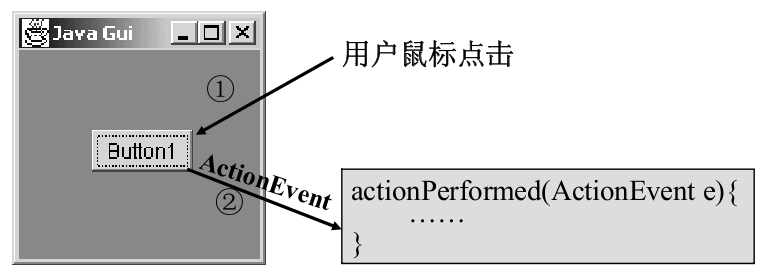
\includegraphics[width=0.8\textwidth]{fig10.png}
\end{figure}
\end{frame}

\begin{frame}[fragile] % [fragile]参数使得能够插入代码
\frametitle{事件处理相关概念}

\begin{description}[<+-|alert@+>]
\item[事件(Event)] 一个事件类型的对象,用于描述了发生什么事情,当用户在组件上进行操作时
  会触发相应的事件。
\item[事件源(Event Source)] 能够产生事件的GUI组件对象,如按钮、文本框等。
\item[事件处理方法(Event Handler)] 能够接收、解析和处理事件类对象,实现与用户交互功能的
  方法。
\item[事件监听器(Event Listener)] 调用事件处理方法的对象。
\end{description}

\codeset{sample.awt.event.ActionEventSample.java}

\end{frame}

\begin{frame}[fragile] % [fragile]参数使得能够插入代码
\frametitle{GUI事件类型层次}
\begin{figure}
\centering
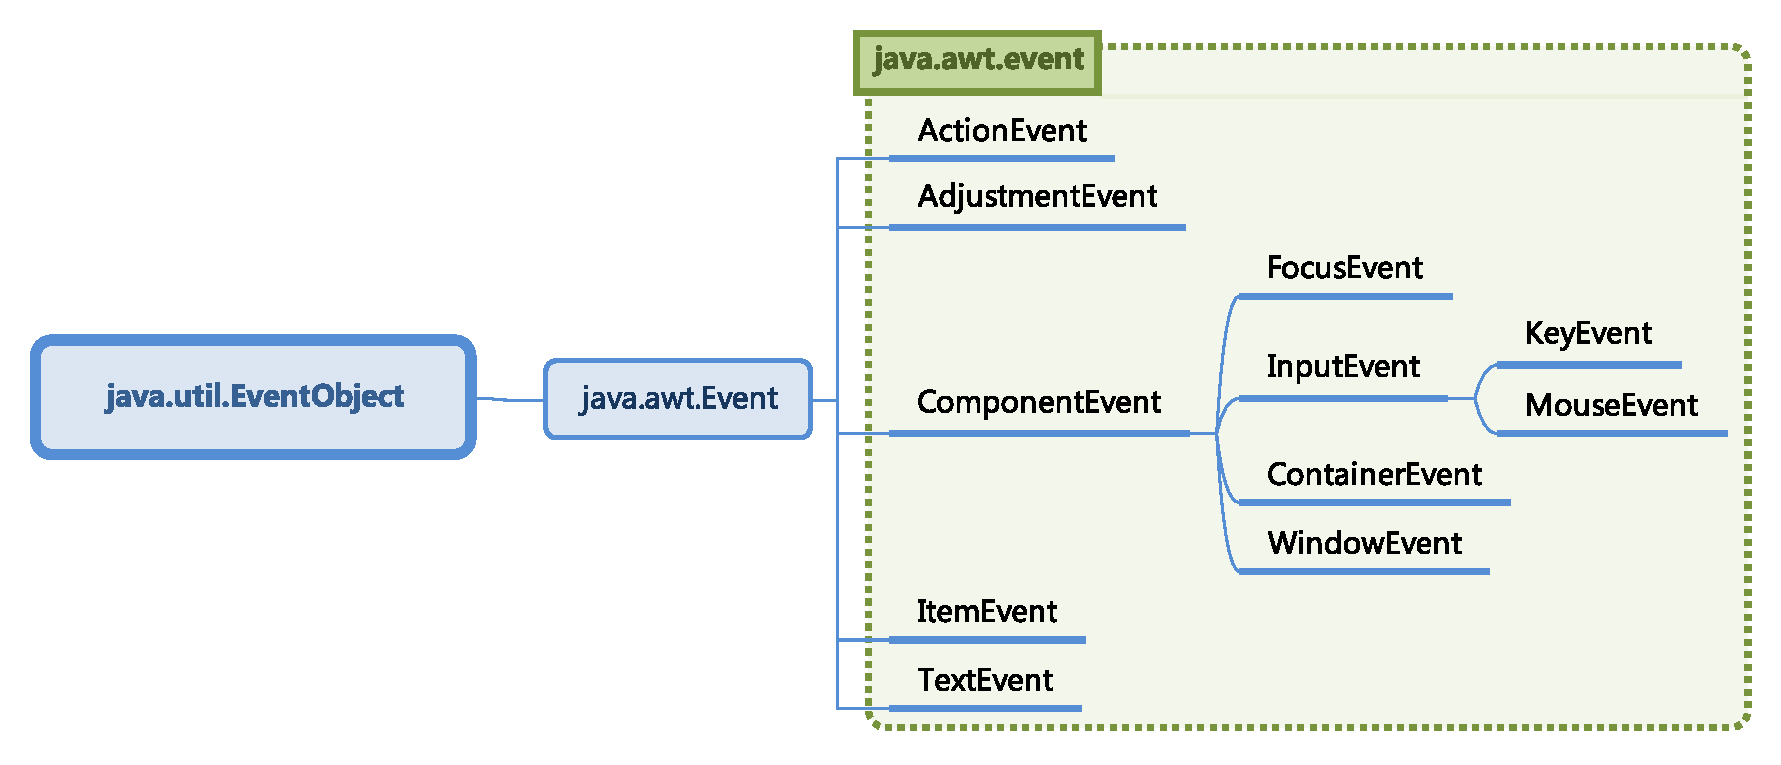
\includegraphics[width=\textwidth]{fig-awt-events.pdf}
\end{figure}
\end{frame}

\begin{frame}[fragile] % [fragile]参数使得能够插入代码
  \frametitle{GUI事件及相应监听器接口}
  \begin{table}
    \scriptsize
    \setlength{\extrarowheight}{1.2mm}
    \rowcolors[]{1}{blue!30}{blue!10}
    \begin{tabular}{lll}
      {\bf 事件类型} & {\bf 相应监听器接口} & {\bf 监听器接口中的方法}\\
      Action & ActionListener & actionPerformed(ActionEvent)\\
      Item & ItemListener & itemStateChanged(ItemEvent)\\
      Mouse & MouseListener & mousePressed(MouseEvent) ...\\
      MouseMotion & MouseMotionListener & mouseDragged(MouseEvent) ...\\
      Key & KeyListener & keyPressed(KeyEvent)\\
      Focus & FocusListener & focusGained(FocusEvent)\\
      Adjustment & AdjustmentListener & adjustmentValueChanged(AdjustmentEvent)\\
      Component & ComponentListener & componentMoved(ComponentEvent) ...\\
      Window & WindowListener & windowClosing(WindowEvent) ...\\
      Container & ContainerListener & componentAdded(ContainerEvent) ...\\
      Text & TextListener & textValueChanged(TextEvent) ...\\
    \end{tabular}
  \end{table}
\end{frame}

\begin{frame}[fragile] % [fragile]参数使得能够插入代码
  \frametitle{多重事件监听器}

  \begin{itemize}
  \item 一般情况下,事件源可以产生多种不同类型的事件,因而可以注册(触
    发)多种不同类型的监听器。
  \item 一个事件源组件上可以注册多个监听器,针对同一个事件源的同一种事
    件也可以注册多个监听器,一个监听器可以被注册到多个不同的事件源上。
  \end{itemize}

  \codeset{sample.awt.event.MulitActionsEventSample.java}
\end{frame}

\begin{frame}[fragile] % [fragile]参数使得能够插入代码
  \frametitle{事件适配器}

  \begin{itemize}[<+-|alert@+>]
  \item 当创建事件监听器类时,需要实现相应的监听器接口,而实现类中又必
    须重写/实现接口中的每一个抽象方法,这在GUI事件处理过程中经常会成为
    一种负担。
  \item 事件适配器使用了设计模式中的缺省适配器(Default Adapter)。事件
    适配器类(Adapter)是针对大多数事件监听器接口定义的相应抽象类,适
    配器类实现了相应监听器接口中所有的方法,但不做任何事。
  \end{itemize}

\codeset{sample.awt.event.EventAdapterSample.java}
\end{frame}

\begin{frame}[fragile] % [fragile]参数使得能够插入代码
  \frametitle{事件适配器}
  \tta{常用的GUI事件适配器}

  \begin{table}
    \scriptsize
    \setlength{\extrarowheight}{1.2mm}
    \rowcolors[]{1}{blue!30}{blue!10}
    \begin{tabular}{lll}
      {\bf 监听器接口} & {\bf 对应适配器类} & {\bf 说明}\\
      MouseListener & MouseAdapter & 鼠标事件适配器\\
      MouseMotionListener & MouseMotionAdapter & 鼠标运动事件适配器\\
      WindowListener & WindowAdapter & 窗口事件适配器\\
      FocusListener & FocusAdapter & 焦点事件适配器\\
      KeyListener & KeyAdapter & 键盘事件适配器\\
      ComponentListener & ComponentAdapter & 组件事件适配器\\
      ContainerListener & ContainerAdapter & 容器事件适配器\\
    \end{tabular}
  \end{table}
  
\end{frame}


%%%\begin{frame}[fragile]
%%%  \frametitle{内部类和匿名类在GUI事件处理中的应用}
%%%
%%%  监听器类中封装的业务逻辑具有非常强的针对性,一般没有重用价值,因此经
%%%  常采用内部类或匿名类的形式来实现。
%%%
%%%  \ttc{在GUI事件处理中使用内部类}
%%%  
%%%  \begin{javaCode}
%%%    public class TestInner {
%%%      // ... ...
%%%      private class InnerMonitor implements MouseMotionListener, MouseListener {// 内部类
%%%        public void mouseDragged(MouseEvent e) {
%%%          String s = "鼠标移动到位置 (" + e.getX() + ", " + e.getY() + ")");
%%%          tf.setText();
%%%        }
%%%        public void mouseEntered(MouseEvent e) {
%%%          String s = "鼠标已进入窗体";
%%%          tf.setText();
%%%        }
%%%        public void mouseExited(MouseEvent e) {
%%%          String s = "鼠标已移出窗体";
%%%          tf.setText();
%%%        }
%%%        public void mouseMoved(MouseEvent e) {}
%%%        public void mousePressed(MouseEvent e) {}
%%%        public void mouseClicked(MouseEvent e) {}
%%%        public void mouseReleased(MouseEvent e) {}
%%%      }
%%%      // ... ...
%%%    }
%%%  \end{javaCode}
%%%\end{frame}
%%%
%%%\begin{frame}[fragile]
%%%  \frametitle{内部类和匿名类在GUI事件处理中的应用}
%%%
%%%  如果不使用内部类实现上述代码?需要如何修改事件监听器类?
%%%
%%%  \ttc{使用外部类}
%%%  \begin{javaCode}
%%%    public class TestOuter {
%%%      ...
%%%      OurterMonitor om = new OutMonitor(tf);  // 将组件作为参数传递
%%%    }
%%%
%%%    class OuterMonitor implements MouseMotionListener, MouseListener { // 外部类
%%%      public OuterMonitor(TextField tf) { // 接收需要该类修改的外部组件对象
%%%        this.tf = tf;
%%%      }
%%%      public void mouseDragged(MouseEvent e) {
%%%        String s = "鼠标移动到位置 (" + e.getX() + ", " + e.getY() + ")");
%%%        tf.setText();
%%%      }
%%%      public void mouseEntered(MouseEvent e) {
%%%        String s = "鼠标已进入窗体";
%%%        tf.setText();
%%%      }
%%%      public void mouseExited(MouseEvent e) {
%%%        String s = "鼠标已移出窗体";
%%%        tf.setText();
%%%      }
%%%      public void mouseMoved(MouseEvent e) {}
%%%      // ... ...
%%%    }
%%%    // ... ...
%%%  }  
%%%\end{javaCode}
%%%\end{frame}

\begin{frame}[fragile] % [fragile]参数使得能够插入代码
  \frametitle{内部类和匿名类在GUI事件处理中的应用}

  监听器类中封装的业务逻辑具有非常强的针对性,一般没有重用价值,因此经常
  采用内部类或匿名类的形式来实现。

  \notice{一起改一改}

  \codeset{sample.awt.layout.CardLayoutSample.java}
  
  请同学将上述代码中的窗口事件监听代码修改为匿名类形式。

%%%  \tta{使用匿名类}
%%%
%%%  \begin{javaCode}
%%%    // ... ...
%%%    f.addWindowListener(new WindowAdapter() { // 定义匿名类
%%%      public void windowClosing(WindowEvent e) {
%%%        System.exit(0);
%%%      }
%%%    });
%%%    // ... ...
%%%  \end{javaCode}
\end{frame}

\section{Applet}

\begin{frame}[fragile] % [fragile]参数使得能够插入代码
  \frametitle{Applet}

  \tta{Applet,昔日的互联网野心!}
  
  Applet也称Java小程序,在支持Java的浏览器环境中运行,通常用于在网页中实现嵌入图片、播放声
  音等多媒体功能,或添加其他的客户端处理逻辑(如网络计算器)。

  {\hei 严格的说,Applet是能够嵌入到HTML页面中,且可以通过Web浏览器下载并执行的一种Java程序。}

  目前,该项技术在新项目中已经很少使用。

\end{frame}

\begin{frame}[fragile] 
  \frametitle{Applet生命周期}

  \begin{figure}
    \centering
    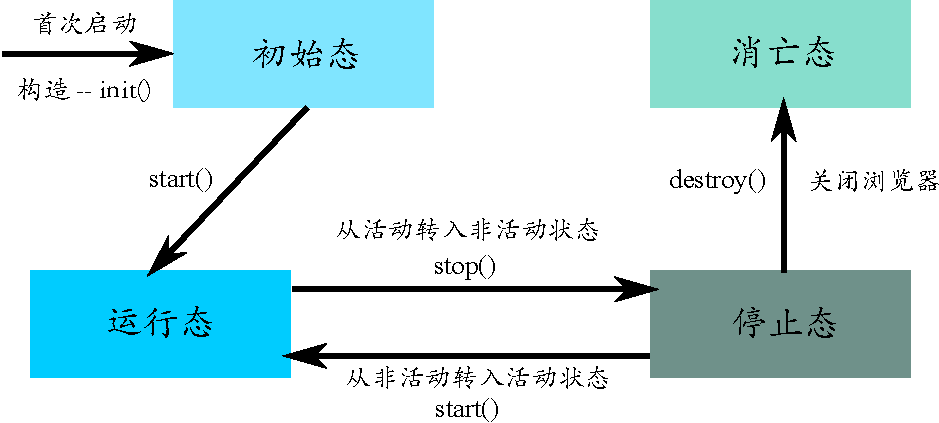
\includegraphics[width=0.8\textwidth]{figures/fig05.pdf}
  \end{figure}
\end{frame}


\begin{frame}[fragile] 
  \frametitle{Applet示例}

  \samp{GoodbyeApplet.java}
  
  \begin{javaCode}
    import java.applet.Applet;
    import java.awt.Color;
    import java.awt.Graphics;

    public class HelloApplet extends Applet {
      String text;
      public void init() {
        text = "Hello Applet, goodbye!";
        this.setBackground(new Color(120, 180, 140));
      }
      public void paint(Graphics g) {
        g.drawString(text, 25, 25);
      }
    }
  \end{javaCode}

  \samp{test.html}
  
  \begin{shCode}
    <html>
    <applet code="HelloApplet.class" width=200 height=150> </applet>
    </html>  
  \end{shCode}

  可以使用Applet viewer小工具运行示例:
  
  \begin{shCode}
    >appletviewer test.html
  \end{shCode}
\end{frame}

%%%%%%%%%%%%%%%%%%%%%%%%%%%%%%%%%%%%%%%%%%%%%%%%%%
\section{Swing概述}

\begin{frame}[fragile] % [fragile]参数使得能够插入代码
  \frametitle{Swing概述}

  \tta{Swing与AWT的关系}

  Swing是建立在AWT基础上的一种增强型Java GUI组件和工具集
  \begin{itemize}\kai
  \item 使用轻量组件以替代AWT中的绝大部分重量组件。
  \item 提供AWT所缺少的一些附件组件和观感控制机制。
  \item 提供更好的平台无关性。
  \end{itemize}

  \tta{相关基本概念}
  \ttc{Java基础类库(Java Foundation Classes, JFC)}\\
  Java基础类库是用于图形用户界面开发的Java API集,具体包括AWT、2D API、Swing组件
  和Accessibility API。
\end{frame}

\begin{frame}[fragile] % [fragile]参数使得能够插入代码
  \frametitle{Swing概述}
  \ttc{重量组件(Heavy-Weight Components)}\\
  \begin{itemize}
  \item 重量组件通过委托对等组件(对等组件指底层平台,如Windows操作系统的用户界面组件)来完
    成具体工作,包括组件的绘制和事件响应。AWT中的组件均为重量组件,或者说,AWT组件只是对本
    地对等组件的封装。
  \item 开销大、效率低、无法实现组件的“透明”效果。
  \end{itemize}
\end{frame}

\begin{frame}[fragile] % [fragile]参数使得能够插入代码
  \frametitle{Swing概述}

  \ttc{轻量组件(Light-Weight Components)}\\
  \begin{itemize}
  \item 轻量组件不存在本地对等组件,通过Java绘图技术在其所在的容器窗口中绘图得到。
  \item 能够实现组件的透明效果,能够做到不同平台上的一致表现。
  \item 组件绘制和事件处理机制的开销小。
  \item 轻量组件最终需要包含在一个重量容器中。因此,Swing组件中的几个顶层容器(如JFrame、
    JDialog和JApplet)采用了重量组件,其余的均为轻量组件。
  \item 不建议轻重组件混用。
  \end{itemize}
\end{frame}

\begin{frame}[fragile] % [fragile]参数使得能够插入代码
  \frametitle{Swing概述}
  \ttc{可视化组件(Visual Component)}

  \begin{itemize}
  \item 和AWT组件类似,Swing组件也分为可视化和非可视化组件。
  \item 可视化组件为能够显示特定形状、颜色和尺寸的组件;非可视化组件也称支持类,如布局管理
    器等。
  \item Swing可视化组件类名均以J开头。
  \end{itemize}
\end{frame}

\section{Swing典型组件(课后自学)}

\begin{frame}[fragile] % [fragile]参数使得能够插入代码
  \frametitle{JFrame}
  \begin{enumerate}
  \item JFrame继承并扩充了java.awt.Frame类。\\
    {\kai JFrame不再是一个单一容器,而是由相互间存在包含关系的多个不同容器面
      板(JRootPane, GlassPane, LayeredPane, ContentPane)组成,我们实际上只使用其中的内容
      面板(ContentPane)。}
  \item JFrame实现了javax.swing.WindowConstants接口,该接口中定义了用于控制窗口关闭操作的整型
    常量,包括:
    \begin{itemize}\small
    \item DO\_NOTHING\_ON\_CLOSE
    \item HIDE\_ON\_CLOSE
    \item DISPOSE\_ON\_CLOSE
    \item EXIT\_ON\_CLOSE
    \end{itemize}
  \end{enumerate}
\end{frame}

\begin{frame}[fragile] % [fragile]参数使得能够插入代码
  \frametitle{JFrame示例}
  \samp{TestJFrame.java}
  \begin{javaCode}
    import java.awt.Color;
    import java.awt.Container;
    import java.awt.FlowLayout;
    import javax.swing.JFrame;
    import javax.swing.JLabel;

    public class TestJFrame {
      public static void main(String[] args){
        JFrame jf = new JFrame("My Test");
        Container c = jf.getContentPane(); 
        c.setLayout(new FlowLayout(FlowLayout.LEFT, 20, 20));
        JLabel greet = new JLabel("Hello, World!");
        JLabel bye = new JLabel("Bye, World!");
        bye.setBackground(Color.BLUE);
        bye.setOpaque(true); // 设置为不透明
        c.add(greet);
        c.add(bye);
        c.setBackground(Color.GREEN);
        jf.setSize(400, 300);
        jf.setLocation(400, 200);
        jf.setDefaultCloseOperation(JFrame.EXIT_ON_CLOSE); // 等同于显示注册 WindowListener
        jf.setVisible(true);
      }
    }
  \end{javaCode}
\end{frame}

\begin{frame}[fragile] % [fragile]参数使得能够插入代码
  \frametitle{JFrame}

  为了方便开发,从JDK5.0开始JFrame类重写了其add()、remove()和setLayout()方法,这些重写后的方法{\hei 将针对JFrame的添加组件、移除组件和设置布局管理器等操作自动转发给其内容面板contentPane,以实现对contentPane的直接控制}。

  对上述代码的改写:

  \begin{javaCode}
    JFrame jf = new JFrame("My Test");
    jf.setLayout(new FlowLayout(FlowLayout.LEFT, 20, 20));
    JLabel greet = new JLabel("Hello, World!");
    jf.add(greet);
    jf.getContentPane().setBackground(Color.GREEN); // 注意
  \end{javaCode}

  {\Red\kai 注意:setBackground()方法在JFrame类中并没有进行重写,因此不会将针对JFrame的颜色设置操作自动转发到其内容面板。}
\end{frame}

\begin{frame}[fragile] % [fragile]参数使得能够插入代码
  \frametitle{Swing按钮、菜单和工具条}

  \begin{itemize}
  \item JButton\\
    能够实现更复杂的显式效果,例如可以使用图片作为按钮标签、设置快捷键和添加工具提示信息。
  \item 菜单\\
    同样分为菜单条、菜单和菜单项(JMenuBar、JMenu、JMenuItem),用法与AWT完全相同。
  \item 工具条\\
    工具条是用于显示常见组件的条形容器,一般用法是向工具条中添加一系列
    图标形式的按钮,并将之置于窗口上方边缘。{\kai 例如,BorderLayout布
      局的北部区域,对于大多数的外观,用户可以用鼠标直接将工具栏拖
      到BorderLayout布局的其他未添加组件的边缘区域,如西部或东部,也可
      以将之拖出到单独的窗口中显示。}
  \end{itemize}
\end{frame}

\begin{frame}[fragile] % [fragile]参数使得能够插入代码
  \frametitle{Swing按钮、菜单和工具条}

  \samp{TestSwing.java}

  \scriptsize
\begin{verbatim}
import java.awt.event.*;
import javax.swing.*;

public class TestSwing implements ActionListener {
  public static void main(String[] args) {
    new TestSwing().createUI();
  }

  public void createUI() {
    JFrame jf = new JFrame("Test Swing");
    JMenuBar jmb = new JMenuBar();
    JMenu menu_file = new JMenu("File");
    JMenu menu_help = new JMenu("Help");
    JMenuItem mi_new = new JMenuItem("New");
    JMenuItem mi_open = new JMenuItem("Open");
    JMenuItem mi_save = new JMenuItem("Save");
    mi_new.addActionListener(this);
    mi_open.addActionListener(this);
    mi_save.addActionListener(this);
\end{verbatim}
\end{frame}

\begin{frame}[fragile] % [fragile]参数使得能够插入代码
\frametitle{Swing按钮、菜单和工具条}
\scriptsize
\begin{verbatim}    
    mi_new.setMnemonic('N');
    mi_open.setMnemonic('O');
    mi_save.setMnemonic('S');
    menu_file.setMnemonic('F');
    menu_help.setMnemonic('h');
    
    menu_file.add(mi_new);
    menu_file.add(mi_open);
    menu_file.add(mi_save);
    
    jmb.add(menu_file);
    jmb.add(menu_help);

    JToolBar jtb = new JToolBar();
    JButton button_new = new JButton("NEW");
    JButton button_open = new JButton("OPEN");
    JButton button_save = new JButton("SAVE");

    button_new.setActionCommand("New");
    button_open.setActionCommand("Open");
    button_save.setActionCommand("Save");
\end{verbatim}
\end{frame}

\begin{frame}[fragile] % [fragile]参数使得能够插入代码
\frametitle{Swing按钮、菜单和工具条}
\scriptsize
\begin{verbatim}
    button_new.setToolTipText("Create a new file");
    button_open.setToolTipText("Open the file");
    button_save.setToolTipText("Save the file");
    
    button_new.addActionListener(this);
    button_open.addActionListener(this);
    button_save.addActionListener(this);
    
    jtb.add(button_new);
    jtb.add(button_open);
    jtb.add(button_save);
    
    JPanel jp = new JPanel();
    JButton button_start = new JButton("Start");
    JButton button_stop = new JButton("Stop");
    button_start.addActionListener(this);
    button_stop.addActionListener(this);
    jp.add(button_start);
    jp.add(button_stop);
\end{verbatim}
\end{frame}

\begin{frame}[fragile] % [fragile]参数使得能够插入代码
\frametitle{Swing按钮、菜单和工具条}
\scriptsize
\begin{verbatim}		
    jf.setJMenuBar(jmb); // Menu 不需要使用 add() 方法添加
    jf.add(jtb, "North");
    jf.add(jp, "South");
    
    jf.setSize(600, 400);
    jf.setLocation(400, 200);
    jf.setDefaultCloseOperation(JFrame.EXIT_ON_CLOSE);
    jf.setVisible(true);
  }

  @Override
  public void actionPerformed(ActionEvent e) {
    System.out.println(e.getActionCommand());
  }
}  
\end{verbatim}
\end{frame}

\begin{frame}[fragile] % [fragile]参数使得能够插入代码
\frametitle{标准对话框}

使用标准对话框(JOptionPane)可以实现程序与用户的便捷交互,如向用户发送错误通知、警告/确
认用户操作、接收用户输入或选择的简单信息等。

\samp{示例}
\scriptsize
\begin{verbatim}
  @Override
  public void actionPerformed(ActionEvent e) {
    String s = e.getActionCommand();
    if (s.equals("Error")) {
      JOptionPane.showMessageDialog(null, "这是一个错误提示对话框", "错误提示",
      JOptionPane.ERROR_MESSAGE);
    } else if (s.equals("Confirm Quit")) {
      int result = JOptionPane.showConfirmDialog(null, "真的要退出程序么?",
      "请确认退出", JOptionPane.YES_NO_OPTION);
      if (result == JOptionPane.OK_OPTION) {
        System.exit(0);
      }
\end{verbatim}
\end{frame}

\begin{frame}[fragile] % [fragile]参数使得能够插入代码
\frametitle{标准对话框}

\scriptsize
\begin{verbatim}
    } else if (s.equals("Warning")) {
      Object[] options = { "继续", "撤销" };
      int result = JOptionPane.showOptionDialog(null, "本操作可能导致数据丢失",
      "警告", JOptionPane.DEFAULT_OPTION,
      JOptionPane.WARNING_MESSAGE, null, options, options[0]);
      if (result == 0)
        System.out.println("继续操作");
    } else if (s.equals("Input")) {
      String name = JOptionPane.showInputDialog("请输入姓名:");
      if (name != null) 
        System.out.println("输入的姓名为" + name);
    } else if (s.equals("Choice")) {
      Object[] possibleValues = { "体育", "政治", "经济", "文化" };
      Object selectedValue = JOptionPane.showInputDialog(null,
      "Choice one", "Input", JOptionPane.INFORMATION_MESSAGE,
      null, possibleValues, possibleValues[0]);
      String result = (String) selectedValue;
      if (result != null) 
        System.out.println("你的选择是:" + result);
    }
  }
\end{verbatim}
\end{frame}

\begin{frame}[fragile] % [fragile]参数使得能够插入代码
\frametitle{表格和树}
\begin{itemize}
\item {\bf javax.swing.JTable}\\
用于以传统的表格形式来显示数据,通过注册监听器的方式关联响应的处理逻辑。
\begin{itemize}
\item 表头:标题行,给出每一列(字段)的名称。
\item 表体:由多行多列、规则矩阵形式的单元格组成,真正的数据信息则显示在每个单元格中。
\end{itemize}
\item {\bf javax.swing.JTree}\\
以树状结构分层次显示数据信息,例如操作系统提供的资源管理器。
\end{itemize}
\end{frame}

\begin{frame}[fragile] % [fragile]参数使得能够插入代码
\frametitle{表格示例}

\begin{columns}
\column{0.4\textwidth}  
\tta{表格}
\begin{figure}
\centering
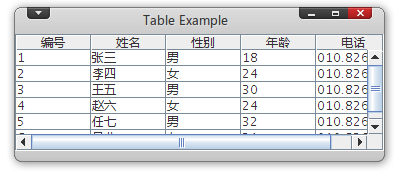
\includegraphics[width=0.95\textwidth]{swing-fig01.png}
\end{figure}

\column{0.6\textwidth}  
\begin{javaCode}
import java.awt.event.WindowAdapter;
import java.awt.event.WindowEvent;
import javax.swing.JFrame;
import javax.swing.JScrollPane;
import javax.swing.JTable;
public class TableExample {
  public static void main(String[] args) {
    JFrame myFrame = new JFrame("Table Example");
    Object data[][] = {
      {1, "张三", "男", "18", "010.82607080"},
      {2, "李四", "女", "24", "010.82607080"},
      {3, "王五", "男", "30", "010.82607080"},
      // ... ...
    };
    String columnNames[] = {
      "编号", "姓名", "性别", "年龄", "电话"};
    JTable table = new JTable(data, columnNames);
    table.setAutoResizeMode(JTable.AUTO_RESIZE_OFF);
    JScrollPane pane = new JScrollPane(table);
    myFrame.add("Center", pane);
    myFrame.setSize(450, 250);
    myFrame.addWindowListener(new WindowAdapter(){
      public void windowClosing(WindowEvent e) {
        System.exit(0);
      }
    });
    myFrame.setVisible(true);
  }
}
\end{javaCode}
\end{columns}
\end{frame}

\begin{frame}[fragile] % [fragile]参数使得能够插入代码
\frametitle{表格其他参考例程}
\begin{enumerate}
\item A Simple Interactive JTable Tutorial\\
http://www.javalobby.org/articles/jtable/
\end{enumerate}

\end{frame}
\begin{frame}[fragile] % [fragile]参数使得能够插入代码
\frametitle{树示例}

\tta{树}
\begin{figure}
\centering
\includegraphics[width=0.6\textwidth]{swing-fig02.png}
\end{figure}

\end{frame}

\begin{frame}[fragile] % [fragile]参数使得能够插入代码
\frametitle{树示例}

\samp{TreeExample.java}

\begin{javaCode}
public class TreeExample {
  public static DefaultMutableTreeNode createNodes() {
    DefaultMutableTreeNode rootNode = new DefaultMutableTreeNode("Java Stuff");
    DefaultMutableTreeNode resources = new DefaultMutableTreeNode("Resources");
    DefaultMutableTreeNode tools = new DefaultMutableTreeNode("Tools");
    rootNode.add(resources);
    rootNode.add(tools);
    DefaultMutableTreeNode webSites = new DefaultMutableTreeNode("Web Sites");
    DefaultMutableTreeNode books = new DefaultMutableTreeNode("Books");
    resources.add(webSites);
    resources.add(books);
    tools.add(new DefaultMutableTreeNode("JBuilder"));
    tools.add(new DefaultMutableTreeNode("Visual J++"));
    return rootNode;
  }
  public static void main(String[] args) {
    JFrame myFrame = new JFrame("Tree Example");
    DefaultMutableTreeNode rootNode = createNodes();
    JTree tree = new JTree(rootNode);
    tree.setRootVisible(true);
    JScrollPane pane = new JScrollPane();
    pane.setViewportView(tree);
    myFrame.add(pane, "Center");
    myFrame.setSize(400, 250);
    myFrame.setDefaultCloseOperation(JFrame.EXIT_ON_CLOSE);
    myFrame.setVisible(true);
  }
}
\end{javaCode}
\end{frame}

\begin{frame}[fragile] % [fragile]参数使得能够插入代码
\frametitle{JTable和JTree的MVC模式}

JTable和JTree采用了相对独立的方式向组件提供要显示的数据,即当显示/处理的数据结构较复杂
时,将GUI组件结构分为相对独立的{\hei 模型、视图、控制器}三个模块,模块间存在专门的分工和
协作关系。
\begin{enumerate}\kai 
\item {\hei 模型(Model)} 维护数据并提供数据访问方法,即数据和数据的处理逻辑。
\item {\hei 视图(View)} 绘制模型的视觉表现,即显示数据。视图就是用户能够看到并与之进行
  交互的用户界面。
\item {\hei 控制器(Controllor)} 负责处理事件或者说程序的流程控制,接受用户输入,并调
  用/操控模型和视图以实现用户需求。
\end{enumerate}
\end{frame}

\begin{frame}[fragile] % [fragile]参数使得能够插入代码
\frametitle{MVC作用原理}

\begin{figure}
\centering
\includegraphics[width=0.5\textwidth]{swing-fig02.pdf}
\end{figure}
\end{frame}

\begin{frame}[fragile] % [fragile]参数使得能够插入代码
\frametitle{定时器}

javax.swing.Timer提供了定时器功能,用于在指定的时间延迟之后触发ActionEvent事件,以执行所
需的处理逻辑。

{\kai 具体的做法是:首先创建Timer对象,并在其上注册一个或多
  个ActionListener类型的监听器,在监听器事件处理方法actionPerformed()中
  应以实现给出要延时执行的任务代码,然后调用Timer对象的start()方法启动
  定时器即可。}

\tta{相关方法} 
\begin{itemize}
\item setRepeats() 设置计时器的动作。
\item setInitialDelay() 设置首次延迟时间。
\item start() 开始计时器。
\item stop() 停止计时器。
\item restart() 恢复计时器。
\end{itemize}
\end{frame}

\begin{frame}
  \frametitle{本节习题}
  \begin{enumerate}
  \item 制作思维导图,梳理Java Swing GUI库中各组件功能及编程知识点,看
    看谁总结的好,做的漂亮。
  \item 自行了解Java FX,参考互联网公开资料写一个Sample Code出来。
  \end{enumerate}
\end{frame}
%%%%%%%%%%%%%%%%%%%%%%%%%%%%%%%%%%%%%%%%%%%%%%%%%%%%%%%%%%%%%%%%%%%%%%%%%%%%%%%
% TKS Page %%%%%%%%%%%%%%%%%%%%%%%%%%%%%%%%%%%%%%%%%%%%
\begin{frame}
\centering
{\Huge \textcolor{blue}{THE END}} \\
\vspace{5mm}
{\Large wangxiaodong@ouc.edu.cn} \\
\end{frame}
%%%%%%%%%%%%%%%%%%%%%%%%%%%%%%%%%%%%%%%%%%%%%%%%%%%%%%%
%%%%%%%%%%%%%%%%%%%%%%%%%%%%%%%%%%%%%%%%%%%%%%%%%%%%%%%%%%%%%%%%%%%%%%%%%%%%%%%
\end{document}



% Week 07 %%
\chapter{异常处理}
\label{chp:Java-exception-handling}

\section*{基本信息}
\sline
\begin{description}
\item[课程名称:] Java应用与开发
\item[授课教师:] 王晓东
\item[授课时间:] 第七周
\item[参考教材:] 本课程参考教材及资料如下:
  \begin{itemize}
  \item 陈国君主编,Java程序设计基础(第5版),清华大学出版社,2015.5
  \item Bruce Eckel, Thinking in Java (3rd)
  \end{itemize}
\end{description}

\section*{教学目标}

\sline

\begin{enumerate}
\item 掌握Java异常的概念和分类
\item 深入理解Java异常处理机制
\end{enumerate}  

\section*{授课方式}

\sline
\begin{description}
\item[理论课:] 多媒体教学、程序演示
\item[实验课:] 上机编程
\end{description}

\newpage
\section*{教学内容}
\sline

%%%%%%%%%%%%%%%%%%%%%%%%%%%%%%%%%%%%%%%%%%%%%%%%%%%%%%%%%%%%%%
\section{异常的概念及分类}

\subsection{什么是异常}

在Java语言中,程序运行出错被称为出现异常。异常(Exception)是程序运行过
程中发生的事件,该事件可以中断程序指令的正常执行流程。Java异常分为两大类:

\begin{description}
\item[错误(Error)] 是指JVM系统内部错误、资源耗尽等严重情况。
\item[违例(Exception)] 则是指其他因编程错误或偶然的外在因素导致的一般
  性问题,例如对负数开平方根、空指针访问、试图读取不存在的文件以及网络
  连接中断等。
\end{description}

给出一个Java运行时异常的示例:

\samplecode{TestException.java}

\begin{javaCode}
public class TestException {
  public static void main(String[] args) {
    String friends[] = {"Lisa", "Bily", "Kessy"};
    for(int i = 0; i < 5; i++) {
      System.out.println(friends[i]);
    }
    System.out.println("\n this is the end");
  }
}
\end{javaCode}

标准输出如下,程序编译通过,但运行时出错。

\begin{stdoutCode}
Lisa
Bily
Kessy
Exception in thread "main" java.lang.
ArrayIndexOutOfBoundsException: 3
at TestException.main(TestException.java:6)
\end{stdoutCode}

\subsection{Java异常分类}
 
Throwable类是Java语言中所有异常类的父类。Java异常分类如
图\ref{fig:exception-class}所示。

\begin{figure}[h]
\centering
\includegraphics[width=0.95\textwidth]{images/Java-exception-handling/fig-exception-class.png}
\caption{Java异常分类}
\label{fig:exception-class}
\end{figure}

\subsection{常见错误}

\subsubsection{链接错误(LinkageError)}

LinkageError是指程序链接错误。例如,一个类中用到另外一个类,在编译前一
个类之后,后一个类发生了不相容的改变时,再使用前一个类则会出现链接错误。
最常见的就是后一个类的.class文件被误删除。

\subsubsection{虚拟机错误(VirtualMachineError)}
 
当Java虚拟机崩溃或用尽了它继续操作所需的资源时,会抛出该错误。其中比较
有代表性的是StackOverflowError,当应用程序递归太深而导致栈内存溢出时会
出现该异常。

\samplecode{TestVMerror.java}

\begin{javaCode}
  public class TestVMError {
    public static void main(String[] args) {
      TestVMError t = new TestVMError();
      t.f(100000);
    }
    public int f(int n) {
      if (n <= 0) {
        return 0;
      }
      int k = n * this.f(n-1);
      return k;
    }
  }
\end{javaCode}

标准输出如下:

\begin{stdoutCode}
  Exception in thread "main" java.lang.StackOverflowError
  at TestException.f(TestException.java:7)
  at TestException.f(TestException.java:10)  
\end{stdoutCode}

\subsection{常见异常}

\subsubsection{运行时异常(RuntimeException)}

运行时异常主要包括:

\begin{itemize}
\item 错误的类型转换;
\item 数组下标越;
\item 空指针访问。
\end{itemize}

其中,空指针异常(NullPointerException)是如果试图访问不指向任何对象的
引用变量的成员,将会产生空指针异常。例如:

\begin{javaCode}
Person p = null;
System.out.println(p.age);  
\end{javaCode}

\subsubsection{IO异常(IOException)}

\begin{itemize}
\item 从一个不存在的文件中读取数据;
\item 越过文件结尾继续读取;
\item 连接一个不存在的URL。
\end{itemize}

以下给出IOException的一个示例,注意下述代码无法通过编译!

\samplecode{TestIOException.java}

\begin{javaCode}
import java.io.*;
public class TestIOException {
  public static void main(String[] args) {
    FileInputStream in = new FileInputStream("myfile.txt");
    int b;
    b = in.read();
    while (b != -1) {
      System.out.print((char) b);
      b = in.read();
    }
    in.close();
  }
}  
\end{javaCode}

\notice{对上述代码无法编译的解释}

只要是有可能出现IOException的Java代码,在编译时就会出错,而不会等到运行
时才发生。编译出错信息大致如下:

\begin{stdoutCode}
TestIOException.java:4: 未报告的异常 java.io.FileNotFoundException; 
必须对其进行捕捉或声明以便抛出
    FileInputStream in = new FileInputStream("myfile.txt");
... ...
\end{stdoutCode}

\section{Java异常处理机制}

Java异常处理的宗旨包括:

\begin{itemize}
\item 返回到一个安全和已知的状态;
\item 能够使用户执行其他的命令;
\item 如果可能,则保存所有的工作;
\item 如果有必要,可以退出以避免造成进一步的危害。
\end{itemize}

Java异常处理的基本机制是:

\begin{itemize}
\item Java程序执行过程中如出现异常,系统会监测到并自动生成一个相应的异常类对象,然后再将它
  交给运行时系统;
\item 运行时系统再寻找相应的代码来处理这一异常。如果Java运行时系统找不到可以处理异常的代
  码,则运行时系统将终止,相应的Java程序也将退出。
\item 程序本身通常对错误(Error)无能为力,因而一般只处理违例(Exception)。
\end{itemize}

\subsection{捕获异常}

Java语言捕获异常的基本程序逻辑结构如下:

\begin{javaCode}
try {
  ... //可能产生异常的代码
} catch (ExceptionName1 e) {
  ... //当产生 ExceptionName1 型异常时的处置措施
} catch (ExceptionName2 e) {
  ... //当产生 ExceptionName2 型异常时的处置措施
} finally {
  ... //无条件执行的语句
}
\end{javaCode}

以下给出一段捕获处理数组访问越界异常的示例:

\samplecode{ArrayIndexOutOfBoundsExceptionSample.java}

\begin{javaCode}
public class ArrayIndexOutOfBoundsExceptionSample {
  public static void main(String[] args) {
    String friends[]={"Lisa","Billy","Kessy"};
    try {
      for(int i = 0; i < 5; i++) {
        System.out.println(friends[i]);
      }
    } catch(ArrayIndexOutOfBoundsException e) {
      System.out.println("index err");
    }
    System.out.println("\nthis is the end");
  }
}
\end{javaCode}

\subsection{使用finally语句}

Java异常处理中,finally语句是可选的,其作用是为异常处理提供一个统一的出口,使得在控制流转到程序的其他部分以前,能够对程序的状态作统一的管理。

\samplecode{FinallySample.java}

\begin{javaCode}
public class FinallySample {
  public static void main(String[] args) {
    String friends[]={"Lisa","Billy","Kessy"};
    try {
      for (int i = 0; i < 5; i++) {
        System.out.println(friends[i]);
      }
    } catch(ArrayIndexOutOfBoundsException e) {
      System.out.println("index err");
      return;
    } finally {
      System.out.println("in finally block!");
    }
    System.out.println("this is the end");
  }
}
  
\end{javaCode}

注意,不论try代码块中是否发生了异常事件,finally块中的语句都会被执行。当catch语句块中出现return
语句时,finally语句块同样会执行。上述代码的输出:

\begin{stdoutCode}
Lisa
Billy
Kessy
index err
in finally block!  
\end{stdoutCode}

\subsection{操纵异常对象}

发生异常时,系统将自动创建异常类对象,并将作为实参传递给匹配的catch语句块的形参,这样我们
就可以在语句块中操纵该异常对象了。主要使用异常类的父类Throwable中定义的两个成员方法:

\begin{itemize}
\item public String getMessage() 返回描述当前异常的详细消息字符串;
\item public void printStackTrace() 用来跟踪异常事件发生时运行栈的内容,并将相关信息输出
  到标准错误输出设备。本方法比较常用,在没有找到适合的异常处理代码时,系统也会自动调用该
  方法输出错误信息。
\end{itemize}

可以参考以下代码追踪运行栈信息:

\samplecode{A.java}

\begin{javaCode}
public class A {
  public void work(int[] a) {
    String s = this.contain(a, 3);
    System.out.println("Result: " + s);
  }

  public String contain(int[] source, int dest) {
    String result = "no!";
    try {
      for (int i = 0; i < source.length; i++) {
        if (source[i] == dest)
        result = "yes!";
      }
    } catch(Exception e) {
      System.out.println("异常信息:" + e.getMessage());
      System.out.println("运行栈信息:");
      e.printStackTrace();
      result = "error!";
    }
    return result;
  }
}
\end{javaCode}

\samplecode{MyTest.java}

\begin{javaCode}
public class MyTest {
  public static void main(String[] args) {
    A tst = new A();
    tst.work(null);
  }
}
\end{javaCode}

程序输出结果如下:

\begin{stdoutCode}
Exception Message: null
Stack Trace:
java.lang.NullPointerException
    at A.contain(A.java:9)
    at A.work(A.java:3)
    at MyTest.main(MyTest.java:4)
Result: error!
\end{stdoutCode}

\subsection{捕获和处理IOException}

以下给出捕获和处理IOException的示例:

\samplecode{TestIOException.java}

\begin{javaCode}
import java.io.*;
public class TestIOException {
  public static void main(String[] args) {
    try {
      FileInputStream in = new FileInputStream("myfile.txt");
      int b;
      b = in.read();
      while(b != -1) {
        System.out.print((char) b);
        b = in.read();
      }
      in.close();
    } catch (FileNotFoundException e) {
      System.out.println("File is missing!");
    } catch (IOException e) {
      e.printStackTrace();
    }
    System.out.println("It's ok!");
  }
}
\end{javaCode}

FileNotFoundException是IOException的子类,基于多态性机制,后一个catch语
句也可以处理FileNotFoundException,因此前一个catch语句块可以取消,但这
样就无法区分是“文件不存在”引发异常或其他I/O异常了。

\notice{异常处理知识点}

\begin{enumerate}
\item 对于只可能产生RuntimeException的代码可以不使用try-catch语句进行处
  理,如果对于这些相对安全的代码仍然采用了try语句块的形式,则try后可以
  省略catch语句块或finally语句块,但不能同时省略。
\item 如果试图捕获和处理代码中根本不可能出现的异常,编译器也会指出这种
  不当行为。
\end{enumerate}

\subsection{声明抛出异常}
 
声明抛弃异常是Java中处理违例的第二种方式如果。一个方法中的代码在运行时
可能生成某种异常,但在本方法中不必、或者不能确定如何处理此类异常时,则
可以声明抛弃该异常;此时方法中将不对此类异常进行处理,而是由该方法的调用
者负责处理。 语法格式如下:

\begin{javaCode}
  [< 修饰符 >] < 返回值类型 > < 方法名 > (< 参数列表 >) [throws < 异常类型 > [,< 异常类型 >]*] {
    [< Java语句 >]*
  }
\end{javaCode}

\samplecode{TestThrowsException.java}

\begin{javaCode}
import java.io.*;
public class TestThrowsException {
  public static void main(String[] args) {
    TestThrowsException t = new TestThrowsException();
    try {
      t.readFile();
    } catch (IOException e) {
      System.out.println(e);
    }
  }
  public void readFile() throws IOException {
    FileInputStream in = new FileInputStream("myfile.txt");
    int b;
    b = in.read();
    while (b != -1) {
      System.out.print((char) b);
      b = in.read();
    }
    in.close();
  }
}
\end{javaCode}
 
\notice{声明抛出异常的注意事项}

\begin{enumerate}
\item 除非事先约定,否则在开发过程中不要在自己编写的方法中采用抛出异常
  的方式。
\item 重写方法不允许抛出比被重写方法范围更大的异常类型。例
  如 IOException重写后抛出FileNotFoundException和EOFException被允许,而
  抛出Exception则不被允许。
\end{enumerate}
 
\subsection{人工抛出异常}

Java异常类对象除了在程序运行出错时由系统自动生成并抛出之外,也可根据需
要人工创建并抛出:

\begin{javaCode}
IOException e = new IOException(); // 创建异常类对象
throw e; // 抛出操作,即将该异常对象提交给Java运行环境
\end{javaCode}

被抛出的必须是Throwable或其子类类型的对象。例如,下述语句因为人工抛出的
并非Throwable或其子类的对象,在编译时会产生语法错误:

\begin{javaCode}
throw new String("want to throw");  
\end{javaCode}

以下给出一个人工抛出异常的示例:

\samplecode{TextThrowException.java}

\begin{javaCode}
import java.util.Scanner;

public class TestThrowException {
  public static void main(String[] args) {
    TestThrowException t = new TestThrowException();
    System.out.print("Please input your age: ");
    System.out.print("Your age: " + t.inputAge());
  }
  public int inputAge() {
    int result = -1;
    Scanner scan = new Scanner(System.in);
    while (true) {
      try {
        result = scan.nextInt();
        if (result < 0 || result > 130) {
          Exception me = new Exception("You come from Mars? ");
          throw me;
        }
        break;
      } catch (Exception e1) {
        System.out.println(e1.getMessage() + "Please input your age again: ");
        continue;
      }
    }
    return result;
  }
}
\end{javaCode}

上述代码所述的情况利用异常处理机制实现数据取值范围的检查并不太合适。应
用异常处理机制的原则如下:

\begin{itemize}
\item 当明确知道可能出错的地方或能够通过简单的检查而有效防止错误发生,
  就应该使用if-else语句来预防错误发生;
\item 只有当我们无法明确知道错误发生之处或无法完全避免异常,才不得不通
  过异常处理的方式来捕获和处理异常。
\end{itemize}


\section{用户自定义异常}

Java语言及许多类库针对常见异常状况已事先定义了相应的异常类型,并在程序
运行出错时由系统自动创建相应异常对象并进行抛出、捕获和处理,因此一般不
需要用户人工抛出异常对象或定义新的异常类型,但针对特殊的需要也可以这样
做。

我们一般通过继承Exception类来实现异常类型自定义,由于用户自定义的异常不
会由系统自动检测并抛出,所以只能靠人工触发并抛出。

以下给出用户自定义异常的示例:

\samplecode{CustomizingException.java}

\begin{javaCode}
public class CustomizingException extends Exception {
  private int idnumber;

  public MyException(String message, int id) {
    super(message);
    this.idnumber = id;
  }

  public int getId() {
    return idnumber;
  }
}
\end{javaCode} 

上述自定义异常类代码的构造方法中使用super调用其父类Exception的有参构造
方法,以便在创建异常对象时将用户的定制的报错信息传递给父类中定义
的private属性Message(该属性由Throwable类定义),将来在捕获和处理异常时
就可以通过调用该对象的getMessage()方法访问到该信息。

\samplecode{TestCustomizingException.java}

\begin{javaCode}
public class TestCustomizingException {
  public void regist(int num) throws MyException {
    if (num < 0) {
      throw new MyException("人数为负值,不合理", 3);
    }
    System.out.println("登记人数:" + num);
  }

  public void manager() {
    try {
      regist(-100);
    } catch (MyException e) {
      System.out.println("登记失败,出错种类" + e.getId());
      e.printStackTrace();
    }
    System.out.print("本次登记操作结束");
  }

  public static void main(String args[]) {
    new TestCustomizingException().manager();
  }
}
\end{javaCode}

上述测试程序输出结果如下:

\begin{stdoutCode}
登记失败,出错种类3
MyException: 人数为负值,不合理 ...
\end{stdoutCode}

\section{断言}

\subsection{什么是断言}

从JDK1.4版本开始,Java语言中引入了断言(Assert)机制,允许Java开发者在
代码中加入一些检查语句,主要目的是用于程序调试。

\begin{itemize}
\item 当我们需要在约定的条件不成立时中断当前程序执行操作的话可以使用断言;
\item 使用断言是为了在测试阶段确定程序内部出错位置和出错信息,而不是控制程序流程;
\item 断言机制在用户定义的boolean表达式(判定条件)结果为false时抛出一
  个Error对象,其类型为AssertionError;
\item 作为Error的一种,断言失败也不需捕获处理或者声明抛出,一旦出现了则
  终止程序、不必进行补救和恢复。

\end{itemize}

\subsection{启用和禁用断言}

\subsubsection{命令行开启断言功能}

Java运行时环境默认设置为关闭断言功能,因此在使用断言以前,需要在运
行Java程序时先开启断言功能。方法如下:

\begin{shCode}
>java -ea MyAppClass
\end{shCode}

或者:

\begin{shCode}
>java -enableassertions MyAppClass  
\end{shCode}

\subsubsection{命令行关闭断言功能}

\begin{shCode}
>java -da MyAppClass  
\end{shCode}

或者:

\begin{shCode}
java -disableassertions MyAppClass  
\end{shCode}

\subsubsection{Eclipse IDE开启断言}

在项目上点击右键 \ding{224} Run As \ding{224} Run Configurations \ding{224} Arguments,
在VM arguments中,加入-enableassertions或-ea即可。

\subsection{使用断言}

第一种断言的语法格式如下:

\begin{javaCode}
assert <boolean 表达式>;  
\end{javaCode}

以下给出使用第一种断言语法的示例代码:

\samplecode{TestAssertion.java}

\begin{javaCode}
public class TestAssertion {
  public static void main(String[] args) {
    new TestAssertion().process(-12);
  }
  public void process(int age) {
    assert age >= 0;
    System.out.println("您的年龄:" + age);
    // ---
  }
}
\end{javaCode}

以上程序执行的输出如下:

\begin{stdoutCode}
Exception in thread "main" java.lang.AssertionError
	at TestAssertion.process(TestAssertion.java:8)
	at TestAssertion.main(TestAssertion.java:4)  
\end{stdoutCode}

第二种断言的语法格式如下:

\begin{javaCode}
assert < boolean 表达式 >:< 表达式 2 >;  
\end{javaCode}

以下给出第二种断言格式的示例代码:

\samplecode{TestAssertion2.java}

\begin{javaCode}
public class TestAssertion2 {
  public static void main(String[] args) {
    new TestAssertion2().process(-12);
  }
  public void process(int age) {
    assert age >= 0: "年龄值不合理";
    System.out.println("您的年龄:" + age);
    //---
  }
}
\end{javaCode}

输出结果如下:

\begin{stdoutCode}
Exception in thread "main" java.lang.AssertionError: 年龄值不合理
	at TestAssertion.process(TestAssertion.java:8)
	at TestAssertion.main(TestAssertion.java:4)  
\end{stdoutCode}

\descript{说明}

断言失败时,系统会自动将表达式2的值传递给新创建的AssertionError对象,进
而将其转换为一个消息字符串保存起来,这样就可以在获得更多/更有针对性的检
查失败细节信息。因此,其中的表达式2可以是任何基本数据类型或引用数据类型,
但必须提供一个值,即不能为空值。

\section{课后习题}

\begin{enumerate}
\item 总结Java的异常处理机制。
\item 什么是运行时异常?
\item 若try语句结构中有多个catch()子句,这些子句的排列顺序与程序执行效果是否有关?
\item 总结Java异常处理机制随Java版本的更新不断加入的新特性,并附参考文献或网站链接。(选做)
\end{enumerate}
%%%%%%%%%%%%%%%%%%%%%%%%%%%%%%%%%%%%%%%%%%%%%%%%%%%%%%%%%%%%%%%%%%%%%%%%%%%%%%%
\documentclass[hyperref={pdfpagelabels=false},compress,table]{beamer} % 在Mac下无法编译
% \documentclass[compress,table]{beamer} % 在Mac下使用
% package for font
\usepackage{fontspec}
\defaultfontfeatures{Mapping=tex-text}  %%如果没有它,会有一些 tex 特殊字符无法正常使用,比如连字符。
\usepackage{xunicode,xltxtra}
\usepackage[BoldFont,SlantFont,CJKnumber,CJKchecksingle]{xeCJK}  % \CJKnumber{12345}: 一万二千三百四十五
\usepackage{CJKfntef}  %%实现对汉字加点、下划线等。
\usepackage{pifont}  % \ding{}
% package for math
\usepackage{amsfonts}

% package for graphics
\usepackage[americaninductors,europeanresistors]{circuitikz}
\usepackage{tikz}
\usetikzlibrary{plotmarks}  % placements=positioning
\usepackage{graphicx}  % \includegraphics[]{}
\usepackage{subfigure}  %%图形或表格并排排列
% package for table
\usepackage{colortbl,dcolumn}  %% 彩色表格
\usepackage{multirow}
\usepackage{multicol}
\usepackage{booktabs}
% package for code
\usepackage{fancyvrb}
\usepackage{listings}

% \usepackage{animate}
% \usepackage{movie15}

%%%%%
% setting for beamer
\usetheme{default} % Madrid(常用), Copenhagen, AnnArbor, boxes(白色), Frankfurt,Berkeley
\useoutertheme[subsection=true]{miniframes} % 使用Berkeley时注释本行
\usecolortheme{sidebartab}
\usefonttheme{serif}  %%英文使用衬线字体
% \setbeamertemplate{background canvas}[vertical
% shading][bottom=white,top=structure.fg!7] %%背景色,上25%的蓝,过渡到下白。
\setbeamertemplate{theorems}[numbered]
\setbeamertemplate{navigation symbols}{}  %% 去掉页面下方默认的导航条
\setbeamercovered{transparent}  %设置 beamer 覆盖效果

% 设置标题title背景色
% \setbeamercolor{title}{fg=black, bg=lightgray!60!white}
\setbeamercolor{title}{fg=white, bg=black!70!white}

% 设置每页小LOGO
\pgfdeclareimage[width=1cm]{ouc}{figures/static/ouc.pdf}
\logo{\pgfuseimage{ouc}{\vspace{-20pt}}}

% setting for font
%%\setCJKmainfont{Adobe Kaiti Std}
\setCJKmainfont{SimSun} 
%% \setCJKmainfont{FangSong_GB2312} 
%% \setmainfont{Apple Garamond}  %%苹果字体没有SmallCaps
\setCJKmainfont{SimSun} 
%FUNNY%\setCJKmainfont{DFPShaoNvW5-GB}  %%华康少女文字W5(P)
%FUNNY%\setCJKmainfont{FZJingLeiS-R-GB}  %%方正静蕾体
%FUNNY%\setmainfont{Purisa}
%\setsansfont[Mapping=tex-text]{Adobe Song Std}
     %如果装了Adobe Acrobat,可在font.conf中配置Adobe字体的路径以使用其中文字体。
     %也可直接使用系统中的中文字体如SimSun、SimHei、微软雅黑等。
     %原来beamer用的字体是sans family;注意Mapping的大小写,不能写错。
     %设置字体时也可以直接用字体名,以下三种方式等同:
     %\setromanfont[BoldFont={黑体}]{宋体}
     %\setromanfont[BoldFont={SimHei}]{SimSun}
     %\setromanfont[BoldFont={"[simhei.ttf]"}]{"[simsun.ttc]"}
% setting for graphics
\graphicspath{{figures/}}  %%图片路径
\renewcommand\figurename{图}

% setting for pdf
\hypersetup{% pdfpagemode=FullScreen,%
            pdfauthor={Xiaodong Wang},%
            pdftitle={Title},%
            CJKbookmarks=true,%
            bookmarksnumbered=true,%
            bookmarksopen=false,%
            plainpages=false,%
            colorlinks=true,%
            citecolor=green,%
            filecolor=magenta,%
            linkcolor=blue,%red(default)
            urlcolor=cyan}

% setting for fontspec
\XeTeXlinebreaklocale "zh"  %%表示用中文的断行
\XeTeXlinebreakskip = 0pt plus 1pt minus 0.1pt  %%多一点调整的空间
%%%%%

% font setting by xeCJK
\setCJKfamilyfont{NSimSun}{NSimSun}
\newcommand{\song}{\CJKfamily{NSimSun}}
%%%\setCJKfamilyfont{AdobeSongStd}{Adobe Song Std}
%%%\newcommand{\AdobeSong}{\CJKfamily{AdobeSongStd}}
\setCJKfamilyfont{FangSong}{FangSong_GB2312}
\newcommand{\fang}{\CJKfamily{FangSong}}
%%%\setCJKfamilyfont{AdobeFangsongStd}{Adobe Fangsong Std}
%%%\newcommand{\AdobeFang}{\CJKfamily{AdobeFangsongStd}}
\setCJKfamilyfont{SimHei}{SimHei}
\newcommand{\hei}{\CJKfamily{SimHei}}
%%%\setCJKfamilyfont{AdobeHeitiStd}{Adobe Heiti Std}
%%%\newcommand{\AdobeHei}{\CJKfamily{AdobeHeitiStd}}
\setCJKfamilyfont{KaiTi}{KaiTi}
\newcommand{\kai}{\CJKfamily{KaiTi}}
%%%\setCJKfamilyfont{AdobeKaitiStd}{Adobe Kaiti Std}
\newcommand{\AdobeKai}{\CJKfamily{AdobeKaitiStd}}
\setCJKfamilyfont{LiSu}{LiSu}
\newcommand{\li}{\CJKfamily{LiSu}}
\setCJKfamilyfont{YouYuan}{YouYuan}
\newcommand{\you}{\CJKfamily{YouYuan}}
\setCJKfamilyfont{FZJingLei}{FZJingLeiS-R-GB}
\newcommand{\jinglei}{\CJKfamily{FZJingLei}}
\setCJKfamilyfont{MSYH}{Microsoft YaHei}
\newcommand{\msyh}{\CJKfamily{MSYH}}

% 自定义颜色
\def\Red{\color{red}}
\def\Green{\color{green}}
\def\Blue{\color{blue}}
\def\Mage{\color{magenta}}
\def\Cyan{\color{cyan}}
\def\Brown{\color{brown}}
\def\White{\color{white}}
\def\Black{\color{black}}

\lstnewenvironment{xmlCode}[1][]{% for Java
  \lstset{
    basicstyle=\tiny\ttfamily,%
    columns=flexible,%
    framexleftmargin=.7mm, %
    % frame=shadowbox,%
    % rulesepcolor=\color{cyan},%
     frame=single,%
    backgroundcolor=\color{white},%
    xleftmargin=4\fboxsep,%
    xrightmargin=4\fboxsep,%
    numbers=left,numberstyle=\tiny,%
    numberblanklines=false,numbersep=7pt,%
    language=xml, %
    }\lstset{#1}}{}

\lstnewenvironment{javaCode}[1][]{% for Java
  \lstset{
    basicstyle=\tiny\ttfamily,%
    columns=flexible,%
    framexleftmargin=.7mm, %
    frame=shadowbox,%
    rulesepcolor=\color{cyan},%
    % frame=single,%
    backgroundcolor=\color{white},%
    xleftmargin=4\fboxsep,%
    xrightmargin=4\fboxsep,%
    numbers=left,numberstyle=\tiny,%
    numberblanklines=false,numbersep=7pt,%
    language=Java, %
    }\lstset{#1}}{}

\lstnewenvironment{shCode}[1][]{% for Java
  \lstset{
    basicstyle=\scriptsize\ttfamily,%
    columns=flexible,%
    framexleftmargin=.7mm, %
    frame=shadowbox,%
    rulesepcolor=\color{brown},%
    % frame=single,%
    backgroundcolor=\color{white},%
    xleftmargin=4\fboxsep,%
    xrightmargin=4\fboxsep,%
    numbers=left,numberstyle=\tiny,%
    numberblanklines=false,numbersep=7pt,%
    language=sh, %
    }\lstset{#1}}{}

\newcommand\ask[1]{\vskip 4bp \tikz \node[rectangle,rounded corners,minimum size=6mm,
  fill=white,]{\Cyan \includegraphics[height=1.5cm]{question} \Large \msyh #1};}

\newcommand\wxd[1]{\vskip 4bp \tikz \node[rectangle,minimum size=6mm,
  fill=blue!60!white,]{\White \ding{118} \msyh #1};}

\newcommand\xyy[1]{\vskip 2bp \tikz \node[rectangle,minimum size=3mm,
  fill=black!80!white,]{\White \msyh\scriptsize #1};}

\newcommand\cxf[1]{\vskip 4bp \tikz \node[rectangle,rounded corners,minimum size=6mm,
  fill=orange!60!white,]{\White \ding{42} \msyh #1};}

\newcommand\samp[1]{\vskip 2bp \tikz \node[rectangle,minimum size=3mm,
  fill=white!100!white,]{\Mage\msyh \small CODE \ding{231} \Black #1};\vskip -8bp}

\newcommand\zhyfly[1]{\tikz \node[rectangle,rounded corners,minimum size=6mm,ball color=red!25!blue,text=white,]{#1};}

\setbeamerfont{frametitle}{series=\msyh} % 修改Beamer标题字体

\makeatletter
\newcommand{\Extend}[5]{\ext@arrow 0099{\arrowfill@#1#2#3}{#4}{#5}}
\makeatother


%%%%%%%%%%%%%%%%%%%%%%%%%%%%%%%%%%%%%%%%%%%%%%%%%%%%%%%%%%%%%%%%%%%%%%%%%%%%%%%
% \titlepage
\title[KevinW@OUC]{\hei {\huge Java 应用与开发}\\  
  高级I/O编程}
\author[王晓东]{王晓东\\
  \href{mailto:wangxiaodong@ouc.edu.cn}{\footnotesize wangxiaodong@ouc.edu.cn}}
\institute[中国海洋大学]{\small 中国海洋大学}
\date{\today}
\titlegraphic{\vspace{-6em}\includegraphics[height=6cm]{static/ouc.pdf}\vspace{-6em}}
%%%%%
\begin{document}
%% Delete this, if you do not want the table of contents to pop up at
%% the beginning of each subsection:
\AtBeginSection[]{                              % 在每个Section前都会加入的Frame
  \frame<handout:0>{
    \frametitle{\textbf{\hei 接下来…}}
    \tableofcontents[currentsection]
  }
}  %

\AtBeginSubsection[]                            % 在每个子段落之前
{
  \frame<handout:0>                             % handout:0 表示只在手稿中出现
  {
    \frametitle{\textit{\hei 接下来…}}\small
    \tableofcontents[current,currentsubsection] % 显示在目录中加亮的当前章节
  }
}
\frame{\titlepage}
%%%%%%%%%%%%%%%%%%%%%%%%%%%%%%%%%%%%%%%%%%%%%%%%%%%%%%%%%%%%%%%%%%%%%%%%%%%%%%%
\begin{frame}
  \frametitle{学习目标}
  \begin{enumerate}
  \item 深入理解Java的I/O原理
  \item 掌握Java基本I/O流类型
  \item 掌握I/O的几种应用编程方式
  \end{enumerate}
\end{frame}
%%%%%%%%%%%%%%%%%%%%%%%%%%%%%%%%%%%%%%%%%%%%%%%%%%%%%%%%%%%%%%%%%%%%%%%%%%%%%%%
\section*{大纲}
\frame{\frametitle{大纲} \tableofcontents }
%%%%%%%%%%%%%%%%%%%%%%%%%%%%%%%%%%%%%%%%%%%%%%%%%%%%%%%%%%%%%%%%%%%%%%%%%%%%%%%

\section{Java I/O原理}

\begin{frame}[fragile] % [fragile]参数使得能够插入代码
\frametitle{Java I/O原理}

\tta{ I/O(Input/Output)基本概念}

\begin{itemize}
\item 数据源(Data Source)
\item 数据宿(Data Sink)
\item 流(Stream)\\
  {\kai Java中把不同的数据源与程序间的数据传输都抽象表述为流,java.io包中定义
    了多种I/O流类型实现数据I/O功能。}
\end{itemize}
\end{frame}

\begin{frame}[fragile] % [fragile]参数使得能够插入代码
  \frametitle{Java I/O流的分类}

  \tta{按照数据流动的方向}

  {\hei Java流可分为输入流(Input Stream)和输出流(Output Stream)。}

  \begin{itemize}
  \item 输入流只能从中读取数据,而不能向其写出数据;
  \item 输出流则只能向其写出数据,而不能从中读取数据。
  \item {\Mage (特例 java.io.RandomAccessFile类)}
  \end{itemize}
\end{frame}

\begin{frame}[fragile] % [fragile]参数使得能够插入代码
  \frametitle{Java I/O流的分类}

  \tta{根据数据流所关联的是数据源还是其他数据流}  

  {\hei 可分为节点流(Node Stream)和处理流(Processing Stream)。}

  \begin{itemize}
  \item 节点流直接连接到数据源;
  \item 处理流是对一个已存在的流的连接和封装,通过所封装的流的功能调用
    实现增强的数据读/写功能,处理流并不直接连到数据源。
  \end{itemize}

  \begin{figure}
    \centering
    \includegraphics[width=0.7\textwidth]{fig01.pdf}
  \end{figure}
\end{frame}

\begin{frame}[fragile] % [fragile]参数使得能够插入代码
  \frametitle{Java I/O流的分类}

  \tta{按传输数据的“颗粒大小”}

  {\hei 可分为字符流(Character Stream)和字节流(Byte
    Stream)。}

  \begin{itemize}
  \item 字节流以字节为单位传输数据,每次传送一个或多个字节。
  \item 字符流以字符为单位传输数据,每次传送一个或多个字
    符。\footnote{从JDK1.4版本开始,Sun公司引入了新的Java I/O
      API(NIO, New Input/Output),提供面向数据块、异步I/O操作。}
\end{itemize}
  \notice{Java命名惯例}

  凡是以InputStream或OutputStream结尾的类型均为{\hei 字节流},凡是
  以Reader或Writer结尾的均为{\hei 字符流。}
\end{frame}

\section{基础I/O流}

\begin{frame}[fragile] % [fragile]参数使得能够插入代码
\frametitle{InputStream and OutputStream}

\begin{figure}
\centering
\includegraphics[width=0.85\textwidth]{fig02.pdf}
\end{figure}
\end{frame}

\begin{frame}[fragile] % [fragile]参数使得能够插入代码
\frametitle{InputStream}

抽象类java.io.InputStream是所有字节输入流类型的父类,该类中定义了以字节为单
位读取数据的基本方法,并在其子类中进行了分化和实现。

\xyy{三个基本的read方法}
\begin{itemize}
\item int read()
\item int read(byte[] buffer)
\item int read(byte[] buffer, int offset, int length)
\end{itemize}
\xyy{其它方法}
\begin{itemize}
\item void close()
\item int available()
\item skip(long n)
\item boolean markSupported()
\end{itemize}
\end{frame}

\begin{frame}[fragile] % [fragile]参数使得能够插入代码
\frametitle{OutputStream}

java.io.OutputStream与java.io.InputStream对应,是所有字节输出流类型的抽象父类。

\xyy{三个基本的write方法}
\begin{itemize}
\item void write(int c)
\item void write(byte[] buffer)
\item void write(byte[] buffer, int offset, int length)
\end{itemize}
\xyy{其它方法}
\begin{itemize}
\item void close()
\item void flush()
\end{itemize}
\end{frame}

\begin{frame}[fragile] % [fragile]参数使得能够插入代码
\frametitle{Reader and Writer}

\begin{figure}
\centering
\includegraphics[width=0.85\textwidth]{fig03.pdf}
\end{figure}
\end{frame}

\begin{frame}[fragile] % [fragile]参数使得能够插入代码
\frametitle{Reader}

抽象类java.io.Reader是所有字符输入流类型的父类,其中声明了用于读取字符流的有关方法。
\xyy{三个基本的read方法}
\begin{itemize}
\item int read()
\item int read(char[] cbuf)
\item int read(char[] cbuf, int offset, int length)
\end{itemize}

\xyy{其它方法}
\begin{itemize}
\item void close()
\item boolean ready()
\item skip(long n)
\item boolean markSupported()
\item void mark(int readAheadLimit)
\end{itemize}
\end{frame}

\begin{frame}[fragile] % [fragile]参数使得能够插入代码
\frametitle{Writer}

java.io.Writer与java.io.Reader类对应,是所有字符输出流类型的共同父类。
\xyy{五个基本的write方法}
\begin{itemize}
\item void write(int c)
\item void write(char[] cbuf)
\item void write(char[] cbuf, int offset, int length)
\item void write(String string)
\item void write(String string, int offset, int length)
\end{itemize}
\xyy{其它方法}
\begin{itemize}
\item void close()
\end{itemize}
\end{frame}

\section{常用I/O流类型}

\begin{frame}[fragile] % [fragile]参数使得能够插入代码
\frametitle{FileInputStream/FileOutputStream}
\begin{itemize}
\item FileInputStream用于读取本地文件中字节数据,FileOutputStream用于将字节数据写出到文
  件。
\item FilenputStream不适合获取文本文件中的字符信息,要读取并显示的文件中如果含有双字节字
  符(如中文),则会显示乱码,此时应该采用字符流类型。
\item {\Red \it 可以用于复制任何格式的文件,如文本、音视频以及可执行文件等二进制文件,因为以
    字节为单位进行数据复制时并不对文件内容进行解析。}
\end{itemize}
\samp{Fragment: 使用字节流实现文件复制}
\begin{javaCode}
FileInputStream fis = new FileInputStream("in.txt");
FileOutputStream fos = new FileOutputStream("out.txt");
int read = fis.read();
while (read != -1) {
  fos.write(read);
  read = fis.read();
} 
fis.close();
fos.close();
\end{javaCode}
\end{frame}

\begin{frame}[fragile] % [fragile]参数使得能够插入代码
\frametitle{FileReader/FileWriter}
\begin{itemize}
\item FileReader用于以{\hei 字符}为单位读取文本文件,FileWriter类用于将字符数据写出到文
  本文件。
\item 字符I/O流类型只能处理文本文件,因为二进制文件中保存的字节信息不能正常解析为字符。
\end{itemize}
\samp{Fragment: 使用字符流实现文件复制}
\begin{javaCode}
FileReader fis = new FileReader("in.txt");
// The second arg is boolean append, true for appending, false for covering.
FileWriter fos = new FileWriter("out.txt", true); 
int read = fis.read();
while (read != -1) {
  fos.write(read);
  read = fis.read();
} 
fis.close();
fos.close();
\end{javaCode}
\end{frame}

\begin{frame}[fragile] % [fragile]参数使得能够插入代码
\frametitle{BufferedReader/BufferedWriter}
\begin{itemize}
\item BufferedReader用于缓冲读取字符、字符数组或行,采用缓冲处理能够提高效率,该类所封装
  的字节输入流对象需要在构造方法中指定。
  
  \begin{itemize}
  \item public BufferedReader(Reader in)
  \item public BufferedReader(Reader in, int size) // size of buffer
  \end{itemize}
\item BufferedWriter提供字符的缓冲写出功能,该类的newLine()方法可以写出平台相关的行分隔符
  来标记一行的终止,此分割符由系统属性line.separator确定。
\end{itemize}
\samp{Fragment: 使用字符处理流实现文件复制}
\begin{javaCode}
BufferedReader br = new BufferedReader(new FileReader("in.txt"));
BufferedWriter bw = new BufferedWriter(new FileWriter("out.txt"));
String s = br.readLine();
while (s != null) {
  bw.write(s);
  bw.newLine(); // notice.
  s = br.readLine();
}
\end{javaCode}
\end{frame}

\begin{frame}[fragile] % [fragile]参数使得能够插入代码
\frametitle{Other I/O Classes}
\begin{itemize}
\item InputStreamReader/OutputStreamWriter
\item PrintStream/PrintWriter
\item DataInputStream/DataOutputStream
\item CharArrayReader/CharArrayWriter
\end{itemize}
\end{frame}

\section{I/O应用}



\begin{frame}[fragile] % [fragile]参数使得能够插入代码
\frametitle{属性信息的导入/导出}

如果要永久记录用户自定义的属性,可以采用Properties类的load()/store()方法进行属性的导入/导
出操作,即将属性信息写出到文件中和从文件中读取属性信息到程序。
\samp{SaveProperties.java}
\begin{javaCode}
import java.io.FileWriter;
import java.util.Properties;
public class SaveProperties {
  public static void main(String[] args) {
    try {
      Properties ps = new Properties();
      ps.setProperty("name", "Kevin");
      ps.setProperty("password", "12345");
      FileWriter fw = new FileWriter("props.txt");
      ps.store(fw, "loginfo");
      fw.close();
    } catch (Exception e) {
      e.printStackTrace();
    }
  }
}
\end{javaCode}

\end{frame}

\begin{frame}[fragile] % [fragile]参数使得能够插入代码
\frametitle{属性信息的导入/导出}
\samp{LoadProperties.java}
\begin{javaCode}
import java.io.FileWriter;
import java.util.Properties;
public class LoadProperties {
  public static void main(String[] args) {
    try {
      Properties ps = new Properties();
      FileReader fr = new FileReader("props.txt");
      ps.load(fr);
      fr.close();
      ps.list(System.out);
    } catch (Exception e) {
      e.printStackTrace();
    }
  }
}
\end{javaCode}
\begin{columns}
\column{0.1\textwidth}
\column{0.4\textwidth}
File: props.txt\\
{\tiny
\begin{verbatim}
#loginfo
#Sun Nov 04 21:20:17 CST 2012
password=12345
name=Kevin
\end{verbatim}}
\column{0.4\textwidth}
Stdout \\
{\tiny
\begin{verbatim}
-- listing properties --
password=12345
name=Kevin
\end{verbatim}}
\column{0.1\textwidth}
\end{columns}
\end{frame}




\begin{frame}[fragile] % [fragile]参数使得能够插入代码
\frametitle{对象序列化}

\tta{概念}\\
\small 对象序列化(Object Serialization)是指将对象的状态数据以字节流的形式进行处理,一般
用于实现对象的持久性,即长久保存一个对象的状态并在需要时获取该对象的信息以重新构造一个状
态完全相同的对象。对象序列化可以理解为使用I/O“对象流”类型实现对象读/写操作。

\tta{基本概念}\\
\begin{itemize}\kai\small
\item {\hei 对象的持久性(Object Persistance)} 长久保存一个对象的状态并在需要时获取该对
  象的信息以重新构造一个状态完全相同的对象。
\item {\hei 对象序列化(Object Serialization)} 通过写出对象的状态数据来记录一个对象。
\item {\hei 对象序列化的主要任务} 写出对象的状态信息,并遍历该对象对其他对象的引用,递归
  的序列化所有被引用到的其他对象,从而建立一个完整的序列化流。
\end{itemize}
\end{frame}

\begin{frame}[fragile] % [fragile]参数使得能够插入代码
\frametitle{实现对象序列化}

要序列化一个对象,其所属的类必须实现以下两种接口之一:

\begin{itemize}
\item java.io.Serializable
\item java.io.Externalizable
\end{itemize}

java.io.ObjectOutputStream和ObjectInputStream类分别提供了对象的序列化和反序列化功能。

\notice{注意}

\begin{itemize}\kai
\item 在对象序列化过程中,其所属类的static属性和方法代码不会被序列化;
\item 对于个别不希望被序列化的非static属性,也可以在属性声明的时候使用transient关键字进行标明。
\end{itemize}

\codeset{sample.io.serialization}

\end{frame}

%%%%\begin{frame}[fragile] % [fragile]参数使得能够插入代码
%%%%\frametitle{标准输入输出重定向}
%%%%
%%%%Java控制台程序默认是以控制台键盘和显示器作为标准输入/输出设备,在有些有情况下,我们可能希望将程序的标准输入或标准输出进行重新定向。
%%%%
%%%%{\kai\Blue 例如,程序测试时可能需要大量数据,如果使用控制台输入测试数据的话每次都要重新输入,这样很繁琐,此时可以考虑进行输入重定向。}
%%%%\end{frame}
%%%%
%%%%\begin{frame}[fragile] % [fragile]参数使得能够插入代码
%%%%  \frametitle{标准输入输出重定向}
%%%%  
%%%%  \samp{TestSetInput.java}
%%%%  \begin{javaCode}
%%%%    import java.io.*;
%%%%    public class TestSetInput {
%%%%      public static void main(String[] args) {
%%%%        try {
%%%%          FileInputStream fis = new FileInputStream("in.txt");
%%%%          System.setIn(fis);
%%%%          int avg = 0;
%%%%          int total = 0;
%%%%          int num = 0;
%%%%          int i;
%%%%          BufferedReader br = new BufferedReader(new InputStreamReader(System.in));
%%%%          String s = br.readLine();
%%%%          while (s != null && !s.equals("over")) {
%%%%            i = Integer.parseInt(s);
%%%%            num++;
%%%%            total += i;
%%%%            avg = total / num;
%%%%            System.out.println("num=" + num + "\ttotal=" + total + "\tavg=" + avg);
%%%%            s = br.readLine();
%%%%          }
%%%%        } catch (IOException e) {
%%%%          e.printStackTrace();
%%%%        }
%%%%      }
%%%%    }
%%%%\end{javaCode}
%%%%其中,in.txt为每行均为整数的文件。
%%%%\end{frame}
%%%%
%%%%\begin{frame}[fragile] % [fragile]参数使得能够插入代码
%%%%\frametitle{标准输入输出重定向}
%%%%\begin{itemize}
%%%%\item System.setOut(OutputStream output)
%%%%\item System.setErr(OutputStream output)
%%%%\end{itemize}
%%%%\end{frame}
%%%%
%%%%\begin{frame}[fragile] % [fragile]参数使得能够插入代码
%%%%\frametitle{随机存取文件}
%%%%\tta{需求}
%%%%\begin{itemize}
%%%%\item 存档游戏,记录新玩家的第一次成绩时,添加一条新纪录。
%%%%\item 老用户重玩时,更新其原有记录信息(不添加新纪录)。
%%%%\item 浏览所有玩家的记录信息。
%%%%\end{itemize}
%%%%
%%%%\tta{一种实现方式} \\
%%%%使用java.io.RandomAccessFile类实现文件的随机存取操作,该方法能够同时提
%%%%供读/写文件的功能。\footnote{代码见tex源文件 :)}
%%%%
%%%%%%%%%%%%%%%%%%%%%%%%%%%%%%%%%%%%%%%%%%%%%%%%%%%%%%%%%%%%%%%%%%%%%%
%%%%% \begin{javaCode}
%%%%% import java.io.File;
%%%%% import java.io.IOException;
%%%%% import java.io.RandomAccessFile;
%%%%% public class TestRandomAccessFile {
%%%%%   private File file = null;
%%%%%   public void record(String record_breaker, int times) {
%%%%%     try {
%%%%%       RandomAccessFile raf = new RandomAccessFile(file, "rw");
%%%%%       boolean flag = false;
%%%%%       while (raf.getFilePointer() < raf.length()) {
%%%%%         String name = raf.readUTF();
%%%%%         if (record_breaker.equals(name)) {
%%%%%           raf.writeInt(times);
%%%%%           flag = true;
%%%%%           break;
%%%%%         } else {
%%%%%           raf.skipBytes(4);
%%%%%         }
%%%%%       }
%%%%%       if (!flag) {
%%%%%         raf.writeUTF(record_breaker);
%%%%%         raf.writeInt(times);
%%%%%       }
%%%%%       raf.close();
%%%%%     } catch (Exception e) {
%%%%%       e.printStackTrace();
%%%%%     }
%%%%%   }
%%%%%   public void init() {
%%%%%     if (file == null) {
%%%%%       file = new File("record.txt");
%%%%%       try {
%%%%%         file.createNewFile();
%%%%%       } catch (IOException e) {
%%%%%         e.printStackTrace();
%%%%%       }
%%%%%     }
%%%%%   }
%%%%%   public void listAllRecords() {
%%%%%     try {
%%%%%       RandomAccessFile raf = new RandomAccessFile(file, "r");
%%%%%       while (raf.getFilePointer() < raf.length()) {
%%%%%         String name = raf.readUTF();
%%%%%         int times = raf.readInt();
%%%%%         System.out.println("name: " + name + "\trecord: " + times);
%%%%%       }
%%%%%       raf.close();
%%%%%     } catch (Exception e) {
%%%%%       e.printStackTrace();
%%%%%     }
%%%%%   }
%%%%%   public static void main(String[] args) {
%%%%%     TestRandomAccessFile traf = new TestRandomAccessFile();
%%%%%     traf.init();
%%%%%     traf.record("Billy", 30);
%%%%%     traf.record("Kevin", 32);
%%%%%     traf.listAllRecords();
%%%%%   }
%%%%% }
%%%%% \end{javaCode}
%%%%%%%%%%%%%%%%%%%%%%%%%%%%%%%%%%%%%%%%%%%%%%%%%%%%%%%%%%%%%%%%%%%%%%
%%%%\end{frame}

\begin{frame}
  \frametitle{本节习题}

  \tta{简答题}
  
  \begin{enumerate}
  \item 概述Java I/O流的分类。
  \item 总结补全幻灯片中基础I/O流部分各方法的功能和用法。
  \end{enumerate}

  \tta{小编程}
  
  \begin{enumerate}
  \item 编程实践任意类型文件和文本文件复制代码。
  \item 编程实践属性信息的导入导出代码。
  \item 编程实践对象序列化代码。
  \end{enumerate}
\end{frame}
%%%%%%%%%%%%%%%%%%%%%%%%%%%%%%%%%%%%%%%%%%%%%%%%%%%%%%%%%%%%%%%%%%%%%%%%%%%%%%%
% TKS Page %%%%%%%%%%%%%%%%%%%%%%%%%%%%%%%%%%%%%%%%%%%%
\begin{frame}
\centering
{\Huge \textcolor{blue}{THE END}} \\
\vspace{5mm}
{\Large wangxiaodong@ouc.edu.cn} \\
\end{frame}
%%%%%%%%%%%%%%%%%%%%%%%%%%%%%%%%%%%%%%%%%%%%%%%%%%%%%%%
%%%%%%%%%%%%%%%%%%%%%%%%%%%%%%%%%%%%%%%%%%%%%%%%%%%%%%%%%%%%%%%%%%%%%%%%%%%%%%%
\end{document}

% Week 08 %%
\chapter*{线程编程}
\label{chp:Java-thread-programming}

\section*{本章要点}

\sline
\begin{enumerate}
\item 线程的基础概念;
\item 线程的控制;
\item 线程的同步。
\end{enumerate}  
\sline

\section{线程基础}

\subsection{进程}

进程是一个具有一定独立功能的程序在一个数据集上的一次动态执行的过程,是
操作系统进行资源分配和调度的一个独立单位,是应用程序运行的载体。进程是
一种抽象的概念,从来没有统一的标准定义。进程一般由程序、数据集合和进程
控制块三部分组成。程序用于描述进程要完成的功能,是控制进程执行的指令集;
数据集合是程序在执行时所需要的数据和工作区;进程控制块(Program Control
Block,简称PCB),包含进程的描述信息和控制信息,是进程存在的唯一标志。

进程具有的特征:

\begin{description}
\item[动态性] 进程是程序的一次执行过程,是临时的,有生命期的,是动态产
  生,动态消亡的;
\item[并发性] 任何进程都可以同其他进程一起并发执行;
\item[独立性] 进程是系统进行资源分配和调度的一个独立单位;
\item[结构性] 进程由程序、数据和进程控制块三部分组成。
\end{description}

\subsection{什么是线程}

根据多任务原理,在一个程序内部也可以实现多个任务(顺序控制流)的并发执
行,其中每个任务被称为线程(Thread)。更专业的表述为:{\hei 线程是程序
  内部的顺序控制流。}

\sline

在早期的操作系统中并没有线程的概念,进程是能拥有资源和独立运行的最小单
位,也是程序执行的最小单位。任务调度采用的是时间片轮转的抢占式调度方式,
而进程是任务调度的最小单位,每个进程有各自独立的一块内存,使得各个进程
之间内存地址相互隔离。

后来,随着计算机的发展,对CPU的要求越来越高,进程之间的切换开销较大,已
经无法满足越来越复杂的程序的要求,于是就发明了线程。线程是程序执行中一
个单一的顺序控制流程,是程序执行流的最小单元,是处理器调度和分派的基本
单位。一个进程可以有一个或多个线程,各个线程之间共享程序的内存空间(也
就是所在进程的内存空间)。一个标准的线程由线程ID、当前指令指针(PC)、
寄存器和堆栈组成。而进程由内存空间(代码、数据、进程空间、打开的文件)
和一个或多个线程组成。

线程是进程的一个实体,是CPU调度和分派的基本单位,它是比进程更小的能独立
运行的基本单位。线程自己只拥有一点在运行中必不可少的资源(如程序计数器,
一组寄存器和栈),但是它可与同属一个进程的其他的线程共享进程所拥有的全
部资源。

\sline

\subsection{线程和进程的区别}

进程和线程都是由操作系统所体现的程序运行的基本单元,系统利用该基本单元
实现系统对应用的并发性。从逻辑角度来看,多线程的意义在于一个应用程序中,
有多个执行部分可以同时执行。但操作系统并没有将多个线程看做多个独立的应
用,来实现进程的调度和管理以及资源分配。进程和线程的区别有:

\begin{enumerate}
\item 每个进程都有独立的代码和数据空间(进程上下文),进程切换的开销
  大。
\item 线程作为轻量的“进程”,同一类线程共享代码和数据空间,每个线程有独立
  的运行栈和程序计数器(PC),线程切换的开销小。
\item 多进程——在操作系统中能同时运行多个任务(程序)。
\item 多线程——在同一应用程序中有多个顺序流同时执行。
\end{enumerate}

\subsection{线程的概念模型}

在Java语言中,多线程机制通过虚拟CPU来实现。

\begin{enumerate}
\item 虚拟的CPU,由java.lang.Thread类封装和虚拟;
\item 虚拟CPU所执行的代码,传递给Thread类对象;
\item 虚拟CPU所处理的数据,传递给Thread类代码对象。
\end{enumerate}

\subsection{创建线程}

Java的线程是通过java.lang.Thread类来实现的。每个线程都是通过某个特
定Thread对象所对应的方法run()来完成其操作的,方法run()称为线程体。

以下给出一个创建线程的示例:

\samplecode{TestThread1.java}

\begin{javaCode}
public class TestThread1 {
  public static void main(String args[]) {
    Runner1 r = new Runner1();
    Thread t = new Thread(r);
    t.start();
  }
}

class Runner1 implements Runnable {
  public void run() {
    for(int i=0; i<30; i++) {
      System.out.println("No. " + i);
    }
  }
}
\end{javaCode}

参考以上代码,给出创建和启动线程的一般步骤:

\begin{enumerate}
\item 定义一个类实现Runable接口,重写其中的run()方法,加入所需的处理逻辑;
\item 创建Runable接口实现类的对象;
\item 创建Thread类的对象(封装Runable接口实现类型对象);
\item 调用Thread对象的start()方法,启动线程。
\end{enumerate}

\subsection{多线程的目标}

Java中引入线程机制的目的在于实现{\hei 多线程(Multi-Thread)}并发的任务
执行。以下代码基于同一个线程体创建并运行两个线程,基于线程体共享和主线
程初始对象共享,多线程之间可以共享代码和数据。

\begin{table}[!htbp]
\centering
%\caption{}
%\label{tab:}
\begin{tabular}{|c|c|c|c|}
  \hline
  {\bf 线程} & {\bf 虚拟CPU} & {\bf 代码} & {\bf 数据} \\
  \hline
  t1 & Thread类对象 & Runner2类中的run()方法 & Runnable类型对象r \\
  \hline
  t2 & Thread类对象 & Runner2类中的run()方法 & Runnable类型对象r \\
  \hline
\end{tabular}
\end{table}

\samplecode{TestThread2.java}

\begin{javaCode}
public class TestThread2 {
  public static void main(String args[]) {
    Runner2 r = new Runner2();
    Thread t1 = new Thread(r);
    Thread t2 = new Thread(r);
    t1.start();
    t2.start();
  }
}

class Runner2 implements Runnable {
  public void run() {
    for(int i=0; i<20; i++) {
      String s = Thread.currentThread().getName(); //获取当前运行中的线程对象
      System.out.println(s + ": " + i);
    }
  }
}
\end{javaCode}

\subsection{创建线程的第二种方式}

可以直接继承Thread类创建线程。

\begin{enumerate}
\item 定义一个类继承Thread类,重写其中的run()方法,加入所需的处理逻辑;
\item 创建该Thread类的对象;
\item 调用该对象的start()方法。
\end{enumerate}

以下给出示例代码:

\samplecode{TestThread3.java}

\begin{javaCode}
public class TestThread3 {
  public static void main(String args[]) {
    Thread t = new Runner3();
    t.start();
  }
}

class Runner3 extends Thread {
  public void run() {
    for(int i=0; i<30; i++) {
      System.out.println("No. " + i);
    }
  }
}
\end{javaCode}


\subsection{两种创建线程的方式比较}

\subsubsection{使用Runnable接口创建线程}

\begin{itemize}
\item 可以将虚拟CPU、代码和数据分开,形成清晰的模型;
\item 线程体run()方法所在的类还可以从其他类继承一些有用的属性或方法;
\item 有利于保持程序风格的一致性。
\end{itemize}

\subsubsection{直接继承Thread类创建线程}

\begin{itemize}
\item Thread子类无法再从其他类继承;
\item 编写简单,run()方法的当前对象就是线程对象,可直接操作。
\end{itemize}

\subsection{后台线程}

\subsubsection{相关概念}
\begin{description}
\item[后台处理] 也称为后台运行,是指在分时处理或多任务系统中,当实时、会话式、高优先级或需
迅速相应的计算机程序不再使用系统资源时,计算机去执行较低优先级程序的过程。批量处理、文件
打印通常采取后台处理的形式。
\item[后台线程] 是指那些在后台运行的,为其他线程提供服务的功能,如JVM的垃圾回收线程等,后
台线程也称为守护线程(Daemon Thread)。
\item[用户线程] 和后台线程相对应,其他完成用户任务的线程可称为“用户线程”。
\end{description}

Thread类提供的与后台线程相关的方法包括:

\begin{enumerate}
\item 测试当前线程是否为守护线程,如果是则返回true,否则返回false。
\begin{javaCode}
public final boolean isDaemon();
\end{javaCode}
\item 将当前线程标记为守护线程或用户线程,本方法必须在启动线程前调用。
\begin{javaCode}
public final void setDaemon(Boolean on);
\end{javaCode}
\end{enumerate}

以下给出使用后台线程的示例:

\samplecode{TestDaemonThread.java}

\begin{javaCode}
public class TestDaemonThread {
  public static void main(String[] args) {
    Thread t1 = new MyRunner(10);
    t1.setName("用户线程t1");
    t1.start();
    Thread t2 = new MyRunner(10000);
    t2.setDaemon(true);
    t2.setName("后台线程t2");
    t2.start();
    for(int i = 0; i < 10; i++) {
      System.out.println(Thread.currentThread().getName() + ": " + i);
    }
    System.out.println("主线程结束");
  }
}

class MyRunner extends Thread {
  private int n;
  public MyRunner(int n) {
    this.n = n;
  }
  public void run() {
    for(int i = 0; i < n; i++) {
      System.out.println(this.getName() + ": " + i);
    }
    System.out.println(this.getName() + "结束");
  }
}  
\end{javaCode}

\descript{对上述代码的说明}

后台线程线程t2并没有如预期的输出数字$0$-$9999$,而是提前终止。这是因为,
待用户线程(这里包括主线程和线程t1)全部运行结束后,JVM检测到只剩下后台
线程在运行的时候,就退出了当前应用程序的运行。

请将上述代码中的“t2.setDaemon(true);”注释后,编译运行程序进行比较运行结果。


\subsection{GUI线程}

GUI程序运行过程中,系统会自动创建若干个GUI线程以提供所需的功能,主要包
括{\Blue\hei 窗体显示和重绘、GUI事件处理、关闭抽象窗口工具集等}。

\begin{description}
\item[AWT-Windows线程] 负责从操作系统获取底层事件通知,并将之发送到系统
  事件队列(EventQueue)等待处理。在其他平台上运行时,此线程的名字也会
  作相应变化,例如在Unix系统则为“AWT-Unix”。
\item[AWT-EventQueue-n线程] 也称事件分派线程,该线程负责从事件队列中获
  取事件,将之分派到相应的GUI组件(事件源)上,进而触发各种GUI事件处理
  对象,并将之传递给相应的事件监听器进行处理。
\item[AWT-Shutdown线程] 负责关闭已启用的抽象窗口工具,释放其所占用的资
  源,该线程将等到其他GUI线程均退出后才开始其清理工作。
\item[DestroyJavaVM线程] 在所有其他用户线程退出后,负责释放任意线程所占
  用系统资源并卸载Java虚拟机。该线程在主线程运行结束时由系统自动启动,
  但要等到所有其他用户线程均退出后才开始其卸载工作。
\end{description}

以下给出测试GUI线程的示例:

\samplecode{TestGUIThread.java}

\begin{javaCode}
import java.awt.*;
import java.awt.event.*;

public class TestGUIThread {
  public static void main(String[] args) throws Exception {
    Frame f = new Frame();
    Button b = new Button("Press Me");
    MyMonitor mm = new MyMonitor();
    b.addActionListener(mm);
    f.addWindowListener(mm);
    f.add(b, "Center");
    f.setSize(100, 60);
    f.setVisible(true);
    MyThreadViewer.view();
  }
}

class MyMonitor extends WindowAdapter implements ActionListener {
  public void actionPerformed(ActionEvent e) {
    MyThreadViewer.view();
  }
}

class MyThreadViewer {
  public static void view() {
    Thread current = Thread.currentThread();
    System.out.println("当前线程名称:" + current.getName());
    int total = Thread.activeCount();
    System.out.println("活动线程总数:" + total + "个");
    Thread[] threads = new Thread[total];
    current.enumerate(threads);
    for(Thread t: threads) {
      String role = t.isDaemon() ? "后台线程" : "用户线程";
      System.out.println("   -" + role + t.getName());
    }
    System.out.println("-------------------");
  }
}
\end{javaCode}


%% [API] Thread.enumerate
%% 
%% Copies into the specified array every active thread in the current thread's thread group
%% and its subgroups. This method simply calls the enumerate method of the current thread's
%% thread group with the array argument.
%% 
%% First, if there is a security manager, that enumerate method calls the security
%% manager's checkAccess method with the thread group as its argument. This may result in
%% throwing a SecurityException.
%% 
%% Parameters: 
%% \begin{itemize}
%% \item tarray an array of Thread objects to copy to
%% \end{itemize}
%% Returns: 
%% \begin{itemize}
%% \item the number of threads put into the array
%% \end{itemize}
%% Throws:
%% \begin{itemize}
%% \item SecurityException - if a security manager exists and its checkAccess method
%%   doesn't allow the operation.
%% \end{itemize}

\section{线程控制}

\subsection{线程的生命周期}

线程的生命周期包含以下5个状态(状态间关系如图\ref{fig:thread-lifecycle}所示):

\begin{description}
\item[新建状态] 调用Thread构造方法,未显式调用start()方法前;
\item[就绪状态] 调用start()方法后,线程在就绪队列里等候;
\item[运行状态] 开始执行线程体代码;
\item[阻塞状态] 因某事件发生,例如线程进行I/O操作,等待用户输入数据;
\item[终止状态] 线程run()方法执行完毕。
\end{description}

\begin{figure}[h]
\centering
\includegraphics[width=0.95\textwidth]{images/fig-thread-lifecycle.pdf}
\caption{Java线程生命周期状态}
\label{fig:thread-lifecycle}
\end{figure}

\subsection{线程优先级}

线程的优先级用数字来表示,范围从1到10。主线程的缺省优先级是5,子线程的
优先级默认与其父线程相同。可以使用Thread类的下述方法获得和设置线程的优
先级。

\begin{itemize}
\item 获取当前线程优先级
  \begin{javaCode}
    public final int getPriority();
  \end{javaCode}
\item 设定当前线程优先级
  \begin{javaCode}
    public final void setPriority(int newPriority);
  \end{javaCode}
\end{itemize}

相关静态整型常量如下:

\begin{javaCode}
Thread.MIN_PRIORITY = 1
Thread.MAX_PRIORITY = 10
Thread.NORM_PRIORITY = 5
\end{javaCode}

\subsection{线程串行化}

在多线程程序中,如果在一个线程运行的过程中要用到另一个线程的运行结果,
则可进行线程的串型化处理。

Thread类提供的线程串行化相关方法包括:

\begin{javaCode}
public final void join();
public final void join(long millis);
public final void join(long millis, int nanos);
\end{javaCode}

以下给出实现线程串行化的代码示例:

\samplecode{TestJoin.java}

\begin{javaCode}
public class TestJoin {
  public static void main(String[] args) {
    MyRunner r = new MyRunner();
    Thread t = new Thread(r);
    t.start();
    try {
      t.join();
    } catch(InterruptedException e) {
      e.printStackTrace();
    }
    for(int i = 0; i < 50; i++) {
      System.out.println("主线程:" + i);
    }
  }
}

class MyRunner implements Runable {
  public void run() {
    for(int i = 0; i < 50; i++) {
      System.out.println("子线程:" + i);
  }
}
\end{javaCode}

\descript{说明}

上述程序中,主线程在执行过程中调用了线程t的join()方法,该方法导致当前线程(主线程)阻塞,直
到线程t运行终止后,主线程才会获得继续执行的机会。这相当于将线程t串行加入到主线程中。

\subsection{线程休眠}

线程休眠,即暂停执行当前运行中的线程,使之进入阻塞状态,待经过指定
的“延迟时间”后再醒来并转入到就绪状态。

Thread类提供的线程休眠相关方法包括:

\begin{javaCode}
public static void sleep(long millis);
public static void sleep(long millis, int nanos);
\end{javaCode}

以下给出使用线程休眠实现的数字计数器示例:

\samplecode{Digitaltimer.java}

\begin{javaCode}
import java.util.Calendar;
import java.util.GregorianCalendar;
import javax.swing.*;

public class DigitalClock {
  public static void main(String[] args) {
    JFrame jf = new JFrame("Clock");
    JLabel clock = new JLabel("clock");
    clock.setHorizontalAlignment(JLabel.CENTER);
    jf.add(clock, "Center");
    jf.setSize(140, 80);
    jf.setLocation(500, 300);
    jf.setDefaultCloseOperation(JFrame.EXIT_ON_CLOSE);
    jf.setVisible(true);
    Thread t = new MyThread(clock);
    t.start();
  }
}

class MyThread extends Thread {
  private JLabel clock;
  private int i;
  public MyThread(JLabel clock) {
    this.clock = clock;
    this.i = 1;
  }
  public void run() {
    while(true) {
      clock.setText(String.valueOf(i++));
      try {
        Thread.sleep(1000);
      } catch(InterruptedException e) {
        e.printStackTrace();
      }
    }
  }
}  
\end{javaCode}

\subsection{线程让步}

线程让步,让运行中的线程主动放弃当前获得的CPU处理机会,但不是使该线程阻
塞,而是使之转入就绪状态。Thread类提供的线程让步相关方法:

\begin{javaCode}
public static void yield();
\end{javaCode}

以下给出一个线程让步的示例:

\samplecode{TestYield.java}

\begin{javaCode}
import java.util.Date;

public class TestYield {
  public static void main(String[] args) {
    Thread t1 = new MyThread(false);
    Thread t2 = new MyThread(true);
    Thread t3 = new MyThread(false);
    t1.start();
    t2.start();
    t3.start();
  }
}

class MyThread extends Thread {
  private boolean flag;
  public MyThread(boolean flag) {
    this.flag = flag;
  }
  public void setFlag(boolean flag) {
    this.flag = flag;
  }
  public void run() {
    long start = new Date().getTime();
    for(int i = 0; i < 200; i++) {
      if(flag) {
        Thread.yield();
      }
      System.out.println(this.getName() + ": " + i + "\t");
    }
    long end = new Date().getTime();
    System.out.println("\n" + this.getName() + "执行时间:" + (end - start) + "ms");
  }
}
\end{javaCode}

从执行结果来看,由于设置了线程让步,第二个线程明显执行时间长。调
用yield()方法只是令当前线程主动在时间片到期前使其他线程获得运行机会。

\subsection{线程挂起与恢复}

\begin{description}
\item[线程挂起] 暂时停止当前运行中的线程,使之转入阻塞状态,并且不会自动恢复运行。
\item[线程恢复] 使得一个已挂起的线程恢复运行。
\end{description}

Thread类提供的线程挂起与恢复的相关方法:

\begin{javaCode}
public final void suspend();
public final void resume();
\end{javaCode}

suspend()和resume()方法已经不提倡使用,原因是suspend()方法挂起线程时并不释放其锁定的资
源,这可能会影响到其他线程的执行,且容易导致线程死锁。

\subsection{线程等待与通知}

将运行中的线程转为阻塞状态的另外一种途径是:调用该线程中被锁定资源
(Java对象)的wait()方法,该方法在Object类中定义,其功能是让当前线程等
待,直到有其他线程调用了同一个对象的notify()或notifyAll()方法通知其结束
等待,或是经历了约定的等待时间后,等待线程才会醒来,重新进入可执行状
态。
 
线程等待与线程挂起比较:

\begin{itemize}
\item 线程挂起时不会释放所占用的资源;
\item 线程等待时则会释放资源,以使其他线程获得运行机会。
\end{itemize}

\section{线程的同步}

\subsection{临界资源问题}

两个线程A和B在同时操纵Stack类的同一个实例(栈),A向栈里push一个数据,B要从堆栈中pop一个数据。

\samplecode{Stack.java}

\begin{javaCode}
public class Stack {
  int idx = 0;
  char[] data = new char[6];
  
  public void push(char c) {
    data[idx] = c;
    idx++;
  }
  public char pop() {
    idx--;
    return data[idx];
  }
}
\end{javaCode}

\descript{上述问题分析}

\begin{enumerate}
\item 操作之前,假设data = |a|b| | | | |,idx = 2;
\item 线程A执行push中的第一个语句,将c推入堆栈; data = |a|b|c| | | |,idx = 2;
\item 线程A还未执行idx++语句,A的执行被线程B中断,B执行pop方法,data = |a|b|c| | | | idx = 1;
\item 线程A继续执行push的第二个语句: data = |a|b|c| | | |, idx = 2;
\item 最后的结果相当于c没有入栈,产生这种问题的原因在于对共享数据访问的操作的不完整性。
\end{enumerate}

\subsection{Java synchronized}
  
synchronized是Java中的关键字,当某个对象用synchronized修饰时,表明该对
象在任一时刻只能由一个线程访问。synchronized是一种同步锁,其修饰的对象
有以下几种:

\begin{enumerate}
\item 修饰一个代码块,被修饰的代码块称为同步语句块,其作用的范围是大括
  号{}括起来的代码,作用的对象是调用这个代码块的对象;
\item 修饰一个方法,被修饰的方法称为同步方法,其作用的范围是整个方法,
  作用的对象是调用这个方法的对象;
\item 修改一个静态的方法,其作用的范围是整个静态方法,作用的对象是这个
  类的所有对象;
\item 修改一个类,其作用的范围是synchronized后面括号括起来的部分,作用
  主的对象是这个类的所有对象。
\end{enumerate}

\subsection{synchronized的用法}

synchronized用于方法声明中,标明整个方法为同步方法。

\begin{javaCode}
public synchronized void push(char c) {
  data[idx] = c;
  idx++;
}
\end{javaCode}

synchronized用于修饰语句快,标明整个语句块为同步块。

\begin{javaCode}
public char pop() {
  synchronized(this) {
    idx--;
    return data[idx];
  }
}
\end{javaCode}

\notice{线程死锁}

并发运行的多个线程间彼此等待、都无法运行的状态称为线程死锁。为避免死锁,
在线程进入阻塞状态时应尽量释放其锁定的资源,以为其他的线程提供运行的机
会。

\begin{itemize}
\item public final void wait()
\item public final void notify()
\item public final void notifyAll()
\end{itemize}

\subsection{生产者—消费者问题}

\begin{javaCode}
public class SyncStack {
  private int index = 0;
  private char[] data = new char[6];

  public synchronized void push(char c) {
    while(index == data.length) {
      try {
        this.wait();
      } catch(InterruptedException e) {
      }
    }
    this.notify();
    data[index] = c;
    index++;
    System.out.println("生产: " + c);
  }
  
  public synchronized char pop() {
    while(index == 0) {
      try {
        this.wait();
      } catch(InterruptedException e) {
      }
    }
    this.notify();
    index--;
    System.out.println("消费: " + data[index]);
    return data[index];
  }
}
\end{javaCode}

\subsubsection{生产者}
  
\begin{javaCode}
  public class Producer implements Runnable {
    SyncStack stack;
    public Producer(SyncStack s) {
      stack = s;
    }
    public void run() {
      for(int i=0; i<20; i++) {
        char c = (char)(Math.random() * 26 + 'A');
        stack.push(c);
        try {
          Thread.sleep((int)(Math.random() * 300));
        } catch(InterruptedException e) {
          e.printStackTrace();
        }
      }
    }
  }    
\end{javaCode}

\subsubsection{消费者}
  
\begin{javaCode}
  public class Consumer implements Runnable {
    SyncStack stack;
    public Consumer(SyncStack s) {
      stack = s;
    }
    public void run() {
      for(int i=0; i<20; i++) {
        char c = stack.pop();
        try {
          Thread.sleep((int)(Math.random() * 800));
        } catch(InterruptedException e) {
          e.printStackTrace();
        }
      }
    }
  }
\end{javaCode}


% Week 09 %%
\chapter*{Java EE体系结构}
\label{chp:JavaEE-architecture}

\section*{基本信息}
\sline
\begin{description}
\item[课程名称:] Java应用与开发
\item[授课教师:] 王晓东
\item[授课时间:] 第九周
\item[参考教材:] 本课程参考教材及资料如下:
  \begin{itemize}
  \item 陈国君主编,Java程序设计基础(第5版),清华大学出版社,2015.5
  \item Bruce Eckel, Thinking in Java (3rd)
  \end{itemize}
\end{description}

\section*{教学目标}

\sline

\begin{enumerate}
\item 掌握Java异常的概念和分类
\item 深入理解Java异常处理机制
\end{enumerate}  

\section*{授课方式}

\sline
\begin{description}
\item[理论课:] 多媒体教学、程序演示
\item[实验课:] 上机编程
\end{description}

\newpage
\section*{教学内容}
\sline

%%%%%%%%%%%%%%%%%%%%%%%%%%%%%%%%%%%%%%%%%%%%%%%%%%%%%%%%%%%%%%%%%


%%%%%%%%%%%%%%%%%%%%%%%%%%%%%%%%%%%%%%%%%%%%%%%%%%%%%%%%%%%%%%%%%%%%%%%%%%%%%%%
\documentclass[hyperref={pdfpagelabels=false},compress,table]{beamer} % 在Mac下无法编译
% \documentclass[compress,table]{beamer} % 在Mac下使用
% package for font
\usepackage{fontspec}
\defaultfontfeatures{Mapping=tex-text}  %%如果没有它,会有一些 tex 特殊字符无法正常使用,比如连字符。
\usepackage{xunicode,xltxtra}
\usepackage[BoldFont,SlantFont,CJKnumber,CJKchecksingle]{xeCJK}  % \CJKnumber{12345}: 一万二千三百四十五
\usepackage{CJKfntef}  %%实现对汉字加点、下划线等。
\usepackage{pifont}  % \ding{}
% package for math
\usepackage{amsfonts}

% package for graphics
\usepackage[americaninductors,europeanresistors]{circuitikz}
\usepackage{tikz}
\usetikzlibrary{plotmarks}  % placements=positioning
\usepackage{graphicx}  % \includegraphics[]{}
\usepackage{subfigure}  %%图形或表格并排排列
% package for table
\usepackage{colortbl,dcolumn}  %% 彩色表格
\usepackage{multirow}
\usepackage{multicol}
\usepackage{booktabs}
% package for code
\usepackage{fancyvrb}
\usepackage{listings}

% \usepackage{animate}
% \usepackage{movie15}

%%%%%
% setting for beamer
\usetheme{default} % Madrid(常用), Copenhagen, AnnArbor, boxes(白色), Frankfurt,Berkeley
\useoutertheme[subsection=true]{miniframes} % 使用Berkeley时注释本行
\usecolortheme{sidebartab}
\usefonttheme{serif}  %%英文使用衬线字体
% \setbeamertemplate{background canvas}[vertical
% shading][bottom=white,top=structure.fg!7] %%背景色,上25%的蓝,过渡到下白。
\setbeamertemplate{theorems}[numbered]
\setbeamertemplate{navigation symbols}{}  %% 去掉页面下方默认的导航条
\setbeamercovered{transparent}  %设置 beamer 覆盖效果

% 设置标题title背景色
% \setbeamercolor{title}{fg=black, bg=lightgray!60!white}
\setbeamercolor{title}{fg=white, bg=black!70!white}

% 设置每页小LOGO
\pgfdeclareimage[width=1cm]{ouc}{figures/static/ouc.pdf}
\logo{\pgfuseimage{ouc}{\vspace{-20pt}}}

% setting for font
%%\setCJKmainfont{Adobe Kaiti Std}
\setCJKmainfont{SimSun} 
%% \setCJKmainfont{FangSong_GB2312} 
%% \setmainfont{Apple Garamond}  %%苹果字体没有SmallCaps
\setCJKmainfont{SimSun} 
%FUNNY%\setCJKmainfont{DFPShaoNvW5-GB}  %%华康少女文字W5(P)
%FUNNY%\setCJKmainfont{FZJingLeiS-R-GB}  %%方正静蕾体
%FUNNY%\setmainfont{Purisa}
%\setsansfont[Mapping=tex-text]{Adobe Song Std}
     %如果装了Adobe Acrobat,可在font.conf中配置Adobe字体的路径以使用其中文字体。
     %也可直接使用系统中的中文字体如SimSun、SimHei、微软雅黑等。
     %原来beamer用的字体是sans family;注意Mapping的大小写,不能写错。
     %设置字体时也可以直接用字体名,以下三种方式等同:
     %\setromanfont[BoldFont={黑体}]{宋体}
     %\setromanfont[BoldFont={SimHei}]{SimSun}
     %\setromanfont[BoldFont={"[simhei.ttf]"}]{"[simsun.ttc]"}
% setting for graphics
\graphicspath{{figures/}}  %%图片路径
\renewcommand\figurename{图}

% setting for pdf
\hypersetup{% pdfpagemode=FullScreen,%
            pdfauthor={Xiaodong Wang},%
            pdftitle={Title},%
            CJKbookmarks=true,%
            bookmarksnumbered=true,%
            bookmarksopen=false,%
            plainpages=false,%
            colorlinks=true,%
            citecolor=green,%
            filecolor=magenta,%
            linkcolor=blue,%red(default)
            urlcolor=cyan}

% setting for fontspec
\XeTeXlinebreaklocale "zh"  %%表示用中文的断行
\XeTeXlinebreakskip = 0pt plus 1pt minus 0.1pt  %%多一点调整的空间
%%%%%

% font setting by xeCJK
\setCJKfamilyfont{NSimSun}{NSimSun}
\newcommand{\song}{\CJKfamily{NSimSun}}
%%%\setCJKfamilyfont{AdobeSongStd}{Adobe Song Std}
%%%\newcommand{\AdobeSong}{\CJKfamily{AdobeSongStd}}
\setCJKfamilyfont{FangSong}{FangSong_GB2312}
\newcommand{\fang}{\CJKfamily{FangSong}}
%%%\setCJKfamilyfont{AdobeFangsongStd}{Adobe Fangsong Std}
%%%\newcommand{\AdobeFang}{\CJKfamily{AdobeFangsongStd}}
\setCJKfamilyfont{SimHei}{SimHei}
\newcommand{\hei}{\CJKfamily{SimHei}}
%%%\setCJKfamilyfont{AdobeHeitiStd}{Adobe Heiti Std}
%%%\newcommand{\AdobeHei}{\CJKfamily{AdobeHeitiStd}}
\setCJKfamilyfont{KaiTi}{KaiTi}
\newcommand{\kai}{\CJKfamily{KaiTi}}
%%%\setCJKfamilyfont{AdobeKaitiStd}{Adobe Kaiti Std}
\newcommand{\AdobeKai}{\CJKfamily{AdobeKaitiStd}}
\setCJKfamilyfont{LiSu}{LiSu}
\newcommand{\li}{\CJKfamily{LiSu}}
\setCJKfamilyfont{YouYuan}{YouYuan}
\newcommand{\you}{\CJKfamily{YouYuan}}
\setCJKfamilyfont{FZJingLei}{FZJingLeiS-R-GB}
\newcommand{\jinglei}{\CJKfamily{FZJingLei}}
\setCJKfamilyfont{MSYH}{Microsoft YaHei}
\newcommand{\msyh}{\CJKfamily{MSYH}}

% 自定义颜色
\def\Red{\color{red}}
\def\Green{\color{green}}
\def\Blue{\color{blue}}
\def\Mage{\color{magenta}}
\def\Cyan{\color{cyan}}
\def\Brown{\color{brown}}
\def\White{\color{white}}
\def\Black{\color{black}}

\lstnewenvironment{xmlCode}[1][]{% for Java
  \lstset{
    basicstyle=\tiny\ttfamily,%
    columns=flexible,%
    framexleftmargin=.7mm, %
    % frame=shadowbox,%
    % rulesepcolor=\color{cyan},%
     frame=single,%
    backgroundcolor=\color{white},%
    xleftmargin=4\fboxsep,%
    xrightmargin=4\fboxsep,%
    numbers=left,numberstyle=\tiny,%
    numberblanklines=false,numbersep=7pt,%
    language=xml, %
    }\lstset{#1}}{}

\lstnewenvironment{javaCode}[1][]{% for Java
  \lstset{
    basicstyle=\tiny\ttfamily,%
    columns=flexible,%
    framexleftmargin=.7mm, %
    frame=shadowbox,%
    rulesepcolor=\color{cyan},%
    % frame=single,%
    backgroundcolor=\color{white},%
    xleftmargin=4\fboxsep,%
    xrightmargin=4\fboxsep,%
    numbers=left,numberstyle=\tiny,%
    numberblanklines=false,numbersep=7pt,%
    language=Java, %
    }\lstset{#1}}{}

\lstnewenvironment{shCode}[1][]{% for Java
  \lstset{
    basicstyle=\scriptsize\ttfamily,%
    columns=flexible,%
    framexleftmargin=.7mm, %
    frame=shadowbox,%
    rulesepcolor=\color{brown},%
    % frame=single,%
    backgroundcolor=\color{white},%
    xleftmargin=4\fboxsep,%
    xrightmargin=4\fboxsep,%
    numbers=left,numberstyle=\tiny,%
    numberblanklines=false,numbersep=7pt,%
    language=sh, %
    }\lstset{#1}}{}

\newcommand\ask[1]{\vskip 4bp \tikz \node[rectangle,rounded corners,minimum size=6mm,
  fill=white,]{\Cyan \includegraphics[height=1.5cm]{question} \Large \msyh #1};}

\newcommand\wxd[1]{\vskip 4bp \tikz \node[rectangle,minimum size=6mm,
  fill=blue!60!white,]{\White \ding{118} \msyh #1};}

\newcommand\xyy[1]{\vskip 2bp \tikz \node[rectangle,minimum size=3mm,
  fill=black!80!white,]{\White \msyh\scriptsize #1};}

\newcommand\cxf[1]{\vskip 4bp \tikz \node[rectangle,rounded corners,minimum size=6mm,
  fill=orange!60!white,]{\White \ding{42} \msyh #1};}

\newcommand\samp[1]{\vskip 2bp \tikz \node[rectangle,minimum size=3mm,
  fill=white!100!white,]{\Mage\msyh \small CODE \ding{231} \Black #1};\vskip -8bp}

\newcommand\zhyfly[1]{\tikz \node[rectangle,rounded corners,minimum size=6mm,ball color=red!25!blue,text=white,]{#1};}

\setbeamerfont{frametitle}{series=\msyh} % 修改Beamer标题字体

\makeatletter
\newcommand{\Extend}[5]{\ext@arrow 0099{\arrowfill@#1#2#3}{#4}{#5}}
\makeatother


%%%%%%%%%%%%%%%%%%%%%%%%%%%%%%%%%%%%%%%%%%%%%%%%%%%%%%%%%%%%%%%%%%%%%%%%%%%%%%%
% \titlepage
\title[KevinW@OUC]{\hei {\huge Java应用与开发}\\  
 Servlet编程}
\author[王晓东]{王晓东\\
  \href{mailto:wangxiaodong@ouc.edu.cn}{\footnotesize wangxiaodong@ouc.edu.cn}}
\institute[中国海洋大学]{\small 计算机科学与技术系}
\date{\today}
\titlegraphic{\vspace{-6em}\includegraphics[height=6cm]{static/ouc.pdf}\vspace{-6em}}
%%%%%%%%%%%%%%%%%%%%%%%%%%%%%%%%%%%%%%%%%%%%%%%%%%%%%%%%%%%%%%%%%%%%%%%%%%%%%%%
\begin{document}
%% Delete this, if you do not want the table of contents to pop up at
%% the beginning of each subsection:
\AtBeginSection[]{                              % 在每个Section前都会加入的Frame
  \frame<handout:0>{
    \frametitle{\textbf{\hei 接下来…}}
    \tableofcontents[currentsection]
  }
}

\AtBeginSubsection[]{                            % 在每个子段落之前
  \frame<handout:0>                             % handout:0 表示只在手稿中出现
  {
    \frametitle{\textit{\hei 接下来…}}\small
    \tableofcontents[current,currentsubsection] % 显示在目录中加亮的当前章节
  }
}

\frame{\titlepage}
%%%%%%%%%%%%%%%%%%%%%%%%%%%%%%%%%%%%%%%%%%%%%%%%%%%%%%%%%%%%%%%%%%%%%%%%%%%%%%% 
\begin{frame}
  \frametitle{学习目标}

  \begin{enumerate}
  \item 理解Web的概念及工作模式,掌握Java Web应用的构成。
  \item 掌握Servlet的概念、体系结构及生命周期管理基本原理。
  \item 掌握Servlet的编程及配置方法,了解Servlet的在Tomcat服务器上的部署方式(war)。
  \end{enumerate}  
\end{frame}
%%%%%%%%%%%%%%%%%%%%%%%%%%%%%%%%%%%%%%%%%%%%%%%%%%%%%%%%%%%%%%%%%%%%%%%%%%%%%%%
\section*{大纲}
\frame{\frametitle{大纲} \tableofcontents}
%%%%%%%%%%%%%%%%%%%%%%%%%%%%%%%%%%%%%%%%%%%%%%%%%%%%%%%%%%%%%%%%%%%%%%%%%%%%%%%

\begin{frame}[fragile]
  \frametitle{Servlet是主流Web框架的基础} 

  JSP和JSF都是建立在Servlet基础之上的,其他Web框架
  如Struts、WebWork和Spring MVC都是基于Servlet。
\end{frame}

\section{Web基础}

\begin{frame}[fragile]
  \frametitle{什么是Web}

  \begin{itemize}
  \item Web本质上就是Internet上所有文档(资源)的集合,如HTML网
    页、CSS、JS、图片、动态网页、声音、视频等。
  \item Web文档保存在Web站点上,Web站点驻留在Web服务器上。
  \item 常见Web服务器
    有Apache、IIS、WebLogic、GlassFish、JBoss和Tomcat等。
  \end{itemize}
  Web文档都有唯一的地址,通过URL来进行定位:

  {\Blue\kai 协议://IP地址:端口/站点名/目录/文件名}

  \begin{javaCode}
    http://210.30.108.30:8080/jycrm/admin/login.jsp
    ftp://210.30.108.30/software/jdk.zip
  \end{javaCode}
\end{frame}

\begin{frame}
  \frametitle{Web工作模式} 

  Web使用请求/响应模式进行工作,Web服务器不会主动将Web文档发送到客户端。

  \begin{enumerate}\kai
  \item 由客户(一般是浏览器)使用URL对Web文档进行请求;
  \item Web服务器接收并处理请求;
  \item 处理结束后将响应内容发送到客户。
  \end{enumerate}

\end{frame}

\begin{frame}
  \frametitle{Web工作模式} 
  
  \begin{itemize}
  \item Web请求方式主要有{\Red GET、POST}、PUT、DELETE和HEAD。
  \item Web响应一般情况下是HTML文档,也可以是其他类型资源。
  \item Web使用MIME (Multipurpose Internet mail Extensions)标准来确定具
    体的响应类型。HTTP响应总体上分为两类:文本类型(纯文本字
    符、HTML、XML)和二进制原始类型(图片、声音、视频)。
  \end{itemize}
\end{frame}

\begin{frame}
\frametitle{Java Web应用的构成} 
\begin{itemize}
\item HTML文档
\item CSS
\item JavaScript
\item 图片文件
\item Servlet
\item JSP
\item JavaBean类
\item Java Lib
\item Web配置文件:/WEB-INF/web.xml
\end{itemize}

\notice{演示} 在Eclipse中创建一个Java Dynamic Project。
\end{frame}


\section{Servlet概述}

\begin{frame}
\frametitle{Servlet概述}
\ttc{什么是Servlet} 
\begin{itemize}
\item Servlet是一种Java Class,它运行在Java EE的Web容器内,由Web容器负责它的对象的创建和销毁,不能直接由其它类对象来调用。
\item 当Web容器接收到对它的HTTP请求时,自动创建Servlet对象,并自动调用它的doPost或doGet方法。
\end{itemize}

\ttc{Servlet的主要功能}
\begin{itemize}
\item 接收用户HTTP请求。
\item 取得HTTP请求提交的数据。
\item 调用JavaBean对象的方法。
\item 生成HTML类型或非HTML类型的HTTP动态响应。
\item 实现其他Web组件的跳转,包括重定向和转发。
\end{itemize}
\end{frame}

\begin{frame}
\frametitle{Servlet概述}
\ttc{与Servlet相近的技术} 
\begin{itemize}
\item CGI (Common Gateway Interface)。
\item MS的HTTP DLL技术。
\item Perl语言编写的处理代码。
\end{itemize}

\ttc{Servlet的特点}
\begin{itemize}
\item 使用Java语言编写。
\item 可以运行在符合J2EE规范的所有应用服务器上,实现跨平台运行。
\item 单进程、多线程技术,运行速度快,节省服务器资源。
\end{itemize}
\end{frame}

\begin{frame}
\frametitle{Servlet体系结构} 
\begin{itemize}
\item javax.servlet包含支持所有协议的的通用的Web组件接口和类;
\item javax.servlet.http包含了支持HTTP协议的接口和类。
\end{itemize}
\begin{figure}
\centering
\includegraphics[width=0.85\textwidth]{fig03_02.png}
\end{figure}
\end{frame}

\section{Servlet编程}

\begin{frame}[fragile] % [fragile]参数使得能够插入代码
\frametitle{引入包} 
\begin{javaCode}
import java.io.*;
import javax.servlet.*;
import javax.servlet.http.*;
\end{javaCode}
\end{frame}

\begin{frame}[fragile] % [fragile]参数使得能够插入代码
\frametitle{类定义} 

编写接收HTTP请求并进行HTTP响应的Servlet需要继承javax.servlet.http.HttpServlet。

\begin{javaCode}
public class LoginAction extends HttpServlet {
  // Code goes on.
}
\end{javaCode}
\end{frame}

\begin{frame}[fragile] % [fragile]参数使得能够插入代码
\frametitle{重写doGet方法} 

父类HttpServlet的doGet方法是空的,没有实现任何代码,子类需要重写此方法。

\begin{javaCode}

public void doGet(HttpServletRequest request, HttpServletResponse response) 
throws ServletException, IOException {
  // Rewrite the method.
}
\end{javaCode}

当HTTP请求为GET时自动运行,每次请求都运行一次。
\end{frame}

\begin{frame}[fragile] % [fragile]参数使得能够插入代码
\frametitle{重写doPost方法} 

编写Servlet需要重写父类的doPost方法。

\begin{javaCode}
public void doPost(HttpServletRequest request, HttpServletResponse response)  
throws ServletException, IOException {
  // Rewrite the method.
}
\end{javaCode}
当请求方式为POST时自动运行,每次请求都运行一次。

{\hei\Red doGet和doPost方法都接收Web容器自动创建的请求对象和响应对象,使得Servlet能够解析请求数据和发送响应给客户端。}
\end{frame}

\begin{frame}[fragile] % [fragile]参数使得能够插入代码
\frametitle{重写init方法} 

当Web服务器创建Servlet对象后,会自动调用init方法完成初始化功能,一般将耗时的连接数据库和打开外部资源文件的操作放在init方法中。

init方法在Web容器创建Servlet对象后立即执行,且只执行一次。

\begin{javaCode}
public void init(ServletConfig config) throws ServletException {
  super.init(config);
  // 这里放置初始化工作代码.
}
\end{javaCode}

\kai 在init方法中使用Web容器传递的config对象取得Servlet的各种配置初始参数,进而使用这些参数完成读取数据库或其他外部资源。
\end{frame}

\begin{frame}[fragile] % [fragile]参数使得能够插入代码
\frametitle{重写destroy方法} 

当Web容器需要销毁Servlet对象时,一般是Web容器停止运行或Servlet源代码修改而重新部署时,Web容器自动运行destroy方法完成清理工作,如关闭数据库连接和I/O流。

\begin{javaCode}
public  void destroy() {
  try {
    cn.close();
  } catch (Exception e) {
    application.Log("登录处理关闭数据库错误" + e.getMessage());
  }
}
\end{javaCode}

\kai 代码中application为Web应用的上下文环境对象。
\end{frame}

\section{Servlet生命周期}

\begin{frame}[fragile] % [fragile]参数使得能够插入代码
\frametitle{Servlet的运行过程} 
\begin{enumerate}\kai
\item 用户在浏览器请求ServletURL地址。
\item Web容器接收到请求,检查是Servlet请求,将处理交给Servlet引擎。
\item Servlet引擎根据URL地址检查是否有Servlet映射,如果没有则返回错误信息给浏览器。
\item 有servlet映射时,先检查是否有实例在运行。
\item 如果没有实例运行,则创建Servlet类的对象,调用其构造方法,然后调用init()方法。
\item 如果有实例在运行,则根据请求的方法是GET或POST,自动调doGet()或doPost()方法。将请求对象和响应对象传给doGet()或doPost()方法。
\item 在doGet()或doPost()方法内通过HttpServletRequest的请求对象分析出用户发送的请求信息。
\item 按用户的要求进行业务处理。
\item 通过HttpServletResponse响应对象向浏览器发送响应信息。
\end{enumerate}
\end{frame}

\begin{frame}[fragile] % [fragile]参数使得能够插入代码
\frametitle{Servlet处理流程} 
\begin{figure}
\centering
\includegraphics[width=\textwidth]{fig-servlet-mechanism.pdf}
\end{figure}
\end{frame}

\section{Servlet配置}

\begin{frame}[fragile] % [fragile]参数使得能够插入代码
\frametitle{Servlet配置}
\begin{itemize}
\item Servlet作为Web组件可以处理HTTP请求/响应,因此对外要求一个唯一的URL地址。
\item Servlet是一个Java类文件,不像JSP那样直接存放在Web目录下就能获得URL请求访问地址。
\item Servlet必须在Web的配置文件{\Red /WEB-INF/web.xml}中进行配置和映射才能响应HTTP请求。
\item Servlet的配置分为{\hei 声明和映射}两个步骤。
\end{itemize}
\end{frame}

\begin{frame}[fragile] % [fragile]参数使得能够插入代码
\frametitle{Servlet配置}
\wxd{Servlet声明}

通知Web容器Servlet的存在。

\begin{xmlCode}
<servlet>
  <servlet-name>loginaction</servlet-name>
  <servlet-class>com.city.oa.action.LoginAction</servlet-class>
</servlet>  
\end{xmlCode}

<servlet-name> 声明Servlet的名字,要求在一个web.xml文件内名字唯一。\\
<servlet-class> 指定Servlet的全名,即包名.类名。\\
\end{frame}

\begin{frame}[fragile] % [fragile]参数使得能够插入代码
\frametitle{Servlet配置}
\ttc{Servlet初始参数}

在Servlet的声明中可以配置Servlet初始参数,如数据库的Driver、URL、账号和密码等信息。在Servlet中可以读取这些信息,避免在Servlet代码中定义这些信息,修改时无需重新编译Servlet。

\begin{xmlCode}
<servlet>
  <init-param>
    <param-name>driver</param-name>
    <param-value>sun.jdbc.odbc.JdbcOdbcDriver</param-value>
  </init-param>
</servlet>
\end{xmlCode}

在Servlet中取得以上定义的参数的方法:

\begin{javaCode}
String driver = config.getInitParameter("driver");
\end{javaCode}
\end{frame}

\begin{frame}[fragile] % [fragile]参数使得能够插入代码
\frametitle{Servlet配置}
\ttc{Servlet启动时机}

在配置Servlet时,可以指示Servlet跟随Web容器一起自动启动。这时,Servlet就可以在没有请求的情形下,进行实例化和初始化,完成特定任务。自启动Servlet的配置语法:

\begin{xmlCode}
<load-on-startup>2</load-on-startup>
\end{xmlCode}

数字越小越先启动,0表示紧跟Web容器启动后第一个启动。
\end{frame}

\begin{frame}[fragile] % [fragile]参数使得能够插入代码
\frametitle{Servlet配置}
\wxd{Servlet映射}
\begin{itemize}
\item 任何Web文档在Internet上都要有一个URL地址才能被请求访问。
\item Servlet不能像JSP一样直接放在Web的发布目录上,需要单独映射URL地址。
\item 在{\Red /WEB-INF/web.xml}中进行Servlet的URL映射。
\end{itemize}

\ttc{映射语法}

\begin{xmlCode}
<servlet-mapping>
  <servlet-name>servlet name</servlet-name>
  <url-pattern>URL</url-pattern>
</servlet-mapping>
\end{xmlCode}
{\kai 其中,servlet name与Servlet声明中的名称要一致。}
\end{frame}

\begin{frame}[fragile] % [fragile]参数使得能够插入代码
\frametitle{Servlet配置}
\wxd{Servlet映射}

\ttc{映射地址方式 \ding{182} 绝对地址方式映射}
\begin{xmlCode}
<servlet-mapping>
  <servlet-name>LoginAction</servlet-name>
  <url-pattern>/login.action</url-pattern>
</servlet-mapping>
\end{xmlCode}
\end{frame}

\begin{frame}[fragile] % [fragile]参数使得能够插入代码
\frametitle{Servlet配置}
\wxd{Servlet映射}

\ttc{映射地址方式 \ding{183} 匹配目录模式映射方式}
\begin{xmlCode}
<servlet-mapping>
  <servlet-name>MainAction</servlet-name>
  <url-pattern>/main/*</url-pattern>
</servlet-mapping>
\end{xmlCode}

在这个配置中,只要以/main开头的任何URL都能请求此Servlet。
\end{frame}

\begin{frame}[fragile] % [fragile]参数使得能够插入代码
\frametitle{Servlet配置}
\wxd{Servlet映射}

\ttc{映射地址方式 \ding{184} 匹配扩展名模式映射方式}
\begin{xmlCode}
<servlet-mapping>
  <servlet-name>MainAction</servlet-name>
  <url-pattern>*.action</url-pattern>
</servlet-mapping>
\end{xmlCode}

以上配置中扩展名为action的任何请求均被此Servlet响应。

{\Red\kai 注意:不能混合使用以上两种配置模式,否则会在Web项目部署并运行时产生运行时错误。}

如以下配置是错误的:

\begin{xmlCode}
<servlet-mapping>
  <servlet-name>MainAction</servlet-name>
  <url-pattern>/main/*.action</url-pattern>
</servlet-mapping>
\end{xmlCode}
\end{frame}

\section{Servlet部署}

\begin{frame}[fragile] % [fragile]参数使得能够插入代码
\frametitle{Servlet部署}

编译好的Servlet class文件应该放到指定的Web应用目录下,才能被Web容器找到,这个目录为:\\
{\Red /WEB-INF/classes/package/FileName.class}

例如Servlet类LoginAction:
\begin{javaCode}
package city.oa.servlet;
public class LoginAction extends HttpServlet {
  //     
}
\end{javaCode}

存放目录为:
{\Blue /WEB-INF/classes/city/oa/servlet/LoginAction.class}
\end{frame}

\section{Servlet示例} 

\begin{frame}[fragile] % [fragile]参数使得能够插入代码
\frametitle{Servlet示例} 
\ttc{Eclipse}

New Project \ding{223} Web \ding{223} Dynamic Web Project \ding{223} Next >

---------------------------------------------------------------------------\\
Project name: {\Blue sample.servlet}\\
Target runtime\\ {\Blue Apache Tomcat v8.0}\\
Dynamic web module version\\ 3.0\\
Configuration\\ {\Blue Default Configuration for Apache Tomcat v8.0}\\
---------------------------------------------------------------------------\\
\ding{223} Next >
\end{frame}

\begin{frame}[fragile] % [fragile]参数使得能够插入代码
\frametitle{Servlet示例} 

---------------------------------------------------------------------------\\
Source folder on build path: \\ {\Blue src}\\
%%Default output folder: \\ {\Blue WebContent/WEB-INF/classes}\\
---------------------------------------------------------------------------\\

\ding{223} Next >

---------------------------------------------------------------------------\\
{\Blue\ding{52}} Generate web.xml deployment descriptor\\
---------------------------------------------------------------------------\\
\ding{223} Finish
\end{frame}

\begin{frame}[fragile] % [fragile]参数使得能够插入代码
\frametitle{Servlet示例} 

\ttc{WebContent/WEB-INF/web.xml}

Add following statements between <web-app> and </web-app>.

\begin{xmlCode}
  <servlet>
    <servlet-name>HelloServlet</servlet-name>
    <servlet-class>ouc.javaweb.HelloServlet</servlet-class>
    <load-on-startup>0</load-on-startup>
  </servlet>
    
  <servlet-mapping>
    <servlet-name>HelloServlet</servlet-name>
    <url-pattern>/hello</url-pattern>
  </servlet-mapping>  
\end{xmlCode}
\end{frame}

\begin{frame}[fragile] % [fragile]参数使得能够插入代码
\frametitle{Servlet示例} 

\ttc{Java Resources/src}

Create java class file named ``HelloServlet.java''.

\begin{javaCode}
package ouc.javaweb;

import java.io.IOException;
import java.io.PrintWriter;
import javax.servlet.ServletException;
import javax.servlet.http.HttpServlet;
import javax.servlet.http.HttpServletRequest;
import javax.servlet.http.HttpServletResponse;

public class HelloServlet extends HttpServlet {
  public void doGet(HttpServletRequest request, HttpServletResponse response)
  throws ServletException, IOException {
    response.setContentType("text/html");
    response.setCharacterEncoding("UTF-8");
    PrintWriter out = response.getWriter();
    out.println("<html>");
    out.println("<head><title>A Servlet Sample</title></head>");
    out.println("<body>");
    out.println("<h1>Hello, Servlet!</h1>");
    out.println("A Servlet is a Java-based server-side web technology. ");
    out.println("</body></html>"););
    out.flush();
    out.close();
  }
}
\end{javaCode}
\end{frame}

\begin{frame}[fragile] % [fragile]参数使得能够插入代码
\frametitle{Servlet示例} 

sample.servlet \ding{223} 鼠标右键 \ding{223} Run as \ding{223} Run on Server

 \ding{223} Choose an existing server \ding{223} Tomcat v8.0 Server at localhost \ding{223} Finish

在浏览器中请求页面{\Blue http://localhost:8080/sample.servlet/hello}。

\end{frame}


\begin{frame}
  \frametitle{本节习题}

  \tta{问答题}
  
  \begin{enumerate}
  \item Servlet和一般Java类的区别是什么?
  \item 简述Servlet的生命周期。
  \item 简述Servlet与URL地址的映射方式(包括web.xml配置和基于注解)。
  \end{enumerate}

  \tta{小编程}
  
  \begin{enumerate}
  \item 编写一个能够计数访问次数的Servlet,每次请求次数增加1,并显示当前总访问次数。
  \end{enumerate}
\end{frame}
% TKS %%%%%%%%%%%%%%%%%%%%%%%%%%%%%%%%%%%%%%%%%%%%%%
\begin{frame}
\centering
{\Huge \textcolor{blue}{THE END}} \\
\vspace{5mm}
{\Large wangxiaodong@ouc.edu.cn} \\
\end{frame}
%%%%%%%%%%%%%%%%%%%%%%%%%%%%%%%%%%%%%%%%%%%%%%%%%%
\end{document}


% Week 10 %%
%%%%%%%%%%%%%%%%%%%%%%%%%%%%%%%%%%%%%%%%%%%%%%%%%%%%%%%%%%%%%%%%%%%%%%%%%%%%%%%
\documentclass[hyperref={pdfpagelabels=false},compress,table]{beamer} % 在Mac下无法编译
% \documentclass[compress,table]{beamer} % 在Mac下使用
% package for font
\usepackage{fontspec}
\defaultfontfeatures{Mapping=tex-text}  %%如果没有它,会有一些 tex 特殊字符无法正常使用,比如连字符。
\usepackage{xunicode,xltxtra}
\usepackage[BoldFont,SlantFont,CJKnumber,CJKchecksingle]{xeCJK}  % \CJKnumber{12345}: 一万二千三百四十五
\usepackage{CJKfntef}  %%实现对汉字加点、下划线等。
\usepackage{pifont}  % \ding{}
% package for math
\usepackage{amsfonts}

% package for graphics
\usepackage[americaninductors,europeanresistors]{circuitikz}
\usepackage{tikz}
\usetikzlibrary{plotmarks}  % placements=positioning
\usepackage{graphicx}  % \includegraphics[]{}
\usepackage{subfigure}  %%图形或表格并排排列
% package for table
\usepackage{colortbl,dcolumn}  %% 彩色表格
\usepackage{multirow}
\usepackage{multicol}
\usepackage{booktabs}
% package for code
\usepackage{fancyvrb}
\usepackage{listings}

% \usepackage{animate}
% \usepackage{movie15}

%%%%%
% setting for beamer
\usetheme{default} % Madrid(常用), Copenhagen, AnnArbor, boxes(白色), Frankfurt,Berkeley
\useoutertheme[subsection=true]{miniframes} % 使用Berkeley时注释本行
\usecolortheme{sidebartab}
\usefonttheme{serif}  %%英文使用衬线字体
% \setbeamertemplate{background canvas}[vertical
% shading][bottom=white,top=structure.fg!7] %%背景色,上25%的蓝,过渡到下白。
\setbeamertemplate{theorems}[numbered]
\setbeamertemplate{navigation symbols}{}  %% 去掉页面下方默认的导航条
\setbeamercovered{transparent}  %设置 beamer 覆盖效果

% 设置标题title背景色
% \setbeamercolor{title}{fg=black, bg=lightgray!60!white}
\setbeamercolor{title}{fg=white, bg=black!70!white}

% 设置每页小LOGO
\pgfdeclareimage[width=1cm]{ouc}{figures/static/ouc.pdf}
\logo{\pgfuseimage{ouc}{\vspace{-20pt}}}

% setting for font
%%\setCJKmainfont{Adobe Kaiti Std}
\setCJKmainfont{SimSun} 
%% \setCJKmainfont{FangSong_GB2312} 
%% \setmainfont{Apple Garamond}  %%苹果字体没有SmallCaps
\setCJKmainfont{SimSun} 
%FUNNY%\setCJKmainfont{DFPShaoNvW5-GB}  %%华康少女文字W5(P)
%FUNNY%\setCJKmainfont{FZJingLeiS-R-GB}  %%方正静蕾体
%FUNNY%\setmainfont{Purisa}
%\setsansfont[Mapping=tex-text]{Adobe Song Std}
     %如果装了Adobe Acrobat,可在font.conf中配置Adobe字体的路径以使用其中文字体。
     %也可直接使用系统中的中文字体如SimSun、SimHei、微软雅黑等。
     %原来beamer用的字体是sans family;注意Mapping的大小写,不能写错。
     %设置字体时也可以直接用字体名,以下三种方式等同:
     %\setromanfont[BoldFont={黑体}]{宋体}
     %\setromanfont[BoldFont={SimHei}]{SimSun}
     %\setromanfont[BoldFont={"[simhei.ttf]"}]{"[simsun.ttc]"}
% setting for graphics
\graphicspath{{figures/}}  %%图片路径
\renewcommand\figurename{图}

% setting for pdf
\hypersetup{% pdfpagemode=FullScreen,%
            pdfauthor={Xiaodong Wang},%
            pdftitle={Title},%
            CJKbookmarks=true,%
            bookmarksnumbered=true,%
            bookmarksopen=false,%
            plainpages=false,%
            colorlinks=true,%
            citecolor=green,%
            filecolor=magenta,%
            linkcolor=blue,%red(default)
            urlcolor=cyan}

% setting for fontspec
\XeTeXlinebreaklocale "zh"  %%表示用中文的断行
\XeTeXlinebreakskip = 0pt plus 1pt minus 0.1pt  %%多一点调整的空间
%%%%%

% font setting by xeCJK
\setCJKfamilyfont{NSimSun}{NSimSun}
\newcommand{\song}{\CJKfamily{NSimSun}}
%%%\setCJKfamilyfont{AdobeSongStd}{Adobe Song Std}
%%%\newcommand{\AdobeSong}{\CJKfamily{AdobeSongStd}}
\setCJKfamilyfont{FangSong}{FangSong_GB2312}
\newcommand{\fang}{\CJKfamily{FangSong}}
%%%\setCJKfamilyfont{AdobeFangsongStd}{Adobe Fangsong Std}
%%%\newcommand{\AdobeFang}{\CJKfamily{AdobeFangsongStd}}
\setCJKfamilyfont{SimHei}{SimHei}
\newcommand{\hei}{\CJKfamily{SimHei}}
%%%\setCJKfamilyfont{AdobeHeitiStd}{Adobe Heiti Std}
%%%\newcommand{\AdobeHei}{\CJKfamily{AdobeHeitiStd}}
\setCJKfamilyfont{KaiTi}{KaiTi}
\newcommand{\kai}{\CJKfamily{KaiTi}}
%%%\setCJKfamilyfont{AdobeKaitiStd}{Adobe Kaiti Std}
\newcommand{\AdobeKai}{\CJKfamily{AdobeKaitiStd}}
\setCJKfamilyfont{LiSu}{LiSu}
\newcommand{\li}{\CJKfamily{LiSu}}
\setCJKfamilyfont{YouYuan}{YouYuan}
\newcommand{\you}{\CJKfamily{YouYuan}}
\setCJKfamilyfont{FZJingLei}{FZJingLeiS-R-GB}
\newcommand{\jinglei}{\CJKfamily{FZJingLei}}
\setCJKfamilyfont{MSYH}{Microsoft YaHei}
\newcommand{\msyh}{\CJKfamily{MSYH}}

% 自定义颜色
\def\Red{\color{red}}
\def\Green{\color{green}}
\def\Blue{\color{blue}}
\def\Mage{\color{magenta}}
\def\Cyan{\color{cyan}}
\def\Brown{\color{brown}}
\def\White{\color{white}}
\def\Black{\color{black}}

\lstnewenvironment{xmlCode}[1][]{% for Java
  \lstset{
    basicstyle=\tiny\ttfamily,%
    columns=flexible,%
    framexleftmargin=.7mm, %
    % frame=shadowbox,%
    % rulesepcolor=\color{cyan},%
     frame=single,%
    backgroundcolor=\color{white},%
    xleftmargin=4\fboxsep,%
    xrightmargin=4\fboxsep,%
    numbers=left,numberstyle=\tiny,%
    numberblanklines=false,numbersep=7pt,%
    language=xml, %
    }\lstset{#1}}{}

\lstnewenvironment{javaCode}[1][]{% for Java
  \lstset{
    basicstyle=\tiny\ttfamily,%
    columns=flexible,%
    framexleftmargin=.7mm, %
    frame=shadowbox,%
    rulesepcolor=\color{cyan},%
    % frame=single,%
    backgroundcolor=\color{white},%
    xleftmargin=4\fboxsep,%
    xrightmargin=4\fboxsep,%
    numbers=left,numberstyle=\tiny,%
    numberblanklines=false,numbersep=7pt,%
    language=Java, %
    }\lstset{#1}}{}

\lstnewenvironment{shCode}[1][]{% for Java
  \lstset{
    basicstyle=\scriptsize\ttfamily,%
    columns=flexible,%
    framexleftmargin=.7mm, %
    frame=shadowbox,%
    rulesepcolor=\color{brown},%
    % frame=single,%
    backgroundcolor=\color{white},%
    xleftmargin=4\fboxsep,%
    xrightmargin=4\fboxsep,%
    numbers=left,numberstyle=\tiny,%
    numberblanklines=false,numbersep=7pt,%
    language=sh, %
    }\lstset{#1}}{}

\newcommand\ask[1]{\vskip 4bp \tikz \node[rectangle,rounded corners,minimum size=6mm,
  fill=white,]{\Cyan \includegraphics[height=1.5cm]{question} \Large \msyh #1};}

\newcommand\wxd[1]{\vskip 4bp \tikz \node[rectangle,minimum size=6mm,
  fill=blue!60!white,]{\White \ding{118} \msyh #1};}

\newcommand\xyy[1]{\vskip 2bp \tikz \node[rectangle,minimum size=3mm,
  fill=black!80!white,]{\White \msyh\scriptsize #1};}

\newcommand\cxf[1]{\vskip 4bp \tikz \node[rectangle,rounded corners,minimum size=6mm,
  fill=orange!60!white,]{\White \ding{42} \msyh #1};}

\newcommand\samp[1]{\vskip 2bp \tikz \node[rectangle,minimum size=3mm,
  fill=white!100!white,]{\Mage\msyh \small CODE \ding{231} \Black #1};\vskip -8bp}

\newcommand\zhyfly[1]{\tikz \node[rectangle,rounded corners,minimum size=6mm,ball color=red!25!blue,text=white,]{#1};}

\setbeamerfont{frametitle}{series=\msyh} % 修改Beamer标题字体

\makeatletter
\newcommand{\Extend}[5]{\ext@arrow 0099{\arrowfill@#1#2#3}{#4}{#5}}
\makeatother


%%%%%%%%%%%%%%%%%%%%%%%%%%%%%%%%%%%%%%%%%%%%%%%%%%%%%%%%%%%%%%%%%%%%%%%%%%%%%%%
% \titlepage
\title[KevinW@OUC]{\hei {\huge Java EE企业应用系统设计}\\  
HTTP请求处理编程}
\author[王晓东]{王晓东\\
  \href{mailto:wangxiaodong@ouc.edu.cn}{\footnotesize wangxiaodong@ouc.edu.cn}}
\institute[中国海洋大学]{\small 中国海洋大学}
\date{\today}
\titlegraphic{\vspace{-6em}\includegraphics[height=6cm]{static/ouc.pdf}\vspace{-6em}}
%%%%%
\begin{document}
%% Delete this, if you do not want the table of contents to pop up at
%% the beginning of each subsection:
\AtBeginSection[]{                              % 在每个Section前都会加入的Frame
  \frame<handout:0>{
    \frametitle{\textbf{\hei 接下来…}}
    \tableofcontents[currentsection]
  }
}  %

\AtBeginSubsection[]                            % 在每个子段落之前
{
  \frame<handout:0>                             % handout:0 表示只在手稿中出现
  {
    \frametitle{\textit{\hei 接下来…}}\small
    \tableofcontents[current,currentsubsection] % 显示在目录中加亮的当前章节
  }
}
 \frame{\titlepage}
%%%%%%%%%%%%%%%%%%%%%%%%%%%%%%%%%%%%%%%%%%%%%%%%
\section*{大纲}
\frame{\frametitle{大纲} \tableofcontents}

\section{HTTP请求内容}

\begin{frame}[fragile] % [fragile]参数使得能够插入代码
  \frametitle{Web工作模式}

  Web通常使用{\bf\Red 请求—响应}模式。

  \begin{itemize}\kai
  \item 客户端(浏览器)向服务器发出HTTP请求,在HTTP请求中包含传递到服务器的数据;
  \item Web服务器接收到请求,对请求进行处理。
  \item Web服务器使用HTTP向客户端发送响应。
  \item 客户端接收到响应后,进行显示或页面跳转。
  \end{itemize}
\end{frame}

\begin{frame}[fragile] % [fragile]参数使得能够插入代码
  \frametitle{HTTP请求中包含的信息} 

  HTTP请求中包含的信息包括两部分:{\kai\Red 请求头和请求体}。

  \tta{请求头}

  \begin{xmlCode}
    GET /articles/news/today.jsp HTTP/1.1 
    Accept: */*
    Accept-Language: en-us 
    Connection: Keep-Alive 
    Host: localhost
    Referer: http://localhost/links.asp
    User-Agent: Mozilla/4.0 (compatible; MSIE 5.5; Windows NT 5.0)
    Accept-Encoding:gzip, deflate
    ...
  \end{xmlCode}
\end{frame}

\begin{frame}[fragile] % [fragile]参数使得能够插入代码
  \frametitle{HTTP请求中包含的信息} 

  \tta{HTTP请求头标记和说明}
  
  \begin{description}\kai
  \item[User-Agent] 浏览器的机器环境
  \item[Accept] 浏览器支持哪些MIME数据类型
  \item[Accept-Charset] 浏览器支持的字符编码
  \item[Accept-Encoding] 浏览器支持哪种数据压缩格式
  \item[Accept-Language] 浏览器指定的语言环境
  \item[Host] 浏览器访问的主机名
  \item[Referer] 浏览器是从哪个页面来的
  \item[Cookie] 浏览器保存的cookie对象
  \end{description}

  {\kai\Red Java EE Web组件Servlet和JSP中可以使用请求对象的方法读取这些
    请求内容,进而进行相应的处理。}
\end{frame}

\begin{frame}[fragile,fragile] % [fragile]参数使得能够插入代码
  \frametitle{HTTP请求中包含的信息} 

  \tta{请求体} 

  每次HTTP请求时,在请求头之后会有一个{\bf\Red 空行},接下来是请求中包含的提交数据,即{\bf\Blue 请求体}。

\end{frame}

\begin{frame}[fragile,fragile] % [fragile]参数使得能够插入代码
  \frametitle{HTTP请求中包含的信息} 

  \ttc{\ding{182} GET请求}

  无请求体,请求数据直接在请求的URL地址中,作为URL的一部分发送给Web服务器。
  
  \begin{xmlCode}
    http://localhost:8080/webapp/login.do?id=9001&pass=9001
  \end{xmlCode}

  \pause
  
  \begin{itemize}
  \item 请求体为空,提交数据直接在URL上,作为请求头部分传输到Web服务器,
    通过URL的QueryString部分能得到提交的参数数据。
  \item 此种方式对提交数据的大小有限制,不同浏览器会有所不同,
    如IE为2083字节。GET请求时数据会出现在URL中,保密性差,实际编程中要
    尽量避免。
  \end{itemize}

\end{frame}

\begin{frame}[fragile,fragile] % [fragile]参数使得能够插入代码
  \frametitle{HTTP请求中包含的信息} 

  \ttc{\ding{183} POST请求}

  \begin{itemize}
  \item 请求体数据单独打包为数据块,通过Socket直接传递到Web服务器端,数
    据不会在地址栏出现。
  \item 可以提交大的数据,包括二进制文件,实现文件上传功能。
  \item 原则上POST请求对提交的数据没有大小限制。
  \end{itemize}
\end{frame}

\section{Java EE请求对象}

\begin{frame}
  \frametitle{请求对象类型与生命周期} 
  \tta{请求对象接口类型}
  \begin{itemize}
  \item Java EE规范中的通用请求对象要实现接口javax.servlet.ServeltRequest
  \item HTTP请求对象要实现接口\\{\bf\Red javax.servlet.http.HttpServletRequest}
  \end{itemize}

  \tta{请求对象生命周期}

  在Java Web组件开发中,不需要Servlet或JSP自己创建请求对象,它们
  由{\bf\Blue Web容器自动创建},并传递给Servlet和JSP的服务方
  法doGet和doPost,在服务处理方法中直接使用请求对象即可。
\end{frame}

\begin{frame}
  \frametitle{请求对象类型与生命周期} 
  \tta{请求对象创建}

  每次Web服务器接收到HTTP请求时,会自动创建实现HttpServletRequest接口的
  对象。在创建该对象之后,Web服务器将请求头和请求体信息写入请求对
  象,Servlet和JSP可以通过请求对象的方法取得这些请求信息,继而可以取得
  用户提交的数据。

  \tta{请求对象销毁}

  当Web服务器处理HTTP请求,向客户端发送HTTP响应结束后,会自动销毁请求对
  象,保存在请求对象中的数据随即丢失。当下次请求时新的请求对象又会被创
  建。
\end{frame}

\begin{frame}[fragile] % [fragile]参数使得能够插入代码
  \frametitle{请求对象功能与方法} 

  \tta{请求对象方法一般分类}
  
  \begin{itemize}
  \item 取得请求头信息;
  \item 取得请求体中包含的提交参数数据,包含表单元素或地址栏URL的参数;
  \item 取得客户端的有关信息,如请求协议、IP地址和端口等;
  \item 取得服务器端的相关信息,如服务器的IP等;
  \item 取得请求对象的属性信息,用于在一个请求的转发对象之间传递数据。
  \end{itemize}
\end{frame}

\begin{frame}[fragile] % [fragile]参数使得能够插入代码
  \frametitle{取得请求头} 

  \begin{itemize}
  \item String getHeader(String name)
    \begin{javaCode}
      String browser = request.getHeader("User-Agent");
    \end{javaCode}

  \item int getIntHeader(String name)
    \begin{javaCode}
      int size = request.getIntHeader("Content-Length");
    \end{javaCode}

  \item long getDateHeader(String name)
    \begin{javaCode}
      long datetime = request.getDateHeader("If-Modified-Since");
    \end{javaCode}

  \item Enumeration getHeaderNames()
    
    \begin{javaCode}
      for (Enumeration e = request.getHeaderNames(); e.hasMoreElements(); ) {
        String headerName = (String) e.nextElement();
        System.out.println("Name = " + headerName);
      }
    \end{javaCode}
  \end{itemize}
\end{frame}

\begin{frame}[fragile,fragile] % [fragile]参数使得能够插入代码
  \frametitle{取得请求中包含的提交参数数据} 

  \begin{itemize}
  \item 在Web开发中,用户通过表单或URL参数将客户端数据提交到服务器端,
    这些数据被Web服务器自动封装到请求对象中。
  \item Web组件Servlet和JSP可以通过请求对象获得用户提交的数据。
  \end{itemize}
\end{frame}

\begin{frame}[fragile,fragile] % [fragile]参数使得能够插入代码
  \frametitle{取得请求中包含的提交参数数据} 
  
  \tta{String getParameter(String name)} 取得表单或URL参数中指定名称的数据值。

  \ttc{表单}

  \begin{xmlCode}
    Product Name: <input type="text" name="productName" />
  \end{xmlCode}

  \ttc{URL参数}
  
  \begin{xmlCode}
    productSearch.do?productName=Acer    
  \end{xmlCode}

  以下代码可以取得以上的参数名为productName的数据:
  
  \begin{javaCode}
    String productName = request.getParameter("productName");
  \end{javaCode}
\end{frame}

\begin{frame}[fragile,fragile] % [fragile]参数使得能够插入代码
  \frametitle{取得请求中包含的提交参数数据} 

  \tta{String[] getParameterValues(String name)} 取得指定名称的参数数据数组,如复选框和复选列表。

  \ttc{表单}
  
  \begin{xmlCode}
    爱好:
    <input type="checkbox" name="behave" value="旅游">旅游
    <input type="checkbox" name="behave" value="读书">读书
    <input type="checkbox" name="behave" value="体育">体育
  \end{xmlCode}

  如下代码取得选定的爱好:

  \begin{javaCode}
    String[] behaves = request.getParameterValues("behave");
    for (int i = 0; i < behaves.length; i++) {
      out.println(behaves[i]);
    }
  \end{javaCode}
\end{frame}

\begin{frame}[fragile] % [fragile]参数使得能够插入代码
  \frametitle{取得请求中包含的提交参数数据} 
  \tta{Enumeration getParameterNames()} 取得所有请求的参数名称。

  \begin{javaCode}
    for (Enumeration enums = request.getParameterNames(); enums.hasMoreElements();) {
      String paramName = (String) enums.nextElement();
      System.out.println(paramName);
    }
  \end{javaCode}
\end{frame}

\begin{frame}[fragile] % [fragile]参数使得能够插入代码
  \frametitle{取得请求中包含的提交参数数据} 

  \tta{Map getParameterMap()} 取得所有请求的参数名和值,包装在一个Map对
  象中,可以使用这个对象同时取得所有的参数名和参数值。

  \begin{javaCode}
    Map params = request.getParameterMap();
    Set names = params.keySet();
    for (Object o: names) {
      String paramName = (String) o;
      out.print(paramName + " = " + params.get(paramName) + "<br/>");
    }
  \end{javaCode}
\end{frame}

\begin{frame}[fragile,fragile] % [fragile]参数使得能够插入代码
  \frametitle{取得请求中包含的提交参数数据} 

  \tta{ServletInputStream getInputStream() throws IOException} 取得客户
  端的输入流。

  \begin{itemize}
  \item 当用户提交的数据中包含文件上传时,提交的数据可以以二进制编码方
    式提交到服务器。
  \item 当表单既有文本字段还有文件上传时,就需要对此二进制流进行解析,
    从而分离出文本和上传文件。
  \item 可以使用第三方框架/Jar包实现上传文件的处理,如{\kai\Blue Apache的Common
      upload组件}。
  \end{itemize}

  \notice{注意}

  {\kai 当使用getParameter()方法后,就无法使用getInputStream()方法,反之亦然。}


\end{frame}

\begin{frame}[fragile,fragile] % [fragile]参数使得能够插入代码
  \frametitle{取得请求中包含的提交参数数据} 

  \begin{xmlCode}
    <form action="" method="" enctype="multipart/form-data">
      姓名:<input type="text" name="name" /><br />
      照片:<input type="file" name="photo" /><br />
      <input type="submit" value="提 交" />
    </form>
\end{xmlCode}
\end{frame}

\begin{frame}[fragile] % [fragile]参数使得能够插入代码
  \frametitle{取得其他客户端信息} 

  \ttc{String getRemoteHost()} 取得请求客户的主机名。

  \ttc{String getRemoteAddr()} 取得请求客户端的IP地址。

  \ttc{int getRemotePort()} 取得请求客户的端口号。

  \ttc{String getProtocol()} 取得请求的协议。
  
  \ttc{String getContentType()} 取得请求体的MIME内容类型。

  \ttc{int getContentLength()} 取得请求体为二进制流时请求体的长度。

  \ttc{String getProtocol()} 取得请求的协议,一般为HTTP。
\end{frame}

\begin{frame}[fragile] % [fragile]参数使得能够插入代码
  \frametitle{取得服务器端信息} 

  \ttc{String getServerName()} 取得服务器的HOST,一般为IP地址。

  \ttc{int getServerPort()} 取得服务器接收端口。
\end{frame}
% TKS %%%%%%%%%%%%%%%%%%%%%%%%%%%%%%%%%%%%%%%%%%%%%%
\begin{frame}
\centering
{\Huge \textcolor{blue}{THE END}} \\
\vspace{5mm}
{\Large wangxiaodong@ouc.edu.cn} \\
\end{frame}
%%%%%%%%%%%%%%%%%%%%%%%%%%%%%%%%%%%%%%%%%%%%%%%%%%
\end{document}

\chapter{HTTP 响应处理编程}
\label{chp:JavaEE-HTTP-response-handling}

\section*{基本信息}
\sline
\begin{description}
\item[课程名称:] Java应用与开发
\item[授课教师:] 王晓东
\item[授课时间:] 第十周
\item[参考教材:] 本课程参考教材及资料如下:
  \begin{itemize}
  \item 吕海东,张坤 编著,Java EE企业级应用开发实例教程,清华大学出版社,2010年8月
  \end{itemize}
\end{description}

\section*{教学目标}

\sline

\begin{enumerate}
\item 掌握HTTP响应的内容,包括响应状态行、响应头、响应体。
\item 理解Java HTTP响应对象的类型及其生命周期,掌握响应对象的功能。
\item 学习并实践掌握部分响应对象方法的用法。
\end{enumerate}  

\section*{授课方式}

\sline
\begin{description}
\item[理论课:] 多媒体教学、程序演示
\item[实验课:] 上机编程
\end{description}

\newpage
\section*{教学内容}
\sline

%%%%%%%%%%%%%%%%%%%%%%%%%%%%%%%%%%%%%%%%%%%%%%%%%%%%%%%%%%%%%%
\section{HTTP响应的内容}

\subsection{HTTP响应的内容}

在Web服务器接收请求处理后,向客户端发送HTTP响应(Response)。响应的内容包括:

\begin{itemize}
\item 响应状态(Status Code)
\item 响应头(Response Header)
\item 响应体(Response Body)
\end{itemize}

\subsubsection{HTTP响应状态行} 

表明响应的状态信息,如成功、失败、错误。状态行的构成包括:{\kai\Red 版本 / 状
  态代码 / 状态消息}。

\tta{状态行例子}

\begin{verbatim}
  HTTP/1.1 200 ok
\end{verbatim}

\begin{enumerate}
\item 版本:使用的HTTP协议版本,如HTTP/1.1;
\item 状态代码:3位数字;
  \begin{itemize}
  \item 1xx: 收到请求,没有处理完。
  \item 2xx: 成功,响应完毕。
  \item 3xx:重定向,到另一个请求中去。
  \item 4xx:失败,没有请求的文档等。
  \item 5xx:内部错误,代码出现异常。
  \end{itemize}
\item 状态描述。
\end{enumerate}

\subsubsection{响应头} 

Web服务器在向客户端发送HTTP响应时也可以包含响应头,来指示客户端浏览器如
何处理响应体,主要包括响应的类型、字符编码和字节大小等信息。

\tta{常见响应头内容}

\begin{enumerate}
\item 指示HTTP响应可以接收到的文档类型集:Accept
\item 告知客户可以接收的字符集:Accept-Charset
\item 响应的字符编码集:Accept-Encoding
\item 响应体的MIME类型:Content-Type
\item 响应体的语言类型:Context-Language
\item 响应体的长度和字节数:Content-Length
\item 通知客户端到期时间:Expires
\item 缓存情况:Cache-Control
\item 重定向到另一个URL地址:Redirect
\end{enumerate}

\subsubsection{响应体} 

响应体类型由响应头确定,可以是任何类型。浏览器在处理响应体之前,会收到
响应头,根据响应头的信息,确定如何处理响应体。{\kai\Red 如响应头
  的Content-Type为PDF,则浏览器会启动PDF Reader来处理此响应体以显
  示PDF文档。}

\tta{常用响应类型}

\begin{enumerate}
\item 纯文本:text/plain
\item HTML:text/html
\item 图片:image/gif, image/jpeg
\item PDF:application/pdf
\end{enumerate}

\notice{注意}

\begin{itemize}
\item 文本类型响应要求响应头中包含MIME类型和字符编码集,使用{\hei\Red
    字符输出流}向客户端发送响应体数据;
\item 二进制数据类型响应需要在响应头中包含MIME类型,不要设置字符编码集,
  使用{\hei\Blue 字节输出流}向客户端发送响应体数据。
\end{itemize}

\section{HTTP响应对象}

\subsection{响应对象类型} 

HTTP响应对象类型为:javax.servlet.http.HttpServeletResponse。响应对象职责主要包括:

\begin{itemize}
\item 设置状态行;
\item 发送响应头 ;
\item 向Web浏览器发送HTTP响应体;
\item 控制页面的重定向,即将告知浏览器再发送一次请求。
\end{itemize}

\subsection{响应对象生命周期}

\begin{enumerate}
\item Web容器自动为每次Web组件的请求生成一个响应对象。
\item Web容器创建响应对象后,传入到doGet或doPost方法。
\item 通过响应对象向浏览器发响应。
\item 响应结束后,Web容器销毁响应对象,释放所占用的内存。
\end{enumerate}

\section{响应对象功能和方法}

\subsection{设置响应状态码} 

一般情况下,Web开发人员不需要通过编程来改变响应状态码,Web服务器会根据
请求处理的情况自动设置状态码,并发送到客户端浏览器。例如,当客户请求不
存在的URL地址时,Web服务器会自动设置状态码为404,状态消息为not found。

\subsubsection{public void setStatus(int code)}

直接发送指定的响应状态码,没有设置状态消息,只有默认的状态消息,如果无
对应状态消息则显示为空。

\subsubsection{public void setStatus(int code, String message)}

设置指定的状态码,同时设定自定义的状态消息,可以修改默认的状态消息。该
方法在Servlet 2.5后被舍弃,一般不要使用。

\subsubsection{public void sendError(int sc) throws IOException}

向客户端发送指定的错误信息码,可以是任意定义的整数。

\begin{javaCode}
  response.setCharacterEncoding("GBK");
  response.sendError(580); 
\end{javaCode}

\subsubsection{public void sendError(int sc, String msg) throws
  IOException}

向客户端发送指定的错误信息码和自定义状态消息。

\begin{javaCode}
  response.setCharacterEncoding("GBK");
  response.sendError(580, "自定义错误"); 
\end{javaCode}

\subsection{设置响应头} 

当客户端接收到响应状态为200时,浏览器会继续接收响应头信息,来确定响应体的类型和大小。

\subsubsection{public void setHeader(String name, String value)}

将指定名称和值的响应头发送到客户端。

\begin{javaCode}
  response.setHeader("Content-Type", "text/html");  
\end{javaCode}

\subsubsection{public void setIntHeader(String name, int value)}

设置整数类型的响应头的名和值。

\begin{javaCode}
  response.setHeader("Content-Length", 20);  
\end{javaCode}

\notice{注意} 实际项目中无需设定该响应头,Web服务器会自动计算并发送给浏览器。

\subsubsection{public void setDateHeader(String name,long date)}

设定日期类型的响应头,参数date为GMT格式的日期。

\subsection{设置响应头的便捷方法} 

\subsubsection{public void setContentType(String type)}

直接设置响应内容类型MIME响应头。

\subsubsection{public void setContentLength(int len)}

设置响应体长度,以字节为单位。

\subsubsection{void setCharacterEncoding(String charset)}

设置响应字符集,包括响应状态,响应头和响应体。

\subsubsection{public void setBufferSize(int size)}

设定响应体的缓存字节数。

如设定响应体缓存为4k:

\begin{javaCode}
  response.setBufferSize(4096);  
\end{javaCode}

\notice{注意}

{\kai Servlet在发送响应时,一般按照发送状态码、响应头和响应体的顺序进行,
  大的响应体缓存,可以允许Servlet有更多的时间发送状态码和响应头,这种情
  况发生在响应头和响应体同时写的情况。}编程的时候最好先把响应头全部设定
后,再发送响应体。

\subsection{响应对象方法——向客户端传送Cookie} 

\tta{public void addCookie(Cookie cookie)}

此方法功能将Cookie对象放置在响应头中,随响应内容到浏览器客户端,并保存
到客户端的PC的本地目录中。

\begin{javaCode}
  Cookie cookie01=new Cookie("userid", "9001");
  response.addCookie(cookie01);
\end{javaCode}

\subsection{响应对象方法——请求重定向} 

\tta{public void sendRedirect(String url)}

将对客户的响应重定向到新的URL上,让客户端浏览器对此URL进行请求。

{\kai 重定向到登录页面,相当于在浏览器地址栏上再输入一次URL地址,进行一次HTTP请求:}

\begin{javaCode}
  String url="../admin/login.jsp";
  response.sendRedirect(url);
\end{javaCode}

\subsection{设置响应体发送功能}

响应体即浏览器实际显示的具体内容,可以时HTML网页,也可以是其他文件格式,
由响应头的Content-Type决定。

响应体的类型主要分为两大类,即文本类型和二进制类型。{\Red 文本类型使用
  字符输出流PrintWriter的对象来实现;二进制类型由OutputStream的对象来实
  现。}

\tta{public PrintWriter getWriter()}

取得字符输出流。

\tta{public ServletOutputStream getOutputStream()}

取得二进制输出流。

\subsection{设置响应体——文本类型响应体发送编程}

\begin{enumerate}
\item 设置响应类型ContentType
  \begin{javaCode}
    response.setContentType("text/html"); //响应类型为 HTML 文档    
  \end{javaCode}
\item 设置响应字符编码
  \begin{javaCode}
    response.setCharacterEncoding("GBK"); //字符编码使用 GBK
  \end{javaCode}
\item 取得字符输出流对象
  \begin{javaCode}
    PrintWriter out = response.getWriter();
  \end{javaCode}
\item 向流对象中发送文本数据
  \begin{javaCode}
    out.println("<html><body></body></html>"); //输出文本字符
  \end{javaCode}
\item 清空流中缓存的字符
  \begin{javaCode}
    out.flush();
  \end{javaCode}
\item 关闭流
  \begin{javaCode}
    out.close();
  \end{javaCode}
\end{enumerate}

\subsection{设置响应体——文本类型响应体发送编程}

\samp{示例代码}

\begin{javaCode}
  response.setContentType("text/html; charset=gb2312");
  PrintWriter out = response.getWriter();

  out.println("<html><head>");
  out.println("</head><body>");
  out.println("hello! ");
  out.println("</body></html>");
  out.flush();
  out.close();
\end{javaCode} 

\subsection{设置响应体——二进制类型响应体发送编程}

\begin{enumerate}
\item 设置响应类型ContentType
  \begin{javaCode}
    response.setContentType("image/jpeg"); //响应类型为 JPEG 图片
  \end{javaCode}

\item 取得字节输出流对象
  \begin{javaCode}
    OutputStream out = response.getOutputStream(); //取得字节输出流
  \end{javaCode}

\item 向流对象中发送字节数据
  \begin{javaCode}
    out.println(200); //输出字节数据
  \end{javaCode}

\item 清空流中缓存的字节
  \begin{javaCode}
    out.flush();
  \end{javaCode}

\item 关闭流
  \begin{javaCode}
    out.close();
  \end{javaCode}

  {\Red\kai 注意:二进制响应编程不需要设置字符编码。}
\end{enumerate}

%%% Week 11 %%
\chapter{HTTP 会话跟踪编程}
\label{chp:JavaEE-HTTP-session}

\section*{基本信息}
\sline
\begin{description}
\item[课程名称:] Java应用与开发
\item[授课教师:] 王晓东
\item[授课时间:] 第十一周
\item[参考教材:] 本课程参考教材及资料如下:
  \begin{itemize}
  \item 吕海东,张坤 编著,Java EE企业级应用开发实例教程,清华大学出版社,2010年8月
  \end{itemize}
\end{description}

\section*{教学目标}

\sline

\begin{enumerate}
\item 掌握会话的基本概念,理解会话不是仅仅使用HTTP协议就能够保证的,
  而是客户端浏览器和服务器端在HTTP协议之上采用额外的技术协同的结果。
\item 掌握常用的会话跟踪技术,了解采用URL重写维持会话跟踪的方法;理
  解Cookie和Session的协同机制,掌握使用Cookie和Session实现会话跟踪的
  技术。
\item 能够使用Cookie和Session编写会话跟踪代码。
\end{enumerate}  


\section*{授课方式}

\sline
\begin{description}
\item[理论课:] 多媒体教学、程序演示
\item[实验课:] 上机编程
\end{description}

\newpage
\section*{教学内容}
\sline

%%%%%%%%%%%%%%%%%%%%%%%%%%%%%%%%%%%%%%%%%%%%%%%%%%%%%%%%%%%%%%
\section{会话基本概念}

\subsection{什么是会话} 

在Web应用中把客户端浏览器开始请求Web服务器,访问不同Web文档进行请求/响
应,到结束访问的一系列过程称为会话,即一次会话(Session)。当用户访问第
一个Java Web组件时,Java EE Web服务器自动为用户创建一个会话对象。

{\Blue\kai 例如,当当网进行图书浏览、购买、完成结算的全过程可能是一次会
  话;登录126邮箱,完成浏览收件箱、编写邮件、发送邮件、登出邮箱可以是一
  次会话。}

\subsection{会话跟踪} 

\tta{HTTP的固有设计“缺陷”}

{\kai 由于Web应用采用HTTP协议,而HTTP协议是无状态、不持续的协议,所以需
  要独立于HTTP协议的会话跟踪技术,用于记录会话的状态信息。}

\tta{什么是会话跟踪}

\begin{itemize}
\item 在一个会话内,当用户在次访问时,服务器需要能够定位是先前访问的同一个用户。
\item Web应用需要在用户访问的一个会话内,让Web服务器保存客户的信息(如客户的
  账号或客户的购物车),称为{\bf\Red 会话跟踪},即Web服务器必须使用某种技
  术保存客户的信息。
\end{itemize}


\subsection{Java EE Web会话跟踪方法} 

\begin{enumerate}
\item {\hei\Red 重写URL} 将客户端的信息附加在请求URL地址的参数
  中,Web服务器取得参数信息,完成客户端信息的保存。
\item {\hei\Red 隐藏表单字段} 将要保存的客户信息,如用户登录账号使用
  隐藏表单字段发送到服务器端,完成Web服务器保持客户状态信息。
\item {\bf\Red Cookie} 使用Java EE API提供的Cookie对象,可以将客户信
  息保存在Cookie中,完成会话跟踪功能。
\item {\hei\Red HttpSession对象} Java EE API专门提供了HttpSession会话
  对象保存客户的信息来实现会话跟踪。
\end{enumerate}

以下分别介绍相关会话跟踪技术。

\section{URL重写}

\subsection{URL重写实现会话跟踪的方法}

\subsubsection{浏览器端构造URL请求}

\begin{itemize}
\item 在进行HTTP请求时,可以在URL地址后直接附加请求参数,把客户端的数据传输到Web服务器端。
\item Web服务器通过HttpServletRequest请求对象取得这些URL地址后面附加的请求参数。
\item 这种URL地址后附加参数的方式称为{\hei URL重写}。
\end{itemize}

\ttc{URL重写示例}

\begin{xmlCode}
  <a href="../product/main.do?userid=9001&category=11">产品管理</a>
\end{xmlCode}

{\kai\Blue 此例中,将客户ID附加在地址栏上,以?name=value形式附加在URL后,多个参数使用\&符号进行间隔。}

\subsubsection{服务器端解析URL获取用户会话标识}
  
Web服务器端使用请求对象取得URL后附加的客户端参数数据。

\begin{javaCode}
  String userid = request.getParameter("userid"); // 取得用户 ID 参数数据
\end{javaCode}

\subsubsection{浏览器和服务器两端持续带会话标识通信}
  
为保证Web应用在能在以后持续的请求/响应中实现会话跟踪,必须保证每次请求
都要在URI地址中加入userid=9001参数,进而实现会话跟踪。

如下为Servlet重定向请求的附加参数:

\begin{javaCode}
  response.sendRedirect("../product/view.do?productid=1201&userid=" + userid);
\end{javaCode}

\subsection{URL重写的缺点}

\begin{itemize}
\item URL传递参数的限制
\item 安全性缺陷
\item 编程繁杂
\end{itemize}

%%%% \section{隐藏域表单元素}
%%%% 
%%%% \begin{frame}[fragile] % [fragile]参数使得能够插入代码
%%%%   \subsection{隐藏域表单的实现} 
%%%%   
%%%%   将会话数据被放在隐藏表单元素中,随表单的提交而发送到Web服务器,实现会话跟踪技术。 
%%%%   
%%%%   \xyy{实现技术代码}
%%%%   
%%%%   \begin{xmlCode}
%%%%     <form action="../product/main.do" method="post">
%%%%     <input type="hidden" name="userid" value="9001" />
%%%%     <input type="submit" value="提交" />
%%%%     </form>  
%%%%   \end{xmlCode}
%%%% \end{frame}
%%%% 
%%%% \begin{frame}[fragile] % [fragile]参数使得能够插入代码
%%%%   \subsection{隐藏域表单的缺点} 
%%%%   \begin{itemize}
%%%%   \item 安全性差\\
%%%%     虽然使用隐藏域表单和POST表单提交模式,防止了会话数据在浏览器地址栏显示,但用户可以在浏览器中使用页面查看源代码方式看到保存的会话信息,如用户登录账号和密码。
%%%%   \item 编程复杂\\
%%%%     如果需要保存的会话数据很多,就需要非常多的隐藏文本域元素,导致提交数据过大,影响Web应用的请求/响应性能,另外如果每个页面都有大堆的文本域对象,导致编程任务繁杂。
%%%%   \item 无法在超链接模式下工作\\
%%%%     如果使用隐藏表单实现会话跟踪,则要求整个Web应用的各个文档之间跳转必须使用表单提交模式,无法使用超链接方式,违反Web应用的用户习惯。
%%%%   \end{itemize}
%%%% \end{frame}

\section{Cookie}

\subsection{什么是Cookie} 

\begin{itemize}
\item Cookie在Java EE之前就已经存在,是由Netscape浏览器引入的,用于在
  客户端保存服务器端数据,实现一种简单有效的客户/服务器的信息交换模
  式。
\item Cookie是Web服务器保存在客户端的小的文本文件,存储许
  多name/value对,可以保存如登录帐号、用户喜好等会话数据。
\item Cookie由Web服务器创建,由Web服务器在进行HTTP响应时,将Cookie保
  存在HTTP响应头中并发送给浏览器,浏览器收到HTTP响应头,解析出Cookie,
  将它保存在客户的本地隐藏文件中。
\item 客户浏览器每次向Web服务器发出HTTP请求时,自动将Cookie保存在请求
  头中,随请求体一起发送到服务器,这个过程不需要人工参与。
\item Web服务器可以从请求对象中取出Cookie,进而得到Cookie中保存的名
  称/值对,从而实现会话跟踪。
\end{itemize}

\subsection{Java EE规范Cookie API} 

Java EE API提供{\bf\Blue javax.servlet.http.Cookie}类来表达一个Cookie对
象。

\begin{itemize}\kai
\item HttpServletResponse接口中定义了保存Cookie到浏览器的方法
\item HttpServletRequest接口中定义了取得客户端保存的Cookie对象的方法
\end{itemize}

\tta{Cookie对象的创建}

使用Cookie类的构造方法 public Cookie(String name, String value)

\begin{javaCode}
  Cookie cookie01 = new Cookie("userid", "9001");
\end{javaCode}

\subsection{Cookie的主要方法} 

\subsubsection{get方法}

\begin{enumerate}
\item public String getName()
\item public String getValue()
\item public int getMaxAge()
\item public String getPath()
\item public int getVersion()
\item public String getDomain()
\end{enumerate}

\subsubsection{set方法}
\begin{enumerate}
\item public void setValue(String newValue)
\item {\Blue\bf public void setMaxAge(int expiry)}
\item public void setDomain(String pattern)
\item public void setPath(String uri)
\end{enumerate}

\subsection{将Cookie保存到客户端}

\begin{enumerate}
\item 创建Cookie对象
  \begin{javaCode}
    String userid = request.getParameter("userid"); // 取得登录 ID
    Cookie cookie01 = new Cookie("userid", useid); // 保存到Cookie中
  \end{javaCode}

\item 设置Cookie属性
  \begin{javaCode}
    cookie01.setMaxAge(7 * 24 * 60 * 60); // 设置cookie的有效期
  \end{javaCode}

\item 发送Cookie到客户端
  \begin{javaCode}
    response.addCookie(cookie01);
  \end{javaCode}
\end{enumerate}

\subsection{Web服务器读取客户端保存的Cookie}

\tta{public Cookie[] getCookies()}

\begin{javaCode}
  Cookie[] cookies = request.getCookies();
  
  for (int i = 0; i < cookies.length; i++) {
    if (cookies[i].getName().equals("userid")) {
      String name = cookies[i].getValue();
    }
  }
\end{javaCode}

\subsection{Cookie的缺点}

  \begin{itemize}
  \item 存储方式单一
  \item 存储位置限制
  \item 大小受浏览器限制
  \item 可用性限制
  \item 安全性限制(可以采用手动Cookie加解密)
  \end{itemize}

\section{Java EE会话对象}

\subsection{什么是会话对象}

\begin{itemize}
\item Java EE规范提出了一种服务器实现{\Red\hei 会话跟踪}的机制,
  即HttpSession接口,实现该接口的对象称为Session对象。
\item Session对象保存在Web服务器上,每次会话过程创建一个,为用户保存
  各自的会话信息提供全面支持。
\item 注意不要将过多的数据存放在会话对象内,如只在一个请求期间内需要
  传递的数据,就不要存储在会话对象中,而应该保存在{\Red\hei 请求对
    象}中。
\end{itemize}

\subsection{会话对象的类型和取得} 

会话对象的类型接口为{\bf\Blue javax.servlet.http.HttpSession},在请求对
象类型HttpServletRequest中定义了取得会话对象的方法。

\begin{enumerate}
\item {\bf public HttpSession getSession()}
  \begin{itemize}
  \item 如果Web服务器内没有此客户的会话对象,则Web容器创建新的回话对象并返回;
  \item 如果已经存在会话对象,则直接返回此对象的引用。
  \end{itemize}

\item {\bf public HttpSession getSession(boolean create)}
  \begin{itemize}
  \item boolean参数为true时,同无参数的getSession方法;
  \item boolean参数为false时,如存在会话对象则返回对象引用,如无会话对象则返回null,Web容器不会创建会话对象。
  \end{itemize}
\end{enumerate}

\subsection{会话对象的功能和方法} 

\tta{public void setAttribute(String name, Object value)}

将数据存入会话对象,以name/value模式进存储,value的类型为通用的{\bf Object}类型,可以将任何Java对象保存到会话对象中。


\begin{javaCode}
  HttpSession session = request.getSession();
  Collection shopcart = new ArrayList();
  Session.setAttribute("shopcart", shopcart);
\end{javaCode}

{\kai\Blue 例如,使用容器类型Collection、List、Set或Map可以非常容易的实现
  电子商务网站购物车的存取功能。}

\tta{public Object getAttribute(String name)}

取出保存在会话中指定名称属性的值对象,需要根据保存时使用的类型进行{\hei\Blue 造型/强制类型转换}。

\begin{javaCode}
  Collection shopcart = (Collection) session.getAttribute("shortcart");
\end{javaCode}

\tta{public void removeValue(String name)}

清除会话对象中某个属性对象。

\begin{javaCode}
  session.removeAttribute("shopcart");
\end{javaCode}


\tta{public Enumeration getAttributeNames()}

取得会话对象中保存的所有属性名称列表,返回一个枚举器类型对象。
\begin{javaCode}
  Enumeration enume = session.getAttributeNames();
  while (enume.hasMoreElements()) {
    String name = (String) enume.nextElment();
    out.println(name);
  }
\end{javaCode}

\tta{public void setMaxInactiveInterval(int interval)}

设置会话对象的失效期限,即2次请求直接的时间间隔,以秒为单位。
\begin{javaCode}
  session.setMaxInactiveInterval(15 * 60);
\end{javaCode}

\tta{public int getMaxInactiveInterval()}

取得会话的有效间隔时间,返回整数,表示间隔的秒数。
\begin{javaCode}
  int maxtimes = session.getMaxInactiveInterval();
\end{javaCode}

\tta{public void invalidate()}

立即迫使会话对象失效,将当前的会话对象销毁,同时清除会话对象内的所有属性,该方法一般用在注销处理的Servlet中。
\begin{javaCode}
  session.invalidate();
\end{javaCode}

\tta{public boolean isNew()}

测试取得的会话对象是否是刚刚创建的,true表示刚刚创建,false表示会话对象已经存在。

\tta{public long getCreateTime()}

取得会话对象的创建时间,返回long类型数据,表示从1970.1.1.0时开始到创建时间所间隔的毫秒数。


\tta{public String getId()}

取得会话对象的ID,是唯一性的字符串代码。

{\kai\Blue 由于HTTP协议的无状态性,为了使用Web容器能识别不同客户而确
  定各自的会话对象,Web容器需要将会话ID保存到客户端。当客户进行HTTP请
  求时,需要发送此ID给服务器,Web服务器根据此ID定位服务器内部的会话对
  象,实现指定客户的会话跟踪。}

\subsection{会话对象的生命周期} 

会话对象的生命周期比请求对象和响应对象的生命周期要长久,可以跨越多次不
同的Web组件JSP和Servlet的请求和响应,因此会话对象可以作为不
同JSP和Servlet之间的数据共享区,保存不同页面需要访问的数据。

\begin{description}
\item[创建状态] 新的用户请求到来。
\item[活动状态] 一个会话有效期内的所有请求,将共享一个会话对象。
\item[销毁状态]
  \begin{itemize}\kai
  \item 客户端浏览器所保存的SessionID被销毁时;
  \item 服务器端执行会话对象的invalidate()方法时;
  \item 客户端请求间隔时间超时。
  \end{itemize}
\end{description}

\subsection{会话ID的保存方式} 

默认情况下,会话的ID值会{\Red\hei 自动发送到客户端的Cookie中进行保存}。

{\kai 每次HTTP请求时,所有Cookie会随求一起发送到Web服务器,保存在请求
  对象中。Web服务器从Cookie中得到SessionID,进而定位服务器内
  的HttpSession会话对象,实现Web的会话跟踪功能。}


\begin{figure}[htb]
\centering
\includegraphics[width=0.8\textwidth]{images/JavaEE-HTTP-session/fig-http-session.png}
\caption{使用HttpSession实现会话跟踪}
\label{fig:http-session}
\end{figure}

%%%% \begin{frame}[fragile] % [fragile]参数使得能够插入代码
%%%%   \subsection{Cookie方式} 
%%%%   
%%%%   HttpSession对象创建后,其{\hei SessionID会自动选择Cookie作为存储地},如果客户浏览器没有禁
%%%%   止Cookie的读写,SessionID写入Cookie是不需要编程的,此项任务由Web容器自动完成。
%%%% \end{frame}
%%%% 
%%%% \begin{frame}[fragile] % [fragile]参数使得能够插入代码
%%%%   \subsection{URL重写方式} 
%%%%   
%%%%   使用URL重写方式来保存和传递SessionID值,避免客户端浏览器的Cookie读写可能被禁止的情况。包含{\hei\Red 自动重定向和超链接重定向}。
%%%%   
%%%%   \tta{自动重定向}
%%%%   
%%%%   当使用{\hei\Red 响应对象}的sendRedirect方法实现自动重定向时,为保证地址URL中包含会话ID值,需要使用特定方式重写URL。
%%%%   
%%%%   Java Web响应对象提供将SessionID保存到URL的方法:
%%%%   
%%%%   \begin{javaCode}
%%%%     public String encodeRedirectURL(String url);  
%%%%   \end{javaCode}
%%%%   
%%%%   实现代码示例如下:
%%%%   \begin{javaCode}
%%%%     String url = response.encodeRedirectURL("main.jsp");
%%%%     response.sendRedirect(url);
%%%%   \end{javaCode}
%%%%   
%%%%   浏览器中URL显示如下:
%%%%   \begin{shCode}
%%%%     http://localhost:8080/MyFirstServlet/main.jsp;jsessionid=9FC729167DD922E3D978DC39EC2C19AA  
%%%%   \end{shCode}
%%%% \end{frame}
%%%% 
%%%% \begin{frame}[fragile] % [fragile]参数使得能够插入代码
%%%%   \subsection{URL重写方式} 
%%%%   \tta{超链接重定向}
%%%%   
%%%%   使用超链接方式重定向导航时,也需要将导航目标地址进行URL重写,将SessionID封装到URL中,传递到目标页面。
%%%%   \begin{javaCode}
%%%%     public String encodeURL(String url);
%%%%   \end{javaCode}
%%%%   
%%%%   实现代码示例如下:
%%%%   \begin{javaCode}
%%%%     String url = response.encodeURL("main.jsp");
%%%%     PrintWriter out = response.getWriter();
%%%%     ...
%%%%     out.println("<a href='" + url + "'>商城主页</a>");
%%%%     ... 
%%%%   \end{javaCode}
%%%% \end{frame}


\subsection{会话对象的应用示例} 

\tta{保存用户的登录ID}

\begin{javaCode}
  void doPost(HttpServletRequest request, HttpServletResponse response) {
    String userId = request.getParameter("userId");
    String password = request.getParameter("password");

    User user = BeanFactory.get("USER"); // 从Bean工厂获取一个User的对象实例
    
    if (user.validate(userId, password) { // 验证用户的有效性
      HttpSession session = request.getSession();  // 取得会话对象
      session.setAttribute("userId", userId);  // 将用户Id保存到会话对象
    } else { // 用户无效
      response.sendRedirect("../login.jsp"); // 重定向到登录页面
    }
  }
\end{javaCode}


\tta{会话对象销毁(编程一般在注销功能中)}

\begin{javaCode}
  public class LogoutAction extends HttpServlet {
    public void doGet(HttpServletRequest request, HttpServletResponse response) {
      HttpSession session = request.getSession();
      session.invalidate(); // 清除此会话对象
      response.sendRedirect("login.jsp"); // 跳转到登录页面
    }
  }
\end{javaCode}

\section{课后习题}
  
\tta{小编程}

实践课堂会话对象的应用实例,编写完整的用户登录、登录后才能浏览的主页,并在主页中包含登出按钮。

\begin{enumerate}
\item 登录页面为login.html,登录处理Servlet为LoginServlet.java,使用
  表单完成用户登录数据的提交并通过LoginServlet查询判断用户名和密码是
  否合法(可以硬编码,无需查询数据库),如用户名和密码合法则{\bf\Red
    重定向}到index.html。
  \begin{javaCode}
    if ("admin".equals(username) && "admin".equals(password)) {
      response.sendRedirect("index.html");
    } else {
      response.sendRedirect("login.html");
    }
  \end{javaCode}
\item index.html中需要包含Logout按钮,用户点击Logout按钮则销毁当前会
  话并{\bf\Red 重定向}到login.html。
\end{enumerate}
\chapter{ServletContext和Web配置}
\label{chp:JavaEE-ServletContext-and-Web-configuration}

\section*{基本信息}
\sline
\begin{description}
\item[课程名称:] Java应用与开发
\item[授课教师:] 王晓东
\item[授课时间:] 第十一周
\item[参考教材:] 本课程参考教材及资料如下:
  \begin{itemize}
  \item 吕海东,张坤 编著,Java EE企业级应用开发实例教程,清华大学出版社,2010年8月
  \end{itemize}
\end{description}

\section*{教学目标}

\sline

{\hei\Blue Java EE Web应用需要部署在符合Java EE规范的Web容器中运行,
  如何取得Web应用本身的信息在编程中非常重要。}

\begin{enumerate}
\item 掌握Web应用对象ServletContext。
\item 了解Web应用的配置方法。
\item 掌握MVC模式Web开发中发挥核心作用的转发,区别{\hei 转发}与{\hei 重定向}。
\end{enumerate}  

\section*{授课方式}

\sline
\begin{description}
\item[理论课:] 多媒体教学、程序演示
\item[实验课:] 上机编程
\end{description}

\newpage
\section*{教学内容}
\sline

%%%%%%%%%%%%%%%%%%%%%%%%%%%%%%%%%%%%%%%%%%%%%%%%%%%%%%%%%%%%%%
\section{Web应用环境对象}

\subsection{Web应用环境对象} 

将Web应用部署到服务器上,启动Web服务器后,Web容器为每个Web应用创建一个
表达Web应用环境的对象(即ServletContext对象),并将Web应用的基本信息存
储在这个ServletContext对象中。

\tta{Web应用环境对象的用途} 

\begin{itemize}\kai
\item 所有Web组件都可以访问此ServletContext对象,进而取得Web应用的基本
  信息。
\item ServletContext还可以作为整个Web应用的共享容器对象,能够被所有会话
  请求共用,保存Web应用的共享信息。
\end{itemize}


\subsection{Web应用环境对象的生命周期} 

ServletContext对象的生命周期与Web应用相同。

\begin{description}
\item[创建] Web容器启动后,自动创建ServletContext对象;
\item[销毁] Web容器停止时,自动销毁ServletContext对象。
\end{description}

  
\notice{注意}

{\kai 如果在ServletContext对象中保存的对象信息需要长久保存,一般编
  写ServletContext对象的监听器,在此对象销毁之前将其中保存的对象数据进
  行持久化处理,如保存到数据库或者文件中。}

\subsection{Web应用环境对象的类型和取得} 

Web应用环境对象是接口{\bf\Blue javax.servlet.ServletContext}的实现。

\tta{在Servlet内直接取得ServletContext接口对象}

\begin{javaCode}
  ServletContext ctx = this.getServletContext();
\end{javaCode}


\subsection{Web应用环境对象的功能和方法} 

\tta{Web级数据共享容器}

\ttc{public void setAttribute(String name, Object object)}

对象保存到ServletContext。

\begin{javaCode}
  ServletContext ctx = this.getServletContext();
  ctx.setAttribute("userId", "Kevin");
  ctx.setAttribute("age", 20); //自动完成 int 类型转换为 Integer 对象类型
\end{javaCode}

\ttc{public Object getAttribute(String name)}

读取保存在ServletContext对象中指定名称的属性对象,不存在则返回null。

\begin{javaCode}
  String useId = (String) ctx.getAttribute("userId");
  int age = (Integer) ctx.getAttribute("age"); //自动拆箱,将 Integer 转为 int
\end{javaCode}


\ttc{public void removeAttribute(String name)}

将指定的属性从ServletContext对象中删除。

\ttc{Enumeration getAttributeNames()}

取得所有属性的名称列表,返回一个枚举器对象,可以用于遍历所有属性名称。
\begin{javaCode}
  Enumeration nums = ctx.getAttributeName();
  while (nums.hasMoreElements()) {
    System.out.println(nums.nextElements());
  }
\end{javaCode}

\notice{注意} ServletContext大量的方法请自行学习掌握。

%%%%\begin{frame}[fragile] % [fragile]参数使得能够插入代码
%%%%  \subsection{Web应用环境对象的功能和方法} 
%%%%
%%%%  \wxd{读取Web级初始化参数}
%%%%
%%%%  一般不要在代码中放置各种外部资源的连接参数,如数据库驱动、连接URL等,否则会导致参数更改时需要重新编译Java代码。
%%%%
%%%%  一般的做法是将这些参数放置在Web配置文件/WEB-INF/web.xml中,提高了系统的可维护性。(后续讲解)
%%%%
%%%%  \wxd{访问外部资源}
%%%%
%%%%  ServletContext对象提供了访问外部资源的方法:
%%%%  
%%%%  \begin{itemize}
%%%%  \item 取得Web文档的绝对路径
%%%%  \item 配合I/O流读写Web文档
%%%%  \item 取得转发对象
%%%%  \item 实现服务器端Web组件的转发
%%%%  \end{itemize}
%%%%\end{frame}
%%%%\begin{frame}[fragile] % [fragile]参数使得能够插入代码
%%%%  \subsection{Web应用环境对象的功能和方法} 
%%%%
%%%%  \xyy{public String getRealPath(String path)}
%%%%
%%%%  取得指定Web目录或文档的绝对目录地址,Path要求以“/”开头,表示Web根目录。如,取得Web目录/upload的绝对目录地址,当使用文件上传功能组件时此方法有用。
%%%%
%%%%  \begin{javaCode}
%%%%    String realPath = ctx.getRealPath("/upload");
%%%%  \end{javaCode}
%%%%
%%%%  \xyy{public InputStream getResourceAsStream(String path)}
%%%%
%%%%  以二进制字节流的类型返回指定的Web资源,可以是Web应用中的任何文档,包括JSP、图片、声音或视频文件,然后使用Input流读取此文件。
%%%%  \begin{javaCode}
%%%%    InputStream in = ctx.getResourceAsStream("/test.txt");
%%%%
%%%%    int read = in.read();
%%%%    while (read != -1) {
%%%%      System.out.println((char)read);
%%%%      read = in.read();
%%%%    }  
%%%%  \end{javaCode}
%%%%\end{frame}
%%%%
%%%%\begin{frame}[fragile] % [fragile]参数使得能够插入代码
%%%%  \subsection{Web应用环境对象的功能和方法} 
%%%%
%%%%  \xyy{public RequestDispatcher getRequestDispatcher(String path)}
%%%%
%%%%  取得Web文档的转发对象,目的是实现到目标文档的服务器转发。
%%%%
%%%%  \begin{javaCode}
%%%%    try {
%%%%      Thread.sleep(2000);
%%%%    } catch (InterruptedException e) {
%%%%      e.printStackTrace();
%%%%    }
%%%%    RequestDispatcher rd = ctx.getRequestDispatcher("/test.html");
%%%%    rd.forward(request, response);  
%%%%  \end{javaCode}
%%%%
%%%%  注意:要求转发目标地址必须是以“/”开头,表示Web的根目录,否则抛出java.lang.IllegalArgumentException。
%%%%\end{frame}
%%%%
%%%%\begin{frame}[fragile,fragile,fragile] % [fragile]参数使得能够插入代码
%%%%\subsection{服务器环境对象的功能和方法} 
%%%%
%%%%\xyy{public URL getResource(String path) throws MalformedURLException}
%%%%
%%%%返回指定Web资源的URL地址,例如取得Web页面/main.jsp的URL:
%%%%\begin{javaCode}
%%%%java.net.URL url = ctx.getResource("/test.html");
%%%%System.out.println(url.toString());  
%%%%\end{javaCode}
%%%%
%%%%输出结果为:
%%%%\begin{verbatim}
%%%%jndi:/localhost/TestWebProj/test.html
%%%%\end{verbatim}
%%%%
%%%%\xyy{public String getMimeType(String file)}
%%%%
%%%%\begin{javaCode}
%%%%String mime = ctx.getMimeType("/test.html");
%%%%System.out.println(mime);  
%%%%\end{javaCode}
%%%%
%%%%输出结果为:
%%%%
%%%%\begin{verbatim}
%%%%text/html
%%%%\end{verbatim}
%%%%\end{frame}
%%%%
%%%%\begin{frame}[fragile] % [fragile]参数使得能够插入代码
%%%%\subsection{服务器环境对象的功能和方法} 
%%%%
%%%%\wxd{取得Web应用的基本信息}
%%%%
%%%%\xyy{public int getMajorVersion()}
%%%%
%%%%取得Servlet容器的API主版本号。
%%%%
%%%%\xyy{public int getMinorVersion()}
%%%%
%%%%取得Servlet容器的API次版本号。上述两个方法用于测试代码的兼容性。
%%%%
%%%%\xyy{public String getServerInfo()}
%%%%
%%%%取得Web容器的名称和版本信息,即Web服务器的名称和版本。
%%%%
%%%%例如输出:Apache Tomcat/7.0.32
%%%%\end{frame}
%%%%
%%%%\begin{frame}[fragile] % [fragile]参数使得能够插入代码
%%%%\subsection{服务器环境对象的功能和方法} 
%%%%
%%%%\wxd{Web应用日志输出}
%%%%
%%%%项目开发人员为追踪代码的运行情况,尤其是出现异常时的错误信息,经常将此类信息写入日志文件,便于日后监控和维护。
%%%%
%%%%尤其时已经发布运行的项目,不方便到用户现场服务器的控制台进行查看。
%%%%
%%%%一般的做法是配置Web服务器的日志文件到可以远程访问的FTP服务器上,开发人员可以定期从FTP下载日志文件进行分析,找出系统的异常和错误时间和地点。
%%%%
%%%%\xyy{public void log(String msg)}
%%%%
%%%%将指定的消息文本写入到日志文件中。一般用于比较关键的事件,如用户登录应用系统和执行关键的操作像删除产品等。
%%%%\end{frame}
%%%%
%%%%\begin{frame}[fragile] % [fragile]参数使得能够插入代码
%%%%\subsection{服务器环境对象的功能和方法} 
%%%%
%%%%\begin{javaCode}
%%%%String id = request.getParameter("userId");
%%%%String password = request.getParameter("password");
%%%%
%%%%IUser user = BusinessFactory.createUser();
%%%%
%%%%if (user.validate(id, password)) {
%%%%  String ip = request.getRemoteAddr();
%%%%  ServletContext ctx = this.getServletContext();
%%%%  String msg = "User Login: " + id + new Date() + "Time, At" + ip;
%%%%  ctx.log(msg);
%%%%}
%%%%\end{javaCode}
%%%%\end{frame}
%%%%
%%%%\begin{frame}[fragile] % [fragile]参数使得能够插入代码
%%%%\subsection{服务器环境对象的功能和方法} 
%%%%
%%%%\xyy{public void log(String message, Throwable throwable)}
%%%%
%%%%将异常类的跟踪堆栈并附加消息文本写入到LOG日志文件中,一般用于异常处理。
%%%%
%%%%\begin{javaCode}
%%%%try {
%%%%
%%%%}  catch(Exception e) {
%%%%  ctx.log("更新库存余额时错误异常", e);
%%%%}
%%%%\end{javaCode}
%%%%\end{frame}

\section{Java EE Web的配置}

\subsection{配置文件web.xml} 

Web的配置文件为{\bf\Red /WEB-INF/web.xml},/WEB-INF目录
是{\bf\Red 被Web服务器保护的目录},客户端浏览器无法直接访问该目录下的任
何文件,Struts、Spring等框架都将配置文件保存在该目录下。

\subsection{web.xml的主要配置项}

\begin{itemize}
\item Servlet声明(Servlet)
\item Servlet映射(Servlet-mapping)    
\item Web级初始参数(context-param)
\item 过滤器(filter)
\item 过滤器映射(filter-mapping)
\item 监听器(listener)
\item 异常跳转页面(error-page)
\item MIME类型映射(mime-mapping)
\item 会话对象超时(session-config)
\item 外部资源声明(resource-ref)
\item 外部标记库描述符文件(taglib)
\end{itemize}

\subsection{Web初始参数配置} 

\tta{Web初始参数配置}

\begin{xmlCode}
  <context-param>
  <description>数据库驱动</description>
  <param-name>driverName</param-name>
  <param-value>sun.jdbc.odbc.jdbcOdbcDriver</param-value>
  </context-param>
\end{xmlCode}

\tta{Web组件取得Web初始参数}

在Servlet中可以通过ServletContext对象取得Web初始参数。

\ttc{public String getInitParameter(String name)} 取得指定名称的Web初始参数。

\begin{javaCode}
  ServletContext ctx = this.getServletContext();
  String driverName = ctx.getInitParameter("driverName");  
\end{javaCode}

%%%%\begin{frame}[fragile] % [fragile]参数使得能够插入代码
%%%%\subsection{Web初始参数配置} 
%%%%
%%%%\xyy{public Enumeration getInitParameterNames()} 取得所有Web初始参数名称列表,以枚举器类型返回。
%%%%
%%%%\begin{javaCode}
%%%%for (Enumeration ee = ctx.getInitParameterNames(); ee.hasMoreElements(); ) {
%%%%  String paramName = (String) ee.nextElement();
%%%%  System.out.println(paramName + "="  + ctx.getInitParameter(paramName));
%%%%}
%%%%\end{javaCode}
%%%%\end{frame}
%%%%
%%%%\begin{frame}[fragile] % [fragile]参数使得能够插入代码
%%%%\subsection{Web应用级异常处理配置} 
%%%%
%%%%通过配置方式处理异常,当Web应用中Web组件JSP或Servlet抛出异常时,Web容器自动在配置文件中查找对应的异常类型,根据配置自动跳转到异常处理页面。
%%%%
%%%%Java EE提供两种错误配置方法:
%%%%\begin{itemize}\kai
%%%%\item 以错误状态码配置的处理方式。
%%%%\item 以异常类型配置的处理方式。
%%%%\end{itemize}
%%%%\end{frame}
%%%%
%%%%\begin{frame}[fragile] % [fragile]参数使得能够插入代码
%%%%\subsection{Web应用级异常处理配置} 
%%%%
%%%%\wxd{以错误状态码配置的处理方式}
%%%%
%%%%当JSP或Servlet的响应状态码与配置的状态码一致时,Web容器自动跳转到配置的页面。
%%%%
%%%%\begin{xmlCode}
%%%%<error-page>  
%%%%  <error-code>500</error-code>
%%%%  <location>/error/info500.jsp</location>
%%%%</error-page>  
%%%%\end{xmlCode}
%%%%
%%%%如在Servlet中编写如下代码:
%%%%
%%%%\begin{javaCode}
%%%%out.print(10/0); // 会抛出零除异常
%%%%\end{javaCode}
%%%%
%%%%Servlet响应为500,表示内部错误,Web容器将使用配置的/error/info500.jsp页面代替默认的500错误页面。
%%%%\end{frame}
%%%%
%%%%\begin{frame}[fragile] % [fragile]参数使得能够插入代码
%%%%\subsection{Web应用级异常处理配置} 
%%%%
%%%%\wxd{以异常类型配置的处理方式}
%%%%
%%%%\begin{xmlCode}
%%%%<error-page>  
%%%%  <exception-type>java.lang.NullException</exception-type>
%%%%  <location>/error/info500.jsp</location>
%%%%</error-page>  
%%%%\end{xmlCode}
%%%%
%%%%当JSP或Servlet内出现空指针异常时,Web容器将检测到异常,自动转发到所配置的location元素指定的页面。
%%%%
%%%%\end{frame}
%%%%
%%%%
%%%%\begin{frame}[fragile] % [fragile]参数使得能够插入代码
%%%%\subsection{MIME类型映射配置} 
%%%%
%%%%有的文件没有出现在MIME中,需要开发人员手动进行文件和MIME类型的映射,当Web服务器取得此类文件的扩展名时,使用getContextType就可以取出对应的MIME类型。
%%%%
%%%%映射语法如下:
%%%%
%%%%\begin{xmlCode}
%%%%<mime-mapping>  
%%%%  <extension>jpg</extension>
%%%%  <mime-type>image/jpeg</mime-type>
%%%%</mime-mapping>  
%%%%\end{xmlCode}
%%%%
%%%%取得文件images/tu01.jpg的MIME类型:
%%%%
%%%%\begin{javaCode}
%%%%ServletContext ctx = this.getServletContext();
%%%%String mime = ctx.getMimeType("image/tu01.jpg");
%%%%\end{javaCode}
%%%%
%%%%如果输出MIME类型,将显示image/jpeg。
%%%%\end{frame}

\subsection{会话超时配置} 

\tta{在Java代码中配置HttpSession对象的超时时间}

\begin{javaCode}
  HttpSession session = request.getSession();
  session.setMaxInactiveInterval(15 * 60); // 设置会话超时为15分钟
\end{javaCode}

\tta{在Web配置文件中进行会话超时配置}\footnote{推荐在web.xml中配置会话超时。}

\begin{xmlCode}
  <session-config>
  <session-timeout>900</session-timeout>
  </session-config>
\end{xmlCode}

%%%%\begin{frame}[fragile] % [fragile]参数使得能够插入代码
%%%%\subsection{外部资源的引用配置} 
%%%%
%%%%Web应用的Web组件经常需要各种外部资源和服务,如使用Web服务器配置的数据库连接池、JMS消息服务等。
%%%%
%%%%在web.xml中引入资源或服务的配置方法,以配置JNDI服务为例:
%%%%
%%%%\begin{xmlCode}
%%%%<resource-ref>  
%%%%  <description>DB connection</description>
%%%%  <res-ref-name>java:comp/env/cityoa<res-ref-name>
%%%%  <ref-type>java.sql.DataSource</ref-type>
%%%%  <res-auth>Container</res-auth>
%%%%</resource-ref>  
%%%%\end{xmlCode}
%%%%
%%%%取得此连接池的方法:
%%%%
%%%%\begin{javaCode}
%%%%Context context = new InitialContext(); // 初始化 JNDI 服务对象
%%%%DataSource ds = (DataSource) context.lookup("java:comp/env/cityoa");  // 使用引用名
%%%%Connection cn = ds.getConnection(); // 取得连接池中的一个数据库连接
%%%%\end{javaCode}
%%%%\end{frame}

\section{Servlet配置对象}

\subsection{Servlet配置对象ServletConfig}

\begin{itemize}
\item Java EE为取得Servlet的配置信息,提供一个Servlet配置对象API。
\item 该对象在Servlet初始化阶段由Web容器实例化,并将当前Servlet的配置
  数据写入到此对象,供Servlet读取使用。
\end{itemize}

\subsection{配置对象的类型和取得} 

配置对象类型javax.servlet.ServletConfig是一个接口,具体实现类由容器厂商实现。

ServletConfig对象在Servlet的init方法中取得,由Web容器以参数方式注入到Servlet:

\begin{javaCode}
  private ServletConfig config = null;

  public void init(ServletConfig config) throws ServletException {
    super.init(config);
    this.config = config;
  }
\end{javaCode}

\begin{enumerate}\kai
\item 要取得ServletConfig对象需要重写init方法,并传递ServletConfig参数。然后
  在doGet和doPost方法中即可以使用config对象。
\item 与ServletContext和HttpSession对象不同,Web容器为每个Servlet实例创建一
  个ServletConfig对象,不同Servlet之间无法共享此对象。
\end{enumerate}

\subsection{ServletConfig功能和方法} 

\subsubsection{public String getInitParameter(String name)} 

取得指定的Servlet配置参数。与Web初始参数不同,Servlet初始参数在Servlet声明中定义。

\begin{xmlCode}
  <servlet>  
  <servlet-name>ServletConfigSample</servlet-name>
  <servlet-class>ouc.javaee.ServletConfigSample</servlet-class>
  <init-parm>
  <param-name>url</param-name>
  <param-value>jdbc:oracle:thin:@210.30.108.5:1521:oracle</param-value>
  </init-parm>
  </servlet>  
\end{xmlCode}

\notice{注意} {\kai <init-param>标签要放置在<servlet-name>和<servlet-class>后,否则编译错误。}

\tta{取得配置的Servlet初始参数}

\begin{javaCode}
  String url = config.getInitParameter("url");
\end{javaCode}

\subsubsection{public Enumeration getInitParameterNames()}

取得所有Servlet初始化参数。

\ttc{public String getServletName()}

取得Servlet的名称。

\ttb{public ServletContext getServletContext()}

{\kai ServletConfig对象提供了取得ServletContext对象的方法,与在Servlet内使
  用this.getServletContext()一样,返回ServletContext实例的对象引用。}

\begin{javaCode}
  ServletContext ctx = config.getServletConfig();
\end{javaCode}

\section{转发和重定向}

\subsection{Web跳转方式} 

\subsubsection{重定向(redirect)}

典型的重定向跳转方式如下:

\begin{itemize}
\item 地址栏手工输入新的URL地址;
\item 单击超链接;
\item 提交FORM表单;
\item 使用响应对象response的sendRedirect()方法。
\end{itemize}

{\Blue\hei 重定向跳转方法都是由客户端浏览器来执行的,由此可见重定向增加了网络的访问流量。}

\subsubsection{转发(forward)}

\begin{itemize}
\item 转发是在服务器端进行页面直接跳转的方法。
\item 转发是指Web组件在服务器端直接请求到另外Web组件的方式。
\item 转发在Web容器内部完成,不需要通过客户端浏览器,因此客户端浏览器的地址还停留在初次请求的地址上。
\end{itemize}

{\Blue\hei Web开发中应该尽量使用转发实现Web组件之间的导航。}

\subsection{实现转发} 

\tta{取得转发对象}

转发对象类型为javax.servlet.RequestDispatcher。

\ttc{通过请求对象HttpServletRequest取得}

\begin{javaCode}
  RequestDispatcher rd = request.getRequestDispatcher("main.jsp");
\end{javaCode}

\ttc{使用ServletContext对象的方法取得}

\begin{javaCode}
  RequestDispatcher rd = this.getServletContext().getRequestDispatcher("/main.jsp");
\end{javaCode}

取得转发对象后,调用转发对象的方法forward完成转发。

\begin{javaCode}
  RequestDispatcher rd = request.getRequestDispatcher("main.jsp");
  rd.forward(request, response);
\end{javaCode}

\notice{目标页面main.jsp的目录说明}

\begin{itemize}\small\kai
\item 如果上述代码所在的Servlet被映射到/employee/main.action(一个虚
  拟请求地址),则转发的目标页面main.jsp也需要放到/employee目录下;
\item 如果main.jsp和Servlet映射地址不在同一目录,就需要使用相对路径定
  位,如把main.jsp放在/department/main.jsp,则取得转发对象需要按照如
  下示例代码进行修改:
\end{itemize}

\begin{javaCode}
  RequestDispatcher rd =
  request.getRequestDispatcher("../department/main.jsp");
\end{javaCode}

%%%%\begin{frame}[fragile] % [fragile]参数使得能够插入代码
%%%%  \subsection{实现转发的两种方法的区别}
%%%%
%%%%  \begin{itemize}
%%%%  \item {\hei 从请求对象得到的转发对象要求使用相对路径}
%%%%
%%%%    \begin{javaCode}
%%%%      RequestDispatcher rd = request.getRequestDispatcher("../department/main.jsp");
%%%%      rd.forward(request, response);
%%%%    \end{javaCode}
%%%%
%%%%  \item {\hei 从ServletContext对象取得的转发对象要求使用绝对路径},即以“/”开头,否则会抛出java.lang.IllegalArgumentException异常。
%%%%
%%%%    \begin{javaCode}
%%%%      RequestDispatcher rd = request.getRequestDispatcher("/department/main.jsp");
%%%%      rd.forward(request, response);
%%%%    \end{javaCode}
%%%%  \end{itemize}
%%%%\end{frame}
%%%%
%%%%\begin{frame}[fragile] % [fragile]参数使得能够插入代码
%%%%  \subsection{转发之间传递数据} 
%%%%  \begin{itemize}
%%%%  \item 与重定向不同,转发是在一次请求过程中完成的,在此过程中,转发目标可以与原始请求对象共用请求对象。
%%%%  \item 在进行转发之前,将传递数据存入请求对象属性,然后进行转发;转发目标可以在请求对象中取得存入的数据,从而完成数据的传递。
%%%%  \end{itemize}
%%%%\end{frame}
%%%%
%%%%\begin{frame}[fragile] % [fragile]参数使得能够插入代码
%%%%  \subsection{转发之间传递数据} 
%%%%
%%%%  \begin{enumerate}
%%%%  \item 原始Servlet保存数据到请求对象
%%%%
%%%%    Servlet:EmployeeMainAction;URL地址:/employee/main.action;doGet方法:
%%%%
%%%%    \begin{javaCode}
%%%%      request.setAttribute("userId", "kevin");
%%%%      RequestDispatcher rd = request.getRequestDispatcher("view.action");
%%%%      rd.forward(request, response);
%%%%    \end{javaCode}
%%%%
%%%%  \item 转发目标Servlet取得保存数据
%%%%
%%%%    Servlet:EmployeeViewAction;URL地址:/employee/view.action;doGet方法:
%%%%
%%%%    \begin{javaCode}
%%%%      String userId = (String) request.getAttribute("userId");
%%%%      if (userId != null) {
%%%%        out.println("账号信息:" + userId);
%%%%      }
%%%%    \end{javaCode}
%%%%  \end{enumerate}
%%%%\end{frame}

\subsection{Servlet之间共享数据的方法总结} 

\begin{enumerate}
\item {\hei 使用ServletContext对象} 对象生命周期长,会长时间占用内
  存。
\item {\hei 使用会话对象} 对象生命周期较长,会长时间占用内存。
\item {\hei 使用请求对象,基于转发传递数据} 对象生命周期短,内存会及
  时释放。
\end{enumerate}

\subsection{转发与重定向的区别} 

\begin{figure}[htb]
\centering
\includegraphics[width=0.8\textwidth]{images/JavaEE-ServletContext-and-Web-configuration/fig-redirect-and-forward.pdf}
\caption{重定向和转发的区别}
\label{fig:redirect-and-forword}
\end{figure}


\begin{enumerate}
\item {\hei 发生的地点不同} {\kai 重定向由客户端完成,而转发由服务器
    完成。}
\item {\hei 请求/响应的次数不同} {\kai 重定向两次请求,创建两个请求对
    象和响应对象,而转发是一次请求,只创建一个请求对象和响应对象。重
    定向无法共享请求/响应对象,而转发可以。}
\item {\hei 目标位置不同} {\kai 重定向可以跳转到Web应用以外的文档,而
    转发只能在一个Web内部文件中间进行。}
\end{enumerate}

\notice{注意}

转发之前不应有响应发送,否则导致异
常javax.servlet.IllegalStateException抛出。


%
%% Week 12 %%
%%%%%%%%%%%%%%%%%%%%%%%%%%%%%%%%%%%%%%%%%%%%%%%%%%%%%%%%%%%%%%%%%%%%%%%%%%%%%%%
\documentclass[hyperref={pdfpagelabels=false},compress,table]{beamer} % 在Mac下无法编译
% \documentclass[compress,table]{beamer} % 在Mac下使用
% package for font
\usepackage{fontspec}
\defaultfontfeatures{Mapping=tex-text}  %%如果没有它,会有一些 tex 特殊字符无法正常使用,比如连字符。
\usepackage{xunicode,xltxtra}
\usepackage[BoldFont,SlantFont,CJKnumber,CJKchecksingle]{xeCJK}  % \CJKnumber{12345}: 一万二千三百四十五
\usepackage{CJKfntef}  %%实现对汉字加点、下划线等。
\usepackage{pifont}  % \ding{}
% package for math
\usepackage{amsfonts}

% package for graphics
\usepackage[americaninductors,europeanresistors]{circuitikz}
\usepackage{tikz}
\usetikzlibrary{plotmarks}  % placements=positioning
\usepackage{graphicx}  % \includegraphics[]{}
\usepackage{subfigure}  %%图形或表格并排排列
% package for table
\usepackage{colortbl,dcolumn}  %% 彩色表格
\usepackage{multirow}
\usepackage{multicol}
\usepackage{booktabs}
% package for code
\usepackage{fancyvrb}
\usepackage{listings}

% \usepackage{animate}
% \usepackage{movie15}

%%%%%
% setting for beamer
\usetheme{default} % Madrid(常用), Copenhagen, AnnArbor, boxes(白色), Frankfurt,Berkeley
\useoutertheme[subsection=true]{miniframes} % 使用Berkeley时注释本行
\usecolortheme{sidebartab}
\usefonttheme{serif}  %%英文使用衬线字体
% \setbeamertemplate{background canvas}[vertical
% shading][bottom=white,top=structure.fg!7] %%背景色,上25%的蓝,过渡到下白。
\setbeamertemplate{theorems}[numbered]
\setbeamertemplate{navigation symbols}{}  %% 去掉页面下方默认的导航条
\setbeamercovered{transparent}  %设置 beamer 覆盖效果

% 设置标题title背景色
% \setbeamercolor{title}{fg=black, bg=lightgray!60!white}
\setbeamercolor{title}{fg=white, bg=black!70!white}

% 设置每页小LOGO
\pgfdeclareimage[width=1cm]{ouc}{figures/static/ouc.pdf}
\logo{\pgfuseimage{ouc}{\vspace{-20pt}}}

% setting for font
%%\setCJKmainfont{Adobe Kaiti Std}
\setCJKmainfont{SimSun} 
%% \setCJKmainfont{FangSong_GB2312} 
%% \setmainfont{Apple Garamond}  %%苹果字体没有SmallCaps
\setCJKmainfont{SimSun} 
%FUNNY%\setCJKmainfont{DFPShaoNvW5-GB}  %%华康少女文字W5(P)
%FUNNY%\setCJKmainfont{FZJingLeiS-R-GB}  %%方正静蕾体
%FUNNY%\setmainfont{Purisa}
%\setsansfont[Mapping=tex-text]{Adobe Song Std}
     %如果装了Adobe Acrobat,可在font.conf中配置Adobe字体的路径以使用其中文字体。
     %也可直接使用系统中的中文字体如SimSun、SimHei、微软雅黑等。
     %原来beamer用的字体是sans family;注意Mapping的大小写,不能写错。
     %设置字体时也可以直接用字体名,以下三种方式等同:
     %\setromanfont[BoldFont={黑体}]{宋体}
     %\setromanfont[BoldFont={SimHei}]{SimSun}
     %\setromanfont[BoldFont={"[simhei.ttf]"}]{"[simsun.ttc]"}
% setting for graphics
\graphicspath{{figures/}}  %%图片路径
\renewcommand\figurename{图}

% setting for pdf
\hypersetup{% pdfpagemode=FullScreen,%
            pdfauthor={Xiaodong Wang},%
            pdftitle={Title},%
            CJKbookmarks=true,%
            bookmarksnumbered=true,%
            bookmarksopen=false,%
            plainpages=false,%
            colorlinks=true,%
            citecolor=green,%
            filecolor=magenta,%
            linkcolor=blue,%red(default)
            urlcolor=cyan}

% setting for fontspec
\XeTeXlinebreaklocale "zh"  %%表示用中文的断行
\XeTeXlinebreakskip = 0pt plus 1pt minus 0.1pt  %%多一点调整的空间
%%%%%

% font setting by xeCJK
\setCJKfamilyfont{NSimSun}{NSimSun}
\newcommand{\song}{\CJKfamily{NSimSun}}
%%%\setCJKfamilyfont{AdobeSongStd}{Adobe Song Std}
%%%\newcommand{\AdobeSong}{\CJKfamily{AdobeSongStd}}
\setCJKfamilyfont{FangSong}{FangSong_GB2312}
\newcommand{\fang}{\CJKfamily{FangSong}}
%%%\setCJKfamilyfont{AdobeFangsongStd}{Adobe Fangsong Std}
%%%\newcommand{\AdobeFang}{\CJKfamily{AdobeFangsongStd}}
\setCJKfamilyfont{SimHei}{SimHei}
\newcommand{\hei}{\CJKfamily{SimHei}}
%%%\setCJKfamilyfont{AdobeHeitiStd}{Adobe Heiti Std}
%%%\newcommand{\AdobeHei}{\CJKfamily{AdobeHeitiStd}}
\setCJKfamilyfont{KaiTi}{KaiTi}
\newcommand{\kai}{\CJKfamily{KaiTi}}
%%%\setCJKfamilyfont{AdobeKaitiStd}{Adobe Kaiti Std}
\newcommand{\AdobeKai}{\CJKfamily{AdobeKaitiStd}}
\setCJKfamilyfont{LiSu}{LiSu}
\newcommand{\li}{\CJKfamily{LiSu}}
\setCJKfamilyfont{YouYuan}{YouYuan}
\newcommand{\you}{\CJKfamily{YouYuan}}
\setCJKfamilyfont{FZJingLei}{FZJingLeiS-R-GB}
\newcommand{\jinglei}{\CJKfamily{FZJingLei}}
\setCJKfamilyfont{MSYH}{Microsoft YaHei}
\newcommand{\msyh}{\CJKfamily{MSYH}}

% 自定义颜色
\def\Red{\color{red}}
\def\Green{\color{green}}
\def\Blue{\color{blue}}
\def\Mage{\color{magenta}}
\def\Cyan{\color{cyan}}
\def\Brown{\color{brown}}
\def\White{\color{white}}
\def\Black{\color{black}}

\lstnewenvironment{xmlCode}[1][]{% for Java
  \lstset{
    basicstyle=\tiny\ttfamily,%
    columns=flexible,%
    framexleftmargin=.7mm, %
    % frame=shadowbox,%
    % rulesepcolor=\color{cyan},%
     frame=single,%
    backgroundcolor=\color{white},%
    xleftmargin=4\fboxsep,%
    xrightmargin=4\fboxsep,%
    numbers=left,numberstyle=\tiny,%
    numberblanklines=false,numbersep=7pt,%
    language=xml, %
    }\lstset{#1}}{}

\lstnewenvironment{javaCode}[1][]{% for Java
  \lstset{
    basicstyle=\tiny\ttfamily,%
    columns=flexible,%
    framexleftmargin=.7mm, %
    frame=shadowbox,%
    rulesepcolor=\color{cyan},%
    % frame=single,%
    backgroundcolor=\color{white},%
    xleftmargin=4\fboxsep,%
    xrightmargin=4\fboxsep,%
    numbers=left,numberstyle=\tiny,%
    numberblanklines=false,numbersep=7pt,%
    language=Java, %
    }\lstset{#1}}{}

\lstnewenvironment{shCode}[1][]{% for Java
  \lstset{
    basicstyle=\scriptsize\ttfamily,%
    columns=flexible,%
    framexleftmargin=.7mm, %
    frame=shadowbox,%
    rulesepcolor=\color{brown},%
    % frame=single,%
    backgroundcolor=\color{white},%
    xleftmargin=4\fboxsep,%
    xrightmargin=4\fboxsep,%
    numbers=left,numberstyle=\tiny,%
    numberblanklines=false,numbersep=7pt,%
    language=sh, %
    }\lstset{#1}}{}

\newcommand\ask[1]{\vskip 4bp \tikz \node[rectangle,rounded corners,minimum size=6mm,
  fill=white,]{\Cyan \includegraphics[height=1.5cm]{question} \Large \msyh #1};}

\newcommand\wxd[1]{\vskip 4bp \tikz \node[rectangle,minimum size=6mm,
  fill=blue!60!white,]{\White \ding{118} \msyh #1};}

\newcommand\xyy[1]{\vskip 2bp \tikz \node[rectangle,minimum size=3mm,
  fill=black!80!white,]{\White \msyh\scriptsize #1};}

\newcommand\cxf[1]{\vskip 4bp \tikz \node[rectangle,rounded corners,minimum size=6mm,
  fill=orange!60!white,]{\White \ding{42} \msyh #1};}

\newcommand\samp[1]{\vskip 2bp \tikz \node[rectangle,minimum size=3mm,
  fill=white!100!white,]{\Mage\msyh \small CODE \ding{231} \Black #1};\vskip -8bp}

\newcommand\zhyfly[1]{\tikz \node[rectangle,rounded corners,minimum size=6mm,ball color=red!25!blue,text=white,]{#1};}

\setbeamerfont{frametitle}{series=\msyh} % 修改Beamer标题字体

\makeatletter
\newcommand{\Extend}[5]{\ext@arrow 0099{\arrowfill@#1#2#3}{#4}{#5}}
\makeatother


%%%%%%%%%%%%%%%%%%%%%%%%%%%%%%%%%%%%%%%%%%%%%%%%%%%%%%%%%%%%%%%%%%%%%%%%%%%%%%%
% \titlepage
\title[KevinW@OUC]{\hei {\huge Java应用与开发}\\  
Java EE过滤器编程}
\author[王晓东]{王晓东\\
  \href{mailto:wangxiaodong@ouc.edu.cn}{\footnotesize wangxiaodong@ouc.edu.cn}}
\institute[中国海洋大学]{\small 中国海洋大学}
\date{\today}
\titlegraphic{\vspace{-6em}\includegraphics[height=6cm]{static/ouc.pdf}\vspace{-6em}}
%%%%%
\begin{document}
%% Delete this, if you do not want the table of contents to pop up at
%% the beginning of each subsection:
\AtBeginSection[]{                              % 在每个Section前都会加入的Frame
  \frame<handout:0>{
    \frametitle{\textbf{\hei 接下来…}}
    \tableofcontents[currentsection]
  }
}  %

\AtBeginSubsection[]                            % 在每个子段落之前
{
  \frame<handout:0>                             % handout:0 表示只在手稿中出现
  {
    \frametitle{\textit{\hei 接下来…}}\small
    \tableofcontents[current,currentsubsection] % 显示在目录中加亮的当前章节
  }
}
 \frame{\titlepage}

%%%%%%%%%%%%%%%%%%%%%%%%%%%%%%%%%%%%%%%%%%%%%%%%
\begin{frame}
\frametitle{学习目标}
\begin{enumerate}
\item 理解Java EE过滤器的概念。
\item 掌握Java EE过滤器的主要功能。
\item 掌握Java EE过滤器编程和配置方法。
\end{enumerate}  
\end{frame}

\section*{大纲}
\frame{\frametitle{大纲} \tableofcontents}

\section{过滤器概述}

\begin{frame}
\frametitle{过滤器概述} 

\wxd{Web开发所遇到的常见问题}

\begin{itemize}
\item 用户登录验证
\item 开发中文Web遇到的汉字乱码
\end{itemize}

常规开发会带来大量的代码冗余,需要将处理上述问题的代码从每个Web组件中抽取出来,放在一个公共的地方,供所有需要这些公共功能代码的Web组件调用。

在Servlet 2.3规范中引入了新的Web组件技术——{\hei 过滤器(Filter)},使上述难题迎刃而解。
\end{frame}

\begin{frame}[fragile] % [fragile]参数使得能够插入代码
\frametitle{过滤器的基本概念}

{\hei 过滤器,对某种数据流动进行过滤处理的对象。在Java EE Web应用中,这种数据流动就是HTTP请求数据流和响应数据流。}

\begin{itemize}
\item Filter是对HTTP请求和响应的头(Header)和体(Body)进行特殊操作的Web组件。
\item Filter本身不生成Web响应,只对Web的请求和响应做过滤处理。这些操作都是在Web组件和浏览器毫不知情的情况下进行的。
\end{itemize}
\end{frame}

\begin{frame}[fragile] % [fragile]参数使得能够插入代码
\frametitle{过滤器的基本功能} 
过滤器采用AOP(Aspect Oriented Programming)编程思想,使用拦截技术,在HTTP请求和响应达到目标之前,对请求和响应的数据进行预处理。主要包括:
\begin{itemize}
\item 对HTTP请求作分析,对输入流进行预处理。
\item 阻止请求或响应的进行。
\item 根据需求改动请求头的信息和数据体。
\item 根据需求改动响应的头(Header)和体(Body)数据。
\item 与其他Web资源进行协作。
\end{itemize}
\end{frame}

\begin{frame}[fragile] % [fragile]参数使得能够插入代码
\frametitle{过滤器的主要应用领域} 
\begin{itemize}
\item 登录检验
\item 权限审核
\item 数据验证
\item 日志登记
\item 数据压缩/解压缩
\item 数据加密/解密
\end{itemize}
\end{frame}

\section{Java EE过滤器API}

\begin{frame}[fragile] % [fragile]参数使得能够插入代码
\frametitle{Javax.servlet.Filter接口} 

所有过滤器必须实现javax.servlet.Filter接口。

\xyy{public void init(FilterConfig filterConfig) throws ServletException}

初始化方法,在Web容器创建过滤器对象后被调用,用于完成过滤器初始化操作,如取得过滤器配置的参数,连接外部资源。

\xyy{public void doFilter(ServletRequest request, ServletResponse response,FilterChain chain) throws IOException, ServletException}

过滤器的核心方法,在满足过滤器过滤目标URL的请求和响应时调用,开发人员在此方法中编写过滤功能代码。

\xyy{public void destroy()}

在过滤器销毁之前此方法被调用,此方法主要编写清理和关闭打开的资源操作,如关闭数据库连接、将过滤信息保存到外部资源操作。
\end{frame}

\begin{frame}[fragile] % [fragile]参数使得能够插入代码
\frametitle{Filter的doFilter()方法} 

\begin{description}
\item[参数1] 请求对象 javax.servlet.ServletRequest
\item[参数2] 响应对象 javax.servlet.ServletResponse
\item[参数3] 过滤链对象 javax.servlet.Filter
\end{description}

\begin{itemize}
\item 此方法在每次过滤被激活时被调用。
\item 此方法代码完成过滤器的操作功能。
\item 如果是HTTP请求,需要强转为HttpServletRequest和HttpServletResponse。
\item 过滤器的请求和响应对象会被传递到被过滤的JSP或Servlet。
\item 可以通过对request对象操作,在Servlet之前修改请求对象的信息。
\item 通过response对象操作,在Servlet响应之前修改响应信息。
\end{itemize}
\end{frame}



\begin{frame}[fragile] % [fragile]参数使得能够插入代码
\frametitle{javax.servlet.FilterChain接口} 

此接口的对象表达过滤器链,在Java EE规范中对每个URL的请求和响应都可以定义多个过滤器,这些过滤器构成过滤器链。
\begin{itemize}\kai
\item 过滤器使用FilterChain接口的doFilter()方法来调用过滤器链中的下一个过滤器,如果没有下级过滤器,则将用doFilter方法调用末端的JSP和Servlet。
\item 如果在过滤器的过滤方法中不调用FilterChain的传递方法doFilter(),则将截断对下级过滤器或JSP/Servlet的请求和响应,使得Web容器没有机会运行JSP或Servlet,达到阻断请求和响应的目的。
\end{itemize}
\end{frame}

\begin{frame}[fragile] % [fragile]参数使得能够插入代码
\frametitle{FilterChain的doFilter()方法} 

\xyy{public void doFilter(ServletRequest request, ServletResponse response) throws IOException, ServletException}

\begin{itemize}
\item 此方法完成调用下级过滤器或最终请求资源,如JSP和Servlet。
\item 该方法传递请求对象和响应对象两个参数,并将请求对象和响应对象传递到下级过滤器或Web组件,这个过滤器链就可以共用一个请求对象和响应对象。
\end{itemize}
\end{frame}

\begin{frame}[fragile] % [fragile]参数使得能够插入代码
\frametitle{javax.servlet.FilterConfig接口} 

FilterConfig接口定义了取得过滤器配置的初始参数方法,通过实现了该接口的对象,可以取得在配置过滤器时初始参数和ServletContext上下文对象,进而取得Web应用信息。

\xyy{public String getInitParameter(String name)} \\取得过滤器配置的初始参数。

\xyy{public Enumeration getInitParameterNames()} \\取得过滤器配置的所有初始参数,以枚举器类型返回。

\xyy{public String getFilterName()} \\取得配置的过滤器名称。

\xyy{public ServletContext getServletContext()} \\取得过滤器运行的Web应用环境对象,通过ServletContext对象,过滤器可以取得所有Web应用环境数据供过滤器使用。
\end{frame}

\section{Java EE过滤器编程和配置}

\begin{frame}[fragile] % [fragile]参数使得能够插入代码
\frametitle{Java EE过滤器编程和配置}
\begin{enumerate}
\item 实现javax.servlet.Filter接口,编写过滤器类。
\item 在Web配置文件/WEB-INF/web.xml中完成对过滤器的配置。
\end{enumerate}
\end{frame}

\begin{frame}[fragile] % [fragile]参数使得能够插入代码
\frametitle{过滤器编程示例} 

编写过滤器类CharEncodingFilter.java,实现Filter接口的所有方法。

\begin{javaCode}
public class CharEncodingFilter implements Filter {
  private FilterConfig config = null;
  private String contentType = null;
  private String code = null;

  public void init(FilterConfig config) throws ServletException {
    this.config = config;
    contentType = config.getInitParameter("contentType");
    code = config.getInitParameter("encoding");
  }

  public void doFilter(ServletRequest req, ServletResponse res, FilterChain chain) 
  throws IOException, ServletException {
    //转换为 HTTP 请求对象
    HttpServletRequest request = (HttpServletRequest)req;
    if (request.getContentType().equals(contentType)) {
      request.setCharacterEncoding(code); // 设置字符编码集
    }
    //继续下个过滤器
    chain.doFilter(req, res);
  }

  public void destroy() {
    //放置过滤器销毁的处理代码
  }
}
\end{javaCode}
\end{frame}

\begin{frame}[fragile] % [fragile]参数使得能够插入代码
\frametitle{过滤器编程示例} 

配置过滤器,在Web应用的配置文件/WEB-INF/web.xml中配置声明和过滤URL地址映射。

\wxd{过滤器声明}
\begin{xmlCode}
<filter>
  <description>此过滤器完成对请求数据编写及进行修改</description>
  <display-name>字符集编码过滤器</display-name>
  <filter-name>EncodingFilter</filter-name><!-- * -->
  <filter-class>javaee.ch08.CharEncodingFilter</filter-class><!-- * -->
  <init-param>
    <description>Content Type</description>
    <param-name>contentType</param-name>
    <param-value>text/html</param-value>
  </init-param>
  <init-param>
    <description>Encoding</description>
    <param-name>encoding</param-name>
    <param-value>utf-8</param-value>
  </init-param>
</filter>
\end{xmlCode}
\end{frame}

\begin{frame}[fragile] % [fragile]参数使得能够插入代码
\frametitle{过滤器编程示例} 

配置过滤器,在Web应用的配置文件/WEB-INF/web.xml中配置声明和过滤URL地址映射。

\wxd{过滤器URL映射}

\begin{itemize}
\item 过滤器需要对所过滤的URL进行映射。当浏览器访问的Web文档URL地址符合过滤器的映射地址时,此过滤器自动开始工作。
\item 如果有多个过滤器对某个URL地址都符合时,这些过滤器构成过滤器链,先声明的过滤器先运行,运行的顺序与声明的次序一致。
\end{itemize}
\end{frame}

\begin{frame}[fragile] % [fragile]参数使得能够插入代码
\frametitle{过滤器编程示例} 

过滤器映射语法:

\begin{xmlCode}
<filter-mapping>
  <filter-name>EncodingFilter</filter-name>
  <servlet-name>SaveCookie</servlet-name>
  <servlet-name>GetCookie</servlet-name>
  <url-pattern>/employee/add.do</url-pattern>
  <url-pattern>/admin/*</url-pattern>
  <dispatcher>FORWARD</dispatcher>
  <dispatcher>INCLUDE</dispatcher>
  <dispatcher>REQUEST</dispatcher>
  <dispatcher>ERROR</dispatcher>
</filter-mapping>
\end{xmlCode}
\end{frame}

\begin{frame}[fragile] % [fragile]参数使得能够插入代码
\frametitle{过滤器编程示例} 

对过滤器映射标记的说明:

\begin{description}
\item[<filter-mapping>] 与<filter>标记平级,且在<filter>之后,即先声明后映射的原则。
\item[<filter-name>] 应该与过滤器声明中的<filter-name>一致。
\item[<url-pattern>] 过滤器映射地址声明,每个过滤器映射可以定义多个。
\item[<servlet-name>] 指示过滤器对指定的Servlet进行过滤,每个过滤器映射可以定义多个。
\end{description}
\end{frame}

\begin{frame}[fragile] % [fragile]参数使得能够插入代码
\frametitle{过滤器编程示例} 

\begin{description}
\item[<dispatcher>] 
从Servlet API 2.4开始,过滤器映射增加了根据请求类型有选择的对映射地址进行过滤,提供标记<dispatcher>实现请求类型的选择。
\begin{itemize}\kai
\item REQUEST 当请求直接来自客户时,过滤器才工作。
\item FORWARD 当请求是来自Web组件转发到另一个组件时,过滤器工作。
\item INCLUDE 当请求来自include操作时,过滤器生效。
\item ERROR 当转发到错误页面时,过滤器起作用。
\end{itemize}
\end{description}
\end{frame}

\begin{frame}[fragile] % [fragile]参数使得能够插入代码
\frametitle{过滤器生命周期} 

\begin{enumerate}\kai
\item {\hei\Blue 创建阶段} 根据<filter-class>标记定义的过滤器类,将类定义加载到服务器内存,并调用此类的默认构造方法,创建过滤器对象。
\item {\hei\Blue 初始化阶段} 创建FilterConfig对象,调用过滤器的init()方法,传入FilterConfig象,完成初始化工作。
\item {\hei\Blue 过滤服务阶段} 每次请求符合过滤器配置的URL时,过滤方法都将执行一次。
\item {\hei\Blue 销毁阶段} 当Web应用卸载或Web容器停止之前,destroy()方法被Web容器调用,完成卸载操作,Web容器销毁过滤器对象。
\end{enumerate}
\end{frame}

\section{过滤器的主要任务}

\begin{frame}[fragile] % [fragile]参数使得能够插入代码
\frametitle{处理HTTP请求} 

\wxd{修改请求头}

调用ServletRequest或HttpServletRequest的各种set请求头方法对请求头进行修改。

\begin{javaCode}
request.setCharacterEncoding("code");  
\end{javaCode}

{\kai 对文字乱码问题,可以在过滤器中进行集中处理,避免在每个Servlet或JSP中进行请求字符编码的转换。}

\wxd{修改请求对象的属性}

调用请求对象的setAttribute方法对请求对象的属性进行增加、修改和删除。

\begin{javaCode}
request.setAttribute("infoType", "image/jpeg"); //设定请求对象的一个属性
request.removeAttribute("userId");
\end{javaCode}

\end{frame}

\begin{frame}[fragile] % [fragile]参数使得能够插入代码
\frametitle{处理HTTP响应} 

过滤器可以在HTTP响应到达客户端浏览器之前,对响应头和响应体进行转换、修改等操作。

过滤器实现对响应处理的代码要在FilterChain的doFilter()方法之后完成,而对请求处理的代码要在doFilter()方法之前进行,流程如下:

\begin{javaCode}
public void doFilter(ServletRequest req, ServletResponse res, FilterChain chain) 
    throws IOException, ServletException {
  ...  // 处理请求的代码放在 doFilter 之后
  chain.doFilter(req, res); // 传递到链中的下个过滤器
  ...  // 处理响应的代码放在过滤器链传递之后
}  
\end{javaCode}
\end{frame}

\begin{frame}[fragile] % [fragile]参数使得能够插入代码
\frametitle{处理HTTP响应} 

\wxd{修改响应头}

\begin{javaCode}
response.setContentType("application/pdf");
response.setContentType("GBK");
\end{javaCode}

\wxd{修改响应体内容}

过滤器使用HTTP响应对象的包装类javax.servlet.http.HttpServletResponseWrapper可以将响应体内容进行重新包装和处理,使浏览器接收到的是经过过滤器处理修改过的响应数据。

见本章后续示例。
\end{frame}

\begin{frame}[fragile] % [fragile]参数使得能够插入代码
\frametitle{阻断HTTP请求} 

常用于用户登录验证等操作。

在某种条件下,实现对请求的阻断,不让请求传递到链中的下一个对象,只要在过滤器的过滤方法中,不执行FilterChain的传递方法doFilter()即可。

\begin{javaCode}
if ( 某条件成立 ) {
  chain.doFilter(request, response); // 继续传递请求
} else {
  response.sendRedirect("url"); // 阻断请求,直接重定向到指定的 URL
}
\end{javaCode}
\end{frame}

\section{本节习题}

\begin{frame}
  \frametitle{本节习题}

  \tta{简答题}
  
  \begin{enumerate}
  \item 什么是过滤器?过滤器通常用于那些场景?
  \item Java EE过滤器的工作原理是怎样的?
  \end{enumerate}

  \tta{小编程}

  \begin{enumerate}
  \item 编写过滤器,结合Session等技术,实现用户登录验证。
  \end{enumerate}
\end{frame}

% TKS %%%%%%%%%%%%%%%%%%%%%%%%%%%%%%%%%%%%%%%%%%%%%%
\begin{frame}
\centering
{\Huge \textcolor{blue}{THE END}} \\
\vspace{5mm}
{\Large wangxiaodong@ouc.edu.cn} \\
\end{frame}
%%%%%%%%%%%%%%%%%%%%%%%%%%%%%%%%%%%%%%%%%%%%%%%%%%
\end{document}

\chapter{Java EE监听器编程}
\label{chp:JavaEE-listener-programming}

\section*{基本信息}
\sline
\begin{description}
\item[课程名称:] Java应用与开发
\item[授课教师:] 王晓东
\item[授课时间:] 第十二周
\item[参考教材:] 本课程参考教材及资料如下:
  \begin{itemize}
  \item 吕海东,张坤 编著,Java EE企业级应用开发实例教程,清华大学出版社,2010年8月
  \end{itemize}
\end{description}

\section*{教学目标}

\sline

\begin{enumerate}
\item 理解监听器的概念。
\item 掌握Java EE的监听器的主要功能和包含的类型。
\item 掌握监听器的编程和配置,学会编写监听器代码。
\end{enumerate}  

\section*{授课方式}

\sline
\begin{description}
\item[理论课:] 多媒体教学、程序演示
\item[实验课:] 上机编程
\end{description}

\newpage
\section*{教学内容}
\sline
%%%%%%%%%%%%%%%%%%%%%%%%%%%%%%%%%%%%%%%%%%%%%%%%%%%%%%%%%%%%%%

\section{监听器概述}

监听器,顾名思义就是能监测其他对象活动的对象,当被监测的对象发生变化时,
会自动触发运行监听器方法,完成特定的功能和任务。Java EE规范在Servlet
2.3中引入了监听器(Listener)规范。

Java EE监听器能够检测Web应用的关键对象包括:

\begin{itemize}
\item ServletContext上下文对象;
\item HttpSession会话对象;
\item ServletRequest请求对象。
\end{itemize}

监听器通常用于以下应用场景:

\begin{itemize}
\item {\hei 网站访问人数或次数计数器} 访问人数计数是所有综合门户网站的
  生命,是网站广告标价的基础。国内知名门户网站如网易、新浪等广告价格高,
  就在于其每日巨大的访问量所致。
\item {\hei 网站登录用户人数和在线用户监测} 可以使用监听器完成Web应用已
  经登录人数和在线用户列表的登记处理。这是许多网上论坛,网上购物网
  站,Mail在线系统,即时通讯系统等必须具有的功能。
\item {\hei 日志记录} 对Web应用关键的事件进行记录,如Web服务器的启动和停
  止,用户的登录和注销等事件的登记,便于日后进行系统中追踪和维护。
\item {\hei 会话超时后的清理工作}
\end{itemize}


\section{Java EE监听器类型}

Java EE提供的监听器类型包括:

\begin{enumerate}
\item ServletContext对象监听器
\item ServletContext对象属性监听器
\item HttpSession对象监听器
\item HttpSession对象属性监听器
\item HttpServletRequest对象监听器
\item HttpServletRequest属性监听器
\end{enumerate}

相关监听器接口和监听器事件如表\ref{tab:listener-and-event}所示。

\begin{table}[!htbp]
  \centering
  \caption{Java EE监听器接口和监听器事件}
  \label{tab:listener-and-event}
  \begin{tabular}{l|c|l}
    监听器接口 & 引入版本 & 监听器事件\\
    ServletContextListener & 2.3 & ServletContextEvent\\
    ServletContextAttributeListener & 2.3 & ServletContextAttributeEvent\\
    HttpSessionListener & 2.3 & HttpSessionEvent\\
    HttpSessionActivationListener & 2.3 & HttpSessionEvent\\
    HttpSessionBindingListener & 2.3 & HttpSessionBindingEvent\\
    ServletRequestListener & 2.4 & ServletRequestEvent\\
    ServletRequestAttributeListener & 2.4 & ServletRequestAttributeEvent\\
  \end{tabular}
\end{table}


\section{ServletContext对象监听器}

ServletContext对象监听器能监听Web应用上下文对象的创建和销毁这二个关键的
状态,并分别提供了不同的方法来实现对该对象创建和销毁的监听和处理。

\begin{itemize}
\item JavaEE规范定义了ServletContext监听器接
  口javax.serlvet.ServletContextListener来规范监听器的编写。
\item 提供了ServletContext监听器事件
  类javax.servlet.ServletContextEvent。
\item 定义了取得监听对象本身的方法。
\end{itemize}


ServletContext对象监听器编程方法如下:

\begin{enumerate}\kai
\item 定义监听器类并实现javax.servlet.ServletContextListener接口。
\item 实现接口中定义的如下两个方法:
  \begin{itemize}
  \item public void contextInitialized(ServletContextEvent event) \\对象创建监听方法
  \item public void contextDestroyed(ServletContextEvent event) \\对象销毁监听方法
  \end{itemize}
\item ServletContextEvent类型对象中封装了ServeltContext对象,可以用于实现对Web应用信息的访问。
\end{enumerate}

以下给出ServletContext对象监听器的一个示例。

\samplecode{监听器实现}

\begin{javaCode}
  public class ApplicationStatusListener implements ServletContextListener {
    ...
    public void contextInitialized(ServletContextEvent event) {
      ServletContext application = event.getServletContext();
      application.setAttribute("userOnlineNumber", userOnlineNumber);
      WebVisitNumber = UserOnline.getVisitNumber();
      application.setAttribute("WebVisitNumber", WebVisitNumber);
    }
    public void contextDestroyed(ServletContextEvent event) {
      ServletContext application = event.getServletContext();
      WebVisitNumber = (Integer) application.getAttribute("WebVisitNumber");
      UserOnline.saveVisitNumber(userOnlineNumber);
    }
  }  
\end{javaCode}

\begin{itemize}\kai
\item 监听器监测到ServletContext对象创建,自动执行contextInitialized方
  法,取得以前保存的网站访问次数,将历史访问次数存入ServletContext对象
  中。将来监测到用户访问网站时,自动进行计数器累加。
\item 监听器检测到ServletContext对象要销毁,Web容器自动执
  行contextDestroyed方法,完成从ServletContext对象中取得累计访问次数并
  写入数据库中。
\end{itemize}


接下来,在/WEB-INF/web.xml中配置监听器。

\samplecode{监听器配置}

\begin{xmlCode}
  <!-- ServletContext对象创建和销毁监听器 -->
  <listener>  
    <listener-class>org.javaee.ApplicationStatusListener</listener-class>
  </listener>  
\end{xmlCode}

\notice{注意}

{\bf\Red 监听器的配置不需要映射地址,也无需初始化参数,只需要监听器的包和类名即可。}

\section{ServletContext对象属性监听器}

ServletContext对象属性监听器用于监控Web应用上下文对象属性的变
化。Servlet作为Web应用级共享容器,可以使用如下操作ServletContext属性的
方法进行共享数据的保存、读取和删除:

\begin{itemize}
\item public void setAttribute(String name, Object value);
\item public Object getAttribute(String name);
\item public void removeAttribute(String name);
\end{itemize}

为监控ServletContext对象属性的变化,Java EE Servlet API提供了监听器接
口javax.servlet.ServletContextAttributeListener和事件
类javax.servlet.ServletContextAttributeEvent,接口方法包括:

\begin{itemize}\small
\item public void attributeAdded(ServletContextAttributeEvent event);
\item public void attributeRemoved(ServletContextAttributeEvent event);
\item public void attributeReplaced(ServletContextAttributeEvent event);
\end{itemize}

\tta{ServletContext对象属性监听器事件}

javax.servlet.ServletContextAttributeEvent对象是ServletContextEvent的子
类,其主要方法包括:

\begin{itemize}
\item 继承了父类方法public ServletContext getServletContext()取得
  ServletContext对象的实例;
\item public String getName() 取得发生变化的属性的名称;
\item public Object getValue() 取得发生变化的属性的值。
\end{itemize}

以下给出ServletContext对象属性监听器的一个示例。

\ttb{\ding{182} 监听器编写}

\begin{javaCode}
  public class ApplicationAttributeListener implements
  ServletContextAttributeListener {
    private String name = null;
    private String value = null;
    
    public void attributeAdded(ServletContextAttributeEvent event) {
      name = event.getName();
      value = (String) evnet.getValue();
      System.out.println("New Attribute added: " + "name" + "=" + "value");
    }

    // Other Methods.

  }
\end{javaCode}

\ttb{\ding{183} 监听器配置}

\begin{xmlCode}
  <!-- ServletContext对象创建和销毁监听器 -->
  <listener>
    <listener-class>org.javaee.ApplicationAttributeListener</listener-class>
  </listener> 
\end{xmlCode}


\section{课后习题}

\tta{简答题}

\begin{enumerate}
\item 什么是监听器?监听器通常用于那些场景?
\item Java EE提供哪些类型的监听器?
\end{enumerate}

\tta{小编程}

\begin{enumerate}
\item 编写代码,自行学习除了ServletContext对象监听器之外的其他监听器类型。
\end{enumerate}

% Week 13 %%
%%%%%%%%%%%%%%%%%%%%%%%%%%%%%%%%%%%%%%%%%%%%%%%%%%%%%%%%%%%%%%%%%%%%%%%%%%%%%%%
\documentclass[hyperref={pdfpagelabels=false},compress,table]{beamer} % 在Mac下无法编译
% \documentclass[compress,table]{beamer} % 在Mac下使用
% package for font
\usepackage{fontspec}
\defaultfontfeatures{Mapping=tex-text}  %%如果没有它,会有一些 tex 特殊字符无法正常使用,比如连字符。
\usepackage{xunicode,xltxtra}
\usepackage[BoldFont,SlantFont,CJKnumber,CJKchecksingle]{xeCJK}  % \CJKnumber{12345}: 一万二千三百四十五
\usepackage{CJKfntef}  %%实现对汉字加点、下划线等。
\usepackage{pifont}  % \ding{}
% package for math
\usepackage{amsfonts}

% package for graphics
\usepackage[americaninductors,europeanresistors]{circuitikz}
\usepackage{tikz}
\usetikzlibrary{plotmarks}  % placements=positioning
\usepackage{graphicx}  % \includegraphics[]{}
\usepackage{subfigure}  %%图形或表格并排排列
% package for table
\usepackage{colortbl,dcolumn}  %% 彩色表格
\usepackage{multirow}
\usepackage{multicol}
\usepackage{booktabs}
% package for code
\usepackage{fancyvrb}
\usepackage{listings}

% \usepackage{animate}
% \usepackage{movie15}

%%%%%
% setting for beamer
\usetheme{default} % Madrid(常用), Copenhagen, AnnArbor, boxes(白色), Frankfurt,Berkeley
\useoutertheme[subsection=true]{miniframes} % 使用Berkeley时注释本行
\usecolortheme{sidebartab}
\usefonttheme{serif}  %%英文使用衬线字体
% \setbeamertemplate{background canvas}[vertical
% shading][bottom=white,top=structure.fg!7] %%背景色,上25%的蓝,过渡到下白。
\setbeamertemplate{theorems}[numbered]
\setbeamertemplate{navigation symbols}{}  %% 去掉页面下方默认的导航条
\setbeamercovered{transparent}  %设置 beamer 覆盖效果

% 设置标题title背景色
% \setbeamercolor{title}{fg=black, bg=lightgray!60!white}
\setbeamercolor{title}{fg=white, bg=black!70!white}

% 设置每页小LOGO
\pgfdeclareimage[width=1cm]{ouc}{figures/static/ouc.pdf}
\logo{\pgfuseimage{ouc}{\vspace{-20pt}}}

% setting for font
%%\setCJKmainfont{Adobe Kaiti Std}
\setCJKmainfont{SimSun} 
%% \setCJKmainfont{FangSong_GB2312} 
%% \setmainfont{Apple Garamond}  %%苹果字体没有SmallCaps
\setCJKmainfont{SimSun} 
%FUNNY%\setCJKmainfont{DFPShaoNvW5-GB}  %%华康少女文字W5(P)
%FUNNY%\setCJKmainfont{FZJingLeiS-R-GB}  %%方正静蕾体
%FUNNY%\setmainfont{Purisa}
%\setsansfont[Mapping=tex-text]{Adobe Song Std}
     %如果装了Adobe Acrobat,可在font.conf中配置Adobe字体的路径以使用其中文字体。
     %也可直接使用系统中的中文字体如SimSun、SimHei、微软雅黑等。
     %原来beamer用的字体是sans family;注意Mapping的大小写,不能写错。
     %设置字体时也可以直接用字体名,以下三种方式等同:
     %\setromanfont[BoldFont={黑体}]{宋体}
     %\setromanfont[BoldFont={SimHei}]{SimSun}
     %\setromanfont[BoldFont={"[simhei.ttf]"}]{"[simsun.ttc]"}
% setting for graphics
\graphicspath{{figures/}}  %%图片路径
\renewcommand\figurename{图}

% setting for pdf
\hypersetup{% pdfpagemode=FullScreen,%
            pdfauthor={Xiaodong Wang},%
            pdftitle={Title},%
            CJKbookmarks=true,%
            bookmarksnumbered=true,%
            bookmarksopen=false,%
            plainpages=false,%
            colorlinks=true,%
            citecolor=green,%
            filecolor=magenta,%
            linkcolor=blue,%red(default)
            urlcolor=cyan}

% setting for fontspec
\XeTeXlinebreaklocale "zh"  %%表示用中文的断行
\XeTeXlinebreakskip = 0pt plus 1pt minus 0.1pt  %%多一点调整的空间
%%%%%

% font setting by xeCJK
\setCJKfamilyfont{NSimSun}{NSimSun}
\newcommand{\song}{\CJKfamily{NSimSun}}
%%%\setCJKfamilyfont{AdobeSongStd}{Adobe Song Std}
%%%\newcommand{\AdobeSong}{\CJKfamily{AdobeSongStd}}
\setCJKfamilyfont{FangSong}{FangSong_GB2312}
\newcommand{\fang}{\CJKfamily{FangSong}}
%%%\setCJKfamilyfont{AdobeFangsongStd}{Adobe Fangsong Std}
%%%\newcommand{\AdobeFang}{\CJKfamily{AdobeFangsongStd}}
\setCJKfamilyfont{SimHei}{SimHei}
\newcommand{\hei}{\CJKfamily{SimHei}}
%%%\setCJKfamilyfont{AdobeHeitiStd}{Adobe Heiti Std}
%%%\newcommand{\AdobeHei}{\CJKfamily{AdobeHeitiStd}}
\setCJKfamilyfont{KaiTi}{KaiTi}
\newcommand{\kai}{\CJKfamily{KaiTi}}
%%%\setCJKfamilyfont{AdobeKaitiStd}{Adobe Kaiti Std}
\newcommand{\AdobeKai}{\CJKfamily{AdobeKaitiStd}}
\setCJKfamilyfont{LiSu}{LiSu}
\newcommand{\li}{\CJKfamily{LiSu}}
\setCJKfamilyfont{YouYuan}{YouYuan}
\newcommand{\you}{\CJKfamily{YouYuan}}
\setCJKfamilyfont{FZJingLei}{FZJingLeiS-R-GB}
\newcommand{\jinglei}{\CJKfamily{FZJingLei}}
\setCJKfamilyfont{MSYH}{Microsoft YaHei}
\newcommand{\msyh}{\CJKfamily{MSYH}}

% 自定义颜色
\def\Red{\color{red}}
\def\Green{\color{green}}
\def\Blue{\color{blue}}
\def\Mage{\color{magenta}}
\def\Cyan{\color{cyan}}
\def\Brown{\color{brown}}
\def\White{\color{white}}
\def\Black{\color{black}}

\lstnewenvironment{xmlCode}[1][]{% for Java
  \lstset{
    basicstyle=\tiny\ttfamily,%
    columns=flexible,%
    framexleftmargin=.7mm, %
    % frame=shadowbox,%
    % rulesepcolor=\color{cyan},%
     frame=single,%
    backgroundcolor=\color{white},%
    xleftmargin=4\fboxsep,%
    xrightmargin=4\fboxsep,%
    numbers=left,numberstyle=\tiny,%
    numberblanklines=false,numbersep=7pt,%
    language=xml, %
    }\lstset{#1}}{}

\lstnewenvironment{javaCode}[1][]{% for Java
  \lstset{
    basicstyle=\tiny\ttfamily,%
    columns=flexible,%
    framexleftmargin=.7mm, %
    frame=shadowbox,%
    rulesepcolor=\color{cyan},%
    % frame=single,%
    backgroundcolor=\color{white},%
    xleftmargin=4\fboxsep,%
    xrightmargin=4\fboxsep,%
    numbers=left,numberstyle=\tiny,%
    numberblanklines=false,numbersep=7pt,%
    language=Java, %
    }\lstset{#1}}{}

\lstnewenvironment{shCode}[1][]{% for Java
  \lstset{
    basicstyle=\scriptsize\ttfamily,%
    columns=flexible,%
    framexleftmargin=.7mm, %
    frame=shadowbox,%
    rulesepcolor=\color{brown},%
    % frame=single,%
    backgroundcolor=\color{white},%
    xleftmargin=4\fboxsep,%
    xrightmargin=4\fboxsep,%
    numbers=left,numberstyle=\tiny,%
    numberblanklines=false,numbersep=7pt,%
    language=sh, %
    }\lstset{#1}}{}

\newcommand\ask[1]{\vskip 4bp \tikz \node[rectangle,rounded corners,minimum size=6mm,
  fill=white,]{\Cyan \includegraphics[height=1.5cm]{question} \Large \msyh #1};}

\newcommand\wxd[1]{\vskip 4bp \tikz \node[rectangle,minimum size=6mm,
  fill=blue!60!white,]{\White \ding{118} \msyh #1};}

\newcommand\xyy[1]{\vskip 2bp \tikz \node[rectangle,minimum size=3mm,
  fill=black!80!white,]{\White \msyh\scriptsize #1};}

\newcommand\cxf[1]{\vskip 4bp \tikz \node[rectangle,rounded corners,minimum size=6mm,
  fill=orange!60!white,]{\White \ding{42} \msyh #1};}

\newcommand\samp[1]{\vskip 2bp \tikz \node[rectangle,minimum size=3mm,
  fill=white!100!white,]{\Mage\msyh \small CODE \ding{231} \Black #1};\vskip -8bp}

\newcommand\zhyfly[1]{\tikz \node[rectangle,rounded corners,minimum size=6mm,ball color=red!25!blue,text=white,]{#1};}

\setbeamerfont{frametitle}{series=\msyh} % 修改Beamer标题字体

\makeatletter
\newcommand{\Extend}[5]{\ext@arrow 0099{\arrowfill@#1#2#3}{#4}{#5}}
\makeatother


%%%%%%%%%%%%%%%%%%%%%%%%%%%%%%%%%%%%%%%%%%%%%%%%%%%%%%%%%%%%%%%%%%%%%%%%%%%%%%%
% \titlepage
\title[KevinW@OUC]{\hei {\huge Java应用与开发}\\  
JSP (Java Server Page)}
\author[王晓东]{王晓东\\
  \href{mailto:wangxiaodong@ouc.edu.cn}{\footnotesize wangxiaodong@ouc.edu.cn}}
\institute[中国海洋大学]{\small 中国海洋大学}
\date{\today}
\titlegraphic{\vspace{-6em}\includegraphics[height=6cm]{static/ouc.pdf}\vspace{-6em}}
%%%%%
\begin{document}
%% Delete this, if you do not want the table of contents to pop up at
%% the beginning of each subsection:
\AtBeginSection[]{                              % 在每个Section前都会加入的Frame
  \frame<handout:0>{
    \frametitle{\textbf{\hei 接下来…}}
    \tableofcontents[currentsection]
  }
}  %

\AtBeginSubsection[]                            % 在每个子段落之前
{
  \frame<handout:0>                             % handout:0 表示只在手稿中出现
  {
    \frametitle{\textit{\hei 接下来…}}\small
    \tableofcontents[current,currentsubsection] % 显示在目录中加亮的当前章节
  }
}
 \frame{\titlepage}

%%%%%%%%%%%%%%%%%%%%%%%%%%%%%%%%%%%%%%%%%%%%%%%%
\begin{frame}
\frametitle{学习目标}
\begin{enumerate}
\item 理解JSP和Servlet的关系。
\item 掌握JSP提供的各类编程元素的使用方式,包括JSP指令、JSP动作、JSP脚本。
\item 掌握JSP提供的内置对象与Servlet相关对象的对应,学会各类对象的使用方法。
\item 能够使用JSP完成简单的Java Web编程。
\item 对JSP作为MVC设计模式中的视图构建方式有初步的了解。
\end{enumerate}  
\end{frame}


\section*{大纲}
\frame{\frametitle{大纲} \tableofcontents}

\section{JSP概述}

\begin{frame}
  \frametitle{JSP基本概念}

  \begin{itemize}
  \item JSP(Java Server Page),即Java服务器页面。
  \item JSP是Servlet的扩展。
  \item {\bf\Blue JSP将使用Java类编写动态Web组件的方式转变为使用文本编
      写(采用标记型语法和过程性语法混合),降低了开发的难度。}
  \item JSP提供了一种自然的生成网页的方法。
  \item 可以使用GUI工具来绘制构建JSP页面。
  \item JSP文件的扩展名必须是 .jsp。
  \end{itemize}
\end{frame}

\begin{frame}[fragile] % [fragile]参数使得能够插入代码
  \frametitle{JSP的优点和缺点}

  \tta{优点}
  
  \begin{itemize}
  \item 使得编写动态Web网页更加容易;
  \item 降低了开发难度;
  \item 可以使用工具的拖拉方式生成JSP页面。
  \end{itemize}

  \tta{缺点}
  
  \begin{itemize}
  \item 非OO编程方式;
  \item Java代码嵌入到HTML代码中,导致维护困难;
  \item 不适合编写规模比较大的业务处理应用程序。
  \end{itemize}
\end{frame}

\begin{frame}[fragile] % [fragile]参数使得能够插入代码
  \frametitle{JSP的执行过程} 
  \begin{figure}
    \centering
    \includegraphics[width=\textwidth]{fig-jsp-process.pdf}
  \end{figure}
\end{frame}

\begin{frame}[fragile] % [fragile]参数使得能够插入代码
  \frametitle{JSP执行过程描述} 

  \begin{enumerate}\kai
  \item 客户使用浏览器通过HTTP请求JSP文件的URL地址,
    例如:http://localhost:8080/webapp/hello.jsp;
  \item Web服务器接收到请求,如果没有此地址,发出错误响应给浏览器;
  \item Web服务器检查JSP文件和对应的Servlet版本的时间是否一致,如果一致则
    执行servlet的处理请求方法,类似于doGet或doPost,发送响应给浏览器;
  \item 版本时间不一致,Web服务器调用转换系统,将JSP的文本代码转换为Servlet的Java代码;
  \item 将Java代码编译为class文件;
  \item 调用Servlet Class的相应方法处理请求并返回响应。
  \end{enumerate}
\end{frame}

\begin{frame}[fragile] % [fragile]参数使得能够插入代码
  \frametitle{JSP页面的组成} 

  一个JSP页面由{\hei HTML标记代码}和{\hei JSP元素}组成。HTML标记用于生
  成网页的静态部分,JSP元素用于生成动态内容部分。

  \tta{JSP所包含的元素}

  \begin{description}
  \item[JSP指令] 
  \item[JSP动作] 
  \item[JSP脚本] 
  \item[JSP内置对象] 
  \item[JSP扩展标记]
  \end{description}
\end{frame}

\section{JSP指令}

\begin{frame}[fragile] % [fragile]参数使得能够插入代码
  \frametitle{JSP指令} 
  JSP指令指示一个JSP页面的属性和特征,JSP指令不会产生任何的输出到当前输出流中。

  \tta{JSP指令}
  \begin{itemize}
  \item page指令,用于定义JSP页面级的其他元素特征。
  \item include指令,用于嵌入另一个文本文件的内容到本页面。
  \item taglib指令,用于引入第三方JSP扩展标记类库。
  \end{itemize}

  \tta{JSP指令的语法}

  \begin{jspCode}
    <%@ 指令名 属性名="值" 属性名="值" %>  
  \end{jspCode}
  
\end{frame}

\begin{frame}[fragile] % [fragile]参数使得能够插入代码
  \frametitle{page指令}
  page指令定义应用于整个页面的属性。

  \tta{page指令语法}
  
  \begin{jspCode}
    <%@ page 属性名="属性值"  %>  
  \end{jspCode}

  \tta{page指令属性}
  
  \begin{itemize}
  \item language="java",指定页面语言。
  \item contentType="text/html; charset=gb2312",指定页面的内容类型,默认是text/html,可以指定显示的字符集,中文是gb2312 。
  \item import="package, pageage",指定JSP页面使用的包和类,可以引用多个包,每个包用逗号分隔。
  \end{itemize}
\end{frame}

\begin{frame}[fragile] % [fragile]参数使得能够插入代码
  \frametitle{page指令}

  \tta{page指令属性}
  
  \begin{itemize}
  \item buffer="none | xkb",指定输出缓冲区容量,默认为8KB,buffer="9kb"。
  \item errorPage="errorURL",指定错误页面地址,当页面出现异常时自动跳转到指定的错误页面。
  \item isErrorPage="true|false",指定本页面是否是错误处理页面。
  \item autoFlush="true | false",控制输出缓冲区是否自动清空,默认是true。
  \end{itemize}
\end{frame}

\begin{frame}[fragile] % [fragile]参数使得能够插入代码
  \frametitle{include指令}

  include指令用于在当前网页中嵌入另一个网页,可以是JSP、HTML等。

  \tta{include指令语法}
  
  \begin{jspCode}
    <%@ include file="url" %>
  \end{jspCode}

  \notice{说明}
  
  \begin{itemize}
  \item file属性确定要嵌入的页面。
  \item 嵌入页面的源代码被放置在此指令所在的位置。
  \item 嵌入的用途是将一个复杂的页面分解为小的页面,然后使用include指令将他们再组装在一起。
  \item {\Red 当修改被include的文件时,如果不修改主文件,则嵌入的内容不会改变。因此必须也修改主文件才能反映更新的嵌入文件。}
  \end{itemize}
\end{frame}

\begin{frame}[fragile] % [fragile]参数使得能够插入代码

  \frametitle{taglib指令} 

  taglib指令用于引入扩展标签库,如JSTL、Struts等标签库。

  \tta{taglib指令语法}
  
  \begin{jspCode}
    <%@ taglib uri="/WEB-INF/tlds/struts-html.tld" prefix="html" %> 
    <%@ taglib uri="http://java.sun.com/jsp/jstl/core" prefix="c" %>  
  \end{jspCode}
\end{frame}

\section{JSP动作}

\begin{frame}[fragile,fragile] % [fragile]参数使得能够插入代码
  \frametitle{JSP动作} 

  JSP动作使用特定的符合XML格式的标记完成特定的任务。

  利用JSP动作可以完成动态的插入文件、重用JavaBean组件、把用户重定向到另外的页面、为Java插件生成HTML代码。

  \tta{JSP动作的语法}
  
  \xyy{无嵌套封闭格式}

  \begin{jspCode}
    <jsp:动作名称 属性名="值" 属性名="值" 属性名="值"/>
  \end{jspCode}

  \xyy{有嵌套封闭格式}

  \begin{jspCode}
    <jsp:动作名称 属性名="值" 属性名="值" 属性名="值">
      嵌入的其他动作
    </jsp:动作名称>
  \end{jspCode}
\end{frame}

\begin{frame}[fragile] % [fragile]参数使得能够插入代码
  \frametitle{JSP动作的类型} 
  \begin{description}
  \item[<jsp:include>] 嵌入其他页面输出内容动作
  \item[<jsp:forward>] 转发动作
  \item[<jsp:plugin>] 引入插件动作
  \item[<jsp:param>] 提供参数动作
  \item[<jsp:useBean>] 使用JavaBean动作
  \item[<jsp:setProperty>] 设置JavaBean属性动作
  \item[<jsp:getProperty>] 取得JavaBean属性动作
  \end{description}
\end{frame}

\begin{frame}[fragile,fragile] % [fragile]参数使得能够插入代码
  \frametitle{include动作} 

  include动作用于嵌入其他页面的输出内容到此动作所在页面。


  \begin{jspCode}
    <jsp:include page="url" flush="true" />
  \end{jspCode}

  \begin{jspCode}
    <jsp:include page="url" flush="true">
      <jsp:param name="参数名" value="参数值" />
    </jsp:include>
  \end{jspCode}

\begin{itemize}
\item page属性,指定嵌入页面的URL地址;
\item flush属性,指定是否在嵌入页面之前清空响应缓存区,默认为true;
\item jsp:param,为嵌入的页面传递参数,这些参数可以为动态、也可以为静态。
\end{itemize}
\end{frame}

\begin{frame}[fragile] % [fragile]参数使得能够插入代码
  \frametitle{include指令和include动作的差异} 
  \begin{itemize}
  \item 其根本性不同在于他们被调用的时间。include指令在页面解析期间被嵌入;inlcude动作在请求的响应输出时被嵌入。
  \item {\hei\Red 在实现文件包含上,因该尽可能的使用include动作。}
  \item 而include指令存在的原因是其功能更加强大,执行速度稍快。
  \end{itemize}

  \begin{figure}
    \centering
    \includegraphics[width=0.6\textwidth]{fig01.pdf}
  \end{figure}
\end{frame}


\begin{frame}[fragile,fragile] % [fragile]参数使得能够插入代码
  \frametitle{useBean动作} 
  \begin{itemize}
  \item 引用并调用JavaBean的方法和属性是JSP开发时必须面对的主要任务。
  \item 为了简化JavaBean应用,JSP提供了useBean动作标记,使得不必使
    用Java脚本代码,而使用标记方式就可以取得JavaBean的对象引用。
  \end{itemize}
\end{frame}

\begin{frame}[fragile,fragile] % [fragile]参数使得能够插入代码
  \frametitle{useBean动作} 
  
  \tta{useBean动作语法}

  \begin{jspCode}
    <jsp:useBean id="name" class="package.ClassName" 
      scope="page|request|session|application" />
  \end{jspCode}

  \begin{itemize}
  \item id="name" 实例化变量名
  \item scope="scope" 定义实例变量的生存周期范围
    \begin{itemize}\kai\small
    \item page只在本页面中使用,默认值
    \item request在请求范围内有效
    \item session在会话范围内有效
    \item application在整个Web启动后有效
    \end{itemize}
  \item class="package.ClassName" 指定JavaBean的类
  \end{itemize}
\end{frame}

\begin{frame}[fragile] % [fragile]参数使得能够插入代码
\frametitle{useBean的执行过程} 
\begin{enumerate}\kai
\item 如果在指定范围内找到指定的对象,则得到此对象引用(即通过scope对象的getAttribute()方法)。
\item 如果没有找到指定的对象,则实例化一个class属性指定的对象(调用类的无参数构造方法)。
\item 对新建的对象执行嵌入的<jsp:setProperty />中指定的属性值,即调用JavaBean的setXXX方法,设置类的属性值。
\item 将对象保存到scope指定的范围的对象中,即调用内置对象的setAttribute(name,Object)方法,name是id指定的名称,object是类的对象。
\end{enumerate}
\end{frame}

\begin{frame}[fragile] % [fragile]参数使得能够插入代码
  \frametitle{useBean动作示例} 

  \xyy{JavaBean类User:User.java}

  \begin{javaCode}
    package ouc.java.entity;
    import java.io.Serializable;  
    public class User implements Serializable {
      private String id = null;
      private String password = null;
      private String name = null;
      private age = 0;

      public String getId() {
        return id;
      }
      public void setId(String id) {
        this.id = id;
      }
      ... ... // (other set/get methods.)
    }
  \end{javaCode}

  \xyy{创建/取得指定的JavaBean对象,并保存在Request对象中}
  
  \begin{jspCode}
    <jsp:useBean id="user" class="ouc.java.entity.User" scope="request" \>
    <%
      String name = user.getName();
      out.println(name);
    %>
  \end{jspCode}
\end{frame}

\begin{frame}[fragile] % [fragile]参数使得能够插入代码
  \frametitle{使用useBean动作 VS. JSP脚本创建并取得对象引用} 

  \tta{使用JSP脚本}
  
  \begin{jspCode}
    <% User user = new User(); %>
  \end{jspCode}

  \notice{注意}

  以上使用Java脚本创建的JavaBean,只能在本页面中使用,且每次都是创建新
  的JavaBean对象,不会保存在任何范围对象中。

\end{frame}

\begin{frame}[fragile] % [fragile]参数使得能够插入代码
  \frametitle{使用useBean动作 VS. JSP脚本创建并取得对象引用} 

  \tta{使用JSP动作}
  
  \begin{jspCode}
    <jsp:useBean id="user" class="ouc.java.entity.User" scope="request" \>
  \end{jspCode}

  以上使用JSP动作代码,相当于如下Java脚本:

  \begin{jspCode}
    <%
      User user = (User) request.getAttribute("user");
      if (user == null) {
        user = New User();
        request.setAttribute("user", user);
      }
    %>
  \end{jspCode}
\end{frame}

\begin{frame}[fragile] % [fragile]参数使得能够插入代码
  \frametitle{setProperty动作} 

  setProperty动作用于设定userBean动作取得的Bean对象的属性,相当于执行Bean对象的setXxx方法。

  \begin{jspCode}
    <jsp:setProperty name="beanId" property="*|name" param="参数名" value="value" />
  \end{jspCode}

  \begin{jspCode}
    <jsp:useBean id="user" class="com.city.oa.value.User" scope="request" />
    <jsp:setProperty name="user" property="name" value="吴明" >
  \end{jspCode}
\end{frame}

\begin{frame}[fragile] % [fragile]参数使得能够插入代码
  \frametitle{getProperty动作} 

  用于取得Bean对象指定的属性值,转换为String类型,并显示在此动作所在的位置。

  \begin{jspCode}
    <jsp:getProperty name="beanId" property="属性名" />
  \end{jspCode}

  \begin{itemize}
  \item name指定bean对象的名称,与useBean动作的id值对应;
  \item property指定属性名,与JavaBean的getXxx方法对应。
  \end{itemize}
\end{frame}


\begin{frame}[fragile] % [fragile]参数使得能够插入代码
  \frametitle{forward动作} 
  forward动作把请求转到另外的页面。

  \xyy{无嵌入参数的转发动作}
  \begin{jspCode}
    <jsp:forward page="URL" />
  \end{jspCode}

  例如:
  \begin{jspCode}
    <jsp:forward page="main.jsp" />  
  \end{jspCode}

  \xyy{有嵌入参数的转发动作}
  
  \begin{jspCode}
    <jsp:forward page="URL">
      <jsp:param name="参数名" value="值" />
    </jsp:forward>
  \end{jspCode}
  
  例如:
  \begin{jspCode}
    <jsp:forward page="main.jsp">
      <jsp:param name="id" value="kevin" />
      <jsp:param name="password" value="1000" />
    </jsp:forward>
  \end{jspCode}
\end{frame}

\begin{frame}[fragile] % [fragile]参数使得能够插入代码
  \frametitle{param动作} 

  param动作不能单独使用,需要嵌套在其他动作中,为其他动作提供参数,它可
  以嵌入到include、forward动作中为目标地址提供参数。
  
  \begin{jspCode}
    <jsp:forward page="main.jsp">
      <jsp:param name="id" value="kevin" />
      <jsp:param name="password" value="1000" />
    </jsp:forward>
  \end{jspCode}
\end{frame}

\section{JSP脚本}

\begin{frame}[fragile] % [fragile]参数使得能够插入代码
  \frametitle{JSP脚本}

  \ttb{\ding{182} 代码脚本}
  
  \begin{jspCode}
    <%
      int a=0; // 可以放置任何 Java 代码
    % >
  \end{jspCode}  
  \begin{itemize}
  \item 可以同时嵌入多个脚本代码段,但它们都表示在一个方法内,属于一个代码段,一个脚本内定义的变量,另一个脚本也可以使用。
  \item 在代码脚本中定义的变量类似于Servlet的doGet方法中的局部变量,未初始化使用是非法的。
  \end{itemize}

  {\kai 例如,连接数据库的代码脚本片段如下:}
  \begin{jspCode}
    <%
    Connection cn = null;
    try {
      Class.forName("sun.jdbc.odbc.JdbcOdbc.Driver");
      cn  = DriverManager.getConnection("jdbc:odbc:cityoa");
      String sql = "select * from EMP";
      ... ...
    }
    % >
  \end{jspCode}
\end{frame}

\begin{frame}[fragile] % [fragile]参数使得能够插入代码
  \frametitle{JSP脚本}

  \ttb{\ding{183} 表达式脚本}

  \begin{jspCode}
    <%= a %> 用于输出 Java 表达式的值
  \end{jspCode}
  
  \notice{注意}

  表达式后不能有分号,=号与<\%之间不能有空格。例如:
  
  \begin{jspCode}
    <%= rs.getString("NAME") %>
  \end{jspCode}
\end{frame}

\begin{frame}[fragile] % [fragile]参数使得能够插入代码
  \frametitle{JSP脚本}

  \ttb{\ding{184} 声明脚本}

  \begin{jspCode}
    <%!
      int m=0; // 声明 JSP 类变量和方法
    % >
\end{jspCode}

用于声明JSP页面的类变量和方法。

由于JSP在运行时会转换为Servlet类,声明的脚本部分会成为类中定义的一部分。
例如:
\begin{jspCode}
<%!
  int num = 0;
  public void addNum() {
    num++;
  }
%>
\end{jspCode}
如下声明脚本有错误:
\begin{jspCode}
<%!
  int num = 0;
  num++; // 错误,声明脚本中不能直接有非声明代码
%>  
\end{jspCode}
\end{frame}

\begin{frame}[fragile] % [fragile]参数使得能够插入代码
  \frametitle{JSP脚本}

  \ttb{\ding{185} 注释脚本}

  \begin{jspCode}
    <%-- JSP Comment --%>  
  \end{jspCode}

  在JSP页面中可以使用HTML注释:

  \begin{jspCode}
    <!-- HTML Comment -->
  \end{jspCode}

  {\kai\Red 但是,使用HTML注释不安全,因为HTML注释随着JSP生成的HTML响应下载到客户端浏览器,客户可以看到。}

  JSP注释是服务器端技术,在服务器端处理,不会发送到客户端,比较安全。

\end{frame}

\section{JSP内置对象} 

\begin{frame}[fragile] % [fragile]参数使得能够插入代码
  \frametitle{JSP内置对象} 

  为了与Web容器以及其他Web组件进行通信和协作,JSP提供了相关内置的对象,这
  些对象不需要定义和引用,可以在JSP代码脚本和表达式脚本中可以直接使用。

  \begin{description}
  \item[request] 请求对象
  \item[response] 响应对象
  \item[session] 会话对象
  \item[application] 应用服务器对象
  \item[page] JSP本身页面类对象
  \item[pageContext] 页面级环境变量,作为页面级容器
  \item[out] 输出对象
  \item[exception] 异常对象
  \item[config] 配置对象,用于读取web.xml配置信息
  \end{description}

\end{frame}

%%%%\begin{frame}[fragile] % [fragile]参数使得能够插入代码
%%%%\frametitle{请求对象request} 
%%%%request与Servlet中传递的请求对象相同,类型为javax.servlet.http.HttpServletRequest。
%%%%\xyy{常见方法}
%%%%\begin{itemize}
%%%%\item Object getAttribute(String name) 返回指定属性的属性值
%%%%\item Enumeration getAttrbuteNames() 返回所有可用属性名的枚举
%%%%\item String getCharacterEncoding() 返回字符编码的方式
%%%%\item String getParameter(String name) 返回指定参数的参数值
%%%%\item ...
%%%%\end{itemize}
%%%%\end{frame}

\begin{frame}[fragile] % [fragile]参数使得能够插入代码
  \frametitle{响应对象response} 

  \begin{itemize}
  \item JSP页面使用文本方式实现HTTP响应,所以JSP内部不经常使
    用response对象。
  \item 在JSP中实现响应,直接将响应内容写在JSP页面就可以,不需要使用响
    应对象取得PrintWriter对象进行响应输出。
\end{itemize}

\end{frame}

\begin{frame}[fragile] % [fragile]参数使得能够插入代码
\frametitle{会话对象session} 

\begin{itemize}
\item JSP的session对象对应Servlet中的{\bf\Blue javax.servlet.http.HttpSession}。
\item JSP页面使用page指令指示此JSP页面是否可以使用session内置对象。
\end{itemize}


\begin{jspCode}
  <%@ page session="true | false" %> 
\end{jspCode}

%%%%\xyy{常见方法}
%%%%\begin{itemize}\kai\small
%%%%\item long getCreationTime() 返回session创建时间
%%%%\item public String getId() 返回session创建是JSP引擎为它设置的唯一ID号
%%%%\item long getLastAccessdTime() 返回此session中客户端最近一次请求的时间
%%%%\item int getMaxInactiveInterval() 返回两起请求间隔多长时间此session被取消
%%%%\item String[] getValueNames() 返回一个包含此session中所有可用属性的数组
%%%%\item void invalidate() 取消session,使其不可用
%%%%\end{itemize}
\end{frame}

%%%%\begin{frame}[fragile] % [fragile]参数使得能够插入代码
%%%%\frametitle{服务器环境对象application} 
%%%%\begin{itemize}
%%%%\item appliation对应Servlet中的javax.servlet.ServletContext对象实例。
%%%%\item 每个Web站点只有一个application对象。
%%%%\item application对象是一个Map类型的容器。
%%%%\item application作为Web级的容器,保存整个Web应用个Web组件之间需要共享的数据,application可以保存整个请求用户都可以访问的共享信息。
%%%%\item 在保存信息到application时,要注意多用户同时写的线程同步问题。
%%%%\end{itemize}
%%%%
%%%%\xyy{常用方法}
%%%%\begin{itemize}
%%%%\item 存入数据方法 void setAttribute(String name,Object object);
%%%%\item 读取数据的方法 Object getAttribute(String name);
%%%%\item 删除数据的方法 void removeAttribute(String name);
%%%%\end{itemize}
%%%%\end{frame}

\begin{frame}[fragile] % [fragile]参数使得能够插入代码
  \frametitle{页面对象page} 

  page对象就是指向当前JSP页面本身,有点像类中的this指针,它是java.lang.Object的实例,在JSP编程中应用较少。

  \xyy{常用方法}
  \begin{itemize}
  \item int hashCode() 返回此Object的hash码
  \end{itemize}
\end{frame}

%%%%\begin{frame}[fragile] % [fragile]参数使得能够插入代码
%%%%\frametitle{页面环境对象pageContext} 
%%%%略。
%%%%\end{frame}

\begin{frame}[fragile] % [fragile]参数使得能够插入代码
  \frametitle{输出对象out}

  out内置对象即JSP页面向浏览器发出响应流PrintWriter的实例对象。但JSP页面
  可以直接放入响应文本,因此JSP页面基本不使用out进行文本响应。

  一般情况下使用{\bf\Red JSP表达式脚本}来代替使用out对象。

  \begin{jspCode}
    <%= %>  
  \end{jspCode}
\end{frame}

\begin{frame}[fragile] % [fragile]参数使得能够插入代码
  \frametitle{异常对象exception} 

  JSP内置对象exception对应Java中的java.lang.Throwable接口对象。它自动封
  装JSP页面中出现的异常。

  异常对象只有在{\hei\Blue 错误页面}中可以使用,即:{\kai\Red 使用page指令的属
    性{\Blue isErrorPage="true"}声明的页面。}

  \xyy{sample.jsp}
  
  \begin{jspCode}
    <%@ page language="java" contentType="text/html; charset=utf-8" 
      errorPage="error.jsp" import="java.util.*" pageEncoding="utf-8" %>
    <html>
      <head>
        <meta http-equiv="Content-Type" content="text/html; charset=utf-8">
        <title>Test Exception</title>
      </head>
      <body>
        <%
          int s = 0;
          int t = 0; 
          int p = s / t; // 出现异常的语句
        %>
      </body>
    </html>  
  \end{jspCode}
\end{frame}

\begin{frame}[fragile] % [fragile]参数使得能够插入代码
\frametitle{异常对象exception} 

\xyy{error.jsp}

\begin{jspCode}
  <%@ page language="java" contentType="text/html; charset=utf-8" isErrorPage="true"
    pageEncoding="utf-8"%>
  <html>
    <head>
      <meta http-equiv="Content-Type" content="text/html; charset=utf-8">
      <title>Error Page</title>
    </head>
    <body>
      <h1>异常显示信息</h1>
      错误原因:<%= exception.getMessage() %>
    </body>
  </html>  
\end{jspCode}

{\kai\Red 使用errorPage方式实现的页面跳转,使用的是转发方式,而不是重定向模式。}
\end{frame}

%%%%\begin{frame}[fragile] % [fragile]参数使得能够插入代码
%%%%\frametitle{配置对象config} 
%%%%
%%%%congfig对象提供对JSP页面的javax.servlet.ServletConfig对象的访问。例如:
%%%%
%%%%\begin{jspCode}
%%%%<%= config.getInitParameter("driverName") %>
%%%%\end{jspCode}
%%%%\end{frame}


\section{本节习题}

\begin{frame}
  \frametitle{本节习题}

  \tta{简答题}
  
  \begin{enumerate}
  \item 什么是JSP?JSP运行在哪里?JSP一般的输出是什么?
  \item JSP有哪些优点和缺点?
  \item JSP的执行过程是怎样的?
  \item 能够基于一个简单的JSP页面代码进行分析,找出JSP转换为Servlet后,相
    关JSP元素在Servlet中都是如何转换的。
  \end{enumerate}
\end{frame}
  
\begin{frame}
  \frametitle{本节习题}
  
  \tta{小编程}

  \begin{enumerate}
  \item 整理一份你最喜欢的歌单,最少包括10首歌曲,并将歌单存入MySQL数据库。每首歌曲需要包括曲名、演唱者、类型风格等信息。
  \item 编写JSP代码,直接在JSP中连接数据库并查询歌单,将所有歌曲信息以HTML table的形式显示在页面上。
  \item 注意可能会用到JSTL标记实现table的循环生成行,请自行检索简单用法。
  \end{enumerate}
\end{frame}
% TKS %%%%%%%%%%%%%%%%%%%%%%%%%%%%%%%%%%%%%%%%%%%%%%
\begin{frame}
\centering
{\Huge \textcolor{blue}{THE END}} \\
\vspace{5mm}
{\Large wangxiaodong@ouc.edu.cn} \\
\end{frame}
%%%%%%%%%%%%%%%%%%%%%%%%%%%%%%%%%%%%%%%%%%%%%%%%%%
\end{document}

% Week 14 %%
%%%%%%%%%%%%%%%%%%%%%%%%%%%%%%%%%%%%%%%%%%%%%%%%%%%%%%%%%%%%%%%%%%%%%%%%%%%%%%%
\documentclass[hyperref={pdfpagelabels=false},compress,table]{beamer} % 在Mac下无法编译
% \documentclass[compress,table]{beamer} % 在Mac下使用
% package for font
\usepackage{fontspec}
\defaultfontfeatures{Mapping=tex-text}  %%如果没有它,会有一些 tex 特殊字符无法正常使用,比如连字符。
\usepackage{xunicode,xltxtra}
\usepackage[BoldFont,SlantFont,CJKnumber,CJKchecksingle]{xeCJK}  % \CJKnumber{12345}: 一万二千三百四十五
\usepackage{CJKfntef}  %%实现对汉字加点、下划线等。
\usepackage{pifont}  % \ding{}
% package for math
\usepackage{amsfonts}

% package for graphics
\usepackage[americaninductors,europeanresistors]{circuitikz}
\usepackage{tikz}
\usetikzlibrary{plotmarks}  % placements=positioning
\usepackage{graphicx}  % \includegraphics[]{}
\usepackage{subfigure}  %%图形或表格并排排列
% package for table
\usepackage{colortbl,dcolumn}  %% 彩色表格
\usepackage{multirow}
\usepackage{multicol}
\usepackage{booktabs}
% package for code
\usepackage{fancyvrb}
\usepackage{listings}

% \usepackage{animate}
% \usepackage{movie15}

%%%%%
% setting for beamer
\usetheme{default} % Madrid(常用), Copenhagen, AnnArbor, boxes(白色), Frankfurt,Berkeley
\useoutertheme[subsection=true]{miniframes} % 使用Berkeley时注释本行
\usecolortheme{sidebartab}
\usefonttheme{serif}  %%英文使用衬线字体
% \setbeamertemplate{background canvas}[vertical
% shading][bottom=white,top=structure.fg!7] %%背景色,上25%的蓝,过渡到下白。
\setbeamertemplate{theorems}[numbered]
\setbeamertemplate{navigation symbols}{}  %% 去掉页面下方默认的导航条
\setbeamercovered{transparent}  %设置 beamer 覆盖效果

% 设置标题title背景色
% \setbeamercolor{title}{fg=black, bg=lightgray!60!white}
\setbeamercolor{title}{fg=white, bg=black!70!white}

% 设置每页小LOGO
\pgfdeclareimage[width=1cm]{ouc}{figures/static/ouc.pdf}
\logo{\pgfuseimage{ouc}{\vspace{-20pt}}}

% setting for font
%%\setCJKmainfont{Adobe Kaiti Std}
\setCJKmainfont{SimSun} 
%% \setCJKmainfont{FangSong_GB2312} 
%% \setmainfont{Apple Garamond}  %%苹果字体没有SmallCaps
\setCJKmainfont{SimSun} 
%FUNNY%\setCJKmainfont{DFPShaoNvW5-GB}  %%华康少女文字W5(P)
%FUNNY%\setCJKmainfont{FZJingLeiS-R-GB}  %%方正静蕾体
%FUNNY%\setmainfont{Purisa}
%\setsansfont[Mapping=tex-text]{Adobe Song Std}
     %如果装了Adobe Acrobat,可在font.conf中配置Adobe字体的路径以使用其中文字体。
     %也可直接使用系统中的中文字体如SimSun、SimHei、微软雅黑等。
     %原来beamer用的字体是sans family;注意Mapping的大小写,不能写错。
     %设置字体时也可以直接用字体名,以下三种方式等同:
     %\setromanfont[BoldFont={黑体}]{宋体}
     %\setromanfont[BoldFont={SimHei}]{SimSun}
     %\setromanfont[BoldFont={"[simhei.ttf]"}]{"[simsun.ttc]"}
% setting for graphics
\graphicspath{{figures/}}  %%图片路径
\renewcommand\figurename{图}

% setting for pdf
\hypersetup{% pdfpagemode=FullScreen,%
            pdfauthor={Xiaodong Wang},%
            pdftitle={Title},%
            CJKbookmarks=true,%
            bookmarksnumbered=true,%
            bookmarksopen=false,%
            plainpages=false,%
            colorlinks=true,%
            citecolor=green,%
            filecolor=magenta,%
            linkcolor=blue,%red(default)
            urlcolor=cyan}

% setting for fontspec
\XeTeXlinebreaklocale "zh"  %%表示用中文的断行
\XeTeXlinebreakskip = 0pt plus 1pt minus 0.1pt  %%多一点调整的空间
%%%%%

% font setting by xeCJK
\setCJKfamilyfont{NSimSun}{NSimSun}
\newcommand{\song}{\CJKfamily{NSimSun}}
%%%\setCJKfamilyfont{AdobeSongStd}{Adobe Song Std}
%%%\newcommand{\AdobeSong}{\CJKfamily{AdobeSongStd}}
\setCJKfamilyfont{FangSong}{FangSong_GB2312}
\newcommand{\fang}{\CJKfamily{FangSong}}
%%%\setCJKfamilyfont{AdobeFangsongStd}{Adobe Fangsong Std}
%%%\newcommand{\AdobeFang}{\CJKfamily{AdobeFangsongStd}}
\setCJKfamilyfont{SimHei}{SimHei}
\newcommand{\hei}{\CJKfamily{SimHei}}
%%%\setCJKfamilyfont{AdobeHeitiStd}{Adobe Heiti Std}
%%%\newcommand{\AdobeHei}{\CJKfamily{AdobeHeitiStd}}
\setCJKfamilyfont{KaiTi}{KaiTi}
\newcommand{\kai}{\CJKfamily{KaiTi}}
%%%\setCJKfamilyfont{AdobeKaitiStd}{Adobe Kaiti Std}
\newcommand{\AdobeKai}{\CJKfamily{AdobeKaitiStd}}
\setCJKfamilyfont{LiSu}{LiSu}
\newcommand{\li}{\CJKfamily{LiSu}}
\setCJKfamilyfont{YouYuan}{YouYuan}
\newcommand{\you}{\CJKfamily{YouYuan}}
\setCJKfamilyfont{FZJingLei}{FZJingLeiS-R-GB}
\newcommand{\jinglei}{\CJKfamily{FZJingLei}}
\setCJKfamilyfont{MSYH}{Microsoft YaHei}
\newcommand{\msyh}{\CJKfamily{MSYH}}

% 自定义颜色
\def\Red{\color{red}}
\def\Green{\color{green}}
\def\Blue{\color{blue}}
\def\Mage{\color{magenta}}
\def\Cyan{\color{cyan}}
\def\Brown{\color{brown}}
\def\White{\color{white}}
\def\Black{\color{black}}

\lstnewenvironment{xmlCode}[1][]{% for Java
  \lstset{
    basicstyle=\tiny\ttfamily,%
    columns=flexible,%
    framexleftmargin=.7mm, %
    % frame=shadowbox,%
    % rulesepcolor=\color{cyan},%
     frame=single,%
    backgroundcolor=\color{white},%
    xleftmargin=4\fboxsep,%
    xrightmargin=4\fboxsep,%
    numbers=left,numberstyle=\tiny,%
    numberblanklines=false,numbersep=7pt,%
    language=xml, %
    }\lstset{#1}}{}

\lstnewenvironment{javaCode}[1][]{% for Java
  \lstset{
    basicstyle=\tiny\ttfamily,%
    columns=flexible,%
    framexleftmargin=.7mm, %
    frame=shadowbox,%
    rulesepcolor=\color{cyan},%
    % frame=single,%
    backgroundcolor=\color{white},%
    xleftmargin=4\fboxsep,%
    xrightmargin=4\fboxsep,%
    numbers=left,numberstyle=\tiny,%
    numberblanklines=false,numbersep=7pt,%
    language=Java, %
    }\lstset{#1}}{}

\lstnewenvironment{shCode}[1][]{% for Java
  \lstset{
    basicstyle=\scriptsize\ttfamily,%
    columns=flexible,%
    framexleftmargin=.7mm, %
    frame=shadowbox,%
    rulesepcolor=\color{brown},%
    % frame=single,%
    backgroundcolor=\color{white},%
    xleftmargin=4\fboxsep,%
    xrightmargin=4\fboxsep,%
    numbers=left,numberstyle=\tiny,%
    numberblanklines=false,numbersep=7pt,%
    language=sh, %
    }\lstset{#1}}{}

\newcommand\ask[1]{\vskip 4bp \tikz \node[rectangle,rounded corners,minimum size=6mm,
  fill=white,]{\Cyan \includegraphics[height=1.5cm]{question} \Large \msyh #1};}

\newcommand\wxd[1]{\vskip 4bp \tikz \node[rectangle,minimum size=6mm,
  fill=blue!60!white,]{\White \ding{118} \msyh #1};}

\newcommand\xyy[1]{\vskip 2bp \tikz \node[rectangle,minimum size=3mm,
  fill=black!80!white,]{\White \msyh\scriptsize #1};}

\newcommand\cxf[1]{\vskip 4bp \tikz \node[rectangle,rounded corners,minimum size=6mm,
  fill=orange!60!white,]{\White \ding{42} \msyh #1};}

\newcommand\samp[1]{\vskip 2bp \tikz \node[rectangle,minimum size=3mm,
  fill=white!100!white,]{\Mage\msyh \small CODE \ding{231} \Black #1};\vskip -8bp}

\newcommand\zhyfly[1]{\tikz \node[rectangle,rounded corners,minimum size=6mm,ball color=red!25!blue,text=white,]{#1};}

\setbeamerfont{frametitle}{series=\msyh} % 修改Beamer标题字体

\makeatletter
\newcommand{\Extend}[5]{\ext@arrow 0099{\arrowfill@#1#2#3}{#4}{#5}}
\makeatother


%%%%%%%%%%%%%%%%%%%%%%%%%%%%%%%%%%%%%%%%%%%%%%%%%%%%%%%%%%%%%%%%%%%%%%%%%%%%%%%
% \titlepage
\title[KevinW@OUC]{\hei {\huge Java应用与开发}\\  
  MVC和框架初步}
\author[王晓东]{王晓东\\
  \href{mailto:wangxiaodong@ouc.edu.cn}{\footnotesize wangxiaodong@ouc.edu.cn}}
\institute[中国海洋大学]{\small 中国海洋大学}
\date{\today}
\titlegraphic{\vspace{-6em}\includegraphics[height=6cm]{static/ouc.pdf}\vspace{-6em}}
%%%%%
\begin{document}
%% Delete this, if you do not want the table of contents to pop up at
%% the beginning of each subsection:
\AtBeginSection[]{                              % 在每个Section前都会加入的Frame
  \frame<handout:0>{
    \frametitle{\textbf{\hei 接下来…}}
    \tableofcontents[currentsection]
  }
}  %

\AtBeginSubsection[]                            % 在每个子段落之前
{
  \frame<handout:0>                             % handout:0 表示只在手稿中出现
  {
    \frametitle{\textit{\hei 接下来…}}\small
    \tableofcontents[current,currentsubsection] % 显示在目录中加亮的当前章节
  }
}
 \frame{\titlepage}


%%%%%%%%%%%%%%%%%%%%%%%%%%%%%%%%%%%%%%%%%%%%%%%%
\begin{frame}
\frametitle{学习目标}
\begin{enumerate}
\item 理解MVC设计模式的概念与特点,初步认识框架产生的基础。
\item 了解经典的MVC框架——Struts 2,学会使用Eclipse入手编写一个Struts 2
  Web应用。
\item 通过Struts 2的经典MVC框架设计和业务代码开发过程,进一步思考、理解
  框架。
\end{enumerate}  
\end{frame}
 
%%%%%%%%%%%%%%%%%%%%%%%%%%%%%%%%%%%%%%%%%%%%%%%%
\section*{大纲}
\frame{\frametitle{大纲} \tableofcontents }

\section{Java Web应用的开发演化}

\begin{frame}[fragile] % [fragile]参数使得能够插入代码
\frametitle{JSP方式}

JSP在HTML代码里写Java代码完成业务逻辑。

\begin{xmlCode}
<%
     String name = request.getParameter("name");
     String password = request.getParameter("password");

     UserHandler userHandler = new UserHandler();
     if(userHandler.authenticate(name, password)) {
%>
<p>Congratulations, login successfully. </p>
<%
      } else {
%>
<p>Sorry, login failed.</p>
<%
      }
%>
\end{xmlCode}
\end{frame}

\begin{frame}[fragile] % [fragile]参数使得能够插入代码
\frametitle{JSP方式}

\wxd{仅有的一点优势}\kai
\begin{enumerate}
\item 无需额外的配置文件,无需框架的帮助,即可完成逻辑。
\item 简单易上手。
\end{enumerate}

\wxd{劣势}
\begin{enumerate}[<+-| alert@+>]\kai
\item Java代码由于混杂在一个HTML环境中而显得混乱不堪,可读性非常差。一个JSP文件有时候会变
  成几十K,甚至上百K,经常难以定位逻辑代码的所在。
\item 编写代码时非常困惑,不知道代码到底应该写在哪里,也不知道别人是不是已经曾经实现过类
  似的功能,到哪里去引用。
\item 突然之间,某个需求发生了变化。于是,每个人蒙头开始全程替换,还要小心翼翼的,生怕把
  别人的逻辑改了。
\item 逻辑处理程序需要自己来维护生命周期,对于类似数据库事务、日志等众多模块无法统一支
  持。
\end{enumerate}
\end{frame}

\begin{frame}[fragile] % [fragile]参数使得能够插入代码
\frametitle{需求的变化}

\begin{itemize}
\item 在这个时候,如果有一种方式,它能够将页面上的那些Java代码抽取出来,
  让页面上尽量少出现Java代码,该有多好。
\item {\Blue\hei 于是许多人开始使用servlet来处理那些业务逻辑。 }
\end{itemize}


\end{frame}

\begin{frame}[fragile] % [fragile]参数使得能够插入代码
\frametitle{Servlet方式}

\begin{javaCode}
public class LoginServlet extends HttpServlet {
  
  @Override
  protected void doPost(HttpServletRequest req, HttpServletResponse resp) 
  throws ServletException, IOException {
    String message = null;
    RequestDispatcher dispatcher = req.getRequestDispatcher("/result.jsp");
    String name = req.getParameter("name");
    String password = req.getParameter("password");
    
    UserHandler userHandler = new UserHandler();
    if(userHandler.authenticate(name, password)) {
      message = "恭喜你,登录成功";
    } else {
      message = "对不起,登录失败";
    }
    
    req.setAttribute("message", message);
    dispatcher.forward(req, resp);
  }
}
\end{javaCode}
\end{frame}

\begin{frame}[fragile] % [fragile]参数使得能够插入代码
  \frametitle{框架方式}

  \begin{itemize}
  \item 时代进一步发展,人们发现简单的JSP和Servlet已经很难满足人们懒惰的
    要求。于是,人们开始试图总结一些公用的Java类,来解决Web开发过程中碰到
    的问题。这时,横空出世了一个框架,叫做{\bf\Red Struts}。它非常先进地实现
    了{\hei\Red MVC模式},成为了广大程序员的福音。
  \item 在一定程度上,Struts能够解决Web开发中的职责分配问题,使得显示与逻
    辑分开。
  \item {\Blue\kai 不过开始的在很长一段时间里,学习使用Struts的程序员往
      往无法清晰的明白我们到底需要Web框架帮我们做什么,我们到底需要它完
      成点什么功能。}
  \end{itemize}
\end{frame}

\begin{frame}[fragile] % [fragile]参数使得能够插入代码
\frametitle{那么我们需要什么?}

在回顾写代码的历史之后,回头来看看,我们到底需要什么? 

无论是使用JSP,还是使用Struts1,或是Struts2,我们至少都需要一些必须的元素(如果没有这些元
素,或许我还真不知道这个程序会写成什么样子):

\begin{enumerate}[<+-| alert@+>]
\item {\hei 数据} \only<1>{在用户登录实例中就是name和password。他们共同
    构成了程序数据的核心载体。事实上,我们往往会有一个User类来封
    装name和password,这样会使得我们的程序更加OO。无论怎么说,数据会穿
    插在这个程序的各处,成为程序运行的核心。 }
\item {\hei 页面展示} \only<2>{例如用户登录页面login.jsp。没有这个页面,
    一切的请求、验证和错误展示也无从谈起。在页面上,我们需要利用HTML,
    把我们需要展现的数据都呈现出来。同时我们也需要完成一定的页面逻辑,
    例如,错误展示,分支判断等。 }
\item {\hei 处理具体业务的场所} \only<3>{不同阶段,处理具体业务的场所就
    不太一样。原来用JSP和Servlet,后来用Struts1或者Struts2的Action。}
\end{enumerate}
\end{frame}

\begin{frame}[fragile] % [fragile]参数使得能够插入代码
  \frametitle{MVC}

  以上这些必须出现的元素,在不同的时代被赋予了不同的表现形式,有的受到
  时代的束缚,其表现形式非常落后,有的已经不再使用。但是拨开这些外在的
  表现形式,我们就可以发现,这就是我们已经熟悉的MVC。

  \begin{itemize}
  \item 数据 \ding{235} Model 
  \item 页面展示 \ding{235} View 
  \item 处理具体业务的场所 \ding{235} Control 
  \end{itemize}

  {\hei\Red 框架不重要。只要能够深刻理解MVC的概念,框架只是几个jar包而已。}
\end{frame}

\begin{frame}[fragile] % [fragile]参数使得能够插入代码
\frametitle{MVC}

\begin{figure}
\centering
\includegraphics[width=0.9\textwidth]{fig02.pdf}
\end{figure}
\end{frame}

\begin{frame}[fragile] % [fragile]参数使得能够插入代码
  \frametitle{MVC的特点}\kai
  \begin{enumerate}
  \item 多个视图可以对应一个模型,可以减少代码的复制,在模型发生改变时,易于维护。
  \item 模型返回的数据与显示逻辑分离。模型数据可以应用任何显示技术,例如,使用JSP、Velocity模板或者直接产生Excel。
  \item 应用被分为三层,降低各层耦合,提高了可扩展性。
  \item 控制层把不同模型和视图组合在一起,完成不同的请求,控制层包含了用户请求权限的概念。
  \item MVC符合软件工程化管理的思想,不同层各司其职,有利于通过工程化和工具化产生管理程序代码。
  \end{enumerate}
\end{frame}

\begin{frame}[fragile] % [fragile]参数使得能够插入代码
  \frametitle{MVC}

  数据是动的,数据在View和Control层一旦运动起来,就会产生许多的问题:
  \begin{itemize}[<+-| alert@+>]\kai\small
  \item 数据从View层传递到Control层,如何使得一个个扁平的字符串,转化成一个个生龙活虎的Java对象。
  \item 数据从View层传递到Control层,如何方便的进行数据格式和内容的校验? 
  \item 数据从Control层传递到View层,一个个生龙活虎的Java对象,又如何在页面上以各种各样的形式展现出来 。
  \item 如果你试图将数据请求从View层发送到Control层,你如何才能知道你要调用的究竟是哪个类,
    哪个方法?一个HTTP的请求,又如何与Control层的Java代码建立起关系来?
  \end{itemize}
\end{frame}

\begin{frame}[fragile] % [fragile]参数使得能够插入代码
\frametitle{框架}

框架是为了解决一个又一个在Web开发中所遇到的问题而诞生的。不同的框架,都
是为了解决不同的问题,但是对于程序员而言,他们仅仅是jar包而已。框架的优
缺点的评论,也完全取决于其对问题解决程度和解决方式的优雅性的评论。

所以,{\hei\Blue 千万不要为了学习框架而学习框架,而是要为了解决问题而学
  习框架,这才是一个程序员的正确学习之道 。}
\end{frame}

\section{经典MVC框架 - Struts 2}

\subsection{为Web应用增加Struts 2支持}

\begin{frame}[fragile] % [fragile]参数使得能够插入代码
  \frametitle{为Web应用增加Struts 2支持}
  
  \begin{enumerate}%\setcounter{enumi}{1-1} % n-1,从n开始
  \item 下载安装Struts 2,登录http://struts.apache.org/download.cgi,下
    载Struts 2的完整版(Full Distribution)。此处版本
    为:struts-2.3.15.1-all.zip。
  \end{enumerate}

  \begin{shCode}
    [18:10]xiaodong@Wang:~/Installed/struts-2.3.15.1[0]
    > ls
    ANTLR-LICENSE.txt       OGNL-LICENSE.txt        apps
    CLASSWORLDS-LICENSE.txt OVAL-LICENSE.txt        docs
    FREEMARKER-LICENSE.txt  SITEMESH-LICENSE.txt    lib
    LICENSE.txt             XPP3-LICENSE.txt        src
    NOTICE.txt              XSTREAM-LICENSE.txt
  \end{shCode}
\end{frame}

\begin{frame}[fragile] % [fragile]参数使得能够插入代码
\frametitle{为Web应用增加Struts 2支持}
\begin{enumerate}\setcounter{enumi}{1} % n-1,从n开始
\item 将Struts 2的lib目录下的{\Red\bf
    commons-fileupload-*.jar、commons-io-*.jar、freemarker-*.jar、
    javassist-*.jar、ognl-*.jar、struts2-core-*.jar、xwork-core-*.jar}
  必备类库复制到{\bf\Red Web应用的WEB-INF/lib路径下}。

  如果需要在DOS或Shell窗口下手动编译Strut 2相关程序,还需要
  将struts2-core-*.jar和xwork-core-*.jar添加到系统的CLASSPATH环境变量。
\end{enumerate}
\end{frame}

\begin{frame}[fragile] % [fragile]参数使得能够插入代码
  \frametitle{为Web应用增加Struts 2支持}
  
  \begin{enumerate}\setcounter{enumi}{2} % n-1,从n开始
  \item 编辑Web应用的web.xml配置文件,配置Strut 2的核心过滤器(Filter)。

    \begin{xmlCode}\footnotesize
      <?xml version="1.0" encoding="GBK"?>
      <web-app xmlns:xsi="http://www.w3.org/2001/XMLSchema-instance" 
      xmlns="http://java.sun.com/xml/ns/javaee" 
      xmlns:web="http://java.sun.com/xml/ns/javaee/web-app_2_5.xsd" 
      xsi:schemaLocation="http://java.sun.com/xml/ns/javaee 
      http://java.sun.com/xml/ns/javaee/web-app_3_0.xsd" 
      id="WebApp_ID" version="3.0">

        <!-- 定义 Struts2 的核心 Filter -->
        <filter>
          <filter-name>struts2</filter-name>
          <filter-class>org.apache.struts2.dispatcher.ng.filter.
            StrutsPrepareAndExecuteFilter</filter-class>
        </filter>
        
        <!-- 让Struts2 的核心 Filter 拦截所有请求 -->
        <filter-mapping>
          <filter-name>struts2</filter-name>
          <url-pattern>/*</url-pattern>
        </filter-mapping>
      </web-app>   
    \end{xmlCode}
\end{enumerate}
\end{frame}

\begin{frame}[fragile] % [fragile]参数使得能够插入代码
  \frametitle{为Web应用增加Struts 2支持}

  \begin{enumerate}\setcounter{enumi}{3} % n-1,从n开始
  \item 使用Struts 2的功能需要一个struts.xml配置文件,默认放在Web应用的类加载路径下(通常是WEB-INF/classes)。
  \end{enumerate}

  经过上述步骤,我们可以在一个Web应用中使用Struts 2的基本功能。
\end{frame}

\subsection{在Eclipse中使用Struts 2}

\begin{frame}[fragile] % [fragile]参数使得能够插入代码
  \frametitle{创建并配置项目}

  在Eclipse中创建动态Web项目:sample.struts2,按照上述步骤配置该项目。主要包括:

  \begin{itemize}
  \item 添加依赖的Struts 2类库;
  \item 在web.xml中加入并配置核心过滤器。
  \end{itemize}

\end{frame}

\begin{frame}[fragile] % [fragile]参数使得能够插入代码
\frametitle{增加登录处理}

以下示例为sample.struts2应用增加一个简单的登录处理流程,以简要介绍Struts 2的开发步骤。

\wxd{编写JSP页面}

File: sample.struts2/WebContent/login.jsp

\begin{xmlCode}
  <%@ page language="java" contentType="text/html; charset=UTF-8"
    pageEncoding="UTF-8"%>
  <%@taglib prefix="s" uri="/struts-tags"%>
  <!DOCTYPE html>
  <html>
  <head>
    <meta charset="UTF-8">
    <title><s:text name="loginPage" /></title>
  </head>
  <body>
    <h2>用户登录</h2>
    <s:form action="login">
      <s:textfield name="username" key="user"/>
      <s:password name="password" key="pass"/>
      <s:submit key="login"/>
    </s:form>
  </body>
  </html>  
\end{xmlCode}
\end{frame}

\begin{frame}[fragile] % [fragile]参数使得能够插入代码
\frametitle{增加登录处理}

上述login.jsp页面使用Struts 2标签库定义了一个表单和三个简单表单域。

\notice{注意}

几乎所有的MVC框架都会使用标签库,用以帮助开发者更加简单、更加规范的编写
视图组件(例如JSP页面)。


\end{frame}

\begin{frame}[fragile] % [fragile]参数使得能够插入代码
\frametitle{增加登录处理}

提供welcome.jsp页面和error.jsp页面,作为登录成功、登录失败后的提示页
面。

\ttc{sample.struts2/WebContent/welcome.jsp}

{\footnotesize\Blue
\begin{verbatim}
<body>
  <s:text name="succTip">
    <s:param>${sessionScope.user}</s:param>
  /s:text><br/>
</body>
\end{verbatim}}

\ttc{sample.struts2/WebContent/error.jsp}

{\footnotesize\Blue
\begin{verbatim}
<body>
  <s:text name="failTip"/>
</body>
\end{verbatim}}
\end{frame}

\begin{frame}[fragile] % [fragile]参数使得能够插入代码
  \frametitle{增加登录处理}

  为了让Struts 2运行起来,还必须为Struts 2框架提供一个配置文件:{\bf\Red struts.xml}。

  \ttc{sample.struts2/{\Red src}/struts.xml}

  \begin{xmlCode}
    <?xml version="1.0" encoding="UTF-8"?>
    <!DOCTYPE struts PUBLIC
    "-//Apache Software Foundation//DTD Struts Configuration 2.1.7//EN"
    "http://struts.apache.org/dtds/struts-2.1.7.dtd">
    <!-- 指定 Struts 2 配置文件的根元素 -->
    <struts>
      <!-- 指定全局国际化资源文件 -->
      <constant name="struts.custom.i18n.resources" value="mess"/>
      <!-- 指定国际化编码所使用的字符集 -->	
      <constant name="struts.i18n.encoding" value="UTF-8"/>
      ...
    </struts>  
  \end{xmlCode}

  {\kai\Blue 注意:在Eclipse的管理下,当Eclipse生成、部署Web项目时,会
    自动将src路径下除了*.java外所有的文件都复制到Web应用
    的WEB-INF/classes路径下,所以struts.xml文件可以放在src目录。}

\end{frame}
\begin{frame}[fragile] % [fragile]参数使得能够插入代码
\frametitle{增加登录处理}

上述struts.xml文件中制定了国际化资源文件的base名为mess,所以需要为该应
用提供一个mess\_zh\_CN.properties文件。

\ttc{sample.struts2/src/mess\_XXX\_XXX.properties}

\begin{xmlCode}
loginPage = 登录页面
errorPage = 错误页面
succPage = 成功页面
failTip = 对不起,您不能登录!
succTip = 欢迎, {0} ,您已经登录!
user = 用户名
pass = 密码
login = 登录
\end{xmlCode}

必须用native2ascii命令处理该国际化资源文件(Eclipse中自动完成)

\end{frame}

\begin{frame}[fragile] % [fragile]参数使得能够插入代码
\frametitle{增加登录处理}

login.jsp页面中登录表单时指定改表单的action为login,所以必须定义一个Struts
2的Action,通常该继承ActionSupport基类。
\end{frame}

\begin{frame}[fragile] % [fragile]参数使得能够插入代码
\frametitle{增加登录处理}

\ttc{sample.struts2/src/ouc/java/app/action/LoginAction.java}

\begin{javaCode}
  public class LoginAction extends ActionSupport {
    // 定义封装请求参数的 username 和 password 属性
    private String username;
    private String password;
    public String getUsername() {
      return username;
    }
    public void setUsername(String username) {
      this.username = username;
    }
    public String getPassword() {
      return password;
    }
    public void setPassword(String password) {
      this.password = password;
    }
    // 定义处理用户请求的 execute 方法
    public String execute() throws Exception {
      if (getUsername().equals("admin") && getPassword().equals("admin")) {
        ActionContext.getContext().getSession().put("user", getUsername());
        return SUCCESS;
      } else {
        return ERROR;
      }
    }
  }
\end{javaCode}
\end{frame}

\begin{frame}[fragile] % [fragile]参数使得能够插入代码
\frametitle{增加登录处理}

\ttc{在struts.xml中配置action}

\begin{xmlCode}
... ...
<struts>
  <!-- 指定全局国际化资源文件 -->
  <constant name="struts.custom.i18n.resources" value="mess"/>
  <!-- 指定国际化编码所使用的字符集 -->	
  <constant name="struts.i18n.encoding" value="GBK"/>
  <!-- 所有的 Action 定义都应该放在 package 下 -->
  <package name="oucj2ee" extends="struts-default">
    <action name="login" class="ouc.java.app.action.LoginAction">
    <!-- 定义三个逻辑视图和物理资源之间的映射 -->		
      <result name="input">/login.jsp</result>
      <result name="error">/error.jsp</result>
      <result name="success">/welcome.jsp</result>
    </action>
  </package>
</struts>
\end{xmlCode}

{\Blue\kai 配置一个名称为login的Action,该Action配置三个result元素,用
  于指定逻辑视图与物理资源之间的映射。例如,当返回input逻辑视图名称时,
  系统跳转到/login.jsp页面。}
\end{frame}

\subsection{Struts 2的开发步骤小结}

\begin{frame}[fragile] % [fragile]参数使得能够插入代码
\frametitle{\ding{182} 在web.xml中配置核心过滤器}

在web.xml文件中增加如下配置片段:

\begin{xmlCode}
<!-- 定义 Struts 2 的核心过滤器 -->
<filter>
  <filter-name>struts2</filter-name>
  <filter-class>
    org.apache.struts2.dispatcher.ng.filter.StrutsPrepareAndExecuteFilter
  </filter-class>
</filter>
<!-- 让 Struts 2 的核心过滤器拦截所有请求 -->
<filter-mapping>
  <filter-name>struts2</filter-name>
  <url-pattern>/*</url-pattern>
</filter-mapping>  
\end{xmlCode}

\end{frame}

\begin{frame}[fragile] % [fragile]参数使得能够插入代码
\frametitle{\ding{183} 定义包含表单数据的JSP页面}

\begin{itemize}
\item 如果以{\bf\Red POST}方式提交表单数据,则定义包含表单数据的JSP页
  面。
\item 如果仅仅以{\bf\Blue GET}方式发送请求,则无需经过这一步。
\end{itemize}
\end{frame}

\begin{frame}[fragile] % [fragile]参数使得能够插入代码
\frametitle{\ding{184} 定义处理用户请求的Action类}

\begin{itemize}
\item Action是MVC中的C,即控制器。
\item 控制器Action负责调用Model里的方法来处理请求。
\item 在Struts 2中,MVC框架控制器实际上由两个部分组成:
  \begin{enumerate}\kai
  \item 拦截所有用户请求,处理请求的通用代码由核心控制器完成;
\item 实际业务控制则有Action处理。
\end{enumerate}

\end{itemize}

{\Blue\kai\scriptsize 注意:核心过滤器接收到用户请求后,通常会对用户请
  求进行简单预处理(例如解析、封装参数),然后通过反射来创建Action实例,
  并调用Action的指定方法(Struts 1通常是execute,Struts 2可以是任意方法)
  来处理用户请求。}
\end{frame}

\begin{frame}[fragile] % [fragile]参数使得能够插入代码
\frametitle{\ding{185} 在struts.xml中配置Action}

通常采用如下XML片段配置Action:

\begin{xmlCode}
<action name="login" class="ouc.java.app.action.LoginAction">
  ... ...
</action>
\end{xmlCode}

上述配置指定:

用户请求的URL为login则使用ouc.java.app.action.LoginAction来处理。

{\Blue\kai\scriptsize 注意:现在Struts 2的Convension插件借鉴Rails框架的
  优点,开始支持“约定优于配置”的思想,即采用约定的方式来规定用户请求地
  址和Action之间的对应关系。}
\end{frame}

\begin{frame}[fragile] % [fragile]参数使得能够插入代码
\frametitle{\ding{186} 配置处理结果和物理视图资源之间的对应关系}
\begin{itemize}
\item 当Action处理用户请求结束后,通常会返回一个处理结果(通常使用简单
  的字符串),我们可以认为该名称是{\hei\Red 逻辑视图名}。
\item 逻辑视图名需要和指定的物理视图资源关联才有价值,所以我们需要配置
  处理结果之间的对应关系。

\begin{xmlCode}
<action name="login" class="ouc.java.app.action.LoginAction">
  <!-- 定义3个逻辑视图和物理视图资源之间的映射 -->
  <result name="input">/login.jsp</result>
  <result name="error">/error.jsp</result>
  <result name="success">/success.jsp</result>
</action>  
\end{xmlCode}
\end{itemize}
\end{frame}

\begin{frame}[fragile] % [fragile]参数使得能够插入代码
  \frametitle{\ding{187} 编写视图资源}

  如果一个Action需要把一些数据传给视图资源,则可以借助{\Red\hei OGNL表达式}。

  经过上述步骤后,我们基本完成了一个Struts 2处理流程的开发,即可以完整的执行一次HTTP请求/响
  应过程。
\end{frame}

\begin{frame}[fragile] % [fragile]参数使得能够插入代码
  \frametitle{Struts 2流程}
  \begin{figure}
    \centering
    \includegraphics[width=0.8\textwidth]{fig01.pdf}
  \end{figure}
  \begin{itemize}\small\kai
  \item StrutsPrepareAndExecuteFilter和XxxAction共同构成Strut 2的控制器,其中前者称为核心控
    制器,后者称为业务控制器。
  \item 业务控制器并不与物理视图关联,这种做法提供了很好的解耦。
  \item 在Struts 2的控制下,用户请求不再向JSP页面发送,而是由核心控制器来“调用”JSP页面来生
    成响应,此处调用不是直接调用,而是将请求forward到指定的JSP页面。
  \end{itemize}
\end{frame}

\section{本节习题}

\begin{frame}
  \frametitle{本节习题}

  \tta{简答题}
  
  \begin{enumerate}
  \item 什么是MVC设计模式?
  \item MVC有哪些特点?
  \item 总结Struts 2 Web应用开发的主要步骤。
  \end{enumerate}
\end{frame}
  
\begin{frame}
  \frametitle{本节习题}
  
  \tta{小编程}

  \begin{enumerate}
  \item 参考幻灯片步骤实践Struts 2 Web应用开发实例,初步了解Struts 2和基本的MVC框架开发模式。
  \end{enumerate}
\end{frame}
% TKS %%%%%%%%%%%%%%%%%%%%%%%%%%%%%%%%%%%%%%%%%%%%%%
\begin{frame}
\centering
{\Huge \textcolor{blue}{THE END}} \\
\vspace{5mm}
{\Large wangxiaodong@ouc.edu.cn} \\
\end{frame}
%%%%%%%%%%%%%%%%%%%%%%%%%%%%%%%%%%%%%%%%%%%%%%%%%%
\end{document}


%\backmatter
%%%%%%%%%%%%%%%%%%%%%%%%%%%%%%%%%%%%%%%%%%%%%%%%
\end{document}
%%%%%%%%%%%%%%%%%%%%%%%%%%%%%%%%%%%%%%%%%%%%%%%%
%%%%% Thank for Teddy %%%%%